% \documentclass[a4paper, twoside, nobib, justified, nofonts]{tufte-book}
% \documentclass[a4paper, twoside, nobib    , justified]{tufte-book}
\documentclass[a4paper, twoside, nobib, justified]{tufte-book} % notoc, justified,marginals=raggedouter
% right ragged (aligned right)
% nofonts for using other fonts

% \usepackage{palatino}
% \usepackage{helvet}

\hypersetup{colorlinks}% uncomment this line if you prefer colored hyperlinks (e.g., for onscreen viewing)

%%
% Book metadata
\title[A Physicist's Approach To Machine Learning -- Understanding The Basic Bricks]{A Physicist's \newline \noindent 
       Approach to \newline \noindent 
       Machine Learning \newline \noindent
       --  \newline \noindent
       Understanding  \newline \noindent
       The Basic Bricks}
\author[Christian Michelsen]{\newline \noindent 
        Christian Michelsen \newline \noindent 
        Niels Bohr Institute \newline \noindent 
        University of Copenhagen \newline }
\publisher[]{Supervisor: \newline \noindent 
           Troels Petersen \newline \noindent
           Niels Bohr Institute \newline \noindent
           University of Copenhagen}

%%
% If they're installed, use Bergamo and Chantilly from www.fontsite.com.
% They're clones of Bembo and Gill Sans, respectively.
%\IfFileExists{bergamo.sty}{\usepackage[osf]{bergamo}}{}% Bembo
%\IfFileExists{chantill.sty}{\usepackage{chantill}}{}% Gill Sans

%\usepackage{microtype}

% when using custom bibliography
\usepackage[square, numbers, nonamebreak]{natbib}
\bibliographystyle{abbrvnat}


%%
% Just some sample text
\usepackage{lipsum}

% package for quotes
\usepackage{epigraph}
\setlength\epigraphwidth{.8\textwidth}
% \setlength\epigraphrule{0pt}

%%
% For nicely typeset tabular material
\usepackage{booktabs}

% maths packages
\usepackage{amsthm,amssymb,amsmath}
\usepackage[mathscr]{eucal}

%%
% For graphics / images
\usepackage{graphicx}
\setkeys{Gin}{width=\linewidth,totalheight=\textheight,keepaspectratio}
\graphicspath{{graphics/}{{figures/}}}

% allow for dots in filename
\usepackage{grffile}


\usepackage{tikz}
\usepackage[subpreambles=true]{standalone}

% subcaption does not work with Tufte
\usepackage[caption=false]{subfig}
% \usepackage[export]{adjustbox}


% The fancyvrb package lets us customize the formatting of verbatim
% environments.  We use a slightly smaller font.
\usepackage{fancyvrb}
\fvset{fontsize=\normalsize}

%%
% Prints argument within hanging parentheses (i.e., parentheses that take
% up no horizontal space).  Useful in tabular environments.
\newcommand{\hangp}[1]{\makebox[0pt][r]{(}#1\makebox[0pt][l]{)}}

%%
% Prints an asterisk that takes up no horizontal space.
% Useful in tabular environments.
\newcommand{\hangstar}{\makebox[0pt][l]{*}}

%%
% Prints a trailing space in a smart way.
\usepackage{xspace}


% % slashed symbols
% \usepackage{slashed}
\usepackage{centernot}

% ignore overfull up to 5pt
\hfuzz=20.002pt 

\newcommand{\Independent}{\mathrel{\perp\mspace{-10mu}\perp}}
\newcommand{\NotIndependent}{\centernot{\Independent}}


% add numbers to chapters, sections, subsections
\setcounter{secnumdepth}{2}
\setcounter{tocdepth}{2}

% Feynman diagrams
% \usepackage{tikz-feynman}
% \usepackage{feynman}

% lemmas and corollaries
% \newtheorem{theorem}{Theorem}[section]
% \newtheorem{corollary}{Corollary}[theorem]
% \newtheorem{lemma}[theorem]{Lemma}
\newtheorem{lemma}{Lemma}
\newtheorem{sublemma}{Lemma}[lemma]
\newtheorem{corollary}{Corollary}
\newtheorem{theorem}{Theorem}
\newtheorem{axiom}{Axiom}

% "Force" axioms to be on the same page if possible
% https://tex.stackexchange.com/questions/30120/avoid-page-break-in-theorem
\usepackage{etoolbox}% 
\usepackage{needspace}% http://ctan.org/pkg/needspace
\AtBeginEnvironment{axiom}{\Needspace{5\baselineskip}}% \break if fewer than 5\baselineskip is available on page
\AtBeginEnvironment{theorem}{\Needspace{5\baselineskip}}% \break if fewer than 5\baselineskip is available on page


% bold math
\usepackage{bm}

% more control over enumerate
\usepackage{enumitem}

% for vector norms and abs
\newcommand{\abs}[1]{\lvert#1\rvert}
\newcommand{\norm}[1]{\lVert#1\rVert}

% allow first, second and third, 1st 2nd 3rd
\usepackage[super]{nth}

% % for using Inkscape plots
\usepackage{import}
\usepackage{xifthen}
\usepackage{pdfpages}
\usepackage{transparent}
\newcommand{\incfig}[1]{%
    \def\svgwidth{\columnwidth}
    \import{./figures/}{#1.pdf_tex}
}



%  units
\usepackage[binary-units=true]{siunitx}
\sisetup{seperr}
\DeclareSIUnit{\kroner}{kr.}
\DeclareSIUnit{\kr}{kr.}
\DeclareSIUnit{\Mkr}{M.kr.}
\DeclareSIUnit{\year}{year}
\DeclareSIUnit{\years}{years}
\DeclareSIUnit{\yr}{yr}

%  alignment in matrix matrices
\usepackage{mathtools}

% % allows for writing indices in matrices (matrix) outside 
% \usepackage{kbordermatrix}

% \usepackage{etoolbox}
% \let\bbordermatrix\bordermatrix
% \patchcmd{\bbordermatrix}{8.75}{4.75}{}{}
% \patchcmd{\bbordermatrix}{\left(}{\left[}{}{}
% \patchcmd{\bbordermatrix}{\right)}{\right]}{}{}



% custom subsubsection:
\titleclass{\subsubsection}{straight}
\titleformat{\subsubsection}%
  [hang]% shape
  {\normalfont\itshape}% format applied to label+text
  {\thesubsubsection}% label
  {1em}% horizontal separation between label and title body
  {}% before the title body
  []% after the title body


% custom centering of figure 
\makeatletter
\newcommand*{\centerfloat}{%
  \parindent \z@
  \leftskip \z@ \@plus 1fil \@minus \textwidth
  \rightskip\leftskip
  \parfillskip \z@skip}
\makeatother

% roman numerals
\newcommand{\RNum}[1]{\uppercase\expandafter{\romannumeral #1\relax}}


%  maybe a smaller filesize
\pdfminorversion=5 
\pdfcompresslevel=9
\pdfobjcompresslevel=2



\usepackage[dvipsnames]{xcolor}
\definecolor{red} {RGB}{227, 26, 28}
\definecolor{blue}{RGB}{31, 120, 180}
\definecolor{green}{RGB}{51, 160, 44}
\definecolor{orange}{RGB}{255, 127, 0}
\definecolor{purple}{RGB}{106, 61, 154}

% \definecolor{light-blue}{RGB}{166, 206, 227}  
\definecolor{light-blue}{RGB}{133, 165, 182}
\definecolor{light-green}{RGB}{178, 223, 138}
\definecolor{light-purple}{RGB}{202, 178, 214}

\definecolor{viridis-light}{RGB}{252, 226, 63}
\definecolor{viridis-dark}{RGB}{59, 18, 72}





\definecolor{light-gray}{gray}{0.95}


% make a code environment
\newcommand{\code}[1]{\colorbox{light-gray}{\texttt{\detokenize{#1}}}}

% make quote signs
\newcommand{\q}[1]{``#1''}

% make Figure quote
\newcommand{\figref}[1]{Figure ~\ref{#1}}

% avoid problems with autocite not properly defined
\newcommand{\autocite}[1]{\citep{#1}}

% bold vector
\renewcommand{\vec}[1]{\mathbf{#1}}

\DeclareMathOperator*{\argmin}{arg\,min} % Jan Hlavacek


% correct spacing for \sim
% \newcommand{\unsim}{\mathord{\sim}}



% short dash
\mathchardef\dash="2D

% to have references in normal text and not sidenotes, see:
% https://tex.stackexchange.com/questions/247636/how-to-remove-sidenote-citations-in-tufte-latex


% chapter format
\titleformat{\chapter}%
  {\huge\rmfamily\itshape}% format applied to label+text
  {\itshape\Huge\thechapter\hspace{1pt}.\hspace{4pt}} % label
  {0pt}% horizontal separation between label and title body
  {}% before the title body
  []% after the title body



% Prints the month name (e.g., January) and the year (e.g., 2008)
\newcommand{\monthyear}{%
  \ifcase\month\or January\or February\or March\or April\or May\or June\or
  July\or August\or September\or October\or November\or
  December\fi\space\number\year
}

% =============================================
%Import symbols from font cmmi without importing the whole package
% =============================================
\DeclareFontFamily{U} {cmmi}{}

\DeclareFontShape{U}{cmmi}{m}{n}{
  <-6> cmmi5
  <6-7> cmmi6
  <7-8> cmmi7
  <8-9> cmmi8
  <9-10> cmmi9
  <10-12> cmmi10
  <12-> cmmi12}{}

\DeclareSymbolFont{Xcmmi} {U} {cmmi}{m}{n}

% http://www.ctex.org/documents/shredder/src/texbook.pdf
% \let\altxi\xi
% \DeclareMathSymbol{\xi}{\mathord}{Xcmmi}{24}
\let\altrho\rho
\DeclareMathSymbol{\rho}{\mathord}{Xcmmi}{26}
\let\alttau\tau
\DeclareMathSymbol{\tau}{\mathord}{Xcmmi}{28}
\let\altchi\chi
\DeclareMathSymbol{\chi}{\mathord}{Xcmmi}{31}
\let\altphi\phi
\DeclareMathSymbol{\phi}{\mathord}{Xcmmi}{30}
% \let\altPhi\Phi
% \DeclareMathSymbol{\Phi}{\mathord}{Xcmmi}{8}
% \let\altPsi\Psi
% \DeclareMathSymbol{\Psi}{\mathord}{Xcmmi}{9}
% \let\altalpha\alpha
% \DeclareMathSymbol{\alpha}{\mathord}{Xcmmi}{11}



% =============================================

\newcommand{\TODO}{\textcolor{red}{\bf TODO!}\xspace}


% Custom TOC
\titlecontents{part}%
  [0em] % distance from left margin
  {\vspace{0.8\baselineskip}\huge\rmfamily\itshape} % above (global formatting of entry)
  {\hspace*{0em}\contentslabel{2em}} % before w/label (label = ``2'')
  % {\hspace*{0em}\contentslabel[\huge\rmfamily\itshape Part \thecontentslabel]{2em}}
  {\hspace*{0em}\contentslabel{2em}} % before w/o label
  {\titlerule*[0.8em]{}\rmfamily\upshape\contentspage} % filler + page (leaders and page num)
  [\vspace{0.1\baselineskip}] % after

\titlecontents{chapter}%
  [0em] % distance from left margin
  {\vspace{0.8\baselineskip}\LARGE\rmfamily\itshape} % above (global formatting of entry)
  {\hspace*{0em}\contentslabel{2em}} % before w/label (label = ``2'')
  {\hspace*{0em}} % before w/o label
  {\titlerule*[0.8em]{}\rmfamily\upshape\contentspage} % filler + page (leaders and page num)
  [\vspace{0.1\baselineskip}] % after

\titlecontents{section}%
  [0em] % distance from left margin
  {\vspace{0.08\baselineskip}\Large\rmfamily\itshape} % above (global formatting of entry)
  {\hspace*{2em}\contentslabel{2.2em}} % before w/label (label = ``2'')
  {\hspace*{2em}} % before w/o label
  {\titlerule*[0.8em]{.}\large\rmfamily\upshape\contentspage} % filler + page (leaders and page num)
  [\vspace{0.01\baselineskip}] % after

\titlecontents{subsection}%
  [0em] % distance from left margin
  {\vspace{0.08\baselineskip}\normalsize\rmfamily\itshape} % above (global formatting of entry)
  {\hspace*{5em}\contentslabel{3em}} % before w/label (label = ``2'')
  {\hspace*{5em}} % before w/o label
  {\titlerule*[0.8em]{.}\normalsize\rmfamily\upshape\contentspage} % filler + page (leaders and page num)
  [\vspace{0.01\baselineskip}] % after


% % Fix spacing in list of figures and list of tables
\usepackage{tocbasic}
\DeclareTOCStyleEntry[dynnumwidth]{tocline}{figure}% for figure entries
\DeclareTOCStyleEntry[dynnumwidth]{tocline}{table}% for table entries

% % Custom Figure Titles
% \newcommand*{\figuretitle}[1]{%
%     {\centering%   <--------  will only affect the title because of the grouping (by the
%     \textbf{#1}%              braces before \centering and behind \medskip). If you remove
%     \par\medskip}%            these braces the whole body of a {figure} env will be centered.
% }


% This page is intentionally left blank
% https://tex.stackexchange.com/questions/1727/how-do-i-make-pages-which-were-intentionally-left-blank
\newcommand*{\blankpage}{%
\vspace*{\fill}
{\centering \textit{(This page is intentionally left blank).}\par}
\vspace{\fill}}
\makeatletter
\renewcommand*{\cleardoublepage}{\clearpage\if@twoside \ifodd\c@page\else
\blankpage
\thispagestyle{empty}
\newpage
\if@twocolumn\hbox{}\newpage\fi\fi\fi}
\makeatother



% \let\Oldpart\part
% \newcommand{\parttitle}{}
% \renewcommand{\part}[1]{\Oldpart{#1}\renewcommand{\parttitle}{#1}}



% Generates the index
\usepackage{makeidx}
\makeindex

% un-breakeable dashes. HAS TO BE LAST PACKAGE TO BE LOADED
\usepackage[shortcuts]{extdash}

% extdash breakable dashes
% Words hyphened with these dashes can also be broken at other positions than the dash

% \-/ hyphen
% \-- en-dash
% \--- em-dash
% extdash unbreakable dashes
% No line breaks possible at the hyphen

% \=/ hyphen
% \== en-dash
% \=== em-dash

\pagenumbering{roman}


% \includeonly{chapter_introduction}


\begin{document}

% r.3 full title page
% \maketitle
\begin{titlepage}
  
\includepdf{./frontpage/frontpage}
\end{titlepage}

%  copyright page

% v.4 copyright page
\newpage
\begin{fullwidth}
~\vfill
\thispagestyle{empty}
\setlength{\parindent}{0pt}
\setlength{\parskip}{\baselineskip}
Copyright \copyright\ \the\year\ \newline Christian Michelsen

% \par\smallcaps{Published by \thanklesspublisher}
\par\smallcaps{https://github.com/ChristianMichelsen}

% \par Licensed under the Apache License, Version 2.0 (the ``License''); you may not
% use this file except in compliance with the License. You may obtain a copy
% of the License at \url{http://www.apache.org/licenses/LICENSE-2.0}. Unless
% required by applicable law or agreed to in writing, software distributed
% under the License is distributed on an \smallcaps{``AS IS'' BASIS, WITHOUT
% WARRANTIES OR CONDITIONS OF ANY KIND}, either express or implied. See the
% License for the specific language governing permissions and limitations
% under the License.\index{license}

This thesis was inspired by the works of Edward R. Tufte and is based on the Tufte-\LaTeX\xspace package. 


\noindent The front page shows the UMAP visualization of 4-jet events in electron-positron collisions at LEP measured by the ALEPH detector using the vertex variables, see Figure~\ref{fig:q:UMAP_vertex_4j}. This figure is overlaid a photograph of a bubble chamber showing a pion decay \autocite{desyBubbleChamberPhotograph}. 

\par\textit{Second printing, \monthyear}
\end{fullwidth}

\chapter*{Abstract}
\addcontentsline{toc}{chapter}{Abstract}
Within the last decade, the rise of machine learning, deep learning and big data has been evident. The individual fields have seen enormous developments and their tools and methods have been applied to a plethora of different use cases. Within the field of particle physics, some of these algorithms have already been in use for more than 25 years. Electron-positron collisions at LEP are an example of one of these. In the ALEPH detector, individual jets are classified according their $b$-tag prediction score. Using modern machine learning methods, the jet-based $b$-tagging model is improved compared to the neural network approach taken by ALEPH in the early 1990s. This model is extended with a permutation invariant, event-based $g$-tagging model which is trained on the individual $b$-tags in each event, thus providing a $g$-tag score. This model identifies events with clear quark-gluon discrimination which allow individual gluons to be selected. Based on these, the gluon hadronization and splitting characteristics are measured in different regions of the phase space and compared between Monte Carlo and data. We show a good correspondence between the distributions measured in MC and data with fractional systematic uncertainties in the single digits. 

The methods used to optimize the $b$-tagging and $g$-tagging models are based on methods developed during the housing data project, a project with the aim of estimating Danish housing prices based on data from Boligsiden. Applying machine learning as a regression tool, we show that the hyperparameter optimized model is able to predict more than \SI{40}{\percent} of all apartment sales to be within $\pm\SI{5}{\percent}$ of the sold price and more than \SI{25}{\percent} of all house sales within the same interval. Using the median absolute deviation around \num{0}, $\mathrm{MAD}_0$, as the evaluation function, we find that we are able to get a $\mathrm{MAD}_0$ of \SI{8.5}{\percent} (\SI{14.9}{\percent}) compared to the realtors' \SI{4.9}{\percent} (\SI{7.6}{\percent}) for apartments (houses) for an outlier corrected subset of the data. It was shown that further improvements in performance could be achieved by including text descriptions in addition to the numeric variables.

% Taken as a whole, these two projects help to explain the widespread use of machine learning in such different fields as particle physics and housing predictions simply due to its high performing models. A compromise between model performance and model interpretability is 


% Needed for proper numbering of TOC
\cleardoublepage
\phantomsection
\addcontentsline{toc}{chapter}{Table of Contents}

\tableofcontents


%%
%  # # # # # # # # # # # # # # # # # # # # # # # # # # # # # # # # # # # # # # # # # # # # # # # # # # # # # # # # # # # # # # # # # # # # # # # # # # # # # # # # # # # # # # # # # # # # # # # # # # # # # # # # # # # # # # # # # # # # # # # # # # # # # # # # # # # # # # # # # # # # # # # # # # # # # # # # # # # 

\chapter*{Foreword}
\addcontentsline{toc}{chapter}{Foreword}

\newthought{This masters's thesis} is part of my 4+4 Ph.D. project (also known as an integrated Ph.D.). I study the use of machine learning and deep learning in the field of ancient genomics. In this field, ancient DNA is sampled and analysed with the hope of finding patterns and structure in the genome, patterns that were previously unknown. The overall goal is two-fold. On the big scale it is to better understand human history in the broadest sense of the word history. Where did we come from, where did we go? On a much smaller scale, the goal is to understand local history and migration patterns; how did we end up where we did? 

It is with this background that this project should be seen: as an introduction to the general use of applied machine learning. Since I continue with my Ph.D. after this project, the focus has been on learning and developing methods and tools which will be useful in the latter part of the Ph.D. The master's project originally started in early \num{2017} and became part of the Ph.D. project in the fall of the same year. 

I would like to thank my supervisor Troels Petersen for his help and time during the project, but most of all for his enthusiasm. I look forward to the continued collaboration during my Ph.D. I would also like to thank the office colleagues, both previous ones such as Stefan Hasselgren, Benjamin Henckel, Frederik Faye, and Helle Gormsen, but also current ones as Helle Leerberg. A special thank goes to Daniel Nielsen for fruitful discussions and general technical help during the recent three years and for letting me lighten our office. I would also like to thank Boligsiden for all their help providing data and valuable insights during the first part of this project. Finally I would like to thank my friends and family for the continued support during this project and hopefully the rest of my Ph.D. 

% Start the main matter (normal chapters)
\mainmatter
\pagenumbering{arabic}


\chapter{Introduction}
\label{ch:introduction}
\epigraph{\textit{``Begin at the beginning,'' the King said, gravely, ``and go on till you
come to an end; then stop.''}}{--- Lewis Carroll, \textit{Alice in Wonderland}}


\newthought{Not only is the title} of this master's thesis fairly broad, so are the subjects covered. The overall goal of this project is to apply machine learning to different datasets and see how well these comparatively new tools might improve classical statistical methods. The project have dealt with two (seemingly) very different datasets: Danish housing prices and quark gluon discrimination in particle physics. The aim of this section is to provide an initial overview of the scope and relationship of the two subprojects.

\hyperref[part1]{Part I} of the thesis deals with the problem of estimating housing prices as precisely and accurately as possible. As the first of the two projects, this worked as an initial introduction to the application of machine learning to real life datasets. The housing prices dataset thus became the playground in which the subtleties of these new modern tools were examined. In this project the difference between real life datasets with all its quirks, outliers and bad formatting, and curated toy datasets that works out of the box (such as the famous Iris dataset \citep{andersonSpeciesProblemIris1936a,fisherUseMultipleMeasurements1936}) were experienced first hand. 

Since the project started, the dataset changed due to a new collaboration with the Danish housing agency \href{www.boligsiden.dk}{Boligsiden}. Boligsiden is a natural collaborator since they are the biggest on the market\sidenote{Boligsiden is owned by the The Danish Association of Chartered Estate Agents, Dansk Ejendomsmæglerforening.} and have been very helpful in the continuos process of providing data. It should also be noted that they have had no say on the results presented in this thesis. 

During this initial stage, the author sparred with Simon Gudiksen\sidenote{Who afterwards went on to get a job at Boligsiden.} who also worked on the same dataset, however, both projects were done independently. Where Gudiksen focussed on the prediction of the time evolution of the housing prices using Recurrent Neural Networks (RNN), my work was mostly on the different levels and methods of hyperparameter optimization with some smaller detours into Natural Language Processing (NLP) as an example. 

\clearpage


\hyperref[part2]{Part II} contains the main part of the thesis: quark gluon discrimination in particle physics. Not only was most of the time focussed on this project, it was also the work that generated the highest academic output; an article based on this is in the making. This part dealt with data from the Large Electron Positron collider (LEP) which was an underground particle accelerator at CERN. It was built in \num{1989} and was in use until it was discontinued in \num{2000}. The first phase, LEP1, from \num{1989}-\num{1995}, is the sole source of data in this project. As the name suggests, it collided electrons and positrons in what is still the largest electron-positron accelerator ever built \citep{LargeElectronPositronCollider}. 
During LEP1 it was primarily the decay channels of the $Z$-boson that were probed where especially the $Z\rightarrow q\bar{q}g$ and $Z \rightarrow q\bar{q}gg$ are examined in this thesis. Here $q$ refers to quarks, $\bar{q}$ to antiquarks, and $g$ to gluons. The former of the two decay modes is a so-called 3-jet event and the latter a 4-jet event. An event consists thus of a different number of jets depending on the physical interaction between the particles in that event. 

The distributions of the gluon jets, and the difference between Data\sidenote{Where \q{Data} with capital D refers to the actual, measured data and \q{data} refers to any arbitrary selection of data.} and Monte-Carlo (MC), are of interests to the theoreticians that develop the MC-models. At first an improved $b$-tagging algorithm was developed using both methods and code from the first part of the thesis. In addition to the jet-based $b$-tagging model, an event-based $g$-tagging model was implemented. The $g$-tagging model allows one to extract events of interest, and the gluon jets can be identified using the $b$-tagging model. 

The thesis is structured such that \autoref{ch:ML_theory} introduces the theoretical machine learning background needed for understanding the methods used throughout the thesis. This theory is applied in the analysis of the housing prices in \autoref{ch:housing_price_analysis}. These two chapters constitutes the \hyperref[part1]{Part I} of this thesis. \hyperref[part2]{Part II} contains the last two chapters which deals with particle physics. In \autoref{ch:hep:particle_physcis_LEP}, the basic physics of the standard model and the Lund string model is introduced along with an introduction to the ALEPH detector. During \autoref{ch:quark_gluon_analysis}, this theory is used in the analysis of the quark gluon discrimination. This latter analysis constitutes the main part of this thesis. 

The work presented in this thesis is split up into two parts, however, they should not be treated as two independent projects but rather as two instances of same underlying problem: teaching computers how to find patterns, automatically, in high-dimensional data. That it is the machine learning methodology which connects the two parts also highlights another key aspect of this project: that the author does not have any background in particle physics other than rudimentary knowledge stemming from an undergraduate education in general physics. 

All of the work presented in this thesis is performed by the author unless otherwise noted.




% Part \RNum{2} of this thesis deals with particle physics and the discriminatory power of machine learning for quark-gluon identification and subsequent analysis. In \autoref{ch:hep:particle_physcis_LEP} the theory of the Standard Model is introduced together with a description of the ALEPH detector. Theory is applied in \autoref{ch:quark_gluon_analysis} where the types of jets and events in each collision is analysed using machine learning to improve the understanding of how gluon jets hadronizes and splits: simply said how they look and behave. 



% \part*{Part1}
% \label{part1}
\phantomsection
\chapter*{}
\addcontentsline{toc}{part}{Part I}
\label{part1}
{\Huge \rmfamily Part I}
% \addcontentsline{toc}{part}{Part I}
% \addcontentsline{toc}{part}{\nameref{part1}}

% Part \RNum{1} of this thesis covers the introductory theory of machine learning in \autoref{ch:ML_theory} along with some extra technical aspects of it. In \autoref{ch:housing_price_analysis} machine learning is applied to estimate Danish housing prices as precisely and accurately as possible.  


\chapter{Machine Learning}
\label{ch:ML_theory}

\epigraph{\textit{``People worry that computers will get too smart and take over the world, but the real problem is that they're too stupid and they've already taken over the world.''}}{--- Pedro Domingos}

\newthought{Machine Learning} is the method of teaching computers how to automatically find patterns in (often high-dimensional) data. According to some sceptics, machine learning (ML) is just glorified statistics, however, by the same logic physics is just glorified mathematics. In contrary, machine learning is a collection of different subjects located somewhere along the hypothetical line from simple, classical statistics to futuristic artificial intelligence. It includes methods ranging from the well-known statistical methods such as linear regression to the modern, advanced zoo of different neural networks \citep{veenNeuralNetworkZoo2016} which has seen a plethora of use cases in recent years. 

\section{Statistical Learning Theory}
This chapter deals with the theory of ML which statistical learning theory is a subcategory of. Many books are written on the subject where this thesis especially follows the overall notation used in the very accessible introduction in the book Learning From Data \citep{abu-mostafaLearningData2012} and the graduate course Advanced Topics in Machine Learning \citep{AdvancedTopicsMachine} at the computer science institute\sidenote{Datalogisk Institut Københavns Universitet, DIKU.} at the faculty of Science, University of Copenhagen. Statistical learning theory is the analysis of how to not only find the function, or \emph{hypothesis}, that matches the data best, but also bounding the difference in performance between this hypothesis and the hidden, underlying data generation distribution often only known by Nature. 

Overall there are two main branches within machine learning: \emph{supervised} and \emph{unsupervised}\sidenote{Also known as \q{self-supervised} or \q{predictive} learning.}. The difference depends on whether or not the data that is trained on is labelled or not. Classic linear regression is an example of the former and linear dimensionality reduction using PCA of the latter. Since unsupervised learning techniques are only used sparsely throughout this project, the main focus will be on supervised learning. 

\section{Supervised Learning}
\label{sec:ml:supervised_learning}
In supervised learning we are given a set of $N$ different samples of which we for each one knows $M$ different variables written as the column-vector $\vec{x}_i = [x_1, x_2, \dots, x_M]^T \in \mathcal{X}$ for the $i$th observation and $\mathcal{X}$ denotes the sample space. All of these samples as a whole is written as the matrix $\vec{X}$ with the individual observations $\vec{x}_i$ transposed and stacked on top of each other $\vec{X} = [\vec{x}_0^T, \vec{x}_1^T, \dots, \vec{x}_N^T]$ such that row $i$ in $\vec{X}$ corresponds to observation $i$. In the case of supervised learning we also have the label $y$ of each sample $y \in \mathcal{Y}$ where $\mathcal{Y}$ denotes the label space. 
In the case where $y$ is a real number $\mathcal{Y} \subset \mathbb{R}$ the problem is said to a \emph{regression} problem, e.g. predicting the price of a house. On the contrary, if $\mathcal{Y}$ is binary, such that $\mathcal{Y} = \{0, 1\}$, then the problem is said to be a binary\sidenote{If $\mathcal{Y}\subset \mathbb{Z}$ then it would be a multiclass classification problem.} \emph{classification} problem, e.g. predicting whether or not a particle is a quark. 

\begin{marginfigure}
  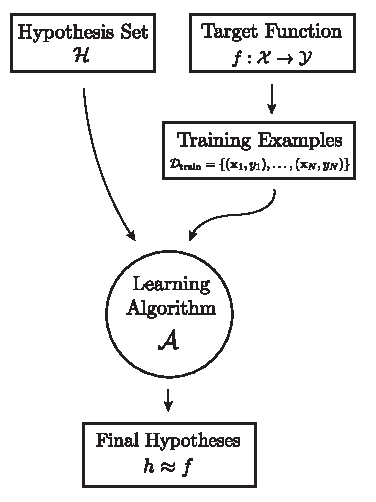
\includegraphics[width=0.99\textwidth]{figures/learning_problem/learning_problem.pdf}
  \caption[The Learning Problem]
    {Schematic overview of the learning problem and how to find the optimal hypothesis $h^*$ to approximate $f$ given the training data $\mathcal{D}_\mathrm{train}$.
    }
  \label{fig:ml:learning_problem}
\end{marginfigure}

Without any loss of generality, let the focus for now be on classification. The goal is to find the underlying \q{true} function $f: \mathcal{X} \mapsto \mathcal{Y}$ that predicts the correct label $y$ for each observation $\vec{x}$. This function is unknown and although it is impossible to find $f$, it is possible to learn an approximation of it, $h$, based on some training observations $\mathcal{D}_\mathrm{train} = \left \{(\vec{x}_1, y_1), \dots, (\vec{x}_N, y_N) \right\}$. The optimal hypothesis, $h^*$, is chosen among a set of $K$ candidate hypotheses $\mathcal{H} = \left\{h_1, h_2, \ldots, h_K  \right\}$, and hopefully $h^*$ will be a good approximation of $f$: $h^* \approx f$. A schematic overview of this process is shown in Figure~\ref{fig:ml:learning_problem}. 

How can one make sure that $h^*$ really is a good approximation of $f$? That is where statistical learning theory comes into play. From a statistical standpoint, we are interested in modelling the unknown joint probability $P(\vec{x}, y)$ over $\mathcal{X}$ and $\mathcal{Y}$. Assuming that $\mathcal{D}_\mathrm{train}$ is independent and identically distributed (\emph{iid})\sidenote[][3mm]{This is one of the two key assumptions of statistical learning theory, the other being that future events are coming from the same distrubution as the one that generated the past events. These assumptions are sometimes called the \emph{PAC} assumptions where PAC is an abbreviation for Probably, Approximately Correct, \autocite{AdvancedTopicsMachine}.} from $P(\vec{x}, y)$, we want to find the hypothesis whose predictions $h(\vec{x})=\hat{y}$ matches the conditional probability distribution $P(y|\vec{x})$ as well as possible. 

To quantify the statement \q{as well as possible} in the previous paragraph, we define the loss function $\ell$ which measures the loss for predicting $\hat{y}$ instead of $y$: $\ell(\hat{y}, y) = \ell(h(\vec{x}), y) \in \mathbb{R}^+$. Given $\ell$, we now introduce the method of (empirical) risk minimization \citep{vapnikPrinciplesRiskMinimization1991} and the expected loss\sidenote[][2mm]{Also called expected error or the out-of-sample error.} $L(h)$:
\begin{equation} 
  \label{eq:L}
  L(h) = \mathbb{E} \left[\ell(h(\vec{x}), y) \right] = \int \ell(h(\vec{x}), y)  \, dP(\vec{x}, y).
  \end{equation}
The optimal hypotheses $h^*$ is the hypothesis which minimizes the expected loss. However, the joint probability distribution $P(\vec{x}, y)$ is unknown and we are thus left with the empirical loss\sidenote{Also called the empirical error.} of $h$ on $\mathcal{D}_\mathrm{train}$:
\begin{equation}
  \label{eq:L_hat}
  \hat{L}(h, S) = \frac{1}{N} \sum_{i=1}^{N} \ell(h(\vec{x}_i), y_i), % \equiv \mathcal{L} 
\end{equation}
which is an approximation of $L(h)$ based on the training data available. 
% In the remainder of the text $\hat{L}(h, S)$ and $\mathcal{L}$ will be used interchangeably. 
Now the optimal hypothesis $h^*$ can defined:
\begin{equation}
  h^* = \argmin_{h\in\mathcal{H}} \hat{L}(h, S).
\end{equation}

\section{Generalization Bound}
\label{sec:generalization_bound}
In the previous section, the method of selecting the optimal hypothesis $h^*$ out of the total set of candidate hypotheses $\mathcal{H}$ was sketched. However, there is still no guarantee that $h^*$ will work well, that is to say that the \emph{generalization error} $G(h)$ might be big:
\begin{equation}
  G(h) = \hat{L}(h, S) - L(h).
\end{equation}
The generalization error is thus the difference between the expected error $L(h)$ and the empirical error $\hat{L}(h, S)$. It describes the loss in performance of our chosen model compared to the optimal, yet hidden, model. Since $P(\vec{x}, y)$ is unknown, $G(h)$ cannot be computed, however, it is possible to bound this error using statistical learning theory. To do so, the union bound and Hoeffding's (one-sided) inequalities are introduced. 
\begin{lemma}[The Union Bound]
  For any finite or countably infinite sequence of events $E_1, E_2, \dots$ (not necessarily independent): 
  \begin{equation}
    \mathbb{P} \left\{\bigcup_{1 \leq i} E_i \right\} \leq \sum_{1 \leq i} \mathbb{P} \left\{E_i \right \}. 
  \end{equation}
\end{lemma}
The union bound, in simple terms, states that the probability of any one of $n$ events happening is less than or equal to the sum of the individual probabilities of the events happening. As an example, let $E_1=\{2, 4, 6\}$ be the event that a die rolls an even number and $E_2=\{4, 5, 6\}$ be the event that a die rolls a number larger than or equal to $4$. Then $\mathbb{P} \left\{E_1 \cup E_2 \right\} = \mathbb{P} \left\{ 2, 4, 5, 6 \right\} \leq \mathbb{P} \left\{E_1 \right \} + \mathbb{P} \left\{E_2 \right \} $. 
\begin{lemma}[The one-sided Hoeffding's inequalities]
  Let $Z_1, \dots, Z_N$ be independent random variables each belonging to the $[0, 1]$ interval such that $\mathbb{P}\left\{Z_i \in [0, 1] \right\} = 1$ and $\mathbb{E}[Z_i] = \mu$ for all i, then for every $\epsilon > 0$:
  \begin{equation}
    \mathbb{P} \left\{  \frac{1}{N}\sum_{i=1}^N Z_i - \mu \geq \epsilon \right\} \leq e^{-2N\epsilon^2} 
    \label{eq:hoeffding_onesided_a}
  \end{equation}
  and
  \begin{equation}
    \mathbb{P} \left\{ \mu - \frac{1}{N}\sum_{i=1}^N Z_i  \geq \epsilon \right\} \leq e^{-2N\epsilon^2}.
    \label{eq:hoeffding_onesided_b}
  \end{equation}
\end{lemma}
When using the union bound on equation \eqref{eq:hoeffding_onesided_a} and \eqref{eq:hoeffding_onesided_b} we arrive at Hoeffding's (two) sided inequality:
\begin{lemma}[The two-sided Hoeffding's inequality]
  \label{lemma:hoeffding}
  Let $Z_1, \dots, Z_N$ be independent random variables each belonging to the $[0, 1]$ interval such that $\mathbb{P}\left\{Z_i \in [0, 1] \right\} = 1$ and $\mathbb{E}[Z_i] = \mu$ for all i, then for every $\epsilon > 0$:
  \begin{equation}
    \mathbb{P} \left\{ \left| \frac{1}{N}\sum_{i=1}^n Z_i - \mu \right| \geq \epsilon \right\} \equiv \mathbb{P} \left\{ \left| \hat{\mu} - \mu \right| \geq \epsilon \right\} \leq 2 e^{-2N\epsilon^2},
    \label{eq:hoeffding_inequality}
  \end{equation}
  where we have defined the empirical average $\hat{\mu}$ of $Z$ to be: $\hat{\mu}=\frac{1}{n}\sum_{i=1}^N Z_i$.
\end{lemma}
Assuming that the loss $\ell(\hat{y}, y)$ is bounded in the $[0, 1]$ interval\sidenote{Which it is for classification, however, it can be extended in a similar fashion for regression.}, the generalization error $G(h)$ is bound by letting $Z_i = \ell(\hat{y}_i, y_i) = \ell(h(\vec{x}_i), y_i)$ be the loss of $h$ in sample $(\vec{x}_i, y_i)$. By comparing Lemma \ref{lemma:hoeffding} and equation \eqref{eq:L_hat}, we see that $\hat{\mu} = \hat{L}(h, S)$, and similar for equation \eqref{eq:L}: $\mu = L(h)$. We then see that the generalization error is bounded:
\begin{equation}
  \label{eq:hoeffding_inequality_generalization_error}
  \mathbb{P} \left\{ \left| G(h) \right| \geq \epsilon \right\} = \mathbb{P} \left\{ \left| \hat{L}(h, S) - L(h) \right| \geq \epsilon \right\} \leq 2 e^{-2N\epsilon^2}.
\end{equation}
This equation provides a bound on the difference between the empirical loss and the expected loss. 
% Say the probability of the generalization error being larger than $\epsilon = 0.1$ is needed for $N=100$ samples, we find that the this probability is $P=27\%$. 
The generalization bound  can be rewritten in terms of $\delta$:
\begin{equation}
  \delta \equiv 2 e^{-2N\epsilon^2} \in (0, 1) \quad \Rightarrow \quad \epsilon = \sqrt{\frac{\ln \frac{2}{\delta}}{2N}}.
\end{equation}
\begin{theorem}[Hoeffding's inequality for a single hypothesis]
  \label{theorem:hoeffding_single}
  Assume that $\ell$ is bounded in the $[0, 1]$ interval, then for a single hypothesis $h$ and any $\delta\in(0,1)$ we have:  
  \begin{equation}
    \label{eq:hoeffding_inequality_generalization_error_delta}
    \mathbb{P} \left\{ \left| \hat{L}(h, S) - L(h) \right| \geq \sqrt{\frac{\ln \frac{2}{\delta}}{2N}}  \right\} \leq \delta.
  \end{equation}
\end{theorem}
Equation \eqref{eq:hoeffding_inequality_generalization_error_delta} can be read as the probability of the generalization error being larger than $\sqrt{\frac{\ln \frac{2}{\delta}}{2N}}$ is $\delta$ or less, or, similarly, that with probability greater than $1-\delta$:
\begin{equation}
  \label{eq:hoeffding_inequality_single_PAC}
  \left| \hat{L}(h, S) - L(h) \right| \leq \sqrt{\frac{\ln \frac{2}{\delta}}{2N}}.
\end{equation}
This is a powerful result relating the performance of a (fixed) hypothesis $h$ with the number of samples, $N$. We see that a higher $N$ yields a tighter bound on the generalization error.
% inversely\sidenote{Not to be understood as $1/x$ in this context.} related to on the certainty\sidenote{Technically the certainty of the model is $1-\delta$.} $\delta$ of this bound.

There is a big assumption of this derivation: that the hypothesis $h$ cannot depend on the sample $S$ and thus has to be chosen before seeing the data. We say that $h$ has to be \emph{fixed}. Of course the term machine learning indicates that some kind of learning is taking place: exactly as seen previously where we wanted to find the optimal hypotheses $h^*$ out of all the possible ones $\mathcal{H}$. For now assume that $\mathcal{H}$ is finite and consists of $K$ hypotheses: $|\mathcal{H}| = K$. We thus have $[h_1, h_2, \dots, h_K]$ hypotheses which we test simultaneously and where Hoeffding's inequality is true for each of them leading to the following theorem:
\begin{theorem}[Hoeffding's inequality for a finite set of hypotheses candidates]
  \label{theorem:hoeffding_finite}
  Assume that $\ell$ is bounded in the $[0, 1]$ interval and that $|\mathcal{H}| = K$. Then for any $\delta\in(0,1)$ we have:  
  \begin{equation}
    \label{eq:hoeffding_inequality_theorem_multiple}
    \mathbb{P} \left\{ \exists h \in \mathcal{H}: \left| \hat{L}(h, S) - L(h) \right| \geq \sqrt{\frac{\ln \frac{2K}{\delta}}{2N}}  \right\} \leq \delta.
  \end{equation}
\end{theorem}

\marginnote[-1cm]{Here \q{$\exists x : y$} means that there exists at least one $x$ such that $y$ is true.}

\begin{proof}
  The proof begins by denoting $h_i$ as the event where: 
  \begin{equation*}
    \left| \hat{L}(h_i, S) - L(h_i) \right| \geq \sqrt{\frac{\ln \frac{2}{\delta'}}{2N}},
  \end{equation*}
   and then taking the union bound (the first inequality below) followed by applying Hoeffding's inequality to each part in the sum (the second inequality): 
\begin{equation*}
  % \label{eq:hoeffding_inequality_generalization_error_delta}
  \begin{split}
    \mathbb{P} \Biggl\{ \exists h \in \mathcal{H}: \left| \hat{L}(h, S) - L(h) \right| &\geq \sqrt{\frac{\ln \frac{2}{\delta'}}{2N}}  \Biggr\} \\
    &= \mathbb{P} \left\{ \bigcup_{h \in \mathcal{H}} \left| \hat{L}(h, S) - L(h) \right| \geq \sqrt{\frac{\ln \frac{2}{\delta'}}{2N}}  \right\}  \\
    &\leq \sum_{h \in \mathcal{H}} \mathbb{P} \left\{\left| \hat{L}(h, S) - L(h) \right| \geq \sqrt{\frac{\ln \frac{2}{\delta'}}{2N}} \right\}  \\
    &\leq \sum_{h \in \mathcal{H}} \delta' \\
    &= K \delta'.
  \end{split}
\end{equation*}
By making the substitution $\delta = K \delta'$ we arrive at equation \eqref{eq:hoeffding_inequality_theorem_multiple}. 
\end{proof}

As we did in equation \eqref{eq:hoeffding_inequality_single_PAC}, equation \eqref{eq:hoeffding_inequality_theorem_multiple} can also be read as with probability greater than $1-\delta$, then for all $h\in\mathcal{H}$:
\begin{equation}
  \label{eq:hoeffding_inequality_multi_PAC}
  \left| \hat{L}(h, S) - L(h) \right| \leq \sqrt{\frac{\ln \frac{2K}{\delta}}{2N}}.
\end{equation}
This bound is looser than the one for only a single hypothesis by a factor $\ln K$, however, this holds for the optimal hypothesis $h^*$. 

\subsection{Generalization Bound for Infinite Hypotheses}
\label{subsec:generalization_bound_infinite}
Section \ref{sec:generalization_bound} dealt with the case of a single hypotheses $h$ and a finite set of candidate hypotheses $h\in\mathcal{H}, |\mathcal{H}| = K$. When $K$ goes towards infinity the generalization bound goes to infinity and the bound becomes useless. However, even some simple models such as a linear classifier\sidenote{Also known as the perceptron. Often includes the constant offset $b$ which is omitted here for brevity. The functional form of this function is $f(x)=\mathrm{sign}(\vec{w}^T\vec{x})$.} that predicts $\hat{y}=1$ when the dot product $\vec{w}^T\vec{x}$ is positive and $\hat{y}=-1$ when it is negative, has $|\mathcal{H}| = \infty$. Since an infinite number of hypotheses $h(\vec{w})$ exists, assuming we allow $\vec{w}$ to take any real values as is almost always the case, $\mathcal{H}$ is infinite. 

To solve this obvious problem with the Hoeffding inequality, we introduce the Vapnik-Chervonenkis (VC) generalization bound\sidenote{For proof, see: \citet{abu-mostafaLearningData2012}.}. The VC-bound is based on the so-called VC-dimension of the hypothesis space $\mathcal{H}$: $d_\mathrm{VC}(\mathcal{H}) \equiv d_\mathrm{VC}$. The VC-dimension is a measure of the complexity of the hypothesis space; the degrees of freedom of the model so to say. For example, the VC-dimension of the $M$-dimensional linear classifier defined above\sidenote{In the general case when the offset $b$ is included it is $d_\mathrm{VC}=M+1$.} is $d_\mathrm{VC}=M$ for $\{\vec{x}, \vec{w}\} \in \mathbb{R}^M$. 
\begin{theorem}[VC Generalization Bound]
  \label{theorem:VC_generalization_bound}
  Let $\mathcal{H}$ be a hypotheses class with VC-dimension: $d_\mathrm{VC}(\mathcal{H}) = d_\mathrm{VC}$. Then with probability at least $1-\delta$: 
  \begin{equation}
    \label{eq:VC_bound}
    L(h) \leq \hat{L}(h, S) + \sqrt{ \frac{8}{N} \ln \left( \frac{4}{\delta} \left( \left(2N \right)^{d_\mathrm{VC}} + 1 \right)  \right)} .
  \end{equation}
\end{theorem}
Equation \eqref{eq:VC_bound} states that the out of sample error $L(h)$ is bounded from above by the empirical error $\hat{L}(h, S)$ and second term which is related to the complexity of the hypothesis space $\mathcal{H}$, the number of samples $N$ and the certainty $\delta$. This is called the model complexity penalty $\Omega(N, \mathcal{H}, \delta)$:
\begin{equation}
  \Omega(N, \mathcal{H}, \delta) = \sqrt{ \frac{8}{N} \ln \left( \frac{4}{\delta} \left( \left(2N \right)^{d_\mathrm{VC}(\mathcal{H})} + 1 \right)  \right)}.
\end{equation}
As the hypothesis space complexity, $d_\mathrm{VC}$, grows, the model complexity penalty increases but it is more likely that $\mathcal{H}$ contains a strong hypothesis. This relationship is called the approximation-estimation or the  \emph{bias-variance} tradeoff. When the model is too simple to properly fit the complexity in the data, it is called \emph{underfitting}\sidenote{Here the error from $\hat{L}(h, S)$ dominates.}. When the model is so complex that it starts fitting the inherent noise in the data, it is called \emph{overfitting}\sidenote{Here the error from $\Omega(N, \mathcal{H}, \delta)$ dominates.}. The loss as a function of model complexity gives the characteristic curve illustrated in Figure~\ref{fig:ml:empirical_risk}. As the model complexity increases, the training loss decreases. Initially, also the validation loss decreases, but at some point the behavior of the model on the validation set worsens and the loss increases; overfitting happens. 

\begin{marginfigure}
  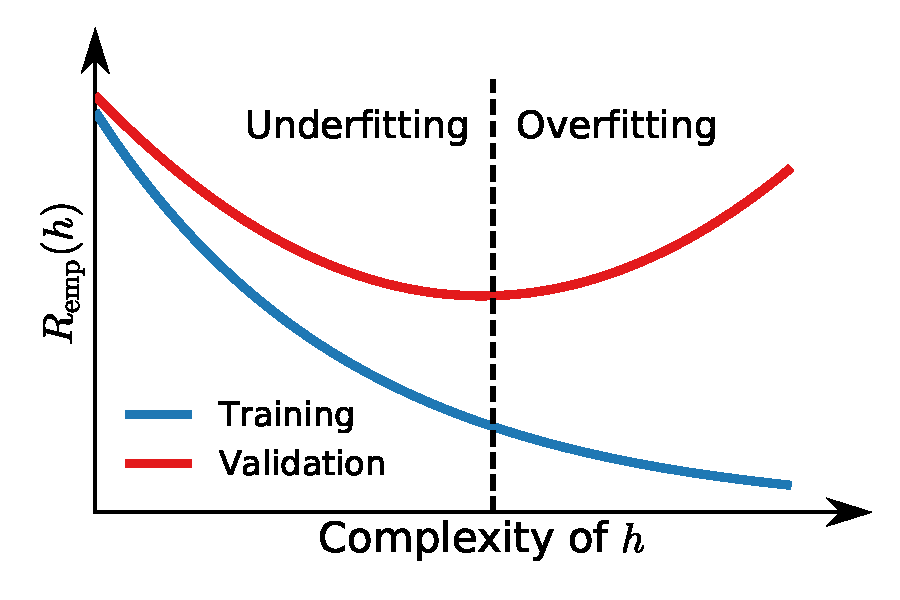
\includegraphics[width=0.98\textwidth]{figures/overfitting/overfitting_1.pdf}
  \caption[Approximation-Estimation Tradeoff]
    {Illustration of the empirical loss as a function of model complexity. The \textcolor{blue}{training error} is shown in blue and \textcolor{red}{validation error} in red.
    }
  \label{fig:ml:empirical_risk}
\end{marginfigure}


\section{Avoiding overfitting}
\label{sec:ml:overfitting}
Avoiding overfitting is one of the most important issues in machine learning. By now, most modern machine learning algorithms have the inherent model complexity needed for overfitting and it thus has to be managed. Due to the importance of the issue, a number of different methods exists which reduce overfitting. Most of them are complementary of each other and can be taken advantage of in a combination. Model regularization will be introduced in \autoref{subsec:regularization}, cross validation in \autoref{subsec:cross_validation}, and early stopping in \autoref{subsec:early_stopping}. 

\subsection{Model Regularization}
\label{subsec:regularization}
One of the earliest methods developed for preventing overfitting was model regularization. A. N. Tikhonov \citep{tikhonovStabilityInverseProblems1943} was one of the first to describe this method in \num{1943}. In particular, regularization was used to solve \emph{ill posed}\sidenote{The definition of \q{ill posed} is given in further down.} linear regression problems. Regular linear regression problems refer to minimizing the residual sum of squares written in matrix form as:
\begin{equation}
  \begin{split}
    \hat{\bm{\beta}}_{\mathrm{LS}} = \argmin_{\bm{\beta}} \norm{\vec{y} - \vec{X} \bm{\beta} }_2^2 = \argmin_{\bm{\beta}} \norm{ \vec{y} - \vec{f}(\vec{X}) }_2^2 \\
    \vec{f}(\vec{X}) = \vec{X} \bm{\beta}.
  \end{split}
\end{equation}

Here $\vec{y}$ is the vector of values we are trying to predict\sidenote{E.g. the prices of a collection of houses.}, $\vec{X}\in\mathbb{R}^{N\times M}$ is the matrix of input variables, $\hat{\bm{\beta}}_{\mathrm{LS}}$ is the vector of unknown coefficients\sidenote{Here excluding the constant offset $\beta_0$ which can be included trivially.} of the linear least squares (LS) model $\vec{f}$, and $\norm{ \bm{\cdot} }_2$ is the normal Euclidean norm. In general, the $p$-norm is defined as:
\begin{equation}
  \norm{\vec{x}}_p = \left( \sum_{i=1}^N \abs{x_i}^p \right)^{1/p}.
\end{equation}

Differentiating the objective $\norm{\vec{y} - \vec{X} \bm{\beta} }_2^2$ with respect to (w.r.t.) $\bm{\beta}$, and setting the derivative equal to $0$ to find the minimum\sidenote{When checking the double derivative wrt. $\bm{\beta}$ it is seen that this really is a minimum and not a maximum (or saddle point).}, yields the solution for $\bm{\beta}$:
\begin{equation}
  \begin{split}
    \frac{\partial}{\partial \bm{\beta}} \norm{\vec{y} - \vec{X} \bm{\beta} }_2^2 = -2 \vec{X}^T \left( \vec{y} - \vec{X} \bm{\beta} \right) = 0  \Rightarrow \\
    \vec{X}^T \vec{y} - \vec{X}^T \vec{X} \bm{\beta} \Rightarrow \\
    \hat{\bm{\beta}}_{\mathrm{LS}} =  \left( \vec{X}^T \vec{X} \right)^{-1} \vec{X}^T \vec{y}.
  \end{split}
\end{equation}

However, this solution for $\hat{\bm{\beta}}_{\mathrm{LS}}$ is only valid when $\vec{X}^T \vec{X}$ is invertible, i.e. $\vec{X}$ has to be full rank \citep{hastieElementsStatisticalLearning2009}. If this is not the case, the problem is said to be ill posed. Tikhonov solved this problem by adding an extra term to the minimization problem, which we will call $\Omega$ for simplicity. For a specific choice of $\Omega = \lambda \norm{ \bm{\beta} }^2_2$, one gets:
\begin{equation}
  \label{eq:l2_norm}
  \hat{\bm{\beta}}_{\mathrm{L_2}} = \argmin_{\bm{\beta}} \left \{\norm{ \vec{y} - \vec{f}(\vec{X}) }_2^2 + \lambda \norm{ \bm{\beta} }^2_2 \right \},
\end{equation}
where $\lambda \geq 0$ is the regularization strength. This is the so-called $L_2$-regularization, also known as ridge regression for linear problems. For ridge regression the corresponding solution for $\bm{\beta}$ is\sidenote{Here $\hat{\bm{\beta}}_{\mathrm{L_2}}$ is the solution for any general function $\vec{f}$ and $\hat{\bm{\beta}}_{\mathrm{ridge}}$ is the specific solution for a linear function $\vec{f}$, where linear is w.r.t. the model parameters $\bm{\beta}$.}:
\begin{equation}
  \label{eq:l2_norm_linear}
  \hat{\bm{\beta}}_{\mathrm{ridge}} =  \left( \vec{X}^T \vec{X} + \lambda \vec{I} \right)^{-1} \vec{X}^T \vec{y},
\end{equation}
where $\vec{I}$ is the identity matrix\sidenote{The $\lambda \vec{I}$ in equation \eqref{eq:l2_norm_linear} also acts as a conditioner on the problem in the sense that it reduces the condition number of the matrix to be inverted turning the ill-posed problem to a well-behaved one.}. The extra term, $\Omega =  \lambda \norm{ \bm{\beta} }^2_2$, in equation \eqref{eq:l2_norm} acts as a shrinkage factor on the coefficients of $\bm{\beta}$. Looking at this equation, we see that this is the Lagrangian form of the equivalent problem: 
\begin{equation}
  % \label{eq:ml:constrained_minimization_L2}
  \begin{split}
    \hat{\bm{\beta}}_{\mathrm{L_2}} = \argmin_{\bm{\beta}} \norm{ \vec{y} - \vec{f}(\vec{X}) }_2^2 \\
    \mathrm{subject~to:} \quad \sum_{i=1}^N \beta_i^2 = \norm{\bm{\beta}}^2_2 \leq t,
  \end{split}
  \label{eq:l2_norm_non_lagrangian}
\end{equation}

\begin{marginfigure}[5mm]
  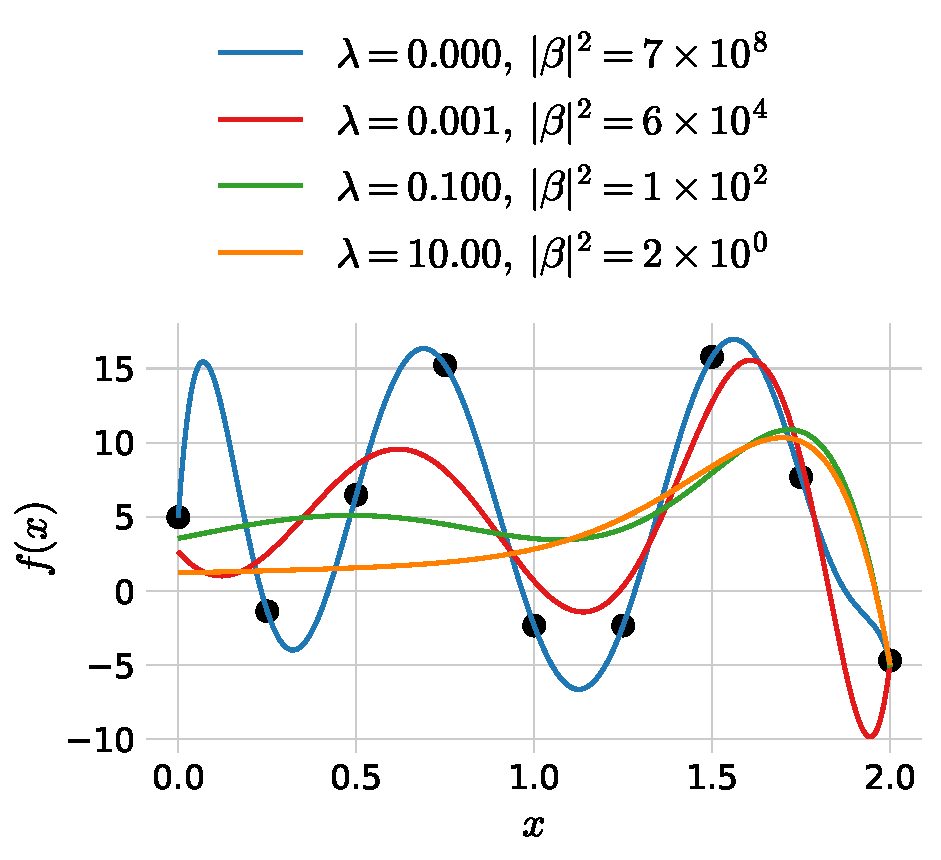
\includegraphics[width=0.99\textwidth, trim=5 5 5 5, clip]{figures/ridge_regression/ridge.pdf}
  \caption[Regularization Strength]
    {Effect of tuning the regularization strength $\lambda$ in ridge regression.
    }
  \label{fig:ml:regularization_ridge}
\end{marginfigure}

\noindent for some $t \geq 0$ with a one-to-one mapping between $\lambda$ and $t$. We thus see that $L_2$ regularizes the coefficients of $\bm{\beta}$ to have some maximal norm. The effect of the regularization is controlled by $\lambda$, where $\hat{\bm{\beta}}_{\mathrm{L_2}} \rightarrow \hat{\bm{\beta}}_{\mathrm{LS}}$ for $\lambda \rightarrow 0$ and $\hat{\bm{\beta}}_{\mathrm{L_2}} \rightarrow \vec{0}$ for $\lambda \rightarrow \infty$. An example of this is shown in Figure~\ref{fig:ml:regularization_ridge}. Here $N=9$ datapoints were randomly generated such that the $x$-values are evenly spaced from \num{0} to \num{2} and $y \sim \mathcal{N}(\mu=0, \sigma=10)$. They were fit with a \num{9}-order polynomial by minimizing equation \eqref{eq:l2_norm} for different values of $\lambda$. We see the regularizing effect of $\lambda$, going from $\lambda=0$ in blue which fits all points\sidenote{Since the order of the polynomial is the same as the number of datapoints.} with a high degree of variance and a wildly oscillatory pattern, to $\lambda=10$ in orange which is mostly flat in most of the interval. Also note in the legend how the norm of the fit parameters also decrease with $\lambda$, as expected. This is a great example of the \emph{bias-variance} tradeoff mentioned in \autoref{subsec:generalization_bound_infinite}, where bias refers the error the model makes when it is not advanced enough to fit the overall trend in the data (underfitting) and variance refers to the error that the model makes when it starts to fit spurious noisy fluctuations in the training set which are not present in the validation set (overfitting). 
% In this example $\lambda=0$ is clearly overfitting the data whereas $\lambda=10$ is an example of underfitting. 

\begin{marginfigure}[0.9cm]
  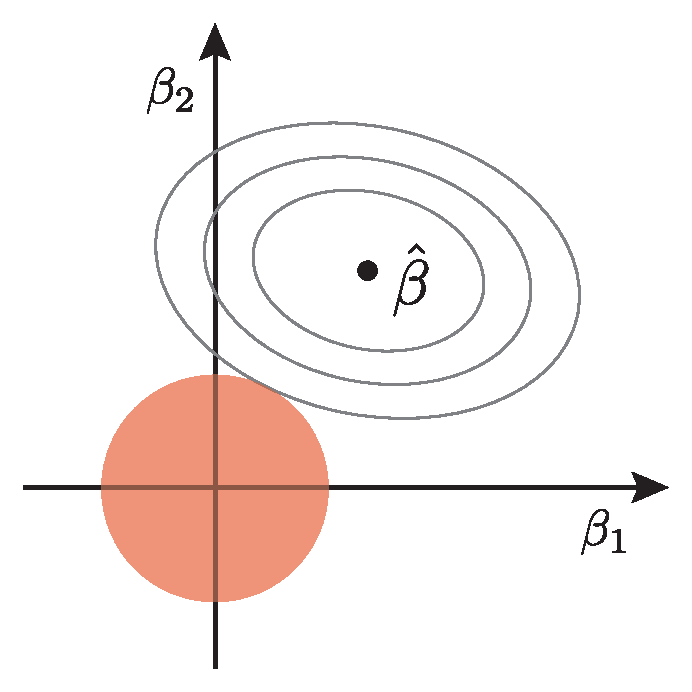
\includegraphics[width=1\textwidth]{figures/ridge_lasso_sparse/ridge.pdf}
  \caption[Regularization Effect of $L_2$ ]
    {Sketch of the minimization problem defined in equation \eqref{eq:l2_norm_non_lagrangian}, i.e. for a $L_2$-penalty. The \textcolor{red}{constrain region} shown in red is defined as $\beta_1^2 + \beta_2^2 \leq t$ for $L_2$ in $2D$-space and the contours of the unconstrained solution is shown with grey lines. Adapted from \autocite{hastieElementsStatisticalLearning2009}.
    }
  \label{fig:ml:regularization_effect_ridge}
\end{marginfigure}

Other values of the regularization function $\Omega$ exists, for example the $L_1$-penalty:
\begin{equation}
  \Omega = \lambda \norm{\bm{\beta}}_1, 
\end{equation}
where the 1-norm, also known as Manhattan norm, is used. In the case of linear problems, the $L_1$-penalty leads to Lasso regression introduced by \citet{tibshiraniRegressionShrinkageSelection1996} in \num{1996}. As with the $L_2$-penalty, the $L_1$-penalty also regularizes the coefficients of $\bm{\beta}$, however, this penalty leads to sparse\sidenote[][1cm]{Meaning that a number (depending on $\lambda$) of the $\beta_i$ coefficients are 0.} solutions. An illustration of this is shown in Figure~\ref{fig:ml:regularization_effect_ridge} and Figure~\ref{fig:ml:regularization_effect_lasso} where the constraint regions of $\bm{\beta}$ are shown in red, and the grey ellipses are the contours of the non-constrained problem. Notice how the intersection of the contour lines and the constrain region leads to $\beta_1 \neq 0, \beta_2 \neq 0$ for the $L_2$-penalty whereas it leads to the sparse solution $\beta_1=0, \beta_2 \neq 0$ for the $L_1$-penalty. This is a general pattern seen for $L_p$-penalties for $p \leq 1$ \autocite{hastieElementsStatisticalLearning2009}.

\begin{marginfigure}[0.5cm]
  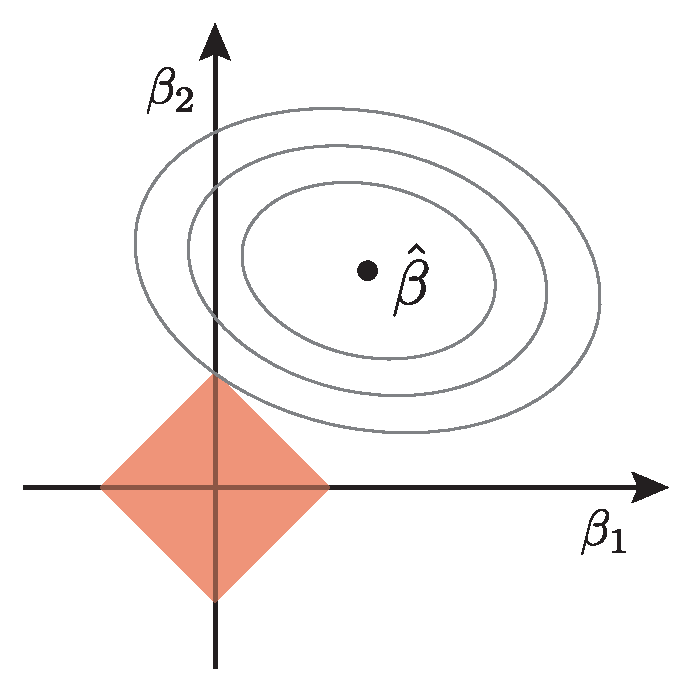
\includegraphics[width=1\textwidth]{figures/ridge_lasso_sparse/lasso.pdf}
  \caption[Regularization Effect of $L_1$]
    {Sketch of the similar minimization problem defined in Figure~\ref{fig:ml:regularization_effect_ridge} for the $L_1$-penalty. The \textcolor{red}{constrain region} shown in red is defined as $\abs{\beta_1} + \abs{\beta_2} \leq t$ for $L_1$ in $2D$-space and the contours of the unconstrained solution is shown with grey lines. Adapted from \autocite{hastieElementsStatisticalLearning2009}.
    }
  \label{fig:ml:regularization_effect_lasso}
\end{marginfigure} 

Overall, model regularization is heavily used in modern machine learning algorithms. In general, the function or the so-called \emph{objective function} $\mathcal{L}$ they are trying to minimize is:
\begin{equation}
  \mathcal{L}(h) = \hat{L}(\ell, h, S) + \Omega(h, \lambda)
\end{equation}
where $\hat{L}$ is the empirical loss and $\Omega$ is the regularization penalty. 

Choosing the right value for the regularization strength is a fundamental problem in model regularization. How to choose a suitable value for $\lambda$ via cross validation is discussed in \autoref{subsec:cross_validation} and the choice of the training loss function $\ell$ in \autoref{sec:ml:loss_function}. 

\subsection{Cross Validation}
\label{subsec:cross_validation}
In general we want to  be able to estimate the performance\sidenote{\q{Performance} is used here as the word for the general metric to be optimized for, whether or not this metric should be maximized or minimized.} of the developed model. Since evaluating the model on the data it was already trained on would give a biased estimate of the performance, we need an unbiased method of doing so. The easiest way would be to set a fraction of the data aside, e.g. \SI{20}{\percent}, train on the remaining part and then evaluate the performance on the data set aside. Splitting the data up like this would provide us with a training (data)set and a test set in a $(80/20)\%$ ratio. This would then yield an unbiased performance estimate when evaluation the performance on the test set. 
However, if one then needed to compare two different models -- with e.g. different values of regularization strength $\lambda$ -- and choose the best one, as is often the case, this method would not work since we would choose the model with the best performance on the test set. This can be seen as training on the test set and thus it has \q{tainted} the purity of the test set. To avoid this, an additional split is made such that we get a training set, a validation set, and a test set, where you often see a $(80/10/10)\%$ ratio. The two models can then be compared on the validation set and the performance of the chosen model can be estimated from the test set. 



This way of splitting up the data has some clear benefits and is thus also often used. There is a drawback, however, and that is that we are not fully utilizing a lot of the data in this way. Basically, \SI{20}{\percent} of the data are only used to provide a single number of performance and does not necessarily allow an uncertainty or confidence interval of this measurement to be calculated. Thus, other methods of estimating model performance are developed. 

\begin{marginfigure}[1cm]
  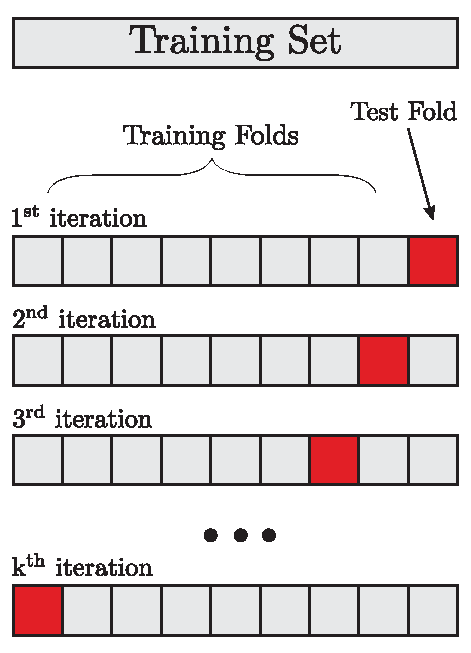
\includegraphics[width=\textwidth, trim=5 5 5 5, clip]{figures/cross_validation/kfold.pdf}
  \caption[$k$-Fold Cross Validation]
    {$k$-fold cross validation. 
    }
  \label{fig:ml:cross_val_kfold}
\end{marginfigure} 

One of the most used and well-known ones is the $k$-fold cross validation (CV). In $k$-fold cross validation the entire dataset is split up into $k$ chunks which are randomly drawn subsamples (without replacement). In the first iteration, the model is trained on the first $k-1$ subsamples and evaluated on the last $k$ subsample. In the second iteration the evaluation subsample is a new one. This process is continued $k$ times until all samples in the dataset have been trained and evaluated on \citep{hastieElementsStatisticalLearning2009}. For an illustration of this, see Figure~\ref{fig:ml:cross_val_kfold}. 

The process yields $k$ estimates of the performance of the model which can then be averaged to form a single performance number and the variability of the performance can even be gauged\sidenote{Special care has to be taken here since the $k$ different performance values are not independent.}. The disadvantage of $k$-fold CV is that the performance estimate is now slightly biased, however, this effect is generally very small. The biggest disadvantage is the computational burden related to doing $k$-fold CV where $k\gg 1$. A compromise often used in applied machine learning is $k=5$ which is also what is used in this project.  

Special care has to be taken when dealing with time series data. Here the problem of \emph{data leakage} is often introduced inadvertently. Data leakage is when the model is exposed to information from the test set that it was not supposed to be exposed to. In the case of time series data, if the data is split by the usual $k$-fold CV, then each subsample contains events from all times and the model does not learn how to predict future events. To circumvent this problem, a special type of $k$-fold CV for time series data has to be used. Here all samples up to a specific time, eg. all houses sold before 2018, is used for training and then the model is evaluated on the performance of samples after the event, e.g. houses sold in \num{2018}. For an illustration of this, see Figure~\ref{fig:ml:cross_val_kfold_time}.

\begin{marginfigure}[-6cm]
  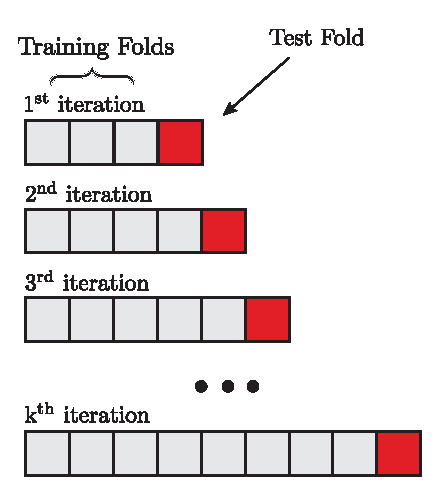
\includegraphics[width=\textwidth, trim=5 5 5 5, clip]{figures/cross_validation/kfold_time.pdf}
  \caption[$k$-Fold Cross Validation for Time Series Data]
    {$k$-fold cross validation for time series data. 
    }
  \label{fig:ml:cross_val_kfold_time}
\end{marginfigure} 

\subsection{Early Stopping}
\label{subsec:early_stopping}
Most modern machine learning models are trained iteratively. This is the case for both (boosted) decision trees and neural networks, both of which are used in this project. In this context, iteratively means that the model starts off with an initial guess of the parameters of the model and \q{learns} a new and better set of values by looking at the data. The question then becomes: for how long should the model be allowed to continue training?

This is a another example of the bias-variance tradeoff. The model should be trained long enough to be able to capture the complexity inherent in the data but also should not train for so long that it starts to overfit the data. Even though Figure~\ref{fig:ml:empirical_risk} was just an illustration of the bias variance tradeoff, it is also something that is seen in real data and can be taken advantage of through \emph{early stopping}. Early stopping is the process of monitoring the loss for the training set $\mathcal{D}_\mathrm{train}$ and validation set $\mathcal{D}_\mathrm{val}$. The model is only fitted on $\mathcal{D}_\mathrm{train}$ but the performance on $\mathcal{D}_\mathrm{val}$ is measured simultaneously. Whenever the validation loss starts to increase, the training of the model should be terminated. 

To avoid stopping due to a single noise-induced outlier which terminated the process, one often uses \emph{patience} in the early stopping process: if the loss has not decreased since the last minimum after \emph{patience} number of iterations the process is terminated. Early stopping is thus an easy way of avoiding overfitting for iteratively trained models that only requires a validation set.  

\section{Loss functions}
\label{sec:ml:loss_function}
How we evaluate the performance of a model is of course very important since it defines the metric for the problem; what is good and what is bad? Obviously, this depends on whether or not a classification problem or a regression problem is dealt with. Let us for now focus on the latter. Say that a house is estimated to cost \num{2} million DKK (\si{\Mkr}) but was sold for \SI{4}{\Mkr} Compare this to a house that was estimated to cost \SI{8}{\Mkr} but was sold for \SI{6}{\Mkr} In both cases the price was off by \SI{2}{\Mkr}, but does this mean that both predictions are equally good or bad? The first case was off by a factor of \num{2}, whereas the prediction in the second case was only off by $33\%$ (compared to the true value). The first case underestimated the price whereas the second overestimated; should this have any importance?

As it should be clear by now, the choice of loss function $\ell$ is of utmost importance. It is also not a problem that can be solved by computers, it is problem-specific, and has to be defined manually. The choice of loss function is what is called a \emph{hyperparameter}, the optimization of which is further discussed in \autoref{sec:ml:hyperparameter_optimization}. The most common choice of loss function is by far the squared error (SE): 
\begin{equation}
  \ell_\mathrm{SE}(y, \hat{y}) = \left( y-\hat{y} \right)^2,
\end{equation}
where $y$ is the true value and $\hat{y}$ is the predicted one. Squared error has the advantage that it is differentiable everywhere, an effect that is both needed for many statistical derivations but also a requirement for some machine learning models. The disadvantage is that it gives too much weight to outliers since every deviation away from the truth is squared. In contrast to this, there is the absolute error (AE) defined as:
\begin{equation}
  \ell_\mathrm{AE}(y, \hat{y})  = \abs{y-\hat{y} }.
\end{equation}

For the absolute error, outliers have a lot smaller weight since it deals with the absolute value of the deviation and not the squared deviation. However, this comes at a price; the absolute error is not differentiable at every point. At $y-\hat{y} = 0$, the derivative of the absolute value function is un-defined. Many functions have been invented trying to deal with these problems. For a more general discussion of loss functions, see e.g. Barron \citep{barronGeneralAdaptiveRobust2017}. Six different loss functions (for regression problems) have been investigated in this project. In addition to the squared error and the absolute error also the LogCosh, Cauchy  \citep{barronGeneralAdaptiveRobust2017}, Welsch  \citep{barronGeneralAdaptiveRobust2017} and Fair  \citep{AllstateClaimsSeverity} loss functions are used:
\begin{equation}
  \begin{split}
    \label{eq:ml:loss_functions}
    \ell_\mathrm{LogCosh}(y, \hat{y})  &= \log\left( \cosh\left( y-\hat{y} \right) \right) \\
    \ell_\mathrm{Cauchy}(y, \hat{y})  &= \log\left( \frac{1}{2} \left(\frac{y-\hat{y}}{c}\right)^2 + 1   \right) \\
    \ell_\mathrm{Welsch}(y, \hat{y})  &=  1 - \exp\left( - \frac{1}{2} \left(\frac{y-\hat{y}}{c}\right)^2  \right)\\
    \ell_\mathrm{Fair}(y, \hat{y})  &= c^2  \left( \frac{\abs{y-\hat{y}} }{c}  - \log \left(\frac{\abs{y-\hat{y}}}{c} +1 \right )   \right). 
  \end{split}
\end{equation}
The above loss functions share some similarities with the absolute error, and, in addition to this, they are all (twice) differentiable functions. They are shown in Figure~\ref{fig:ml:objective_funcs}. They are shown for only positive values of $y-\hat{y}$ since they are symmetric in $y-\hat{y}$. Notice how the squared error quickly grows very large compared to the others. The absolute error has a kink at $y-\hat{y}=0$ as the only one of the functions. Welsch is bounded in the interval $[0, 1)$. The derivative of both LogCosh and Fair goes toward one when $y-\hat{y}$ goes towards infinity, whereas it goes to zero for the Cauchy loss. A priori, it is almost impossible to know which one of these loss functions performs best for a specific data set, so they have to be treated as hyperparameters. 

% \begin{marginfigure}[-5cm]
%   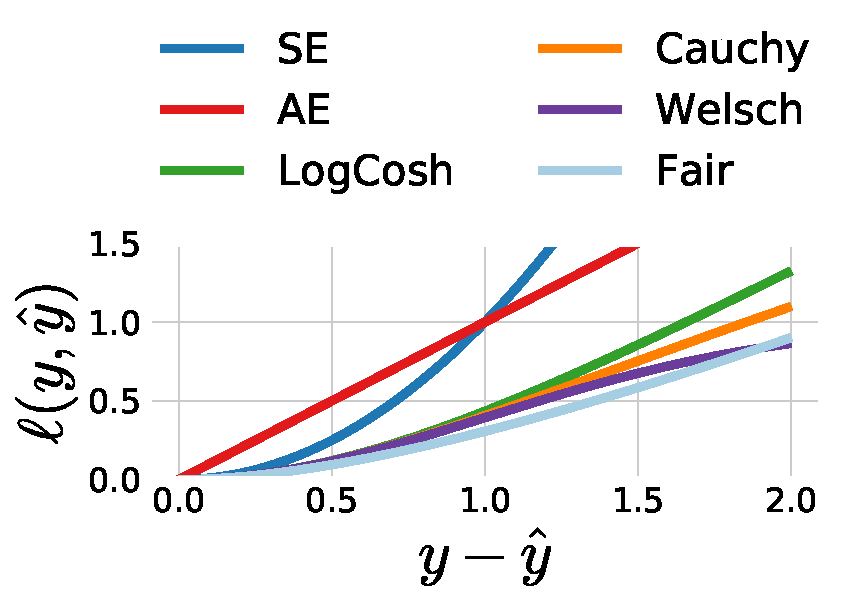
\includegraphics[width=0.98\textwidth]{figures/objective_functions/objective_functions_zoom.pdf}
%   \caption[Objective Functions Zoom In]
%     {Zoom in of \figref{fig:ml:objective_funcs}. 
%     }
%   \label{fig:ml:objective_funcs_zoom}
% \end{marginfigure}

\begin{figure}
  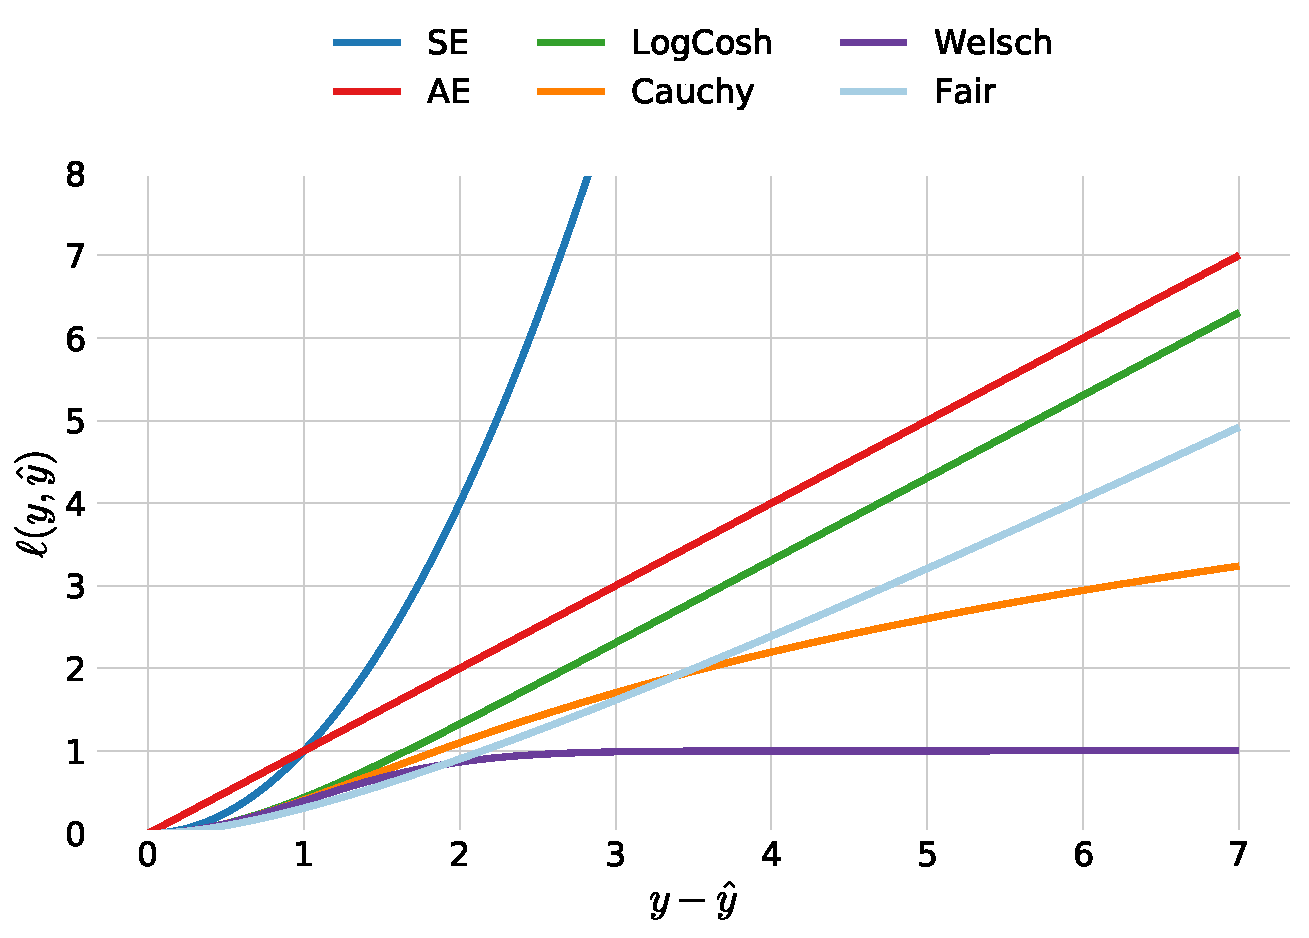
\includegraphics[width=0.9\textwidth]{figures/objective_functions/objective_functions.pdf}
  \caption[Objective Functions]
    {Comparison of the the six loss functions SE, AE, LogCosh, Cauchy, Welsch, and Fair as a function of $y-\hat{y}$, see equation \eqref{eq:ml:loss_functions}. In the plot \textcolor{blue}{SE} is shown in blue, \textcolor{red}{AE} in red, \textcolor{green}{LogCosh} in green, \textcolor{orange}{Cauchy} in orange, \textcolor{purple}{Welsch} in purple, and \textcolor{light-blue}{Fair} in light blue. For the Cauchy, Welsch, and Fair functions $c$ is set to 1. 
    % For a zoom in of the inner region where $y-\hat{y}<2$ see \figref{fig:ml:objective_funcs_zoom}. 
    All six graphs are symmetric in $y-\hat{y}$ which is why they are only shown for positive values of $y-\hat{y}$.
    }
  \label{fig:ml:objective_funcs}
\end{figure}


\subsection{Evaluation Function}
Since some machine learning models require an analytic expression for the derivative and second derivative, it not always possible to use a custom objective function if it is non-differentiable. The Area Under Curve (AUC) of the Receiver Operating Characteristic (ROC) is such a measure. Another example would be the width of the distribution of all $y_i-\hat{y}_i$. In this thesis the overall performance metric will be called the \emph{evaluation function}, $f_\mathrm{eval}$, compared to the differentiable proxy for this function, the objective function $\mathcal{L}$. To sum up: the loss function $\ell(y, \hat{y})$ measures the loss for an individual prediction and the objective function is the aggregated version of the individual losses. The objective function is assumed to be a good proxy for the evaluation function $f_\mathrm{eval}$ which is the overall metric.  
For the loss functions defined in \autoref{sec:ml:loss_function} the objective function is based on the mean of the individual losses:
\begin{equation}
  \mathcal{L} = \frac{1}{N} \sum_{i=1}^N \ell(y_i, \hat{y}_i) + \Omega. 
\end{equation}

\section{Decision Trees}
\label{sec:ml:decision_trees}

\begin{marginfigure}
  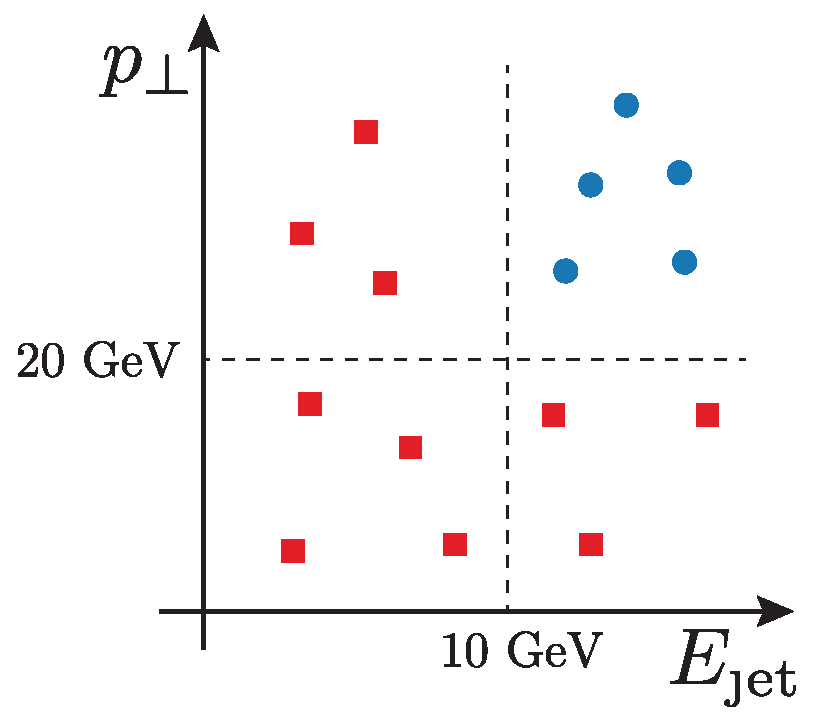
\includegraphics[width=\textwidth, trim=5 5 5 5, clip]{figures/decision_tree/tree_example.pdf}%     without .tex extension
  % or use \input{mytikz}
  \caption[Decision Tree Cuts In Feature Space]{Illustration of the cuts a decision tree model make for \textcolor{blue}{signal} in blue circles and \textcolor{red}{background} in red squares. This is a visualization in the feature space of the decision tree seen in Figure~\ref{fig:ml:decision_tree}.}
  \label{fig:ml:decision_tree_feature_space}
\end{marginfigure}

Decision trees (DTs) are simple machine learning methods that works by partitioning the feature space into smaller subspaces, high dimensional rectangles basically, and then fit each subspace with a constant (for regression problems) or a single label (for classification problems) \citep{hastieElementsStatisticalLearning2009}. 

A simple example of this is visualized in Figure~\ref{fig:ml:decision_tree_feature_space} and \ref{fig:ml:decision_tree}. Figure~\ref{fig:ml:decision_tree_feature_space} illustrates how the (hypothetical) signal and background distributions look in the 2D feature space. The dashed lines in the figure indicate the cuts made by the decision tree, cuts which are shown as a typical decision tree visualization in Figure~\ref{fig:ml:decision_tree}. 

\begin{figure}
  \centering
  \includestandalone[width=0.6\textwidth]{figures/decision_tree/decision_tree}%     without .tex extension
  % or use \input{mytikz}
  \caption[Decision Tree]{
    Illustration of a simple decision tree. Here the tree partitions the input feature space consisting of the two variables $p_\perp$ and $E_\mathrm{jet}$ into two categories; either signal or background. A visualization of the cuts in the feature space is shown in Figure~\ref{fig:ml:decision_tree_feature_space}.
  }
  \label{fig:ml:decision_tree}
\end{figure}
Here the top \q{box} is called the \emph{root} of the tree, any subsequent boxes are \emph{nodes}, except the final ones that are not split any further which are \emph{leaves}. At first, the decision tree partitions the space according to the value of the transverse momentum\sidenote{All units in this project are in natural units such that both momentum and energy are in units of \si{\eV}.} $p_\perp$: if it is lower than (or equal to) \SI{20}{\GeV} it classified as background. If the value is higher than \SI{20}{\GeV} an extra split is made. This split is on the energy of the jet $E_\mathrm{jet}$: if it is higher than \SI{10}{\GeV} it is classified as signal and otherwise as background. Training a decision tree on this data allows us to predict a new unseen event, $(p_\perp, E_\mathrm{jet}) = (\SI{24}{\GeV},\SI{11}{\GeV})$, to be a signal-like event. 

This decision tree is said to be a shallow tree since it only has a depth of \num{2}. The maximum depth allowed for the model is an important hyperparameter since it clearly controls under- and overfitting by changing how many cuts and partitions in the feature space are allowed; the deeper the tree, the more complex the model becomes. Single decision trees are very prone to overfitting
% \sidenote{With a solution to this problem given in \autoref{subsec:ml:multiple_decision_trees}.}
, however, they are also extremely inspectable. They are even referred to as \q{white-box models} compared to black-box models such as neural networks. For a more thorough introduction to decision trees and how they are internally optimized (for finding the best cut values), see \citet{hastieElementsStatisticalLearning2009}. 

\subsection{Ensembles of Decision Trees}
\label{subsec:ml:multiple_decision_trees}
Single decision trees are prone to overfitting and generally suffer from high variance. Today especially two different methods exist to alleviate these problems: random forests and boosted decision trees (BDTs). Both methods are examples of so-called ensemble methods where a set of ML methods are combined into a single model. Typically ensemble methods are based on \emph{weak learners}: simple, often fast, methods that individually show relatively poor generalization performance, typically due to high variance. 

\subsubsection{Random Forests}
\label{subsubsec:ml:random_forest}
Random forests were first introduced in 2001 by \citet{breimanRandomForests2001}. Random forests are collectiona of $B$ decision trees where each tree is trained on bootstrapped versions of the training data and then the individual trees' predictions $T_b$ are averaged\sidenote{In the case of classification it is the majority vote which is taken.}: 
\begin{equation}
  f_\mathrm{RF}(\vec{x}) = \frac{1}{B}  \sum_{b=1}^B T_b(\vec{x}).
\end{equation}
The method of making artificial extra samples and training on them is in general called bootstrap aggregation or \emph{bagging} \autocite{hastieElementsStatisticalLearning2009}. It works by averaging out noisy estimates of the individual models hence reducing variance. 
\begin{theorem}[Variance of average of correlated i.d. variables]
  Given $B$ identically distributed (but not necessarily independent) variables each with variance $\sigma^2$ and positive pairwise correlation $\rho$, the variance of the average is:
  \begin{equation}
    \label{eq:ml:variance_of_correlated_variables}
    \mathrm{Var}(\bar{\mu}_B) = \frac{1-\rho}{B} \sigma^2 + \rho \sigma^2,
  \end{equation}
  where $\bar{\mu}_B$ is the average of the i.d. variables \autocite{hastieElementsStatisticalLearning2009}. % XXX maybe write proof here myself: https://stats.stackexchange.com/questions/320083/calculating-the-variance-of-the-average-of-b-dependent-random-variable
\end{theorem}
Equation \eqref{eq:ml:variance_of_correlated_variables} is the main idea behind random forests. As the number of trees, $B$, in the forest increases, the first term goes towards zero. Thus, the more the correlation $\rho$ between the individual trees is reduced, the more the variance is reduced (which is the main problem in the case of decision trees to begin with). 

In addition to training the trees on bagged samples, one more technique is used to further decrease the correlation between the individual trees: each bootstrapped sample of the dataset not only contains just a subset of the observations (rows), but also only a subset of the variables (columns). This is called column subsampling (in contrast to row subsampling).

\marginnote[-2.5cm]{Throughout this project all data is assumed to be \emph{tidy data} unless otherwise explicitly mentioned. Tidy data was a concept formalized in 2003 by \citet{JSSv059i10} which basically states that each variable forms a column, each observation forms a row, and that each type of observation unit forms a table. This also means that the term variable and column will be used interchangeable (together with \emph{feature}), and likewise with observation and row.}

% Until very recently RF has suffered from the lack of a fast, optimized implementation in Python that could deal with big data sets. 

\subsubsection{Boosted Decision Trees}
\label{subsubsec:ml:boosted_decision_trees}
In the overall family of ensemble models, \emph{boosting} might be the most successful of them all where especially the specific algorithm called XGBoost \autocite{chenXGBoostScalableTree2016} revolutionized the ML world by winning numerous Kaggle\sidenote{Kaggle is an online platform where people compete with machine learning models.} competitions \autocite{DmlcXgboost} including the Higgs Machine Learning competition in \num{2014} \autocite{HEPMeetsML}. 

Boosting is the process of sequentially applying weak learner models to repeatedly modified versions of data \autocite{hastieElementsStatisticalLearning2009}. This combines many weak learners into a single strong learner in an iterative fashion. The final prediction is a weighted sum over the $K$ different weak learners $F_k$: 
\begin{equation}
  f_\mathrm{BDT}(\vec{x}) = F(\vec{x}) = \sum_{k=1}^K \alpha_k F_k(\vec{x})
\end{equation}
Boosting works by reducing both bias and variance since it iteratively fits weak learners. The variance is not reduced as much as for random forests since the weak learners are more correlated, however, their bias is lower. 

The term gradient boosting comes from the observation that repeatedly minimizing the residuals of the current model is similar to minimizing the gradient of the loss function for a specific choice of the loss function.
Imagine that we start off with an imperfect model $F_k(x)=\hat{y}$. In boosting, we want the next iteration to be a better model than the previous one, so imagine that the perfect addition to the model was $h(x)$. For it to be perfect, the following would have to be true:
\begin{equation}
  \label{eq:ml:boosted_decision_trees_residual}
  F_{k+1}(x) \equiv F_k(x) + h(x) = y \Leftrightarrow h(x) = y - F_k(x).
\end{equation}
The r.h.s. is the residual of the model, so at each stage the model is trying to fit the residuals of the current iteration of model. The \q{gradient} in \q{gradient boosting} comes from the following. Assume the loss function: $L(y, F_k(x)) = \frac{1}{2}  (y-F_k(x))^2$. The gradient of the loss w.r.t. $F_k(x)$ is:
\begin{equation}
  \frac{\partial L(y, F_k(x))}{\partial F_k(x)} = F_k(x) - y. 
\end{equation}
This is exactly the negative of the r.h.s. of equation \eqref{eq:ml:boosted_decision_trees_residual}. Instead of looking at the model as trying to minimize the residual at each iteration, it can instead be generalized as trying to fit the negative gradients of the loss function:
\begin{equation}
  h(x) = - \frac{\partial L}{\partial F_k}.
\end{equation}
We thus end up with the following iterative model which is basically a \emph{gradient descent} algorithm with the learning $\eta$ set to \num{1}:
\begin{equation}
  F_{k+1}(x) = F_k(x) + h(x) = F_k - \frac{\partial L}{\partial F_k}.
\end{equation}
When the learning rate is allowed to float, one gets:
\begin{equation}
  F_{k+1}(x) = F_k - \eta \cdot \frac{\partial L}{\partial F_k}.
\end{equation}
In general, the learning rate is a low value, e.g. $\eta=0.01$. The learning rate scales the following iteration by a factor $\eta$ after each step of tree boosting.

AdaBoost \autocite{freundDesiciontheoreticGeneralizationOnline1995} was the first major algorithm to make use of boosting. It was seen as a way of iteratively giving wrongly predicted observations higher weight, however, this is just a result of a \q{lucky} choice of loss function\sidenote{Exponential loss for classification.} which was not realized until much later. AdaBoost could be used with many different weak learners, however, mostly decision trees were used to form boosted decision trees. 

XGBoost \autocite{chenXGBoostScalableTree2016} is a fast, computationally efficient implementation of gradient boosting with decision trees as base learners: so-called \emph{boosted decision trees} (BDTs). It implements several model regularization techniques which makes it less prone to overfitting than other boosted decision trees. 

\section{Hyperparameter Optimization}
\label{sec:ml:hyperparameter_optimization}
By now, linear models with $L_1$ and $L_2$ regularization have been introduced along with decision trees, random forests and gradient boosted trees. All of these ML models tries to optimize their parameters according to some objective function. In addition to the parameters of the model, each one has a specific set of hyperparameters that cannot directly be optimized in the internal optimization process. This could be the amount of regularization $\lambda$ for linear models, the maximum tree depth for decision trees, the number of trees for random forests, or the column (or row) subsampling fraction for boosted decision trees. 

In general we say that we have the ML model $\mathcal{A}$ with $K$ hyperparameters. Each of these hyperparameters have a domain $\Lambda_k$. The domain can be either real numbers $\Lambda_k \in \mathbb{R}$, integers $\Lambda_k \in \mathbb{Z}$, binary $\Lambda_k \in \{0, 1\}$, or categorical\sidenote{Could e.g. be the choice of loss function.}. We define the hyperparameter configuration space as: $\bm{\Lambda} = \Lambda_1 \times \Lambda_2 \times \dots \times \Lambda_K$. Within this space we are searching for a vector of hyperparameters $\bm{\lambda} \in \bm{\Lambda}$ which defines the optimal model $\mathcal{A}_{\bm{\lambda}^*}$. Here the optimal model is the model which gives the best generalization performance according to some evaluation function. The goal of finding the best hyperparameter $\bm{\lambda^*}$ is known as \emph{hyperparameter optimization} (HPO).

The naive approach would simply be to manually\sidenote[][-5mm]{Also known jokingly as \q{Grad Student Descent}.} try out different combinations of $\bm{\lambda}$ and see performance on the validation set\sidenote{Remember only to use the test set on the final model.}. This is of course too cumbersome for advanced ML models, but it should be noted that it is a good place to start. In \autoref{subsec:ml:grid_search} the HPO method called grid search is introduced which is further generalized and optimized in \autoref{subsec:ml:random_search} with random search. Both these methods are easily parallelizable since they do not have any inherent history in its guesses. This is in contrast to Bayesian optimization introduced in \autoref{subsec:ml:bayesian_optimization} which allows for \q{smart} guesses.

\subsection{Grid Search}
\label{subsec:ml:grid_search}

Grid search (GS) is a HPO method also known as full factorial design. It is called grid search because it tries all possible combinations of the hyperparameter configuration space: the so-called cartesian product of $\bm{\Lambda}$. Imagine a 2D space where the two domains are respectively $x=\{1, 2, 3\}$ and $y=\{1, 2, 3,4\}$. Grid search runs through all $3 \times 4 = 12$ combinations of these two sets: 

\begin{marginfigure}[-4cm]
  \centerfloat
  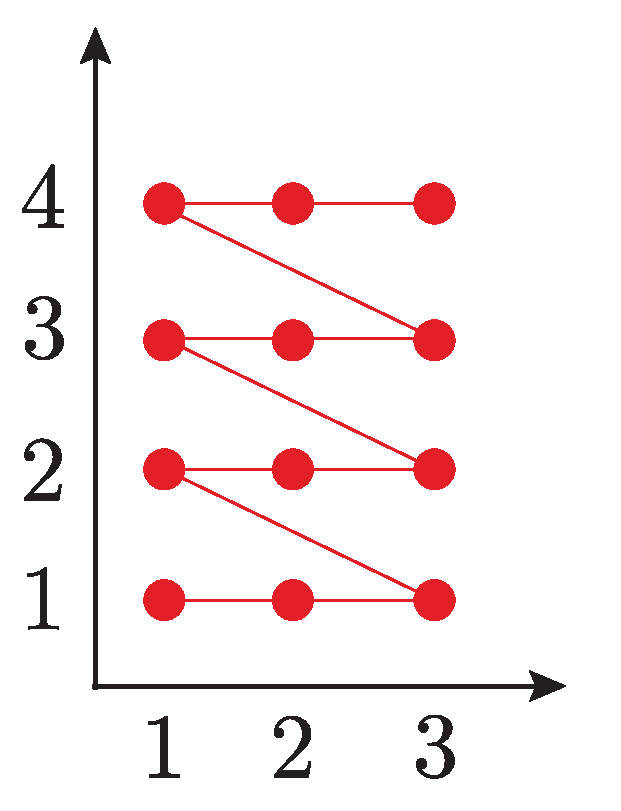
\includegraphics[width=\textwidth]{figures/gridsearch/grid.pdf}
  \caption[Grid Search]{Visualization of grid search run on the two hyperparameters $x$ and why $y$ with the domains $x=\{1, 2, 3\}$ and $y=\{1, 2, 3,4\}$.}
  \label{fig:ml:gridsearch}
\end{marginfigure}

\begin{equation}
  (x_i, y_i) \in \{(1, 1), (1, 2), \dots, (x_i, y_i), \dots, (3, 4)\},
\end{equation}
as visualized in Figure~\ref{fig:ml:gridsearch}. The advantage of grid search is that it is an exhaustive search over all combinations of hyperparameters, however, the total number of combinations grows exponentially and grid search as a method thus suffers the curse of dimensionality\sidenote{Not the dimensionality of the input feature space, but of the hyperparameter configuration space.}.



\subsection{Random Search}
\label{subsec:ml:random_search}

To circumvent the problems of grid search, \citet{bergstraRandomSearchHyperparameter2012} developed the Random Search (RS) algorithm in 2012. Regarding the effect of the curse of dimensionality on grid search they wrote: \emph{``This failure of grid search is the rule rather than the exception in high dimensional hyper-parameter optimization''} \citep{bergstraRandomSearchHyperparameter2012}. Instead of searching through all possible values of $\bm{\lambda}$, like in grid search, random search makes $B$ runs where each $\bm{\lambda}_i$ is given by:
\begin{equation}
  \label{eq:ml:random_search}
  \bm{\lambda}_i \sim \sum_{j=1}^K  \mathrm{PDF}_j(\Lambda_j) \cdot \bm{\hat{e}}_j ,
\end{equation}
where $\bm{\hat{e}}_j$ is the unit vector for dimension $j$ in the $K$ dimensional hyperspace. Equation \eqref{eq:ml:random_search} should be understood in the following way. For each hyperparameter draw a random number from a user-defined probability density function (PDF) and then let $\bm{\lambda}$ be the vector of those $K$ random numbers. In a 2D-space, $\bm{\lambda}_i$ could thus be: 
\begin{align}
  \bm{\lambda}_i \sim & \begin{bmatrix}
      \mathcal{N}(100, 4) \\
      \mathcal{U}(0, 1)
       \end{bmatrix},
\end{align}
where $\mathcal{N}(100, 4)$ is normal (Gaussian) distribution with mean $\mu=100$ and standard deviation $\sigma=4$ and $\mathcal{U}(0, 1)$ is the uniform distribution in the interval $[0, 1]$. The PDF can be a probability mass function (PMF) in the case of discrete hyperparameter domains.


The reason why random search is so powerful is not only because the number of function evaluations $B$ is easily tunable\sidenote{Compared to grid search which tries \emph{all} possible combinations.}, but also due to the fact that often some hyperparameter dimensions are more important than other. Even though the hyperparameter configuration space $\bm{\Lambda}$  might be high-dimensional, it often exhibits \emph{low effective dimensionality} \autocite{bergstraRandomSearchHyperparameter2012}. In the simplest 2D-case, this can be written as the following example. Imagine that we want to maximize some evaluation function, e.g. accuracy of the predictions, and the model depends on the two independent hyperparameters $x$ and $y$: $f(x, y)$. In this example assume that $f$ is almost insensitive to $y$ and thus has an effective dimensionality of 1. Then $f(x,y) = g(x) + h(y) \approx g(x)$. For a visualization of this example, see Figure~\ref{fig:ml:random_search}.

\begin{marginfigure}
  \centerfloat
  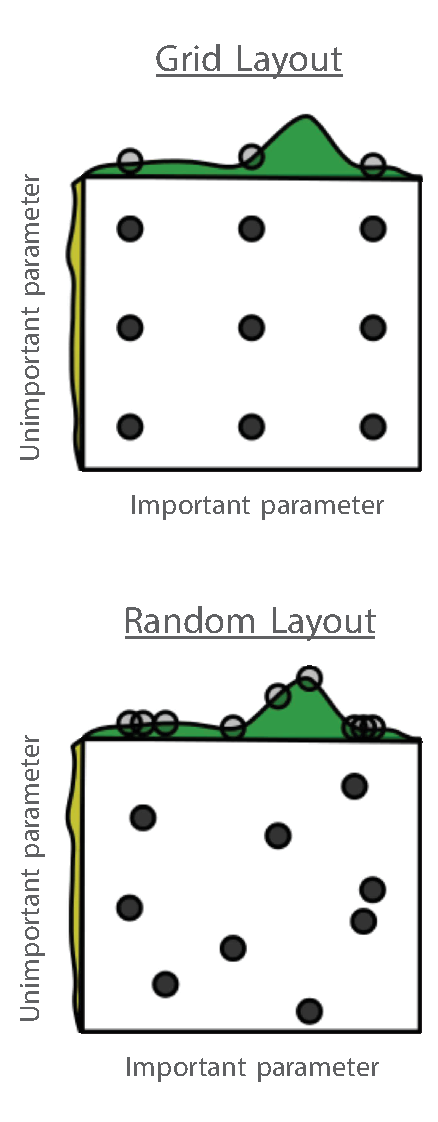
\includegraphics[width=1\textwidth]{figures/randomsearch/random.pdf}
  \caption[Random Search]{Visualization of the difference between grid search and random search. Adapted from \citet{bergstraRandomSearchHyperparameter2012}.}
  \label{fig:ml:random_search}
\end{marginfigure}

Grid search is run with a grid of $3\times3 = 9$ points in the figure and random search is similarly run with 9 points drawn from uniform PDFs in the same interval. It easy to see that when the hyperparameter configuration space has a lower effective dimensionality than the actual dimensionality, random search is far better at probing the space due to the projections into the sensitive dimensions cover more of these axes than for grid search. That the hyperparameter configuration space has lower effective dimension than its actual dimension is quite common. 

In general, only a fraction of all hyperparameters matter for any dataset but different hyperparameters matter in different datasets and thus generally random search performs as well as grid search or better \autocite{bergstraRandomSearchHyperparameter2012}. 
Note that random search can be seen as a generalization of grid search, where grid search is the specific example of random search if one uses a multidimensional binomial distribution as PDF and the PDF is reevaluated after each run. 

\subsection{Bayesian Optimization}
\label{subsec:ml:bayesian_optimization}
When performing hyperparameter optimization, it often takes a lot of time to evaluate the individual hyperparameters. Remember, that each evaluation consists of fitting $\mathcal{A}_{\bm{\lambda}}$ to the training data and then measure the performance on the validation set. Fitting the model on the training set can often take minutes, if not hours. This process is even slower when using cross validation. The idea behind Bayesian optimization is that when the ML model, or any other black box function, is expensive\sidenote{With respect to time.} to evaluate, then computing \q{smart} guesses are worth spending a bit of time. The hope is that the time taken to come up with smart guesses is negligible compared to the overall function evaluation time. This is contrast to both grid search and random search where each new set of hyperparameters $\bm{\lambda}$ are independent of the value of the evaluation performance.

In Bayesian optimization (BO) \autocite{brochuTutorialBayesianOptimization2010}, the evaluation function as a function of hyperparameter is assumed to be unknown. This unknown function is iteratively fitted with a probabilistic surrogate model, most often by Gaussian processes (GPs). Given the fitted surrogate model, an acquisition function is computed. This is a manually chosen function which is cheap to evaluate and is a measure of where in the high dimensional hyperparameter space the highest chance of finding a new good value of $\bm{\lambda}$ is. The acquisition function has to be chosen manually and especially the tradeoff between \emph{exploitation} versus \emph{exploration} is particularly important. This value decides how \q{adventurous} or conservative the BO algorithm should be when exploring the evaluation space. 

Bayesian optimization is better explained by looking at Figure~\ref{fig:ml:bayesian_optimization}. First look at the top plot. This is a plot of the surrogate function in black with uncertainties shown in blue. This is a result of fitting GPs to the two previous points, $t=2$. This surrogate function is supposed to fit the unknown hyperparameter-dependent evaluation function (called objective in the figure) shown as a dashed black line. Below we see the acquisition function in green. This is a function of the blue curve and the position of its maximum decides where the next guess of $\bm{\lambda}$ should be. With the chosen acquisition function and exploration willingness, we see that the next guess should be slightly to the left of the right-most point. This is a simple 1D toy problem, but one should imagine this happening in a high-dimensional space. After making a new guess, $t=3$ in the middle plot, the acquisition function changes since it learnt that this gave a worse evaluation value than the right-most point. Therefore, the next proposal for $\bm{\lambda}$ is slightly to the right of the right-most point. The process continues like this in an iterative fashion: first fitting GPs to the previous evaluation values and then choosing the next $\bm{\lambda}$ according the acquisition function. 

\begin{figure}
  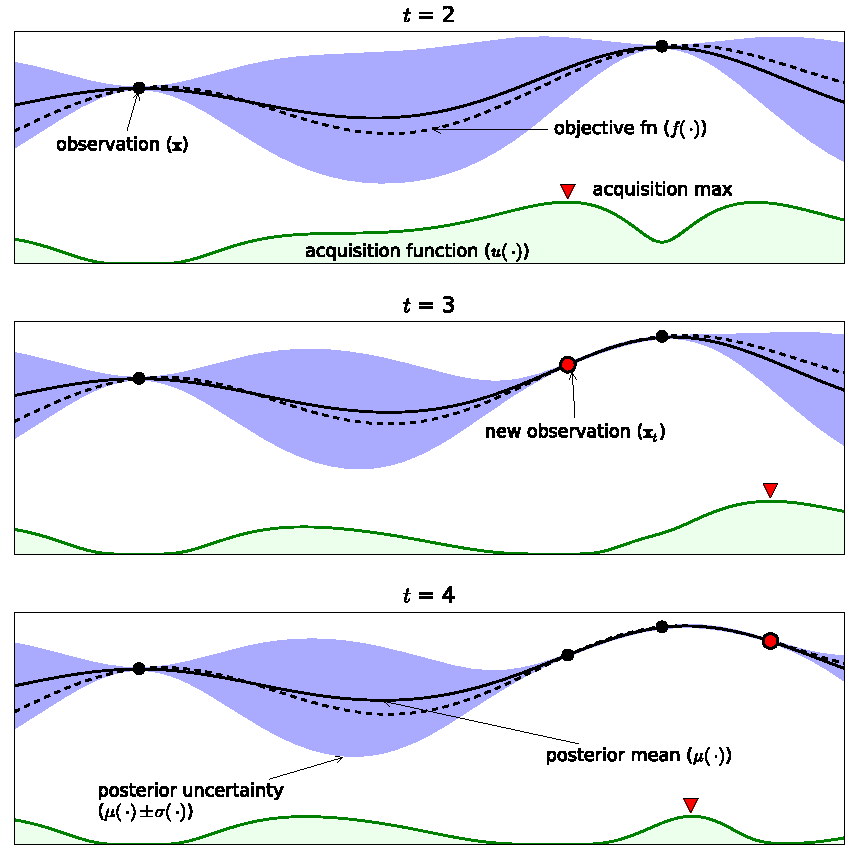
\includegraphics[width=0.99\textwidth]{figures/bayesian_optimization/bo_full.pdf}
  \caption[Bayesian Optimization]{Illustration of the learning process of Bayesian optimization. The previous observations are shown as black dots and the true objective function is shown as a dashed black line. This line is fitted with Gaussian processes (GPs) which is shown as the solid line with its uncertainty in purple. The acquisition function is shown in green and its maximum decides what the next iteration of the hyperparameter value(s) should be. 
  Adapted from \citet{brochuTutorialBayesianOptimization2010}.}
  \label{fig:ml:bayesian_optimization}
\end{figure}

Gaussian processes provide a posterior distribution given some prior distribution and the data-dependent likelihood. The process of BO is quite technical and mathematical, especially if GPs are new material. For a more in-depth explanation of the topic, see \citet{brochuTutorialBayesianOptimization2010}. The important thing to note is that GPs return not only a posterior mean $\mu(\vec{x})$ but also an uncertainty $\sigma(\vec{x})$, as seen in Figure~\ref{fig:ml:bayesian_optimization}. The acquisition function used in this project is the upper confidence bound (UCB):
\begin{equation}
  \mathrm{UCB}(\vec{x}) = \mu(\vec{x}) + \kappa \sigma(\vec{x}),
\end{equation}
where $\kappa \geq 0$ is the parameter\sidenote{Here $\kappa$ can be regarded as a hyper-hyperparameter since it controlls how the other hyperparamaters are optimized.} controlling the exploration exploitation tradeoff. 

Bayesian optimization has the great benefit of slowly learning the hyperparameter space and making smarter and more educated guesses over time. However, it also comes with the cost of being harder to numerically implement compared to grid search and random search\sidenote{Which are basically plug-and-play with Scikit-Learn \autocite{scikit-learn}.}, and parallelization is non-trivial to implement since it by definition is a sequential process. The performance boost is also not guaranteed. 

\section{Feature Importance}
\label{sec:ml:feature_importance}
Having first established that machine learning algorithms are indeed able to not only learn from data but also to generalize well without overfitting, modern ML hyperparameter optimized algorithms such as decision trees, random forests and boosted decision trees are generally performing well on very different data set. As such, one would think that machine learning has reached its goal. However, one of the most important issues in ML today is model inspection. Actually trying to make sense of the learnt model. Why does it predict as it does? Which features or variables are most important according to the model? Model interpretation is still very much active research today with no universally accepted methods. Some methods are model dependent and accurate, others might be model agnostic but slow or only approximations. In this project the focus will be on the so-called \emph{SHAP} values. 

In 2017, \citet{Lundberg:2017} showed that six different previously used methods were all specific instances of the same, universal underlying method and proposed SHaplay Additive exPlanation (SHAP) values as a unified measure of feature importance. In \num{2018} they developed a fast algorithm for computing SHAP values for tree ensemples and showed that previous measures of feature importance heavily used for trees, e.g. gain, were inconsistent \autocite{lundbergConsistentIndividualizedFeature2019}. That a measure for feature importance is inconsistent means that a model could rely more on feature $A$ than $B$, however, the feature importance would indicate opposite. SHAP values and permutation-based feature importances are both consistent feature importance measure, however, only SHAP allows for individualized\sidenote{Meaning that you can get the feature importances for a single observation compared to only the global, overall feature importances as seen across the entire data set.}, or local, feature importances.  

SHAP values are within the class of additive feature attribution methods, which are functions where the explanation model $g$ is a linear combination of binary variables \citep{Lundberg:2017}:
\begin{equation}
  \label{eq:ml:additive_feature_attribution_method}
  g(z') = \phi_0 + \sum_{i=1}^M \phi_i z_i'.
\end{equation}
Here $\phi_i \in \mathbb{R}$ are the feature importances and $z'$ is a binary variable such that $z_i'=1$ if the feature is present and otherwise $z_i' = 0$. SHAP values are based on Shapley regression values known from cooperative game theory \autocite{Shapley1953}. These values are based on the three axioms:
\begin{axiom}[Local Accuracy]
  Local accuracy says that the sum of the feature importances should equal the total reward:
  \begin{equation}
    f(x) = g(z') = \phi_0 + \sum_{i=1}^M \phi_i z_i'.
  \end{equation}
\end{axiom}
Here $f$ is the ML model, $g$ is the explanation model, $x$ is an observation in input feature space, $z'$ is an observation in the binary space as described above, and $\phi_i$ is the feature importance. 
\begin{axiom}[Missingness]
  Missingness means that features missing in the original input feature space (such that $z_i'=0$) should be attributed no importance:
  \begin{equation}
    z_i' = 0 \Rightarrow \phi_i = 0.
  \end{equation} 
\end{axiom}
\begin{axiom}[Consistency]
  \label{axiom:ml:shap_consistency}
  Consistency states if a model is changed such that it relies more on a certain feature, the feature importance of that feature should never decrease. 
\end{axiom}
% \begin{description}
%   \item[Local Accuracy] 
%   Local accuracy says that the sum of the feature importances should equal the total reward:
%   \begin{equation}
%     f(x) = g(x') = \phi_0 + \sum_{i=1}^N \phi_i x_i'.
%   \end{equation}
%   Here $f$ is the ML model, $g$ is the explanation model, $x$ is an observation in input feature space, $x'$ is an observation in the binary space as described above, and $\phi_i$ is the feature importance. 

%   \item[Missingness] Missingness means that features missing in the original input feature space (such that $x_i'=0$) should be attributed no importance:
%   \begin{equation}
%     x_i = 0 \Rightarrow \phi_i = 0
%   \end{equation}
%   \item[Consistency] Consistency states if a model is changed such that it relies more on a certain feature, the feature importance of that feature should never decrease.
% \end{description}
Given these three axioms, \citet{Lundberg:2017} show that the only solution to equation \eqref{eq:ml:additive_feature_attribution_method} is:
\begin{equation}
  \label{eq:ml:shap_feature_importance}
    \phi_i = \sum_{S \subseteq \widetilde{M} \backslash \{i\}} \frac{|S|!(M-|S|-1)!}{M!} \left[ f_x(S \cup \{i\}) - f_x(S) \right] ,
\end{equation}
which one can rewrite to:
\begin{equation}
  \label{eq:ml:shap_feature_importance_simplification}
  \begin{split}
    \phi_i        &= \sum_{S \subseteq \widetilde{M} \backslash \{i\}} w(S) \cdot \Delta_{f_x}(S) \\
    w(S)             &\equiv \frac{|S|!(M-|S|-1)!}{M!} \\
    \Delta_{f_x}(S)  &\equiv \left[ f_x(S \cup \{i\}) - f_x(S) \right].
  \end{split}
\end{equation}


In equation \eqref{eq:ml:shap_feature_importance} $\widetilde{M}$ is the \emph{set} of all input features\sidenote{Compared to $M=|\widetilde{M}|$ which is the \emph{number} of all input features.}, $S \subseteq \widetilde{M} \backslash \{i\}$ means a subset $S$ of $\widetilde{M}$ without feature $i$, $S \cup \{i\}$ means the set $S$ with feature $i$ and $f_x(S) = f(h_x(z'))$ where $h_x(z')$ is the mapping function from the binary $z'$ space to the input feature space $x$. In equation \eqref{eq:ml:shap_feature_importance_simplification} the function is simplified to its basic constituents: the difference in performance  between including feature $i$ and not including it, $\Delta_{f_x}$, and its weight $w$. 

To get a better understanding of the different terms in equation \eqref{eq:ml:shap_feature_importance_simplification}, one could look at the decision tree shown in Figure~\ref{fig:ml:decision_tree}. Here $\widetilde{M}$ would be $\widetilde{M}=\{p_\perp, E_\mathrm{jet} \}$. For the feature $i=p_\perp $ one would thus have:
\begin{equation}
  \begin{split}
    \phi_{p_\perp} = & \sum_{S \subseteq \widetilde{M} \backslash \{p_\perp \}} w(S)  \cdot\Delta_{f_x}(S)  \\
                   = & \sum_{S \in \left[\{\}, \{E_\mathrm{jet}\} \right]} w(S)  \cdot\Delta_{f_x}(S)  \\
                   = & \frac{0! (2-0-1)!}{2!} \cdot [ f_x(\{p_\perp\}) - f_x(\{\})]  \\ 
                     & +    \frac{1! (2-1-1)!}{2!} \cdot [f_x(\{ E_\mathrm{jet}, p_\perp \}) - f_x(\{ E_\mathrm{jet} \})].
  \end{split}
\end{equation}
Whereas $w(S)$ is easily calculated, $\Delta_{f_x}$ depends on the data and the ML model. As the number of features grows, the number of terms in the sum grows exponentially. What \citet{lundbergConsistentIndividualizedFeature2019} did was to develop an efficient algorithm that could solve this in polynomial time for trees\sidenote{Specifically they managed to improve the time complexity from $\mathcal{O}(TL2^M)$ to $\mathcal{O}(TLD^2)$ where $T$ is the number of trees, $L$ is the maximum number of leaves in any tree, $M$ is the number of features, and $D$ is the maximum depth of any tree (where $D\approx \log L$ for balanced trees).}. 

SHAP values allow one to explain for a single observation why it got the prediction that it got. When applied to the entire data set $\vec{X} \in \mathbb{R}^{N \times M}$ with $N$ observations each with $M$ features, one gets the matrix $\bm{\Phi} \in \mathbb{R}^{N \times M}$. When summing over the absolute value of each column, one gets the global impact $\phi_i^\mathrm{tot}$ of the $i^{\mathrm{th}}$ feature \citep{lundbergConsistentIndividualizedFeature2019}:
\begin{equation}
  \phi_i^\mathrm{tot} = \sum_{j=1}^N \abs{ \bm{\Phi}_{i, j} }.
\end{equation}
The global feature importance $\phi_i^\mathrm{tot}$ is thus a measure of the overall importance of feature $i$. 

Note that if one introduces a new feature to the dataset correlated\sidenote{Not necessarily linearly correlated.} to an already existing feature, the feature importance of the previous feature will decrease. 
This is due to the axiom of symmetry:
\begin{axiom}[Symmetry]
  \label{axiom:ml:shapley_symmetry}
  If for all subsets S that do not contain $i$ or $j$: 
  \begin{equation}
    f_x(S \cup \{i\}) = f_x(S \cup \{j\})
  \end{equation}
  then $\phi_i = \phi_j$.
\end{axiom}
It can be shown that axiom \ref{axiom:ml:shapley_symmetry} is implied by axiom \ref{axiom:ml:shap_consistency}  \citep[Supp. Material]{Lundberg:2017}. Two identical features, as seen by the model, will thus \q{share} the feature importance.


\chapter{Danish Housing Prices}
\label{ch:housing_price_analysis}
\epigraph{\textit{``Buy land, they’re not making it anymore.''}}{--- Mark Twain}
% \epigraph{\textit{``It’s tangible, it’s solid, it’s beautiful. It’s artistic, from my standpoint, and I just love real estate.''}}{--- Donald Trump}
\newthought{Housing markets} have always been a playing field for economists, property speculators, real estate agents, and realtors. Personally, I am by no metric any of these, not even close to. Yet, the issue of estimating housing prices purely on a data driven basis was too interesting to ignore. Estimating housing prices is a classical economical discipline as seen in papers from the Danish National Bank developing a regional model of the Danish housing market \autocite{hviidWorkingPaperRegional2017} to an analysis of the financial crisis in \num{2008}-\num{2009} and its effects on the Copenhagen metropolitan area \autocite{mulalicFinancialCrisisDiverging2017}. 

\begin{figure*}
  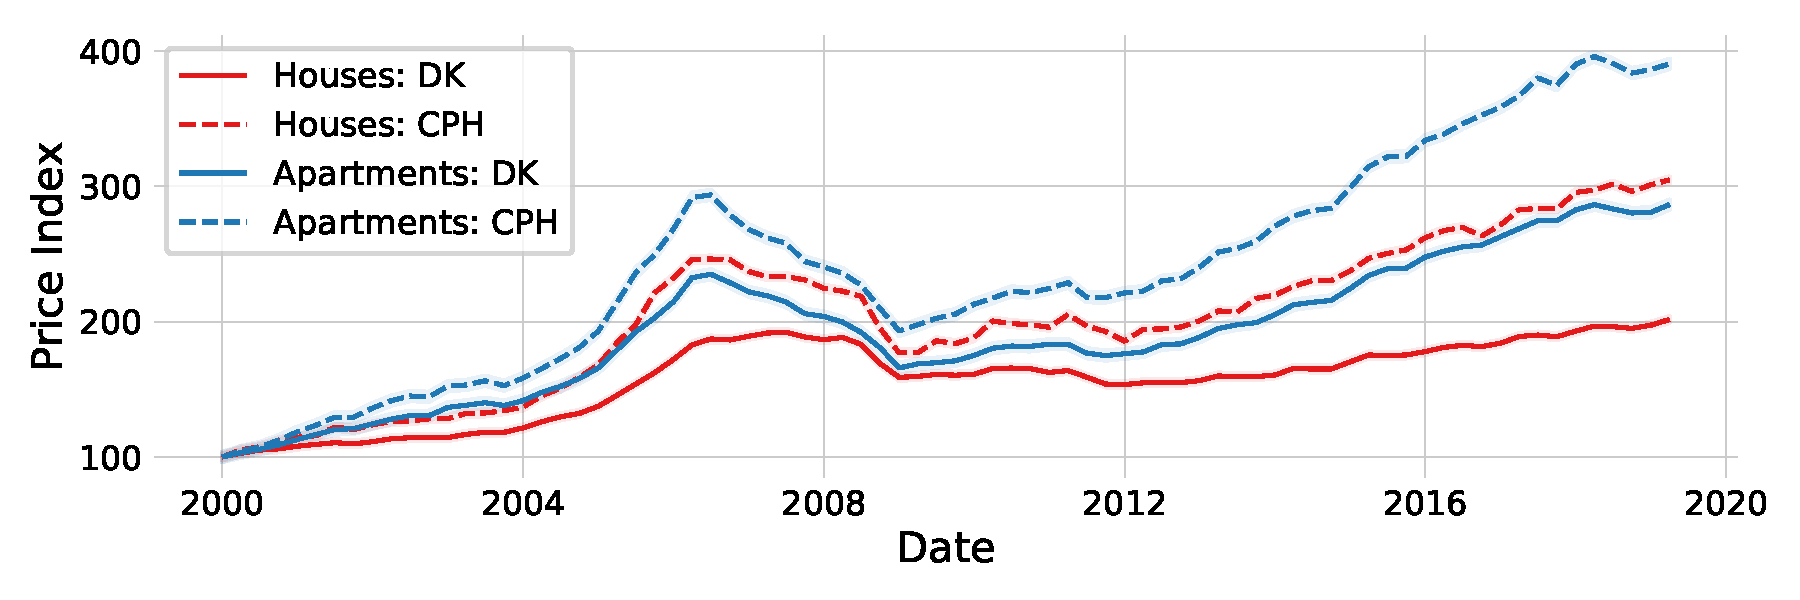
\includegraphics[width=0.98\textwidth, trim=10 15 10 10, clip]{figures/housing_price_index_dst/housingindex_wide.pdf}
  \caption[Price Index of the Danish Housing Market]
          {Prince index of Danish one-family houses and owner-occupied apartments where \textcolor{red}{houses} are shown in red and \textcolor{blue}{apartments} in blue, where full lines are for the entirety of Denmark and dashed lines are only for Copenhagen. Errorbars (scaled up with a factor of 2) are shown as colored bands. The price index and its uncertainty is based on numbers from \citet{dstPriceIndexEJ14}, however, rescaled to 100 in 2000 (instead of 2006 as it was in the data).}
  \label{fig:h:price_index}
\end{figure*}

If one takes a look at the time development of the Danish housing market, the Danish governmental organization for statistics, Statistics Denmark, releases a price index \citep{dstPriceIndexEJ14} for both one-family houses (OFH) and owner-occupied apartments (OOA) quarterly, see Figure~\ref{fig:h:price_index}. Here it is easy to see the effect of the financial crisis around 2008, but also the steady increase in the housing market in both Copenhagen and the entire country since then. Housing in this context means both actual houses and privately owned apartments, and will be called residences in general in this project. 

The goal of this subproject is not to predict any future collapse in the financial markets as we saw upwards of 10 years ago. Instead, it is to learn patterns in the price of houses in steady times. The goal is training a computer to automatically\sidenote{In contrary to \citet{hviidWorkingPaperRegional2017, mulalicFinancialCrisisDiverging2017} and others who base their models on macro-economic principles.} be able to find these patterns and see if we can improve this model.

This chapter is organized as follows. The data will be introduced in  \autoref{sec:h:data_cleaning} where also some initial plots are shown. The data set is feature augmented in \autoref{sec:h:feature_augmentation} and the different evaluation functions will be discussed in \autoref{sec:h:evaluation_function}. The choice of evaluation function will be based on an initial hyperparameter optimization process in \autoref{sec:h:initial_hyperparameter_optimization}. The model is fitted and optimized in \autoref{sec:h:hyperparamater_optimization} and the results from the final model are presented in \autoref{sec:h:results}. The forecasting performance of the model will be tested in \autoref{sec:h:forecasting}. To better understand the model, \autoref{sec:h:model_inspection} deals with the issue of model inspection. The model is extended by combining multiple ML models into an ensemble, a process that is described in \autoref{sec:h:multiple_models}. Finally, the project concerning Danish housing prices will be discussed in \autoref{sec:h:discussion} and concluded in \autoref{sec:h:conclusion}.

\section{Data Preparation and Exploratory Data Analysis}
\label{sec:h:data_cleaning}
\epigraph{\textit{``\SI{80}{\percent} of data science is cleaning the data and \SI{20}{\percent} is complaining about cleaning the data.''}}{--- Anthony Goldbloom, Kaggle}


The first part of any data science project is actually getting the data and being able to read it. This has been an iterative process that has improved over time. The last data transfer we got was September \nth{3} 2019 which consisted of a \SI{522.4}{\mega\byte} CSV file with dimensions $(\num{711212}, \num{171})$. This section will go through the data cleaning process.

Before any further data analysis is performed, all of the data is loaded, except columns which only contain internal information for Boligsiden\sidenote[][-1cm]{The variables \code{Sag_Kvhx}, \code{Bygning_GOP_Matrikelnr}, and \code{Enhed_GOP_BoligtypeKode}.}. To get a better understanding of all the original input variables, histograms of the one-dimensional distributions of each variable are shown in Figures\sidenote[][-5mm]{Where the A indicates that the figures are in the the \hyperref[appendix:housing]{appendix}.}~\ref{fig:h:variable_overview_all_1} to \ref{fig:h:variable_overview_all_14}.

Four particularly interesting distributions are shown in Figure~\ref{fig:h:variable_overview}: the date of the sale \code{SalgsDato} in subfigure~\subref{fig:h:variable_overview_date}, the type of residence \code{SagtypeNr} in subfigure~\subref{fig:h:variable_overview_type},
the longitude of the residence \code{GisX_WGS84} in subfigure~\subref{fig:h:variable_overview_longitude}, and the area of the residence \code{ArealBolig} in subfigure~\subref{fig:h:variable_overview_area}.

\begin{margintable}[0.5cm]
  \centering
  \begin{tabular}{@{}rl@{}}
  % \toprule
  Code & Name           \\ 
  \midrule
  100  & Villa          \\ 
  200  & Rækkehus       \\
  300  & Ejerlejlighed  \\
  400  & Fritidsbolig   \\
  401  & Kolonihave     \\
  500  & Andelsbolig    \\
  600  & Landejendom    \\
  700  & Helårsgrund    \\
  800  & Fritidsgrund   \\
  900  & Villalejlighed \\
  1000 & Kvæggård       \\
  1100 & Svinegård      \\
  1200 & Planteavlsgård \\
  1300 & Skovejendom    \\
  1400 & Lystejendom    \\
  1500 & Specialejendom \\ 
  % \bottomrule
  \end{tabular}
  \vspace{2mm}
  \caption[Mapping between the Code in \code{SagTypeNr} and the Type of Residence]{Mapping between the code in \code{SagTypeNr} and the type of residence. The two important types of residences are \q{villa} (one-family houses) and \q{ejerlejlighed} (owner-occupied apartments).}
  \label{tab:h:salgstype}
\end{margintable}

The distribution of the date of sale, Figure~\ref{fig:h:variable_overview} \subref{fig:h:variable_overview_date}, is an interesting variable because it shows how Boligsiden has been collecting more and more data over time. Here \num{2007} and \num{2019} are clear outliers since their current database only contains sales from the end of \num{2007}, and \num{2019} only contains data from the first eight months of the year. The \code{SagTypeNr} is a discrete code that Boligsiden uses to differentiate between different types of residences. The mapping between code and description is shown in Table~\ref{tab:h:salgstype}. 

\begin{figure*}
  \centering
  \subfloat[\label{fig:h:variable_overview_date}]{\qquad}
  \includegraphics[width=0.45\textwidth, page=2, trim=15 15 15 15, clip]{figures/housing/overview_fig.pdf}\hfil
  \subfloat[\label{fig:h:variable_overview_type}]{\qquad}
  \includegraphics[width=0.45\textwidth, page=6, trim=15 15 15 15, clip]{figures/housing/overview_fig.pdf}
  \subfloat[\label{fig:h:variable_overview_longitude}]{\qquad}
  \includegraphics[width=0.45\textwidth, page=20, trim=15 15 15 15, clip]{figures/housing/overview_fig.pdf}\hfil
  \subfloat[\label{fig:h:variable_overview_area}]{\qquad}
  \includegraphics[width=0.45\textwidth, page=23, trim=15 15 15 15, clip]{figures/housing/overview_fig.pdf}
  \caption[Distributions of the Variables in the Housing Prices]{Distributions of four out of the \num{168} input variables. 
           Subplot ~\protect\subref{fig:h:variable_overview_date} shows the date of the sale, 
           Subplot ~\protect\subref{fig:h:variable_overview_type} shows the type of residence,
           Subplot ~\protect\subref{fig:h:variable_overview_longitude} shows the longitude,
           Subplot ~\protect\subref{fig:h:variable_overview_area} shows the area of the house.}
  \label{fig:h:variable_overview}
\end{figure*}

% \vspace{-2cm}
In this project only one-family houses (\q{Villas}) with code \num{100} and owner-occupied apartments (\q{Ejerlejlighed}) with code \num{300} are considered. In Figure~\ref{fig:h:variable_overview} \subref{fig:h:variable_overview_type} it is shown that these two types of residences are also the most frequent sales with close to \num{400000} and \num{150000} sales in total. The longitude distribution, Figure~\ref{fig:h:variable_overview} \subref{fig:h:variable_overview_longitude}, is mostly interesting due to fact that it clearly shows how the Great Belt and especially the Baltic Sea separates Denmark into three parts; the Western part, the Eastern part, and then Bornholm. Note that more than \SI{5}{\percent} of the residences' locations are unknown values, so-called \q{Not A Number}s (NANs). The distribution of the area, Figure~\ref{fig:h:variable_overview} \subref{fig:h:variable_overview_area}, shows that most residences are between \SI{50}{\meter^2} and \SI{200}{\meter^2}, as expected in Denmark. However, a relatively large part of the residences, \SI{2.5}{\percent}, are listed as having an area of \SI{0}{\meter^2} which are obviously erroneous entries.

\begin{figure*}
  \centering
  \subfloat[\label{fig:h:geo_overview_sqm_price}]{\,}
  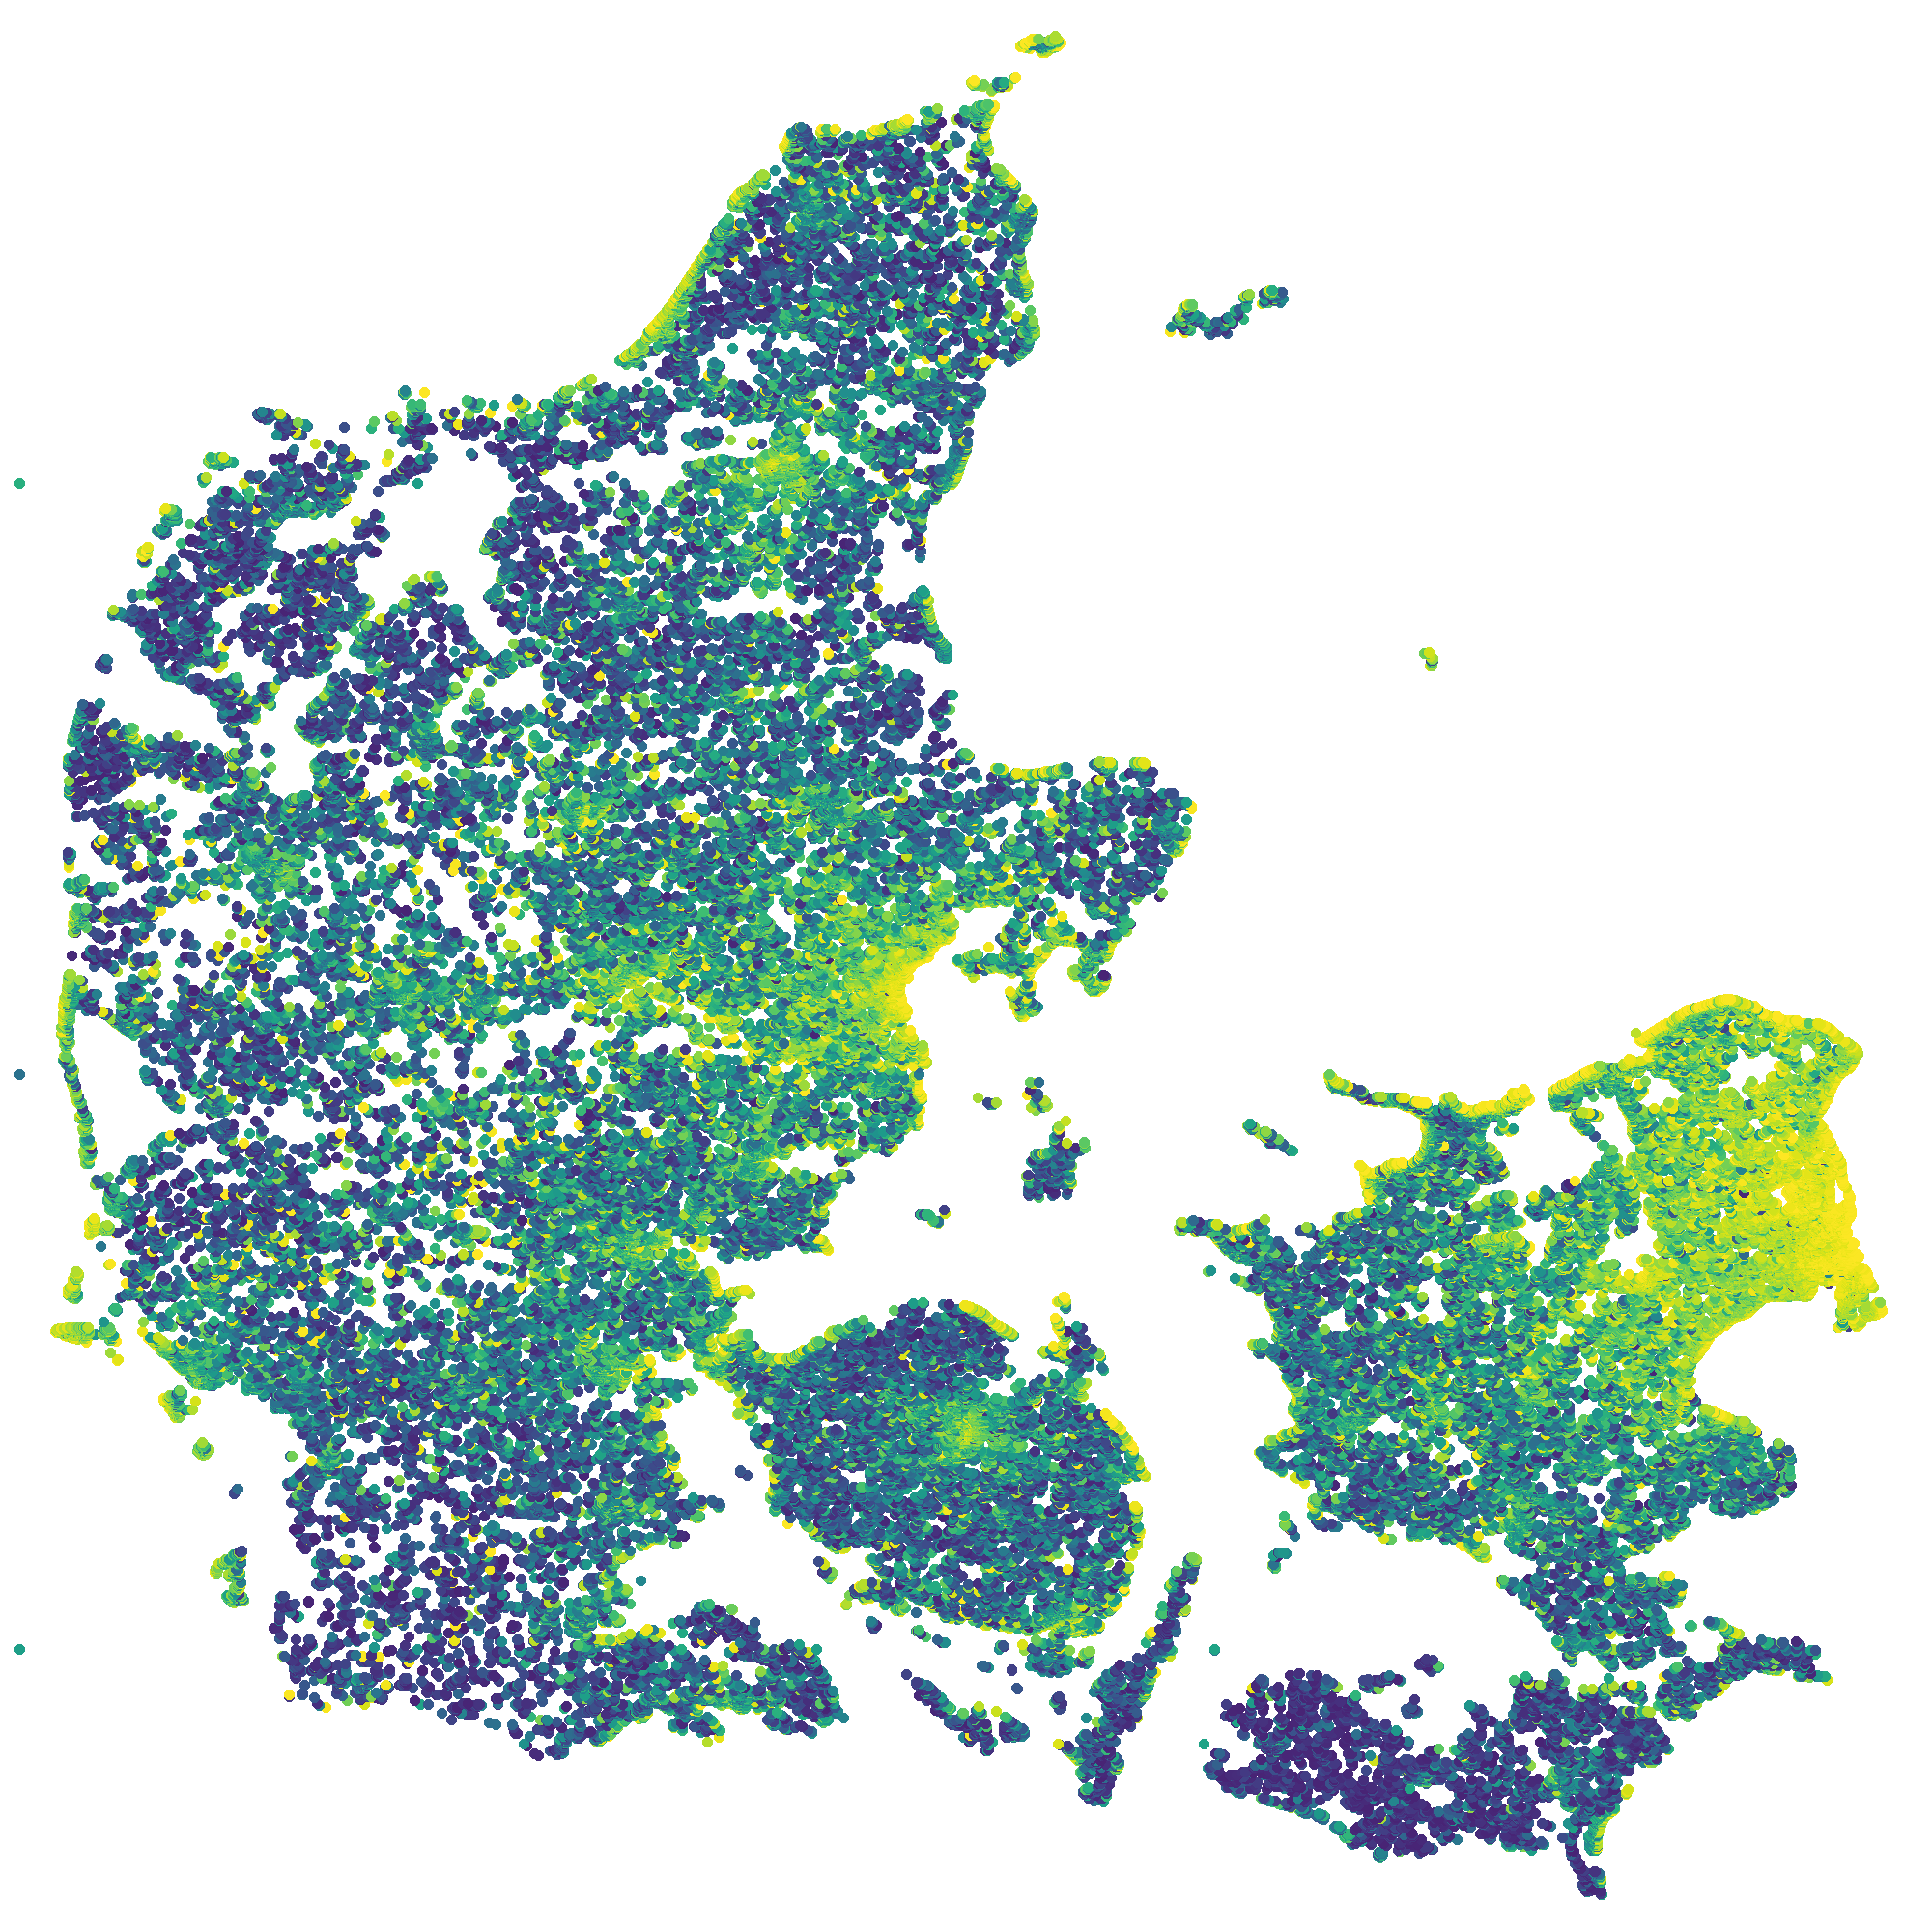
\includegraphics[draft=false, width=0.4\textwidth]{figures/housing/Denmark_Overview_SqmPrice.png}\hfil
  \subfloat[\label{fig:h:geo_overview_sales_price}]{\,}
  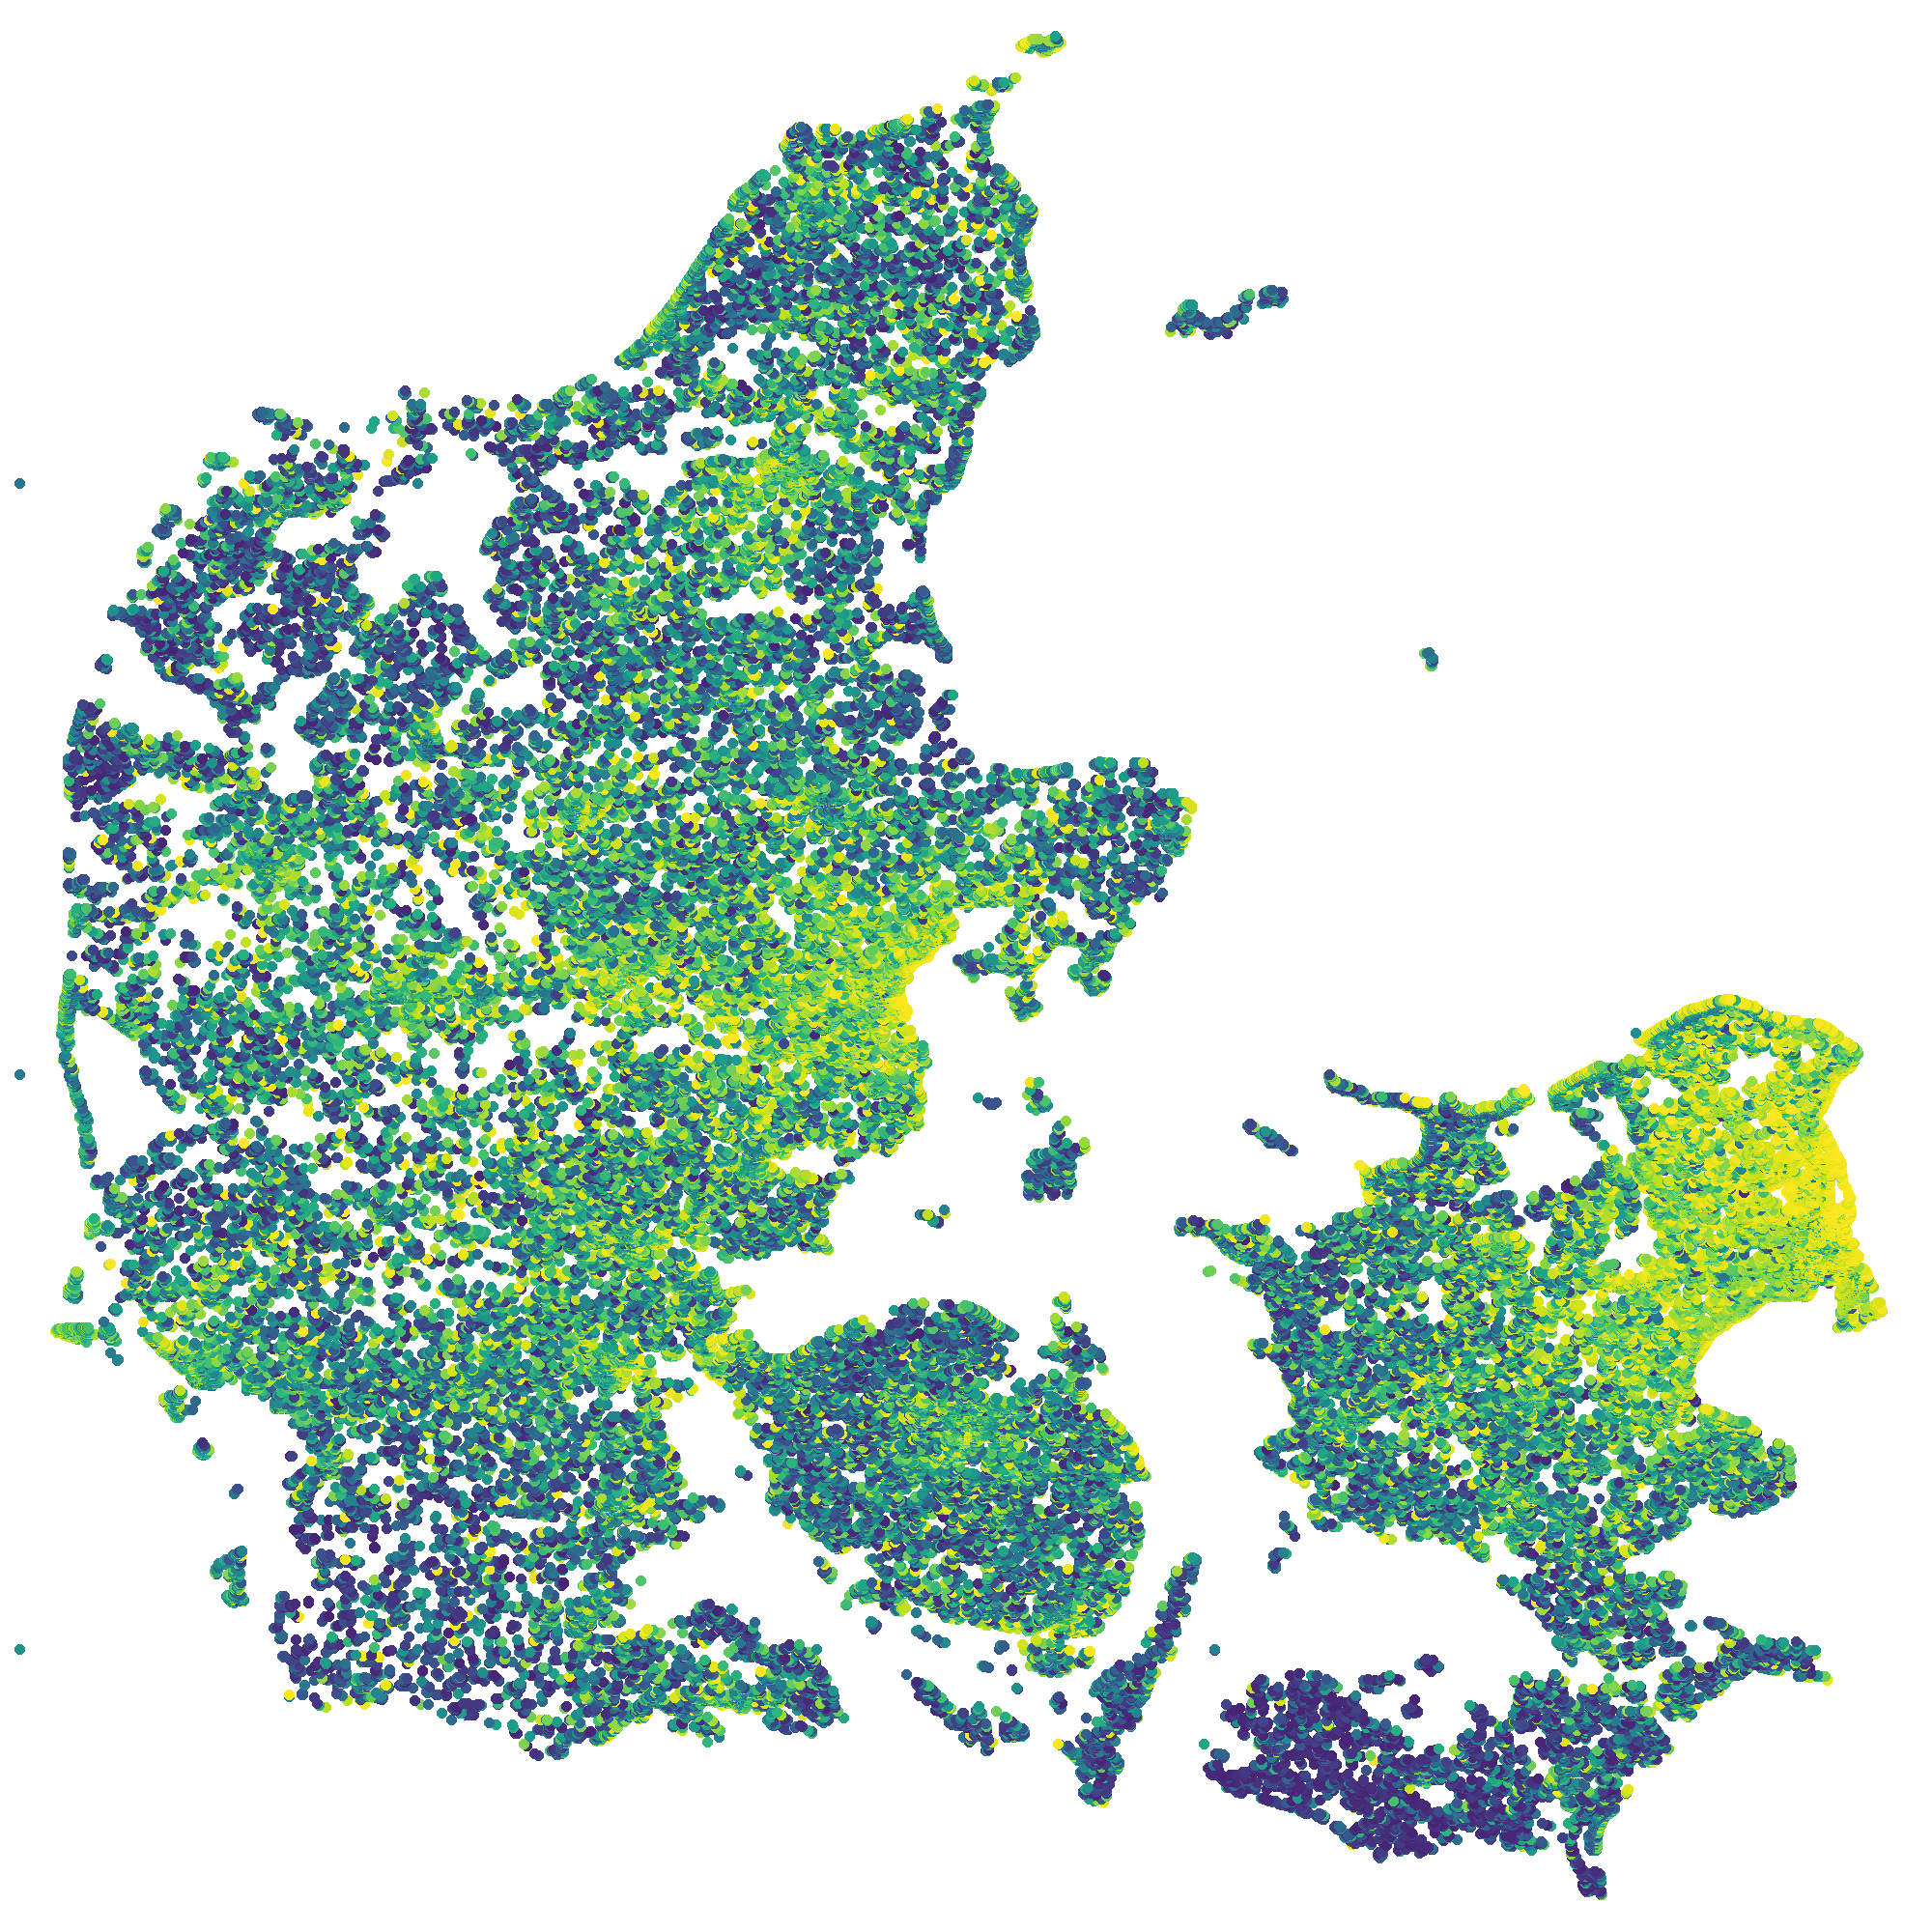
\includegraphics[draft=false, width=0.4\textwidth]{figures/housing/Denmark_Overview_SalesPrice.png}
  \caption[Geographic Distribution of the Sold Residences]{Geographic distribution of the sold residences. 
           In subplot ~\protect\subref{fig:h:geo_overview_sqm_price} the sales are colored according to their square meter price and in subplot ~\protect\subref{fig:h:geo_overview_sales_price} according to the sales price. 
           }
  \label{fig:h:geo_overview}
\end{figure*}

The geographic distribution of sales are shown in Figure~\ref{fig:h:geo_overview}. The residences are coloured according to the square meter price in Figure~\ref{fig:h:geo_overview} \subref{fig:h:geo_overview_sqm_price} and according to the sales price in Figure~\ref{fig:h:geo_overview} \subref{fig:h:geo_overview_sales_price}. Notice the strong correlation between the distance to water and the square meter price, a correlation that is less visible when looking at the sales price. Since these plots each contain \num{674647} points\sidenote{Only sales with a valid GPS-coordinate and area of residence are shown}, over-plotting quickly becomes an issue. To circumvent this, the software package called DataShader \autocite{bednarDatashaderRevealingStructure2019} was used which in a simple, consistent, and not at least computationally efficient manner allows one to plot big data.



The most important of the features is the sales price, called \code{SalgsPris} in the dataset. Its distribution is shown in Figure~\ref{fig:h:price_overview_price}. This is a positively skewed distribution that shares visual similarities with a log-normal distribution. The mode of the all sales prices\sidenote{Measured in millions DKK, \si{\Mkr}} is \SI{1.1}{\Mkr} and the median is \SI{1.6}{\Mkr} The mean is \SI{2.0}{\Mkr} but this value is heavily influenced by a few very high values. 

\begin{figure}
  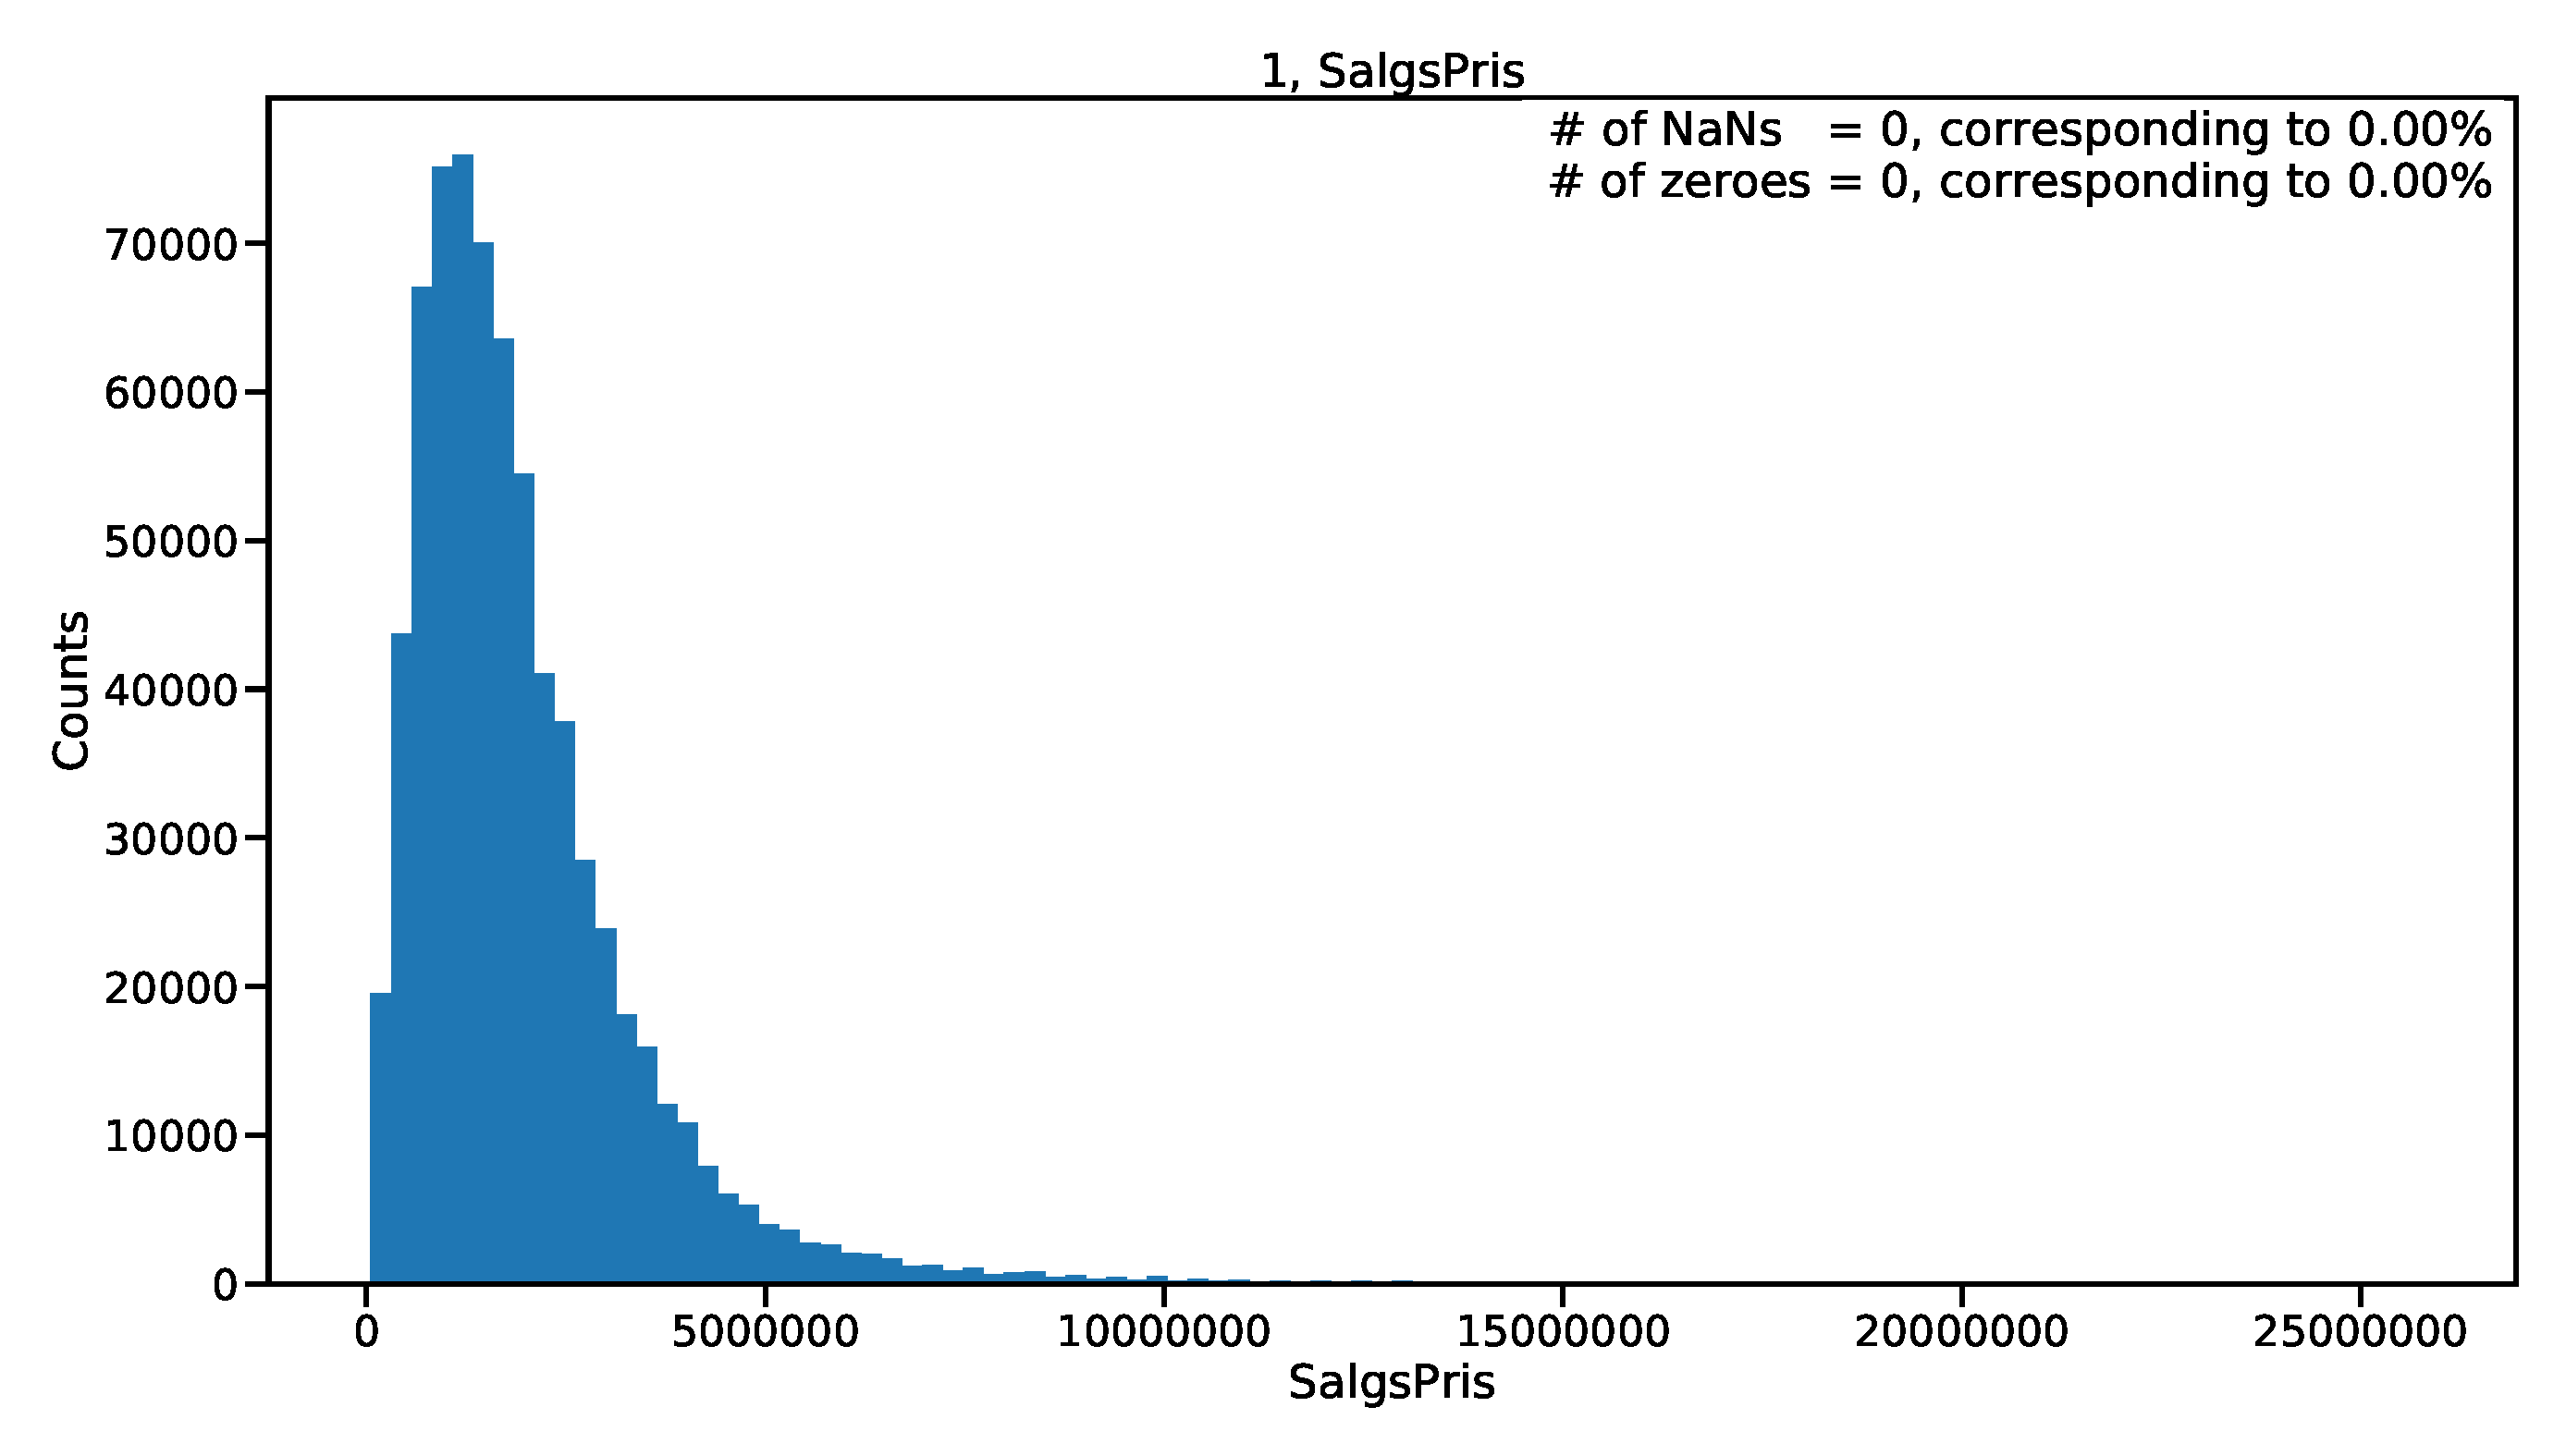
\includegraphics[width=0.98\textwidth, page=1, trim=15 15 15 15, clip]{figures/housing/overview_fig.pdf}
  \caption[Histogram of Prices of Houses and Apartments Sold in Denmark]
          {Histogram of prices of houses and apartments sold in Denmark.}
  \label{fig:h:price_overview_price}
\end{figure}

\vspace{-0.5cm}
\subsection{Correlations}
\label{subsec:h:correlations_lin_mic}

Having shown the \num{1}D-distributions of all the different variables in the previous section, the next step would be to look at the correlations between the variables. Since there are \num{168} input variables, it is almost impossible to understand every inter-variable correlation, however, it is tried in Figure~\ref{fig:h:correlations_all_lin}. In this figure, the correlations $\rho$ between all numerical variables that are not obviously related to other variables (like the GPS-coordinates that are in both latitude-longitude and ETRS89\sidenote[][-5mm]{European Terrestrial Reference System \num{1989}.} format), are plotted as a $(86 \times 86)$-dimensional heatmap\sidenote{With the condition that each plotted variable has to have at least one inter-variable correlation higher than $|\rho| > \SI{30}{\percent}$}.

Even though inter-variable correlations are important in the exploratory data analysis (EDA) phase, what is more important is to get a better understanding of how the input variables correlate with the output variable; the sales price. This is shown in Figure~\ref{fig:h:corr_lin} for the variables where $\abs{\rho} > \SI{10}{\percent}$. It is the previous property evaluation, \code{EjdVurdering_EjendomsVaerdi} that is correlated the most with the sales price, which does not come as any huge surprise. Other positively correlated variables are the cost of ownership\sidenote{This a great example of the fact that correlation does not imply causation as simply increasing the cost of ownership does not increase the sales price.}, area, number of bathrooms, longitude, and distance to nearest wind mill. In the other end, the local income tax, \code{Kommune_SkatteProcent}, is the variable that is the most negatively correlated to the sales price, followed by the geographical variables related to province, municipality, and postcode.

\begin{figure*}
  \centerfloat
  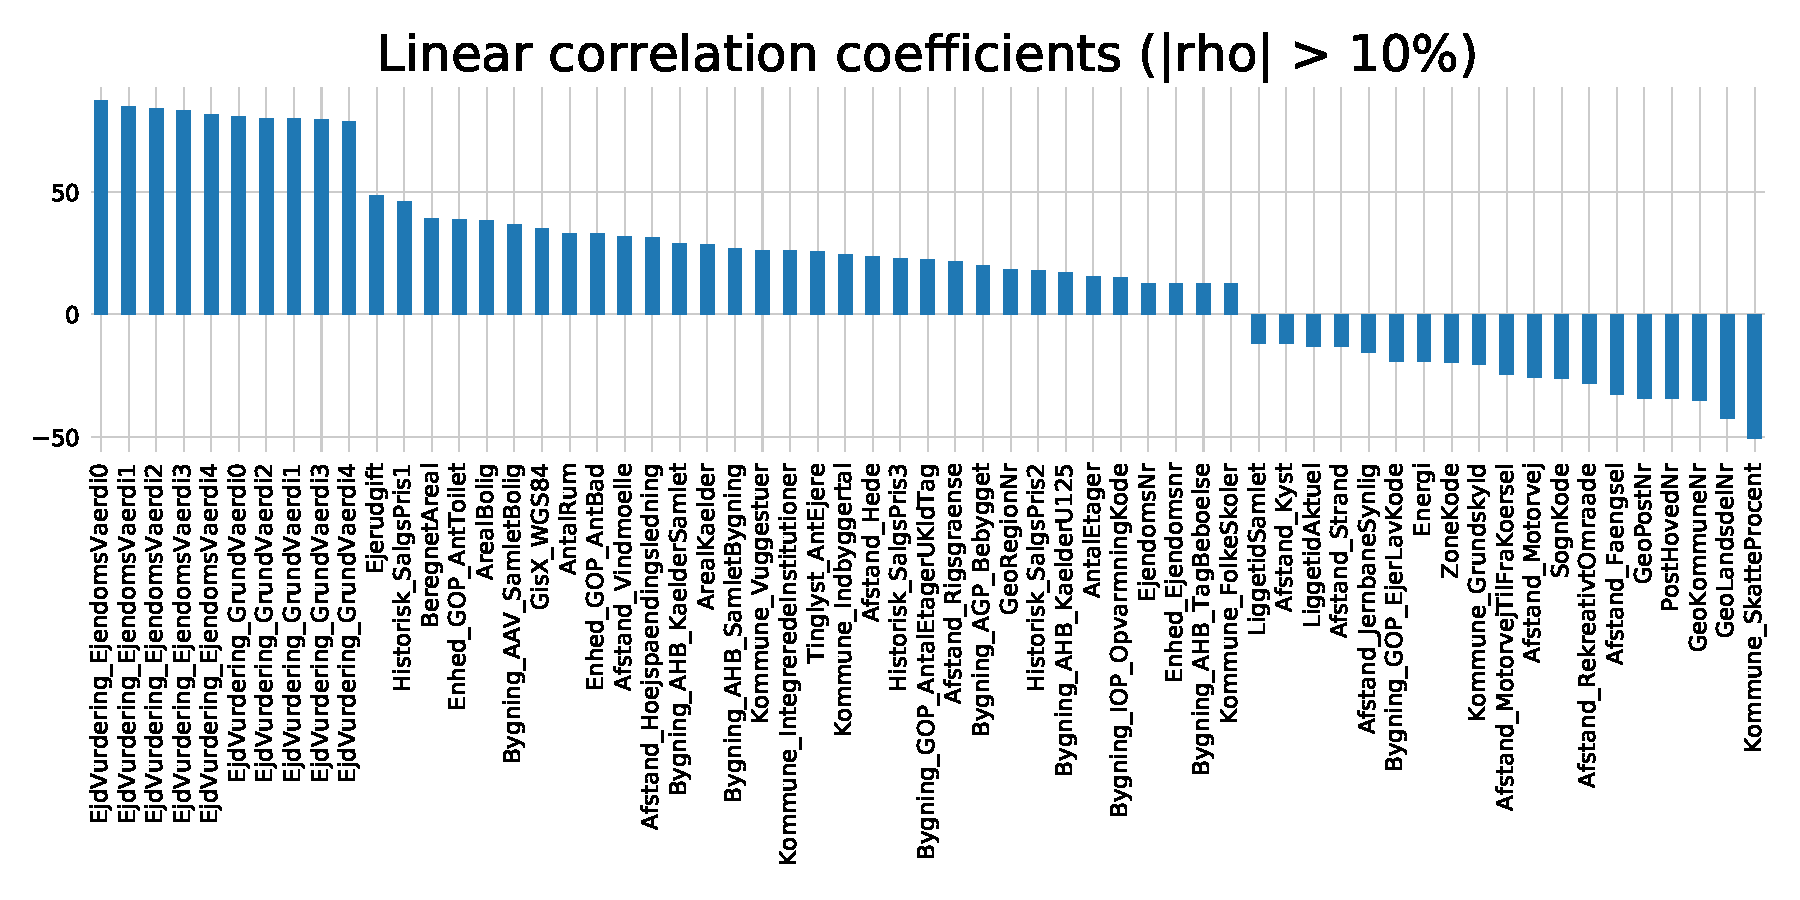
\includegraphics[width=0.99\textwidth, trim=0 10 0 40, clip]{figures/housing/lin_correlation.pdf}
  \caption[Linear Correlation Between Variables and Price]
          {Linear correlation $\rho$ between each variable and the sales price for variables where $\abs{\rho} > \SI{10}{\percent}$.}
  \label{fig:h:corr_lin}
\end{figure*}

The correlation $\rho$ used above is the linear correlation which only captures linear relationships between variables. All modern machine learning algorithms, however, are also able to capture higher-order correlations and thus a higher-order correlation measure is needed. The maximal information coefficient (MIC), which is a value between \num{0} and \num{1}, is such a nonlinear measure\sidenote{Note, that contrary to the linear correlation, MIC is always positive.}. It finds correlation based on the intuition that if two variables are correlated, it should be possible to split the data up into smaller grids where, if they are correlated, the grid that contain points should contain many points and the rest of the grids should be (relatively) empty \autocite{reshefDetectingNovelAssociations2011}. This is in comparison to two uncorrelated variables which would simply display noisy behavior and only have few grids with many points in. \citet{albanesePracticalToolMaximal2018a} extended on this idea and developed the computationally efficient algorithm called MICtools which computes the estimator $\mathrm{MIC}_e$ for MIC. An example of this nonlinear correlation is seen in Figure~\ref{fig:h:MIC_example_small}. Here the relationship between the normal linear correlation $\rho$ and $\mathrm{MIC}_e$ are shown for four synthetic datasets. Notice that $\mathrm{MIC}_e$ performs particularly well for the sine wave, and decent for the line and parabola, but only slightly captures the relationship for the exponential growth. The influence of noise on $\rho$ and $\mathrm{MIC}_e$ is shown in Figure~\ref{fig:h:MIC_example}. 

\begin{figure}
  \centerfloat
  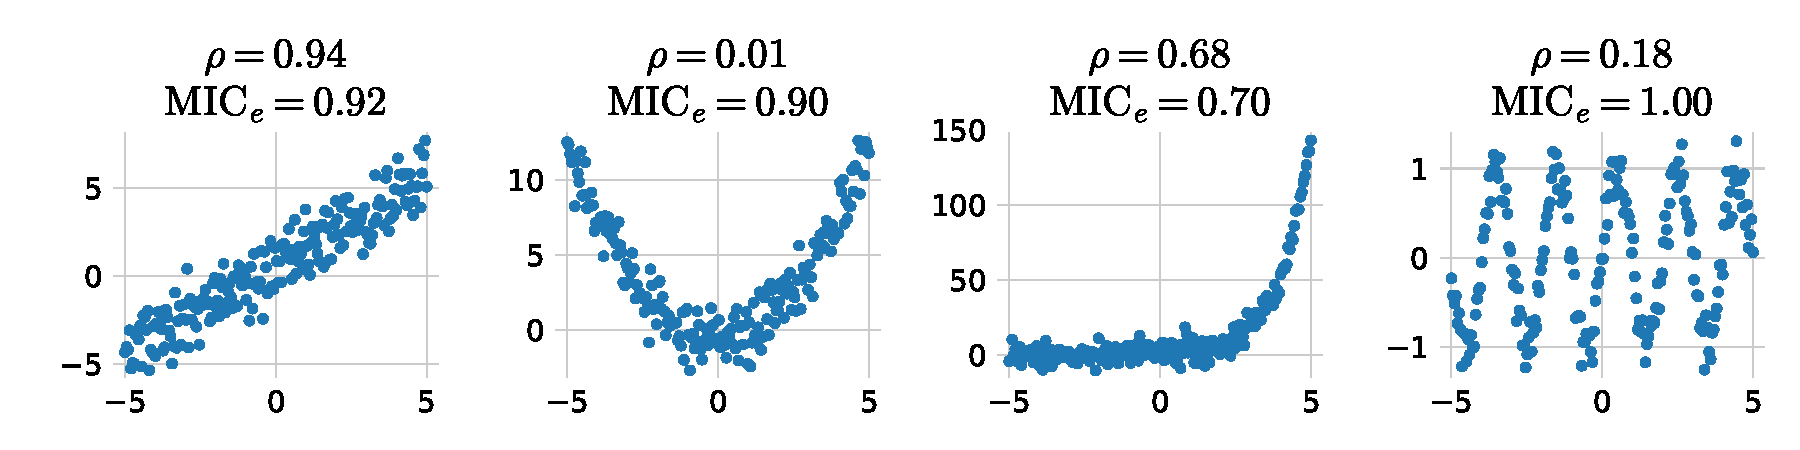
\includegraphics[width=0.99\textwidth, trim=10 10 10 10, clip]{figures/housing/MIC_test_small.pdf}
  \caption[Comparison of the Linear Correlation $\rho$ and the Nonlinear MIC]
          {Comparison of the linear correlation $\rho$ and the nonlinear MIC for a straight line, a parabola, an exponential, and a sine wave, all with noise added. See also Figure~\ref{fig:h:MIC_example}.}
  \label{fig:h:MIC_example_small}
\end{figure}

Using $\mathrm{MIC}_e$ as the correlation measure between the numerical variables and the sales prices, the variables with a $\mathrm{MIC}_e$-score higher than \SI{10}{\percent} are shown in Figure~\ref{fig:h:corr_MIC}. Again, the previous property evaluations are the most correlated features to the sales price followed by the parish code, \code{SogneKode}. In general the geographical variables score high here with also the post code and municipality number. 

\begin{figure*}
  \centerfloat
  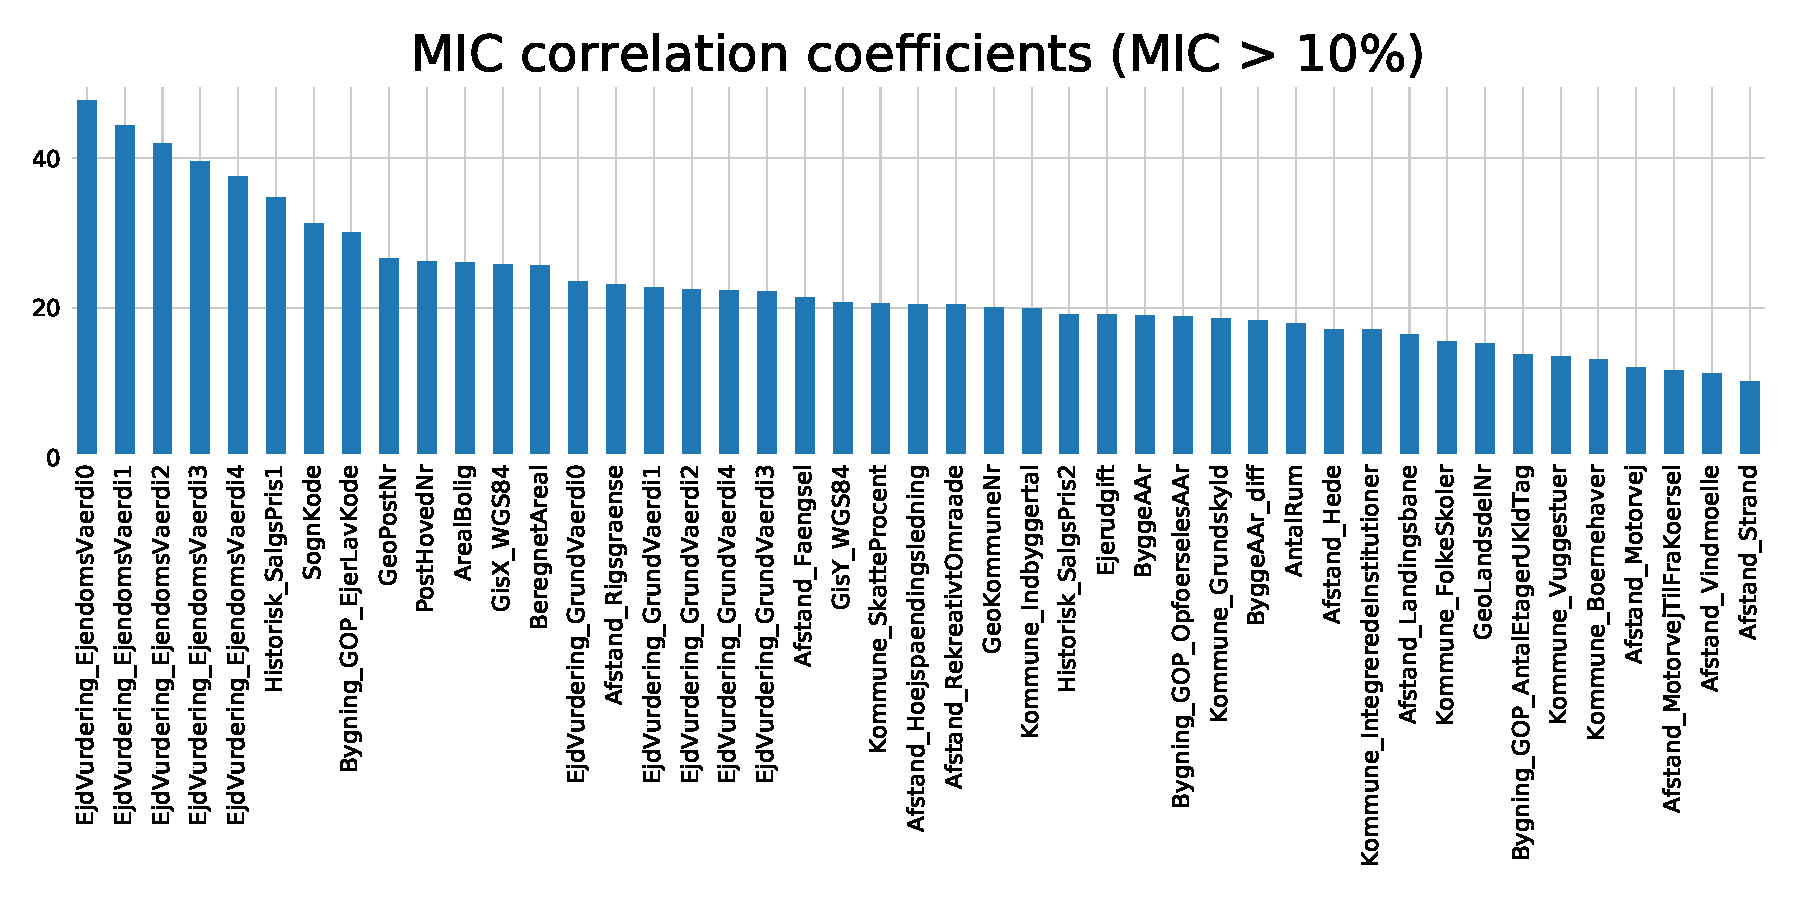
\includegraphics[width=0.99\textwidth, trim=0 10 0 40, clip]{figures/housing/MIC_plot.pdf}
  \caption[Nonlinear Correlation Between Variables and Price]
          {Nonlinear correlation between variables and price using Maximal Information Coefficient (MIC) for variables where $\text{MIC}>10\%$.}
  \label{fig:h:corr_MIC}
\end{figure*}

\subsection{Validity of Input Variables}

The fact that some of the variables contain considerable amounts of invalid values, NANs, requires this to be taken into account before any further analysis. The validity, defined as the percentage of valid observations, of every variable is shown in Figure~\ref{fig:h:nans}. Here the \num{168} variables are grouped together into \num{25} groups where each group share the same validity. An example of this is all of the \num{16} different distance-variables\sidenote{Distance to: prison, heath, high-voltage transmission line, industry, visible railroad, church, churchyard, coast, landing strip, motorway, access to motorway, recreational area, border, sports centre, beach, and windmill.}. We see that most of the variables have validities around more than 
\SI{85}{\percent}, however, a few of the variables, especially information about the building, \code{BygningsInfo}, have validities less than \SI{20}{\percent}. 

% \sidenote{Distance to: Fængsel, Hede, Højspaendingsledning, Industri, JernbaneSynlig, Kirke, Kirkegård, Kyst, Landingsbane, Motorvej, MotorvejTilFraKørsel, RekreativtOmråde, Rigsgrænse, Sportsanlæg, Strand, Vindmølle}

\begin{figure*}
  \centerfloat
  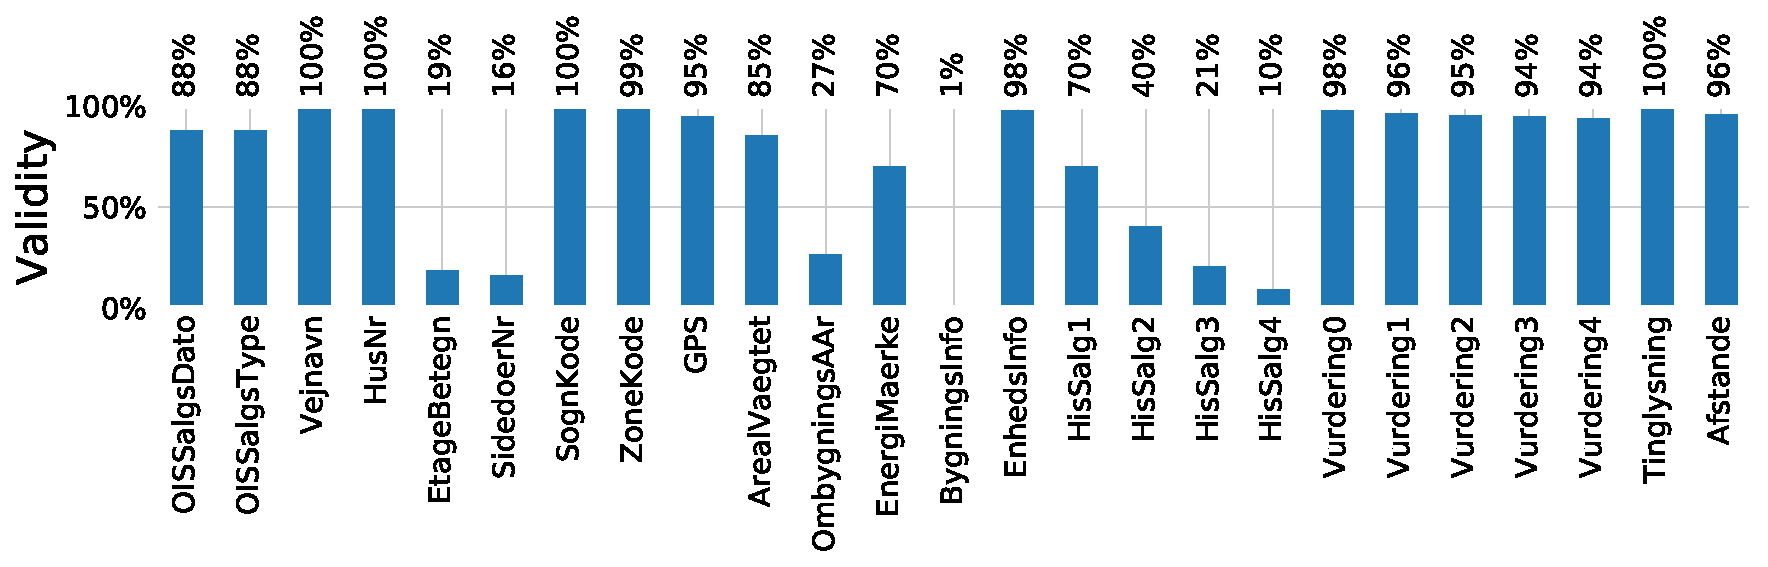
\includegraphics[width=\textwidth, trim=0 0 0 0, clip]{figures/housing/missing_bar.pdf}
  \caption[Validity of Input Features]
          {Percentage of valid counts for each variable grouped together in categories.}
  \label{fig:h:nans}
\end{figure*}

To see how closely related the different validity groups are, one can look at the dendrogram in Figure~\ref{fig:h:nans_dendrogram}. The dendrogram is based on a hierarchical clustering algorithm \citep{virtanenSciPyFundamentalAlgorithms2019} where the different groups are clustered according to the linear correlation of their validity. This diagram is supposed to be read in a top-down approach, where it can be seen that the name of the street, \code{Vejnavn}, and the number of the residence, \code{HusNr}, correlate a lot and are thus clustered very early. The year of the last time the residence was rebuilt or greatly modified, \code{OmbygningsAAr}, does not correlate strongly with any of the other variables and is thus the last variable to be clustered together. A heatmap of the validity inter-variable correlations is shown in Figure~\ref{fig:h:nans_heatmap}. 

\begin{figure}
  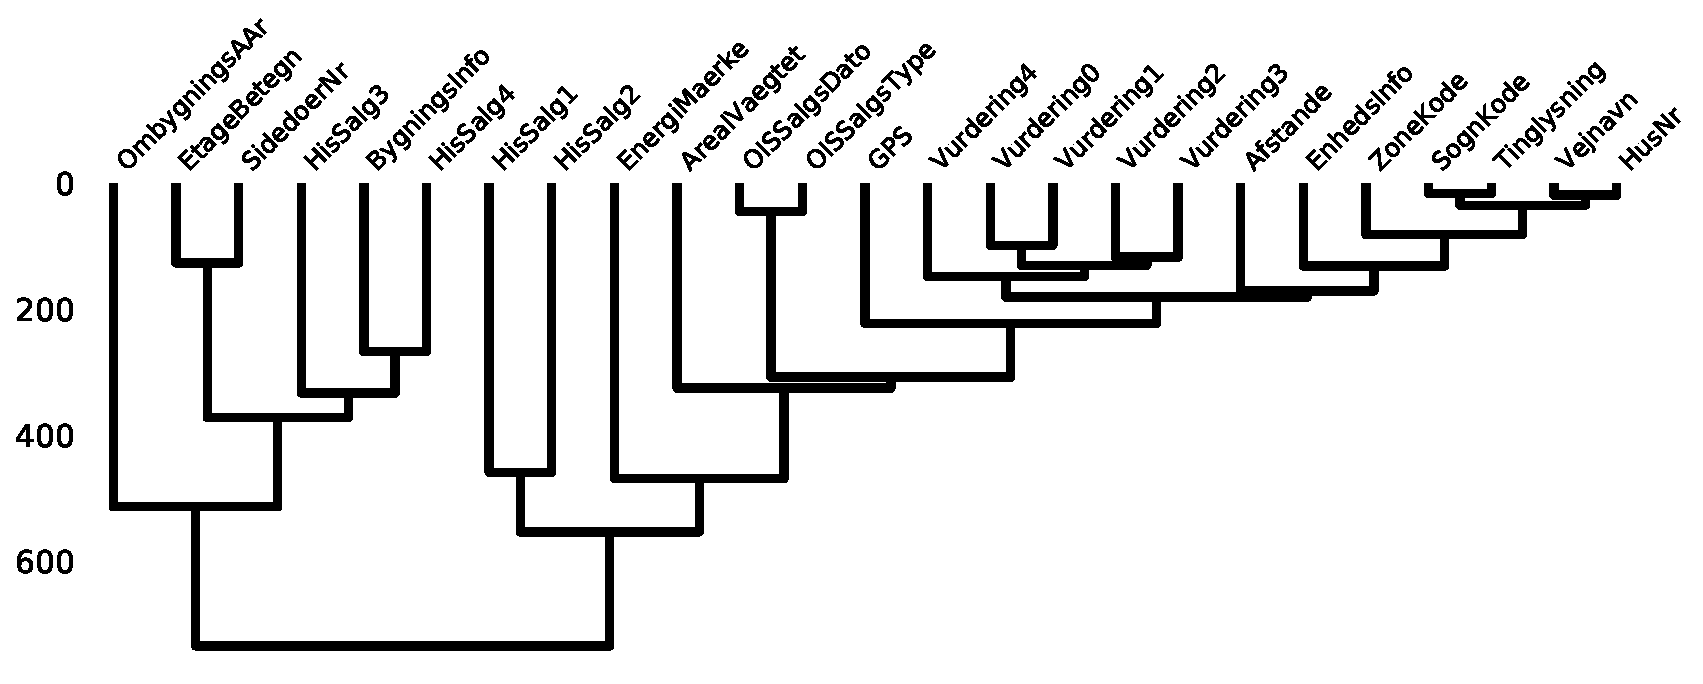
\includegraphics[width=0.98\textwidth, trim=35 10 0 10, clip]{figures/housing/missing_dendrogram.pdf}
  \caption[Validity Dendrogram]
          {Validity Dendrogram based on hierarchical clustering of the linear correlation of validity for the housing price variables clustered together.}
  \label{fig:h:nans_dendrogram}
\end{figure}


\subsection{Selection Criteria}
Given the 1D input variable distributions and their validity, we apply some very basic selection criteria before any further analysis. These selection criteria are shown in Table \ref{tab:h:initial_cuts}. 

\begin{table}[h]
  \begin{tabular}{@{}llcr@{}}
  % \toprule
               & Description                                          & Remaining & Removed \\ 
  \midrule
  Area         & \SI{20}{\meter\squared} $\leq$ Area $\leq$ \SI{500}{\meter\squared} & \num{689140}              & \num{23666}     \\
  Price        & \SI{0.1}{\Mkr} $\leq$ Price $\leq$ \SI{100}{\Mkr}                   & \num{687546}              & \num[group-minimum-digits=3]{1594}      \\
  Type         & Has sales type \num{1}                                              & \num{605415}              & \num{82131}     \\
  GPS          & Has valid GPS coordinates                                           & \num{578860}              & \num{26555}     \\
  Private      & Only non-business sales                                             & \num{549140}              & \num{29720}     \\
  Time         & Sold in \num{2009} or later                                         & \num{520548}              & \num{28592}     \\
  \bottomrule
  \end{tabular}
  \caption[Basic Selection Criteria]{Overview of the basic selection criteria which define the minimum information needed to predict the price of a sale.}
  \label{tab:h:initial_cuts}
\end{table}

The sales type, \code{OISSalgsType}, is an OIS\sidenote{OIS is short for \q{Den Offentlige Informationsserver}, the Danish public information server, and it collects information about Danish residences \autocite{oisWwwOISDk}.} code which describes what type of sale it is: when it is \num{1} it is considered a normal sale, compared to e.g. forced sales. These cuts are seen as the minimum requirements for what constitutes a curated dataset with no obvious outliers. The reason why the time requirement is applied is to reduce the effect of the financial crisis to creep into the model. 


\section{Feature Augmentation}
\label{sec:h:feature_augmentation}

The analysis have dealt with different types of residences all together until now. The rest of the analysis will be applied on single-family houses and owner-occupied apartments independently from this point on. 

\begin{margintable}[3cm]
  % \begin{tabular}{llr}
  \begin{tabular*}{\textwidth}{l @{\extracolsep{\fill}} lr}
  % \toprule
  String & Explanation  & Code \\ \midrule
  NAN    & No side door & \num{0}    \\
  TH, TV & Right, left  & \num{11}   \\
  MF     & Center       & \num{12}   \\
  --     & The rest     & \num{15} 
  \end{tabular*}
  \vspace{1mm}
  \caption[Side Door Mapping.]{Side door mapping. If the side door string contains e.g. \q{TH} this gets the code \num{11}.}
  \label{tab:h:sidedoor_code}
  \vspace{3mm}
\end{margintable}

First, invalid counts are dropped such that variables which contain more than \SI{10}{\percent} NANs are dropped, and duplicate rows are also removed. Then some manual features are added based on existing features. The day of the month, the month, and the year are extracted from the sales date. The sales date is converted to the numbers of days since January \nth{1}, \num{2009}. From the number of the house, \code{HusNr}, the value is extracted along with a boolean flag indicating whether or not it includes a letter (eg. \q{27B}). The number of the side door, \code{SidedoerNr}, is formatted according to Table~\ref{tab:h:sidedoor_code} and the road name according to  Table~\ref{tab:h:road_code}. The age of the house is added\sidenote[][-1cm]{In addition to only having the year the house was was built.} and the amount of time (in years) since last major modification. The energy rating label, \code{EnergiMaerke}, is also converted from strings to values according to Table~\ref{tab:h:energy_code}.

\begin{margintable}
  \begin{tabular*}{\textwidth}{l @{\extracolsep{\fill}} lr}
  Contains   & Explanation  & Code \\ \midrule
  Vej        & Road       & \num{0}    \\
  Gade       & Street     & \num{1}    \\
  Alle, Allé & Avenue     & \num{2}    \\
  Boulevard  & Boulevard  & \num{3}    \\
  --         & The rest   & \num{-1}  
  \end{tabular*}
  \vspace{1mm}
  \caption[Street Mapping]{Street mapping. If the street name contains e.g. \q{Vej} this gets the code \num{0}.}
  \label{tab:h:road_code}
  \vspace{3mm}
\end{margintable}

Finally, some of the variables in the dataset are not suitable for machine learning (or are simply transformations of other variables) and are thus dropped. These are variables such as the ID, when the house was deleted at Boligsiden, or the cash price.

\subsection{Time-Dependent Price Index}

In addition to the manual data augmentation, a time-dependent price index is also added. We make use of the open source package called Prophet made by \citet{taylorForecastingScale} at Facebook. It is based on a decomposable time series model \autocite{harveyEstimationProceduresStructural1990} with two\sidenote{In their paper, \citet{taylorForecastingScale} include a holiday component in their analysis as well which is not included in this project.} components; the trend $g(t)$ and the seasonality $s(t)$:
\begin{equation}
  y_\mathrm{Prophet}(t) = g(t) + s(t) + \epsilon_t,
\end{equation}
where $\epsilon_t$ is a normally distributed error term. \citet{taylorForecastingScale} fit this equation with a generalized additive model (GAM) \autocite{hastieGeneralizedAdditiveModels1987} which they argue has several practical advantages compared to ARIMA\sidenote{AutoRegressive Integrated Moving Average.} models which are commonly used in economics \autocite{nla.cat-vn1067782}. 

We fit the Prophet model on the weekly median price pr. square meter (PPSM) up until (and including) \num{2017}. The results of the prophet model fitted on (owner-occupied) apartments are seen in Figure~\ref{fig:h:prophet_forecast} and Figure~\ref{fig:h:prophet_trends}. In Figure~\ref{fig:h:prophet_forecast} the weekly median price pr. square meter for apartments are shown as black dots with the fitted Prophet model shown in blue. The $1\sigma$ uncertainty intervals are shown as the transparent blue band. The Prophet model not only allows predicting previous and future PPSMs, it also return the uncertainty of this prediction. The future predictions for the PPSM are the values after 2018. The trend and seasonality of the model are shown in Figure~\ref{fig:h:prophet_trends} where the top plot is the overall trend $g(t)$ and the bottom plot is the seasonality $s(t)$. Whereas the trend just continues to rise, the seasonality shows that residences are generally sold for a higher price in the Summer months compared to the Winter months. 
The Prophet model plots for one-family houses are shown in Figure~\ref{fig:h:prophet_forecast_villa} and \ref{fig:h:prophet_trends_villa}. 

\begin{figure}
  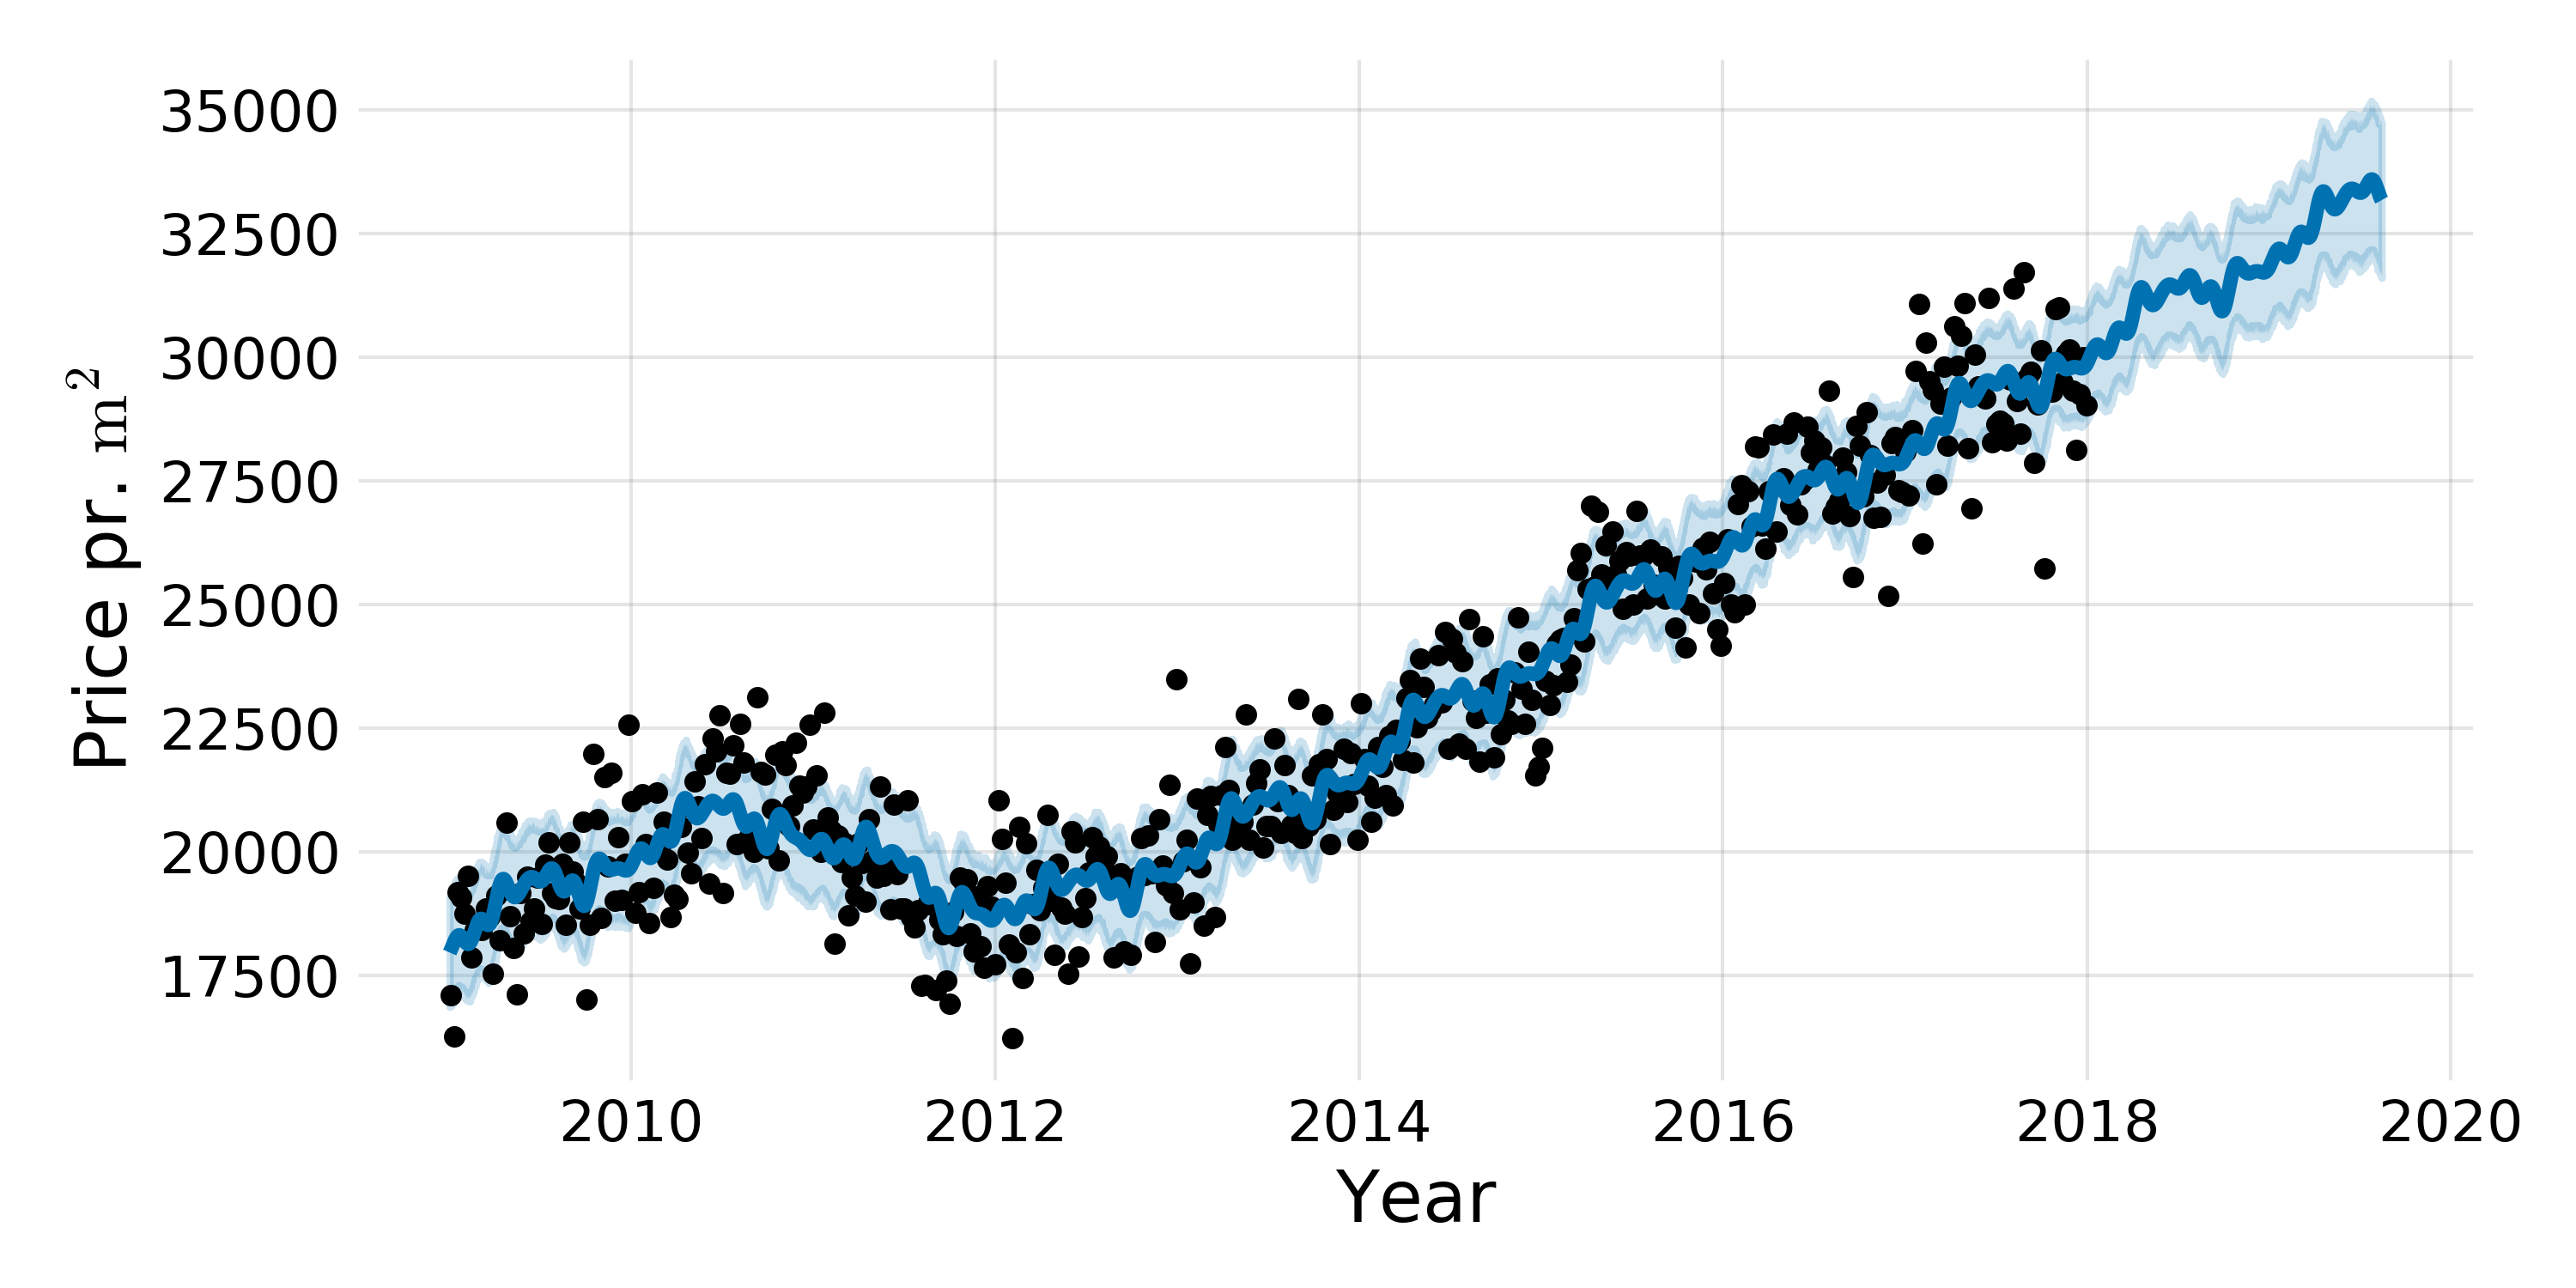
\includegraphics[draft=false, width=0.9\textwidth, trim=15 15 15 15, clip]{figures/housing/Ejerlejlighed_v18_cut_all_Ncols_all_prophet_forecast.png}
  \caption[Prophet Forecast for Apartments]
          {The predictions of the Facebook Prophet model trained on square meter prices for owner-occupied apartments sold before January 1st, 2018. The data is down-sampled to weekly bins where the median of each week is used as in input to the Prophet model, shown seen as black dots in the figure. The \textcolor{blue}{model's forecasts} for 2018 and 2019 are shown in blue with a light blue error band showing the $1\sigma$ confidence interval.
          }
  \label{fig:h:prophet_forecast}
\end{figure}

\begin{figure}
  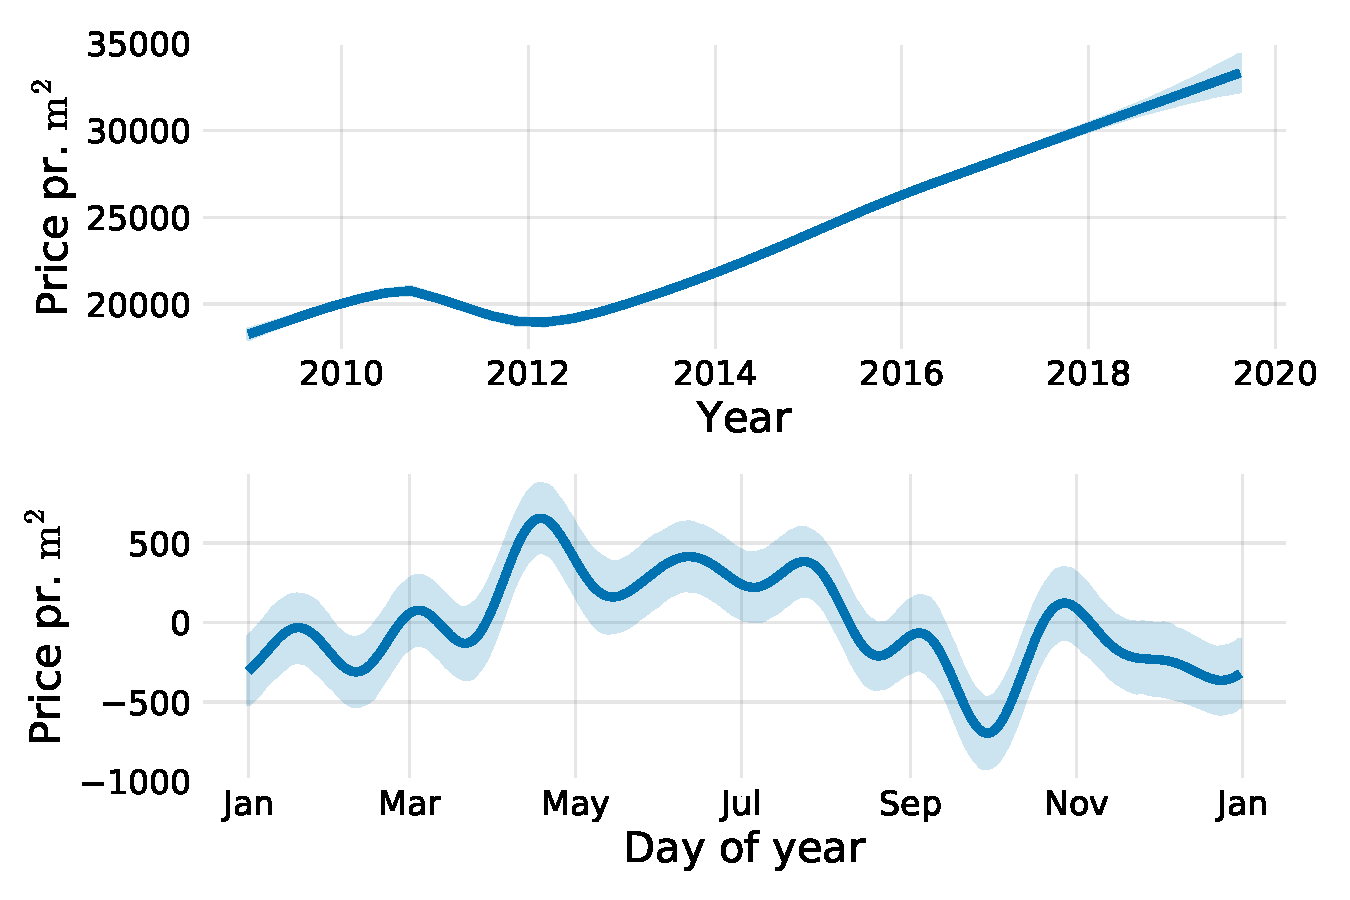
\includegraphics[draft=false, width=0.9\textwidth, trim=15 15 15 15, clip]{figures/housing/Ejerlejlighed_v18_cut_all_Ncols_all_prophet_trends.pdf}
  \caption[Prophet Trends]
          {The trends of the Facebook Prophet model trained on square meter prices for owner-occupied apartments sold before January 1st, 2018. In the top plot is the overall trend as a function of year and in the bottom plot is the yearly variation as a function of day of year. It can be seen that the square meter price is higher during the Summer months compared to the Winter months, however, compared to the overall trend this effect is minor ($<10\%$). 
          }
  \label{fig:h:prophet_trends}
\end{figure}

Using the Prophet model, we define the price index (PI) to be the Prophet-predicted PPSM, $y_\mathrm{Prophet}$, for each residence normalized by the mean to give values around \num{1}:
\begin{equation}
  % \mathrm{PI}(t) = \frac{y_\mathrm{Prophet}(t)}{\mathrm{mean}(y_\mathrm{Prophet}(t))}.
  \mathrm{PI}(t) = \frac{y_\mathrm{Prophet}(t)}{\langle y_\mathrm{Prophet}(t) \rangle},
\end{equation}
where $\langle \boldsymbol{\cdot} \rangle$ refers to the average. The price index thus works as a measure of the national price for houses or apartments at a given time and is added as a variable to the dataset. 

% \begin{figure}
%   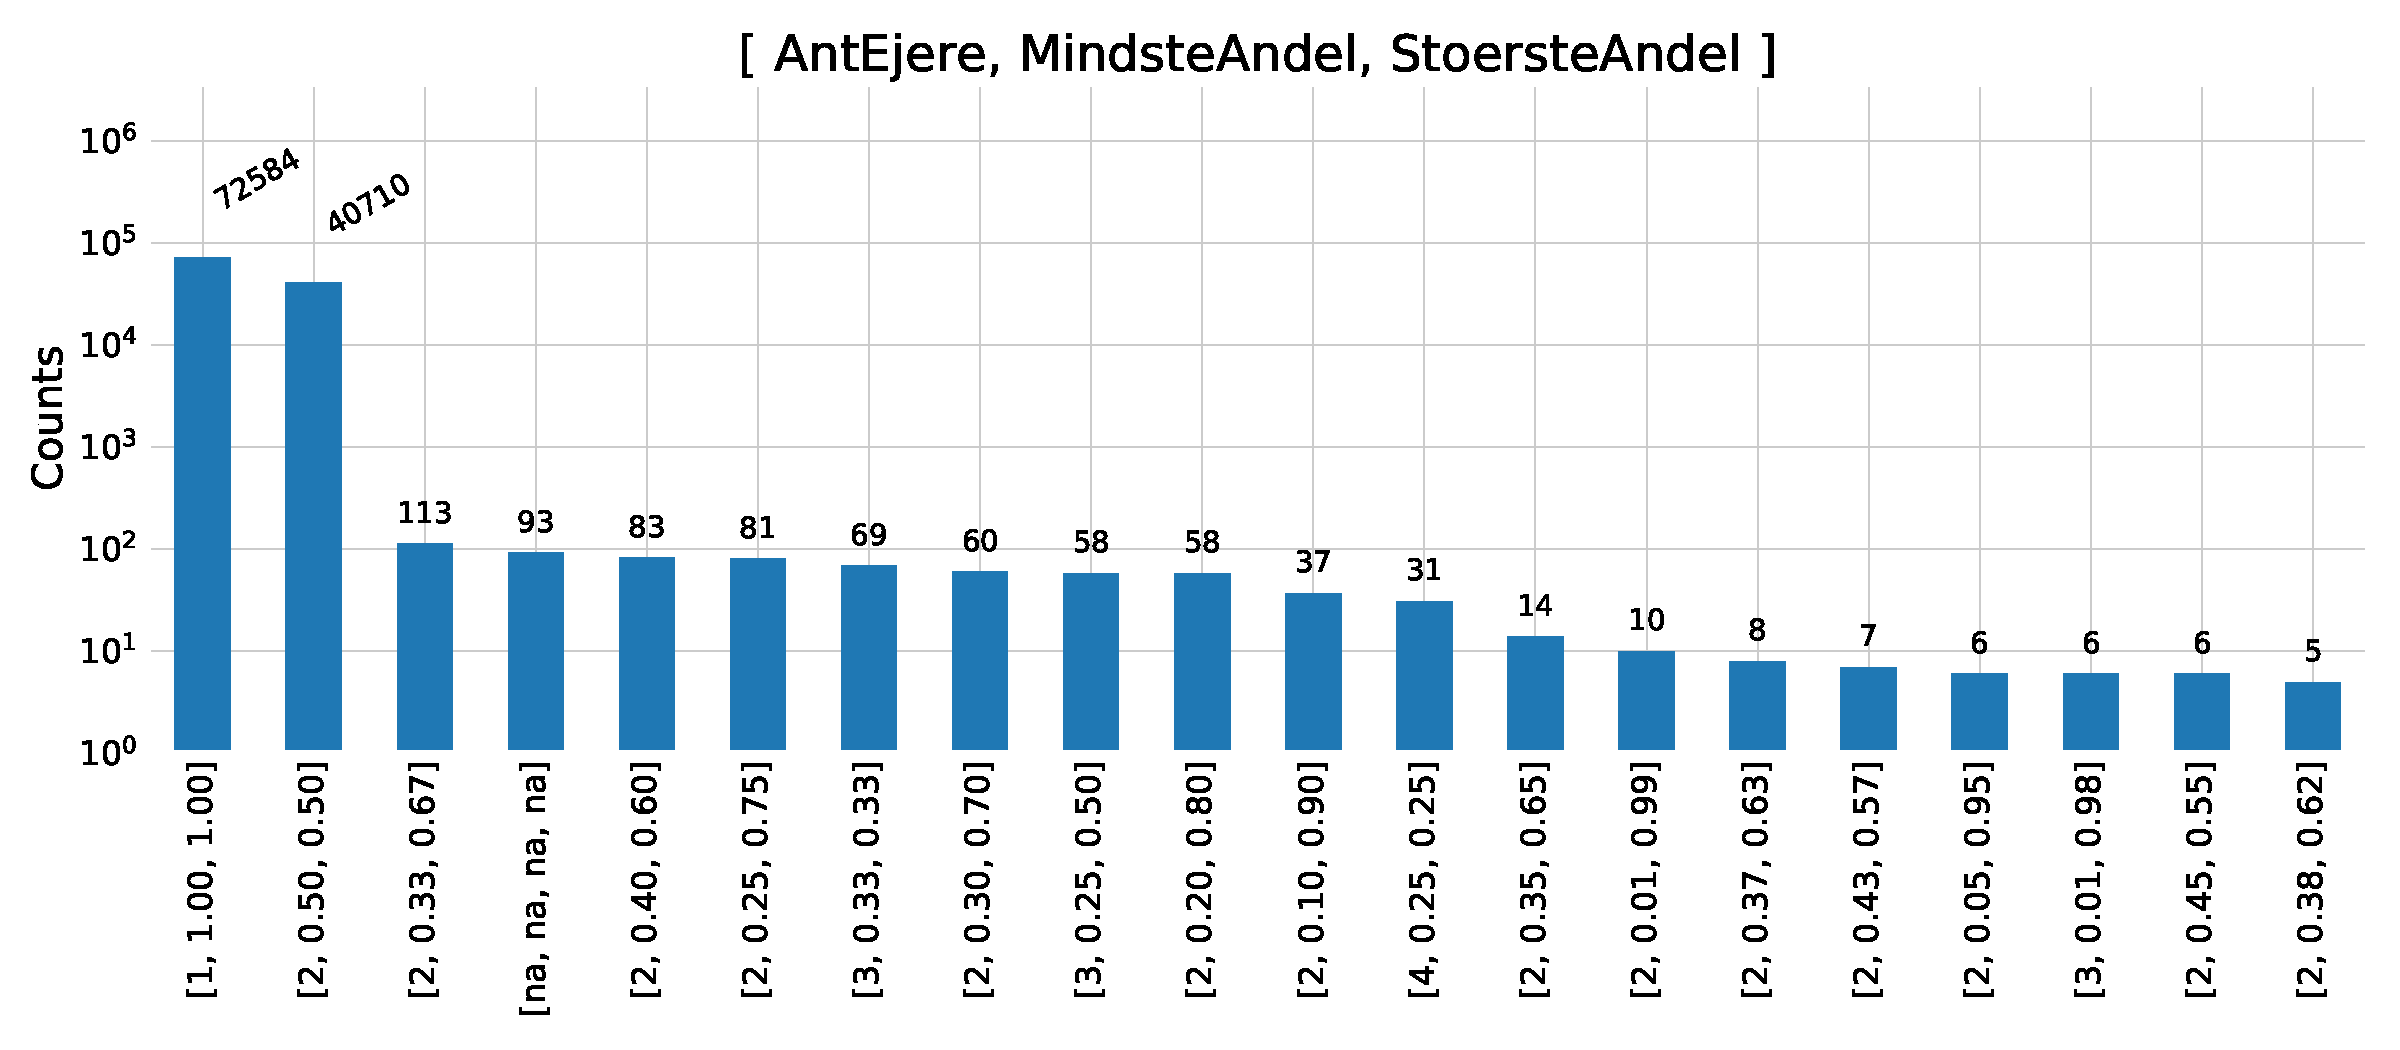
\includegraphics[width=0.9\textwidth]{figures/housing/tinglysning_fig.pdf}
%   \caption[Registration of property]
%           {Overview of registration of property as a function of amount of owners (\code{AntEjere}), lowest share (\code{MindsteAndel}) and biggest share (\code{StoersteAndel}) written as \code{[AntEjere, MindsteAndel, StoersteAndel]}.
%           }
%   \label{fig:h:tinglysning}
% \end{figure}

\section{Evaluation Function}
\label{sec:h:evaluation_function}

The choice of evaluation function $f_\mathrm{eval}$ is an important decision. The evaluation function will be based on the relative prediction $z_i$: 
\begin{equation}
  z_i = \frac{\hat{y}_i-y_i}{y_i},
\end{equation}
where $y_i$ is the true price and $\hat{y}_i$ the predicted one. The relative prediction is defined such that it is positive when $\hat{y}_i>y_i$. Due to the outlier selection criteria applied earlier, the denominator is made sure to always be positive (and never \num{0}), and $\vec{z}$ is expected to approximately follow a normal distribution\sidenote{Where $\vec{z}$ is the vector of all relative predictions $\vec{z} \in \mathbb{R}^N$.}. Initially the mean of $\vec{z}$ was considered as the choice of evaluation function $f_\mathrm{eval}\stackrel{?}{=} \mathrm{mean}(\vec{z})$ though this only ensures a minimum of bias, not necessarily a low spread. This lead the discussion on to look at the standard deviation of $z$ as $f_\mathrm{eval}\stackrel{?}{=} \mathrm{std}(\vec{z})$. The mean and the standard deviation, however, are not very robust estimators since they are heavily influenced by outliers. The mean (and thus also the standard deviation) has an \emph{asymptotic breakdown point} at \SI{0}{\percent}, where the breakdown point is defined as the smallest fraction\sidenote{Where the \q{asymptotic} in \q{asymptotic breakdown point} refers to when the number of samples goes to infinity.} of bad observations that can cause an estimator to become arbitrarily small or large: a single outlier with an arbitrarily large value may cause the mean to diverge to that large value \autocite{huber2011robust}. In comparison, the median has an asymptotic breakdown point of \SI{50}{\percent} and is thus a more robust estimator of centrality. A robust measure of the variability or dispersion of a sample $\vec{x}$ (compared to e.g. the standard deviation $\sigma$) is the median absolute deviation (MAD) written as:
\marginnote{Here $\abs{\vec{x}}$ is the absolute value of $x_i$ applied element-wise and not the norm of the vector $\vec{x}$.}
\begin{equation}
  \mathrm{MAD}(\vec{x}) = c \cdot \mathrm{median} \left( \abs{\vec{x} - \mathrm{median}(\vec{x})} \right), \quad c = \frac{1}{\Phi^{-1}(\frac{3}{4})},
  \label{eq:h:MAD}
\end{equation}
where $c$ is a normalization constant to make MAD a consistent estimator of the standard deviation $\sigma$ assuming normally distributed data and $\Phi^{-1}$ is the percent point function\sidenote{Inverse of the cumulative distribution function.} \autocite{leysDetectingOutliersNot2013}.
The MAD is thus the median of the absolute differences between the data and the median of the data. We are, however, not just interested in having the distribution of $\vec{z}$ as narrow as possible, we also want it centered around \num{0}. We thus continue with the following evaluation function:
\begin{equation}
  \begin{split}
    \mathrm{MAD}_0(\vec{x})  &\equiv c \cdot  \mathrm{median} \left( \abs{\vec{x} - 0} \right) = c \cdot \mathrm{median} \left( \abs{\vec{x}} \right) \\
    f_\mathrm{eval}(\vec{z}) &\equiv \mathrm{MAD}_0(\vec{z}) = c \cdot  \mathrm{median} \left( \abs{\vec{z}} \right).
  \end{split}
\end{equation}
To get an intuition about the size of a \q{good} value of $\mathrm{MAD}_0$, one could calculate it comparing the asking price with the actual sales price. Doing so, one finds: $f_\mathrm{eval}(\vec{z}_\mathrm{OFH}) = \SI{11.35}{\percent}$ for houses and $f_\mathrm{eval}(\vec{z}_\mathrm{OOA}) = \SI{5.72}{\percent}$ for apartments. In some cases $f_\mathrm{eval}$ will still be referred to as MAD and it will be mentioned explicably if the form in equation \eqref{eq:h:MAD} is meant. 

\marginnote[-4cm]{The robust estimator MAD is derived assuming symmetric distributions. Robust measures of the variability of non-symmetric samples have also been developed, see \citet{rousseeuwAlternativesMedianAbsolute1993} for more details.}


\section{Initial Hyperparameter Optimization}
\label{sec:h:initial_hyperparameter_optimization}

With the initial cleaning and feature adding done, the shapes of the ML-ready datasets are: (\num{291317}, \num{144}) for houses (OFHs) and (\num{114166}, \num{144}) for apartments (OOA), both sharing the same variables. All of the variables which are used from this point on are shown in Table~\ref{tab:h:all_variables}. 
The data are split into training and test sets such that training is defined as every sale from before \num{2018}, the test set is every sale from \num{2018}, and, since more data came after the project started, \num{2019} is a small extra test set. 

\begin{margintable}[-8.5cm]
  \begin{tabular}{lrr}
              & Houses       & Apartments   \\ \midrule
   Train      & \num{240070} & \num{93115}  \\   
   Test       & \num{34628}  & \num{14183}  \\   
   \num{2019} & \num{16619}  & \num{6868} 
  \end{tabular}
  \vspace{1.5mm}
  \caption[Number of Observations in the Housing Dataset]{\label{tab:h:train_test_split}Number of observations for houses and apartments in the training, test, and \num{2019} set.}
  \vspace{3mm}
\end{margintable}

\begin{margintable}[-3cm]
  \begin{tabular}{lrr}
% \begin{table}
  % \begin{tabular}{lll}
   Tight      & Houses        & Apartments  \\ \midrule
   Train      & \num{143179}  & \num{57795} \\   
   Test       & \num{20338}   & \num{8376}  \\   
   \num{2019} & \num{9683}    & \num{4030} 
  \end{tabular}
  \vspace{1.5mm}
  \caption[Number of Observations in the Housing Dataset for the Tight Selection]{\label{tab:h:train_test_split_tight}Number of observations for houses and apartments in the training, test, and \num{2019} set for the tight selection.}
  \vspace{3mm}
\end{margintable}

The number of observations for the different sets are shown in Table~\ref{tab:h:train_test_split}. Since the dataset has been shown to be quite noisy with a lot of invalid counts a \emph{tight} selection of the data is also applied. The tight selection is defined as residences which are within the \SI{1}{\percent} to \SI{99}{\percent} quantiles of all\sidenote[][-1.5cm]{Except the variables that contains the words: \q{aar} (year), \q{dato} (date), and  \q{prophet}.} numeric variables with more than 3 unique values. The number of observations for the different tight sets are shown in Table~\ref{tab:h:train_test_split_tight}. 

A small study into the effect of some various hyperparameters was performed before any further fitting. This study investigated the effect of the old sales by assigning them a lower weight depending on time. It was investigated whether or not the model would perform better if samples got the time-dependent weight $w(t)$ given by:

\begin{marginfigure}[-0.5cm]
  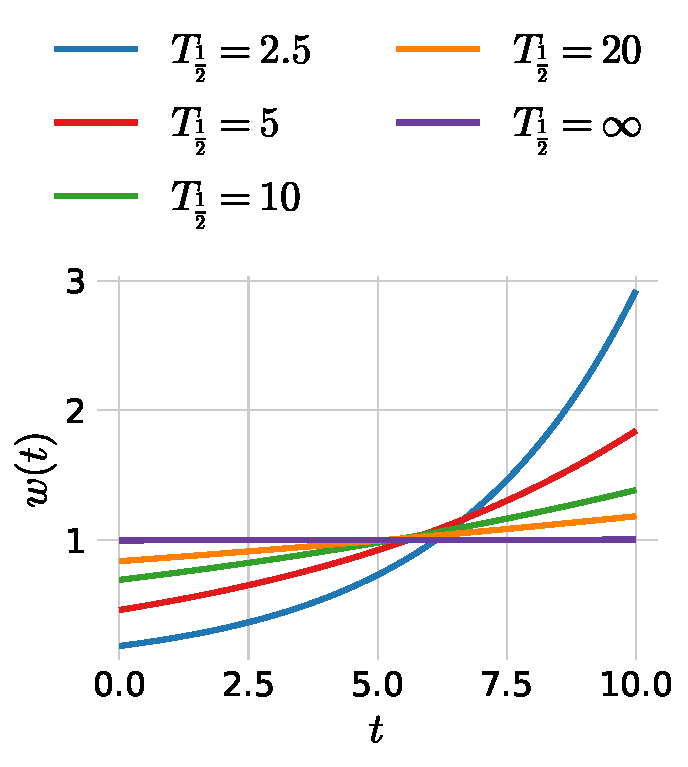
\includegraphics[width=0.99\textwidth]{figures/housing/Villa_v18_cut_all_Ncols_all_half_life_weights.pdf}
  \caption[Sample Weight as a Function of Time for Different Half-Lives.]
    {The sample weight $w(t)$ as a function of time $t$ where the time is in years after January \nth{1}, 2009, Here seen plotted for different values of the half-life $T_{\frac{1}{2}}$.}
  \label{fig:h:half-life}
\end{marginfigure}

\begin{equation}
  \begin{split}
    w'(t) &= e^{ k \cdot t}, \quad k = \frac{\log 2}{T_{\frac{1}{2}}} \, ,\\
    w(t) &= \frac{w'(t)}{\langle w'(t) \rangle} \, ,
  \end{split}
  \label{eg:h:sample_weight}
\end{equation}
% TODO: add parts about what weights are.

\noindent where $T_{\frac{1}{2}}$ is the half-life. This is illustrated in Figure~\ref{fig:h:half-life} for the different values of $T_{\frac{1}{2}}$ used in the study.  In addition to the weight, it was also investigated whether or not a $\log_{10}$-transformation of the price would increase performance. Finally the choice of loss function was also added to the study for the five different loss functions defined in \autoref{sec:ml:loss_function}. A grid search\sidenote[][-2cm]{Grid search was acceptable since the parameter space is small and two of the three dimensions are non-numerical.} was performed for:
\begin{equation}
  \begin{split}
    T_{\frac{1}{2}} &\in \{2.5,\, 5,\, 10,\, 20,\, \infty \}~\mathrm{ years} \\
    \log_{10} &\in \{\mathrm{True},\, \mathrm{False} \} \\
    \ell &\in \{ \ell_\mathrm{Cauchy},\, \ell_\mathrm{Fair},\, \ell_\mathrm{LogCosh},\, \ell_\mathrm{SE},\, \ell_\mathrm{Welsch}\}.
  \end{split}
\end{equation}

\begin{margintable}[-1cm]
  \begin{tabular}{@{}ccrc@{}}
    %\toprule
    Half-life & $\log_{10}$ & $N_\mathrm{trees}$ & $f_\mathrm{eval}$ \\
    \midrule
    \num{2.5} & True & \num{293} & \num{0.1598} \\
    \num{2.5} & False & \num{814} & \num{0.1466} \\
    \num{5} & True & \num{304} & \num{0.1610} \\
    \num{5} & False & \num{923} & \num{0.1468} \\
    \num{10} & True & \num{266} & \num{0.1610} \\
    $\mathbf{10}$ & \textbf{False} & $\mathbf{770}$ & $\mathbf{0.1450}$ \\
    \num{20} & True & \num{288} & \num{0.1613} \\
    \num{20} & False & \num{967} & \num{0.1467} \\
    $\infty$ & True & \num{340} & \num{0.1601} \\
    $\infty$ & False & \num{807} & \num{0.1480} \\
    %\bottomrule
  \end{tabular}
  \vspace{1.5mm}
  \caption[Results from the Initial Hyperparameter Optimization for Apartments]{\label{tab:h:HPO_initial_Cauchy-ejerlejlighed}Results of the initial hyperparameter optimization for apartments for the best loss function $\ell_\mathrm{Cauchy}$. The best hyperparameter is shown in bold.}
\end{margintable}


\begin{margintable}[0.5cm]
  \begin{tabular}{@{}ccrc@{}}
    %\toprule
    Half-life & $\log_{10}$ & $N_\mathrm{trees}$ & $f_\mathrm{eval}$ \\
    \midrule
    \num{2.5} & True & \num{434} & \num{0.1991} \\
    \num{2.5} & False & \num{1007} & \num{0.1872} \\
    \num{5} & True & \num{350} & \num{0.1999} \\
    \num{5} & False & \num{1130} & \num{0.1858} \\
    \num{10} & True & \num{436} & \num{0.1992} \\
    \num{10} & False & \num{1183} & \num{0.1850} \\
    \num{20} & True & \num{397} & \num{0.2003} \\
    $\mathbf{20}$ & \textbf{False} & $\mathbf{1514}$ & $\mathbf{0.1833}$ \\
    $\infty$ & True & \num{449} & \num{0.1992} \\
    $\infty$ & False & \num{1351} & \num{0.1844} \\
    %\bottomrule
  \end{tabular}
  \vspace{1.5mm}
  \caption[Results from the Initial Hyperparameter Optimization for Houses]{\label{tab:h:HPO_initial_Cauchy-villa}Results of the initial hyperparameter optimization for houses for the best loss function $\ell_\mathrm{Cauchy}$. The best hyperparameter is shown in bold.}
\end{margintable}


The grid search is performed for two boosted decision tree models based on XGBoost \autocite{chenXGBoostScalableTree2016} (XGB), one for apartments and one for houses. They were each training with \num{5}-fold cross validation and early stopping was applied with a patience of \num{100}. 

For apartments, the loss function with the lowest $f_\mathrm{eval}$ was the Cauchy loss with $T_{\frac{1}{2}}=10$ years and no $\log_{10}$-transformation. This model terminated by early stopping after \num{770} trees, see Table~\ref{tab:h:HPO_initial_Cauchy-ejerlejlighed}. 
For houses the loss function with the lowest $f_\mathrm{eval}$ was (also) the Cauchy loss with $T_{\frac{1}{2}}=20$ years and (also) no $\log_{10}$-transformation. This model terminated by early stopping after \num{1514} trees, see Table~\ref{tab:h:HPO_initial_Cauchy-villa}. 
It is interesting to note, that the best results for both houses and apartments share the same loss function and no $\log_{10}$-transformation. 

The $\log_{10}$-transformation was included as some machine learning methods assume that the dependent variable, $y$, is normally distributed. Initially, it also showed better results than no transformation, however, this turned out to be a numerical consequence which was alleviated by dividing all prices with a million, such that $y$ had units of \si{\Mkr} instead of \si{\kr} All of the results for the apartments are shown in Tables~\ref{tab:h:HPO_initial_Rmse-ejerlejlighed-appendix} to \ref{tab:h:HPO_initial_Fair-ejerlejlighed-appendix} along with all of the results for the houses in Tables~\ref{tab:h:HPO_initial_Rmse-villa-appendix} to \ref{tab:h:HPO_initial_Fair-villa-appendix}. 

\begin{figure}[h!]
  \centerfloat
  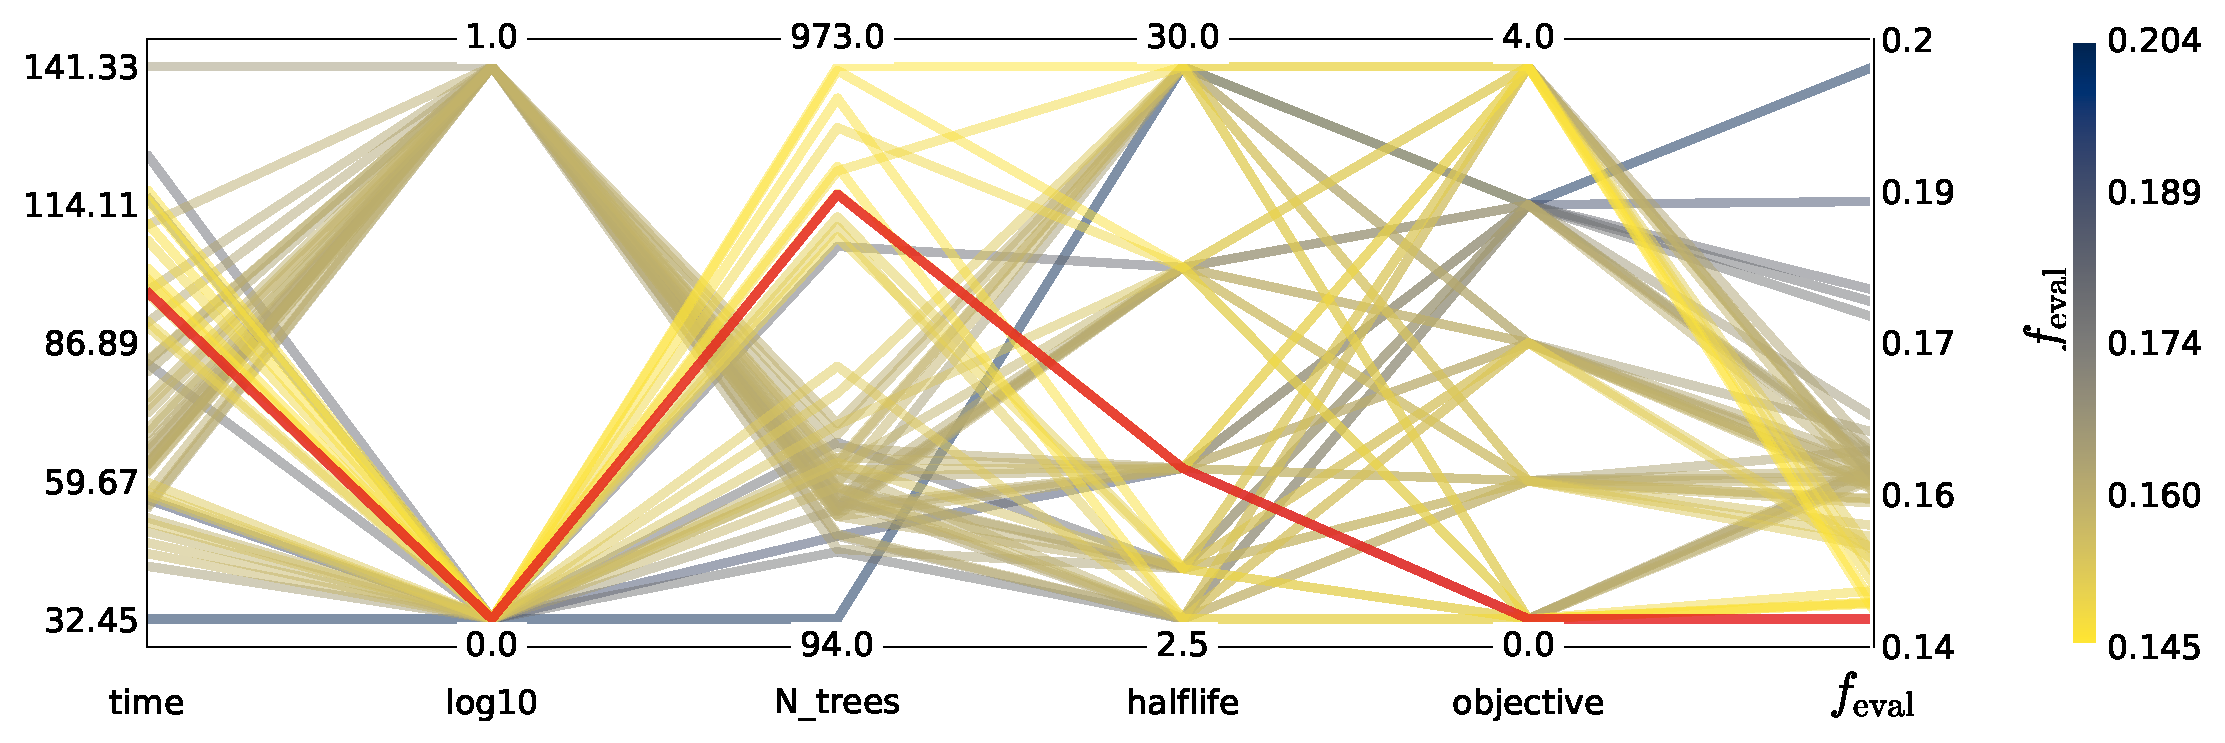
\includegraphics[width=0.99\textwidth, trim=0 0 0 0, clip]{figures/housing/Ejerlejlighed_v19_cut_all_Ncols_all_CV_viz_initial_HPO.pdf}
  \caption[Parallel Coordinate Plot of the Initial Hyperparameter Optimization for Apartments]
          {Hyperparameter optimization results for apartments. The results are shown as parallel coordinates with each hyperparameter along the $x$-axis and the value of that parameter on the $y$-axis. Each line is an iteration of the grid search, colored according to the performance of that hyperparameter as measured by the $\mathrm{MAD}_0$. The \textcolor{red}{single best hyperparameter} is shown in red. For the hyperparameter \code{log10} \code{0} means False and \code{1} means True, for \code{Halftime} $\infty$ is mapped to \code{30}, and for \code{objective} the functions Cauchy (0), Fair (1), LogCosh (2) SquaredError (3), and Welsch (4) are mapped to the integers in the parentheses. See Figure~\ref{fig:h:initial_CV_res_parallel_coords_ejer_appendix_big} for a bigger version of this figure.} 
  \label{fig:h:initial_CV_res_parallel_coords_ejer}
\end{figure}

The results the hyperparameter optimization are shown in the parallel coordinate plot in Figure~\ref{fig:h:initial_CV_res_parallel_coords_ejer}. The hyperparameters (along the time taken and the number of trees) are plotted along the $x$-axis and the value of the hyperparameter on the $y$-axis. Every iteration of the grid search is thus a line on the plot. The lines are colored according to their evaluation score; the best hyperparameter is shown in red. For the hyperparameter \code{log10}, \code{0} means False and \code{1} means True, for \code{Halftime} $\infty$ is mapped to \code{30}, and for \code{objective} the functions Cauchy (0), Fair (1), LogCosh (2) SquaredError (3), and Welsch (4) are mapped to the integers in the parentheses. The results of the grid search for houses are shown in Figure~\ref{fig:h:initial_CV_res_parallel_coords_villa}.


What can be concluded from Figure~\ref{fig:h:initial_CV_res_parallel_coords_ejer} is that A) there is a clear preference to not $\log$-transform the data, B) the models with many trees (selected by early stopping) generally performed better than the ones with fewer trees, C) it is difficult to see a clear pattern for the halflife, and that D) there seems to be a tendency for the Cauchy loss to be the best. What is not seen in the figure, however, are how the uncertainties of the different iterations also matter, where the uncertainties are the standard deviations (not of the mean) of the \num{5} folds in the cross validation.
\begin{marginfigure}
  \centerfloat
  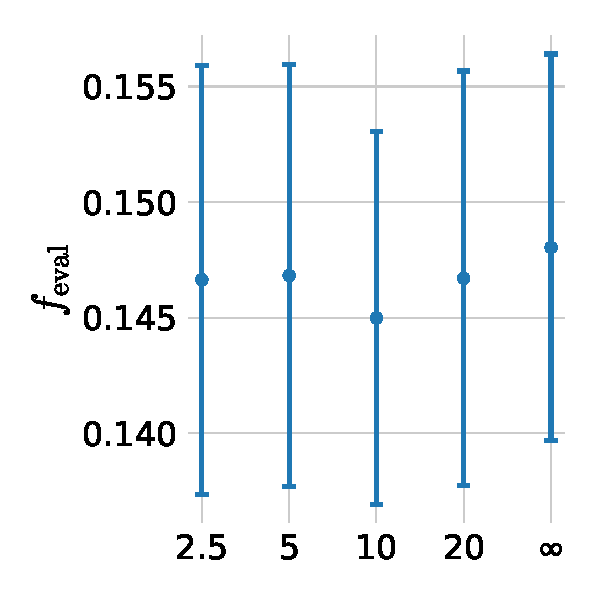
\includegraphics[width=0.95\textwidth, trim=0 0 0 0, clip]{figures/housing/Ejerlejlighed_v19_cut_all_Ncols_all_MAD_gridsearch_half.pdf}
  \caption[Initial HPO Results for the Weight Half-life $T_{\frac{1}{2}}$]
          {Evaluation score as a function of the weight half-life $T_{\frac{1}{2}}$ with the standard deviation over the \num{5} folds as errorbars for apartments.}
  \label{fig:h:hpo_gridsearch_objective}
\end{marginfigure}

\begin{marginfigure}
  \centerfloat
  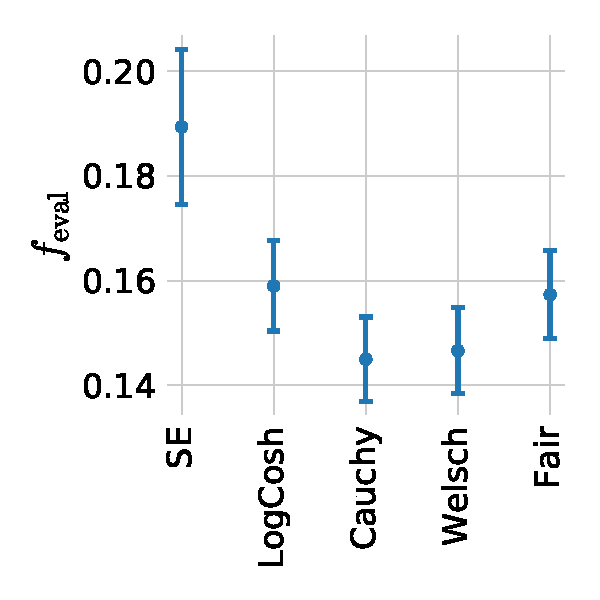
\includegraphics[width=0.95\textwidth, trim=0 0 0 0, clip]{figures/housing/Ejerlejlighed_v19_cut_all_Ncols_all_MAD_gridsearch_obj.pdf}
  \caption[Initial HPO Results for the Loss Function]
          {Evaluation score as a function of the loss function with the standard deviation over the \num{5} folds as errorbars for apartments.}
  \label{fig:h:hpo_gridsearch_halflife}
\end{marginfigure}

For the half-life and the choice of objective function these are shown in Figure~\ref{fig:h:hpo_gridsearch_objective} and \ref{fig:h:hpo_gridsearch_halflife}. In the first of the two figures it is easily seen that even though $T_{\frac{1}{2}}=\SI{10}{\yr}$ is the minimum, the uncertainties are so large that nothing can be concluded definitely with regards to the half-life parameter related to the weights $w(t)$. On the contrary, in the second figure there is a clear performance difference between the different loss functions where the Cauchy loss achieves the best (lowest) value of $f_\mathrm{eval}$ and especially the Squared Error is disregarded. 

The rest of the machine learning models thus continue with the following hyperparameters:

\begin{table}[h]
  \centerfloat
  \begin{tabular}{@{}llcl@{}}
               & $\log_{10}$  & Half-life & Loss function \\ \midrule
  Apartments   & False & \SI{10}{\yr} & Cauchy \\
  Houses       & False & \SI{20}{\yr} & Cauchy
  \end{tabular}
  \label{tab:h:initial_hpo}
\end{table}



\FloatBarrier
\section{Hyperparameter Optimization}
\label{sec:h:hyperparamater_optimization}
With the initial hyperparameter optimization finished, the actual training of the models was started. Again, two XGBoost models were fitted (one for apartments and one for houses) to the training set the hyperparameters were optimized using both random search and Bayesian optimization. These were each run for \num{100} iterations with \num{5}-fold cross validation and early stopping\sidenote{This takes a good \num{4} hours for the random search, \num{7} hours for the Bayesian optimization, and \num{90} minutes to optimize the number of estimators with early stopping for apartments when run on the local computing cluster, HEP. For the houses this takes a good \num{24} hours for the random search, \num{34} hours for the Bayesian optimization, and almost \num{5} hours to optimize the number of estimators with early stopping.}. The hyperparameters to be optimized were the following:
\begin{itemize}
  \item[] The \code{subsample} controls the fraction of row subsampling and is a number between \num{0} and \num{1}. 
  \item[] The \code{colsample_bytree} controls the fraction of column downsampling for each tree, so how many columns (or variables) each tree are allowed to fit to. Is a number between \num{0} and \num{1}.
  \item[] The \code{max_depth} controls the maximum depth of every tree. Is a positive integer (negative values means no maximum depth).  
  \item[] The \code{min_child_weight} variable controls when the decision tree algorithm should stop splitting a node into further nodes (and will thus turn it into a leaf). Is a positive integer.
  \item[] \code{reg_lambda} controls the L2 regularization term. Is a positive number. 
  \item[] \code{reg_alpha} controls the L1 regularization term. Is a positive number.
\end{itemize}

The ranges of the hyperparameters were chosen by a manual, iterative process of fitting a subset of the data (\SI{1}{\percent}--\SI{10}{\percent}) and making sure that the best hyperparameter is not sufficiently close to the boundary of the range; if it is, then the range is extended. The final ranges chosen are shown in Table~\ref{tab:h:hpo_ranges}. Here $\mathcal{U}(a, b)$ refers to a uniform distribution from $a$ to $b$, and $\mathcal{U}_\mathrm{int}(a, b)$ is the same only an integer distribution. 
\begin{margintable}
  \centerfloat
  \begin{tabular}{@{}ll@{}}
  Hyperparameter          &  Range                      \\ \midrule
  \code{subsample}        & $\mathcal{U}(0.5, 0.9)$           \\
  \code{colsample_bytree} & $\mathcal{U}(0.1, 0.99)$           \\
  \code{max_depth}        & $\mathcal{U}_\mathrm{int}(1, 20)$ \\
  \code{min_child_weight} & $\mathcal{U}_\mathrm{int}(1, 30)$ \\
  \code{reg_lambda}       & $\mathcal{U}(0.1, 4)$  \\
  \code{reg_alpha}        & $\mathcal{U}(0.1, 4)$
  \end{tabular}
  % \vspace{\abovecaptionskip}
  \vspace{3mm}
  \caption[PDFs Used in the Random Search]{\label{tab:h:hpo_ranges} Probability Density Functions used in the random search to draw new sets of values for the hyperparameters. Each hyperparameter is drawn from the distribution seen in the table.}
\end{margintable}

The fitting pipeline from this point on consists of first running both random search and Bayesian optimization. Their results are compared and the best of the two models is chosen. Finally, this model is re-fitted with early stopping where the learning rate $\eta$ is reduced from $\eta=0.1$ to $\eta=0.01$. In the end, one ends up with a model that has been hyperparameter optimized for preprocessing optimizations, loss functions, sample weights, normal XGB hyperparameters and finally the number of estimators. I have manually implemented this pipeline in Python since no other packages provide the same flexibility as a custom implementation that works fully automated. The results of the random search and the Bayesian optimization are shown in Figure~\ref{fig:h:CV_res_RS_parallel_coords_ejer_non_appendix} and \ref{fig:h:CV_res_BO_parallel_coords_ejer}. The corresponding plots for houses are shown in Figure~\ref{fig:h:CV_res_RS_parallel_coords_villa} and \ref{fig:h:CV_res_BO_parallel_coords_villa}. 

\begin{figure*}
  \centerfloat
  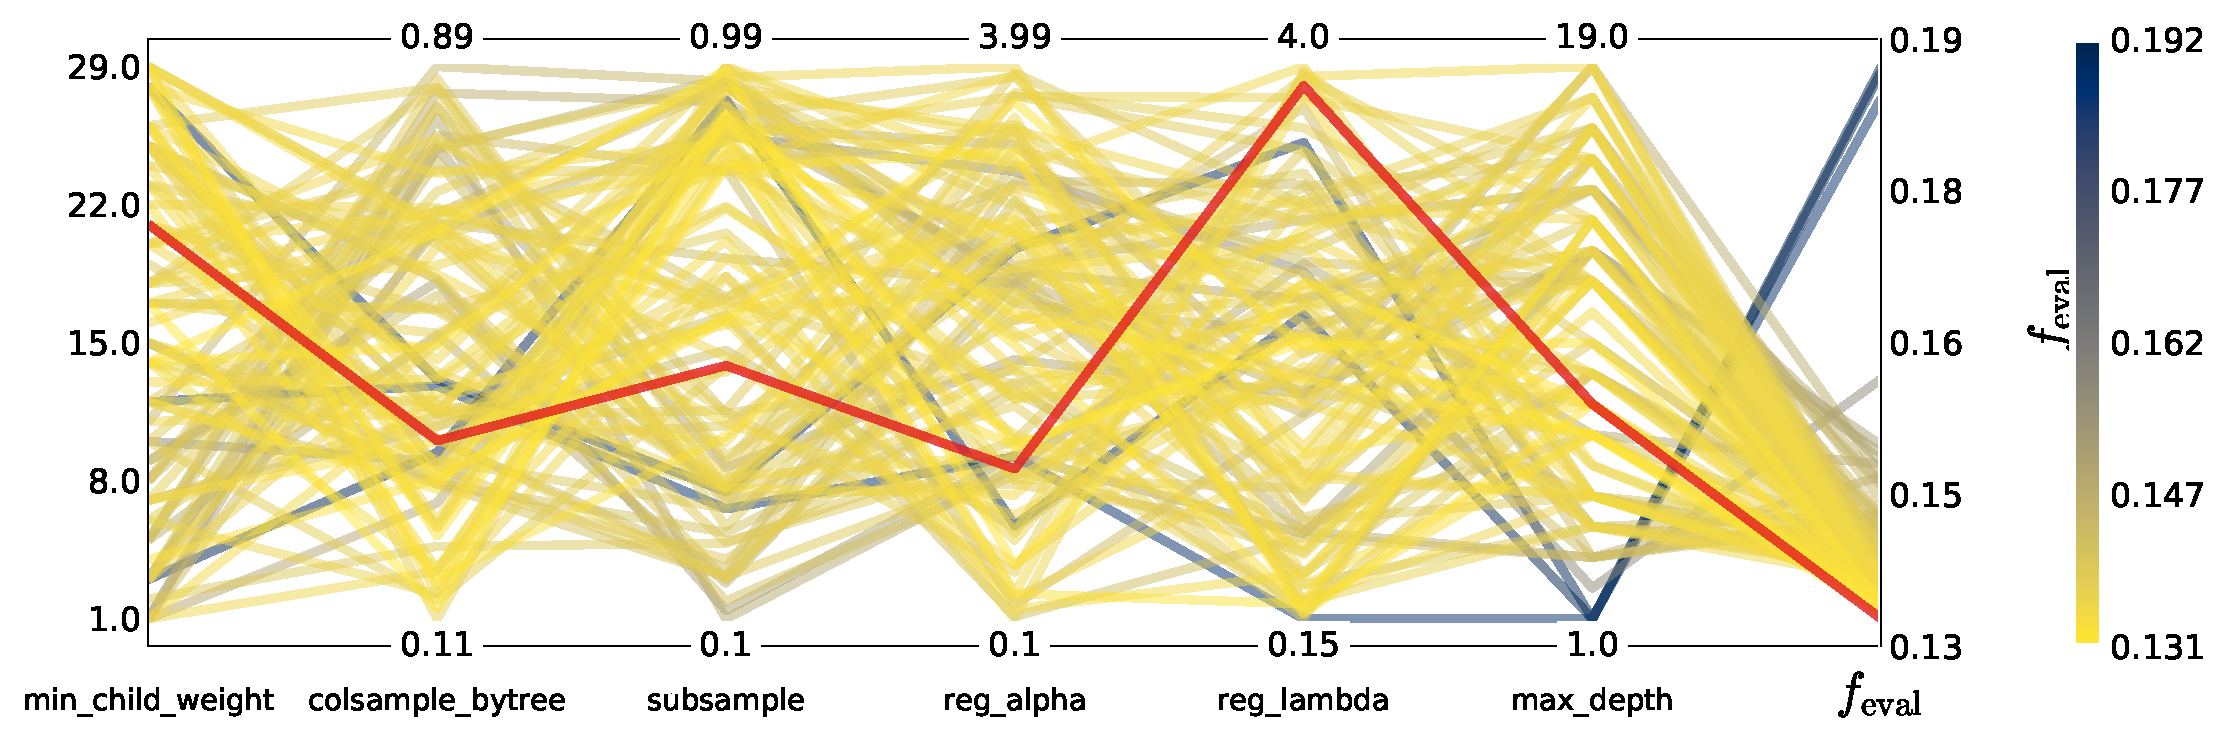
\includegraphics[width=0.99\textwidth, trim=0 0 0 0, clip]{figures/housing/Ejerlejlighed_v19_cut_all_Ncols_all_CV_viz_HPO_RS.pdf}
  \caption[Parallel Coordinate Plot of the Random Search Hyperparameter Optimization Results of XGBoost for Apartments]
          {Hyperparameter optimization results of XGBoost parameters of the housing model for apartments shown as parallel coordinates. Here shown for random search. } 
  \label{fig:h:CV_res_RS_parallel_coords_ejer_non_appendix}
\end{figure*}

As with the initial grid search, it is important to compare the results in Figure~\ref{fig:h:CV_res_RS_parallel_coords_ejer_non_appendix} with their uncertainties. Figure~\ref{fig:h:CV_res_RS_uncertainties_ejer} shows the value of the evaluation function along with its \num{1}$\sigma$  and \num{2}$\sigma$ uncertainties are plotted as a function of the iteration along the $x$-axis. The minimum value of $f_\mathrm{eval}$ is shown in red. Even though this is the minimum value, notice how most of the other iterations are within \num{1}$\sigma$. The plot for the Bayesian optimization in Figure~\ref{fig:h:CV_res_BO_uncertainties_ejer} shows the exploration phase in the first half of the iterations where it afterwards converge to a more flat minimum, however, this minimum was still worse than the one found with random search. 

\begin{figure}
  \centerfloat
  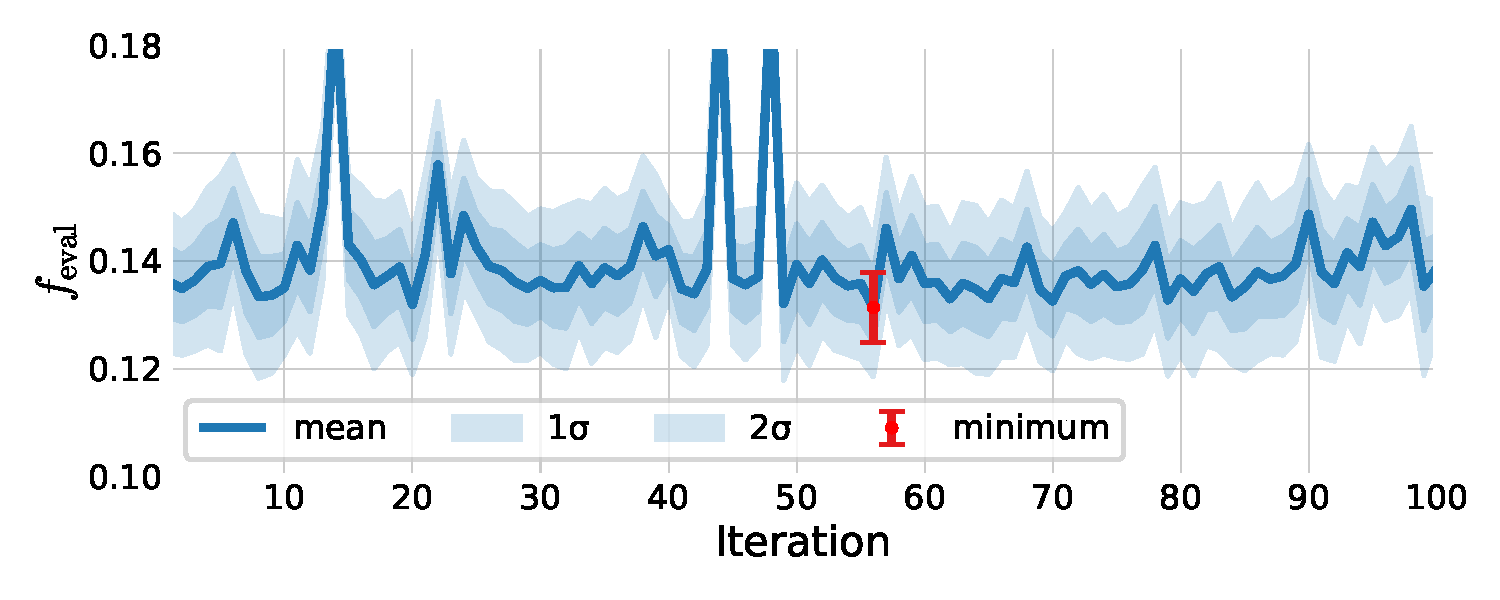
\includegraphics[width=0.95\textwidth, trim=10 20 10 10, clip]{figures/housing/Ejerlejlighed_v19_cut_all_Ncols_all_xgb_score_over_time_random.pdf}
  \caption[Hyperparameter Optimization: Random Search Results]
          {The results of running random search on apartments using the XGB-model. The \textcolor{red}{minimum (mean) loss} along with its uncertainty is shown in red, the \textcolor{blue}{means} for the different iterations of random search in blue, and as light blue bands are the \textcolor{blue}{one (and two) standard deviation(s)}, all as a function of iteration number.} 
  \label{fig:h:CV_res_RS_uncertainties_ejer}
\end{figure}

% The best of the random search and the Bayesian optimization models is chosen for the subsequent analysis by first reducing the learning rate to $\eta=0.01$ and then find the best number of estimators by early stopping. 
The evaluation function as a function of number of estimators, also known as the \emph{learning curve}, is shown in Figure~\ref{fig:h:CV_res_ES_learning_curve_ejer} for the combined early stopping model. This curve is the realization of the theoretical Figure~\ref{fig:ml:empirical_risk} in real data, where it first improves a lot and then finds a stable plateau, although it slowly increases. The minimum and its uncertainty are shown in red. To reduce the model complexity (with the further advantage of resulting in a faster model at prediction time) we keep the model with the lowest number of estimators that are still within $1\sigma$ of the minimum: see the orange point in the figure. This results in a model that contains less than a fifth of the number of trees and is thus also significantly simpler and faster at inference time. This is the final hyperparameter optimized model that will be used for the further analysis. 

\begin{figure}
  \centerfloat
  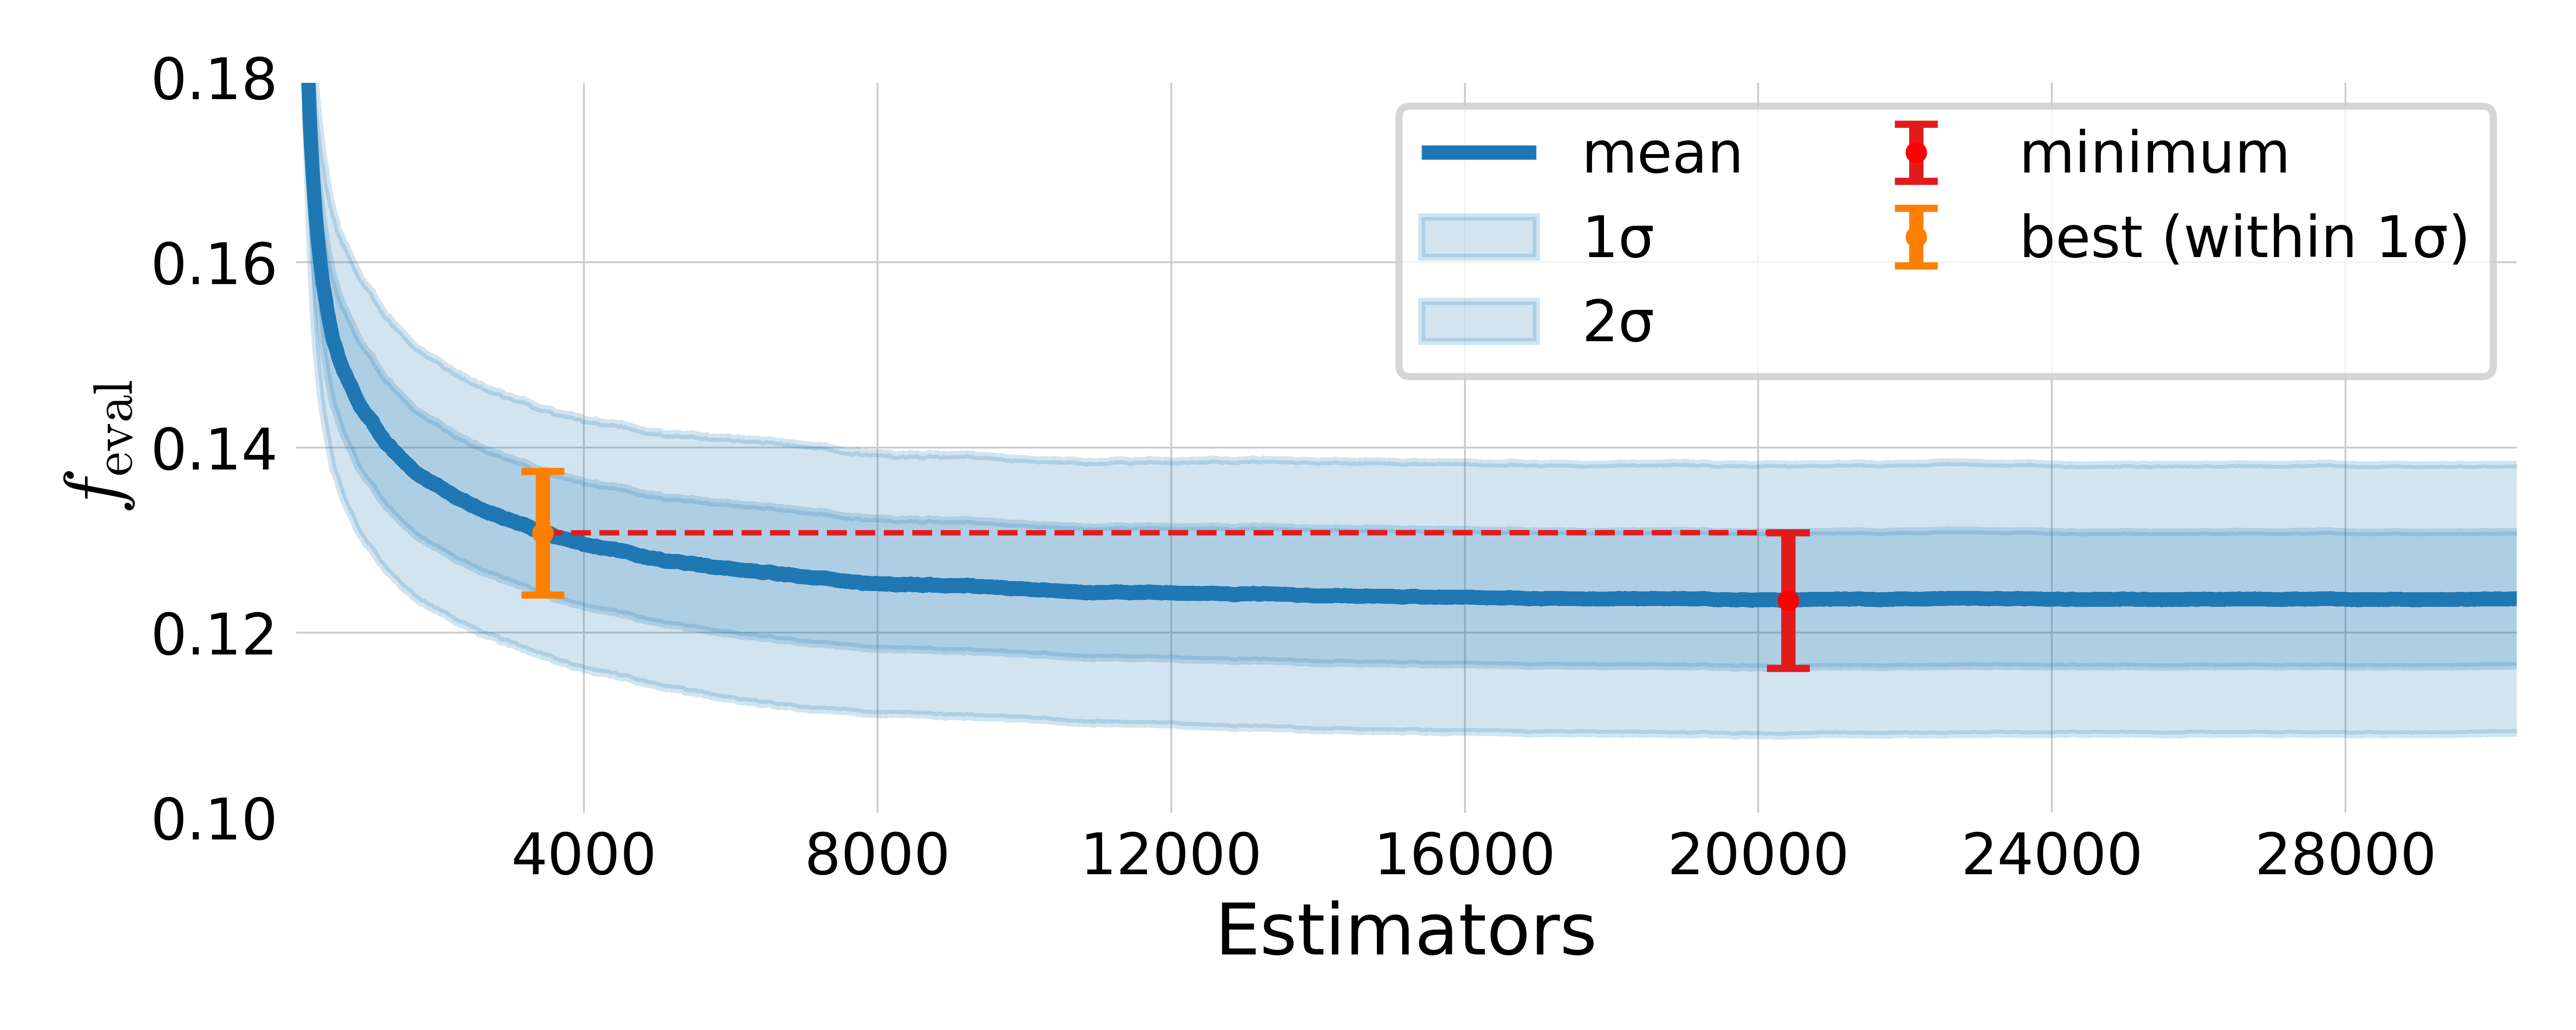
\includegraphics[draft=false, width=0.99\textwidth, trim=10 20 10 10, clip]{figures/housing/Ejerlejlighed_v19_cut_all_Ncols_all_xgb_early_stopping_fig.png}
  \caption[Early Stopping Results]
          {The results of early stopping on apartments using the XGB-model. The \textcolor{red}{minimum (mean) loss} along with its uncertainty is shown in red, the \textcolor{blue}{means} for the different iterations of random search in blue, and as light blue bands are the \textcolor{blue}{one (and two) standard deviation(s)}, all as a function of number of estimators (trees). In orange the \textcolor{orange}{\q{best} number of estimators} is shown, defined as the lowest number of estimators which are still within $1\sigma$ of the minimum value.} 
  \label{fig:h:CV_res_ES_learning_curve_ejer}
\end{figure}

\vspace{-0.5cm}


\FloatBarrier
\section{Results}
\label{sec:h:results}

The performances of the three different models (the RS-optimized, the BO-optimized and the best of the two optimized with early stopping) are shown in Figure~\ref{fig:h:CV_res_performance_ejer}. Here the distribution of the relative price prediction $\vec{z}$ of the test set is shown for the three models. In addition to the distributions, also the performance metrics are shown: the value of the evaluation function\sidenote{Written as \code{MAD}.} along with the fraction of relative price predictions that are within the specified percentage. In this particular instance it is seen that \SI{41.3}{\percent} of the predictions by the final early stopping model are less than $\pm\SI{5}{\percent}$ wrong, \SI{69.8}{\percent} within $\pm\SI{10}{\percent}$, and \SI{91.9}{\percent} within $\pm\SI{20}{\percent}$. Note that the differences between the three models are minor and that the distributions almost cannot be distinguished from each other. 

\begin{figure*}[h!]
  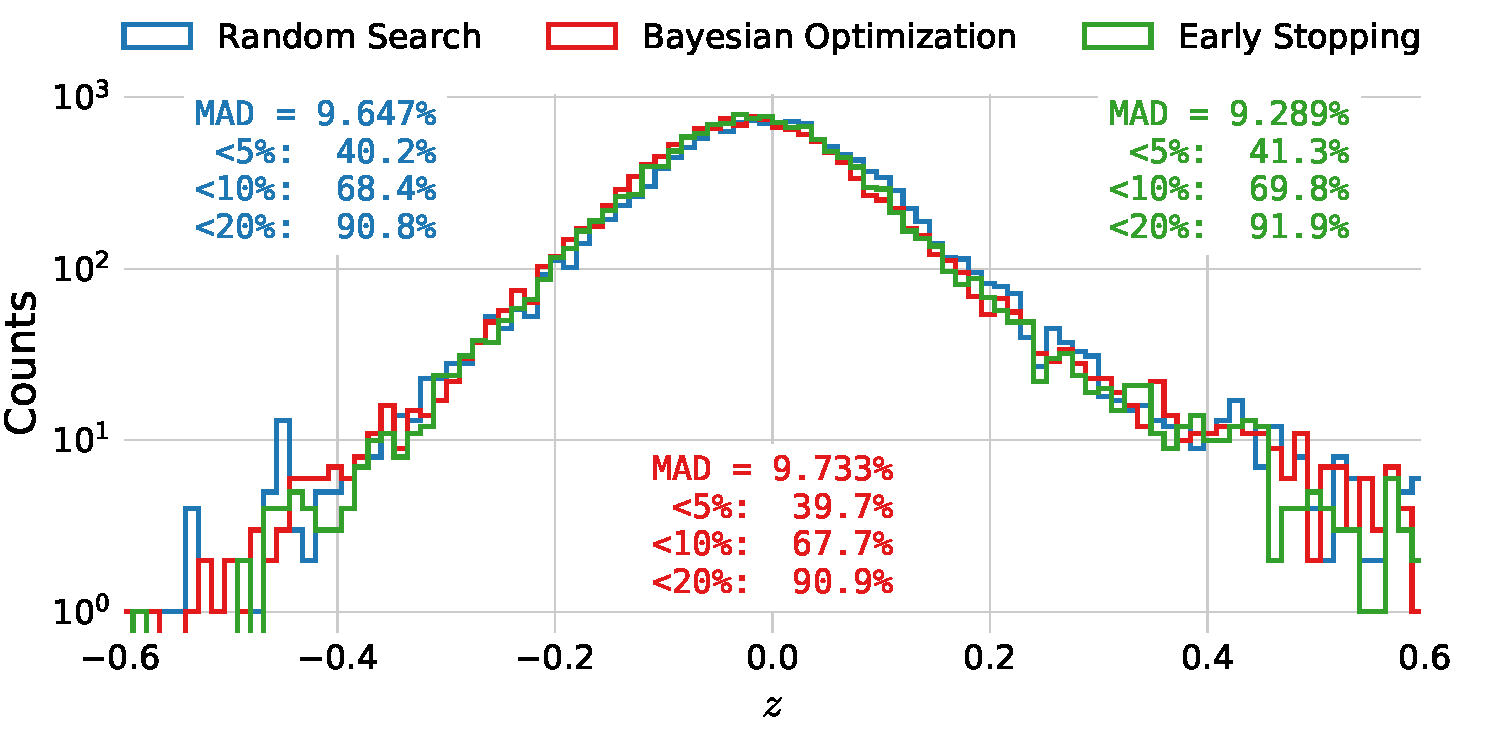
\includegraphics[width=0.95\textwidth, trim=0 10 10 5, clip]{figures/housing/Ejerlejlighed_v19_cut_all_Ncols_all_xgb_z_hist_metrics.pdf}
  \caption[Performance of XGB-model for Apartments]
          {Histogram of $z$-values of the XGB-model trained on apartments. The performance after hyperparameter optimization using \textcolor{blue}{random search} is shown in blue, for \textcolor{red}{Bayesian optimization} in red, and the final model which is optimized with \textcolor{green}{early stopping} in green.
          } 
  \label{fig:h:CV_res_performance_ejer}
\end{figure*}

An interesting observation from the performance metrics of the test set is the low value of $f_\mathrm{eval}=\SI{9.289}{\percent}$ (\code{MAD}). By looking at Figure~\ref{fig:h:CV_res_ES_learning_curve_ejer}, one would expect a test loss of around \SI{12}{\percent} assuming iid. samples. However, this assumption does not seem to be fulfilled for the test set. The performances of the realtors are also better for the test set than the training set, and by comparing the test set with the extra \num{2019} set, it seems to be \num{2018} that was an extra homogenous year. The realtors' performance is shown in Table~\ref{tab:h:realtor_mad_train_test_2019} for apartments and in Table~\ref{tab:h:realtor_mad_train_test_2019_houses} for houses. The \q{Tight} in the the table corresponds to the realtors performance on the tight versions of the different datasets. The performance of the XGB models on the tight test set is shown in Figure~\ref{fig:h:CV_res_performance_ejer_tight}. 
\begin{margintable}[-0.5cm]
  \centerfloat
  \begin{tabular}{@{}rlll@{}}
          & Train               & Test                & \num{2019}          \\ \midrule
  Normal  & \SI{5.80}{\percent} & \SI{4.97}{\percent} & \SI{6.19}{\percent} \\
  Tight   & \SI{5.69}{\percent} & \SI{4.94}{\percent} & \SI{6.19}{\percent} 
  \end{tabular}
  \vspace{2mm}
  \caption[Realtors' MAD for apartments]{The $\mathrm{MAD}_0$ of the realtors' predictions for the normal and tight selections of apartments in the training, test, and \num{2019} datasets.}
  \label{tab:h:realtor_mad_train_test_2019}
\end{margintable}
\begin{margintable}[0.1cm]
  \centerfloat
  \begin{tabular}{@{}rlll@{}}
          & Train               & Test                & \num{2019}          \\ \midrule
  Normal  & \SI{12.25}{\percent} & \SI{7.89}{\percent} & \SI{8.49}{\percent} \\
  Tight   & \SI{11.62}{\percent} & \SI{7.59}{\percent} & \SI{8.07}{\percent} 
  \end{tabular}
  \vspace{2mm}
  \caption[Realtors' MAD for houses]{The $\mathrm{MAD}_0$ of the realtors' predictions for the normal and tight selections of houses in the training, test, and \num{2019} datasets.}
  \label{tab:h:realtor_mad_train_test_2019_houses}
\end{margintable}

The results for the final model are shown in Table~\ref{tab:h:results_ejer} for owner-occupied apartments and in in Table~\ref{tab:h:results_villa} for one family houses. The $\mathrm{MAD}_0$ is around \SI{9}{\percent} for apartments and \SI{16}{\percent} for houses, which is still worse than the realtors' predictions, yet still acceptable for a model that does not have any variables describing the indoor conditions. For apartments around \SI{40}{\percent} of all the predictions are within $\pm \SI{5}{\percent}$ and more than \SI{90}{\percent} are within $\pm \SI{20}{\percent}$ which is similar to the performance of the professional, automated property evaluations from e.g. \citet{bolighedBolighedUsikkerhedDatavurderingen}. The performances on the tight cuts are shown in Table~\ref{tab:h:results_ejer_tight} and \ref{tab:h:results_villa_tight}. 

\begin{table}
  \centerfloat
  \begin{tabular}{@{}lcccc@{}}
    {} &      $\mathrm{MAD}_0$ (\%) & $\leq 5\% (\%)$ &  $\leq 10\% (\%)$ &   $\leq 20\% (\%)$   \\
    \midrule
    Train & \num{7.83} & \num{47.90} & \num{75.74} & \num{93.97} \\
    Test  & \num{9.29} & \num{41.33} & \num{69.77} & \num{91.91} \\
    2019  & \num{9.89} & \num{38.85} & \num{66.76} & \num{90.04}    
  \end{tabular}
  \caption[Performance Metrics for Apartments]{Performance metrics for the final housing model trained and evaluated on apartments.}
  \label{tab:h:results_ejer}
\end{table}


\begin{table}
  \centerfloat
  \begin{tabular}{@{}lcccc@{}}
    {} &      $\mathrm{MAD}_0$ (\%) & $\leq 5\% (\%)$ &  $\leq 10\% (\%)$ &   $\leq 20\% (\%)$    \\
    \midrule
    Train & \num{14.12} & \num{28.95} & \num{51.89} & \num{78.04}  \\
    Test  & \num{15.79} & \num{25.61} & \num{47.52} & \num{75.14}  \\
    2019  & \num{16.50} & \num{24.01} & \num{45.89} & \num{74.22}     
  \end{tabular}
  \caption[Performance Metrics for Houses]{Performance metrics for the final housing model trained and evaluated on houses.}
  \label{tab:h:results_villa}
\end{table}



\section{Forecasting}
\label{sec:h:forecasting}

To gauge the predictive power of the final model over time, we predicted prices of the following month's sales and compared the predictions to the actual, sold prices. This is done on a month-by-month basis for all the months in the test set (\num{2018}) and \num{2019}. 
We applied two different methods of forecasting: \emph{static} forecasting where the model is only trained once, and \emph{dynamic} forecasting where the model is retrained after each month on all of the previous sales. These predictions allow the relative predictions $\vec{z}$ to be calculated and the $\mathrm{MAD}_0$ and the standard deviation (SD) of $\vec{z}$ are shown in Figure~\ref{fig:h:forecast_MAD_SD}. 
\begin{figure}
  \centerfloat
  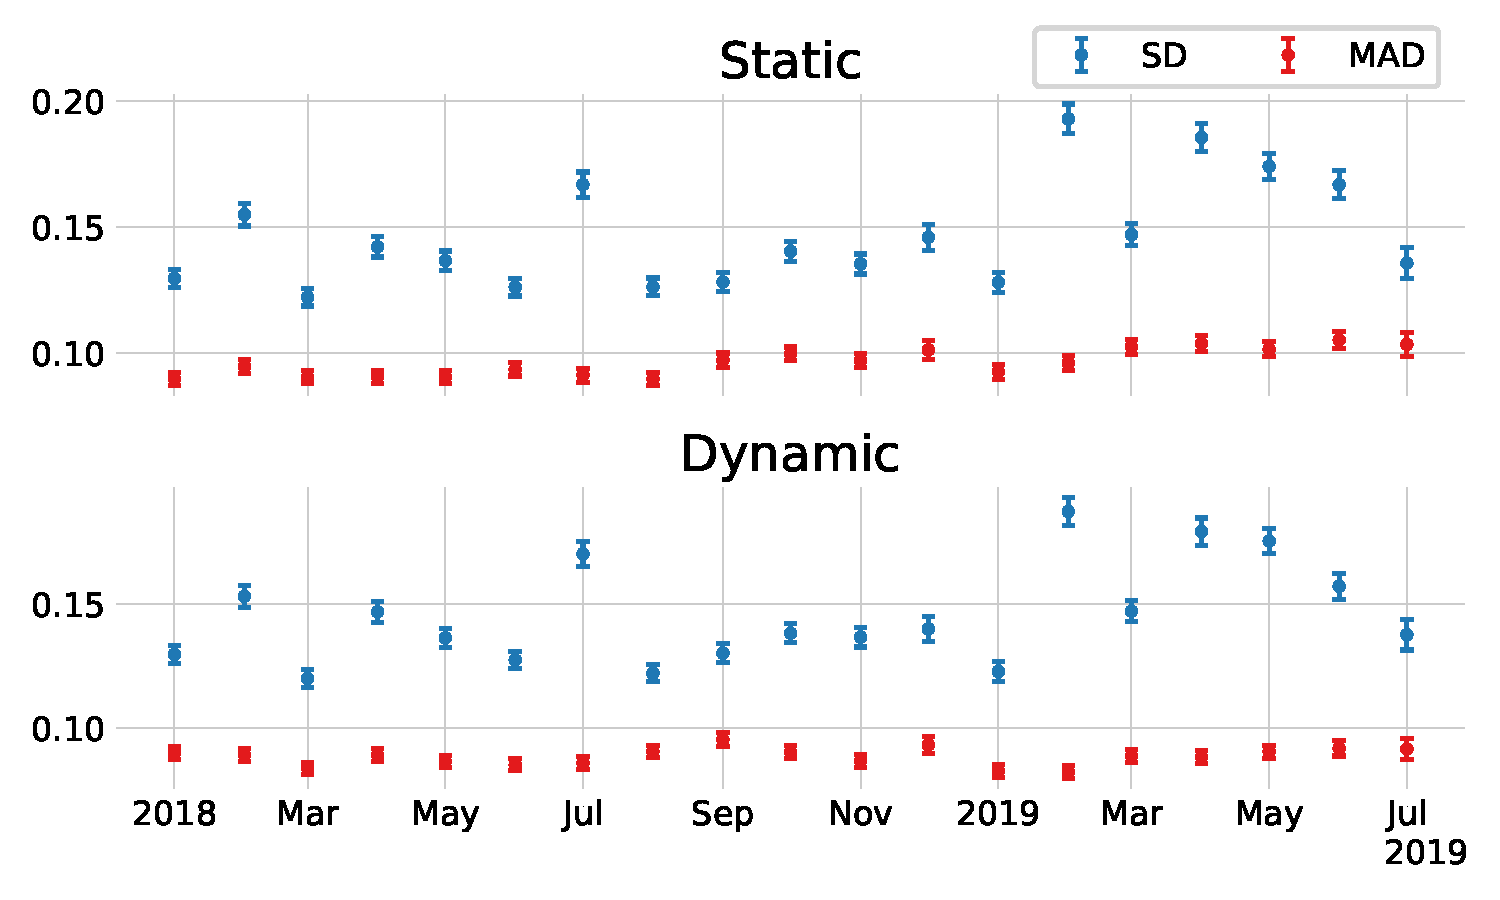
\includegraphics[width=0.99\textwidth, trim=10 15 10 10, clip]{figures/housing/Ejerlejlighed_v19_cut_all_Ncols_all_xgb_forecast_prediction_MAD.pdf}
  \caption[Standard Deviation and MAD of the Static and Dynamic XGB Forecasts]
          {Performance of 1-month forecasts for apartments sold in \num{2018} and \num{2019}. For both plots the XGB model is trained on data up to (but excluding) 2018. Top) The performance of the static model's prediction for both the \textcolor{blue}{standard deviation (SD)} and \textcolor{red}{$\mathrm{MAD}_0$} of the $z$-scores. Bottom) Same as above, however, based on a dynamic model, i.e. a model which is retrained after every month to include the previous month's sales.} 
  \label{fig:h:forecast_MAD_SD}
\end{figure}

In the top subplot the results for the static forecast are shown, whereas the dynamic results are shown in the bottom subplot. The errorbars are calculated using the usual variance of the standard deviation:
\begin{equation}
  \sigma_\mu  = \frac{\sigma}{\sqrt{N}}, \quad \sigma_\sigma = \frac{\sigma}{\sqrt{2N}},
\end{equation}
where $\sigma_\mu$ is the standard deviation of the mean and $\sigma_\sigma$ is the standard deviation of the standard deviation\sidenote{That this estimator is biased does not matter since we are in the large $N$ limit, $N \sim 1000$.} \autocite{Barlow:0471922951}.
Notice the large fluctuations in the standard deviations over time compared to the $\mathrm{MAD}_0$s which is an effect of $\mathrm{MAD}_0$ being a robust estimator. What is also interesting to note is that the $\mathrm{MAD}_0$ seems to increase over time for the static model, albeit slowly. In comparison, for the dynamic model this seem less pronounced. This figure not only shows the time dependence of the performance of the model, but also that the model is quite stable over time, at least for the dynamic model. 

Using the relative price predictions $\vec{z}$, we construct the Market Index, $\mathrm{MI}$. This is an index which measures the overall level of the Danish housing market based on the assumption that if the houses sold in a month are generally sold at a higher price than was predicted by the model, there can be two reasons for it: either the model was wrong or the market simply changed in the time span. With the latter assumption, the ratio between the prediction and the actual price of a residence is thus a measure of the market index:
\begin{equation}
  \begin{split}
    z_\mathrm{mi} &\equiv \frac{\hat{y}}{y} = 1 - \frac{\hat{y}-y}{y}  = 1-z \\
    \mathrm{MI}_\mathrm{mean} &= \mathrm{mean}(\vec{z}_\mathrm{mi}) \\
    \mathrm{MI}_\mathrm{median} &= \mathrm{median}(\vec{z}_\mathrm{mi}).
    \label{eq:h:market_index}
  \end{split}
\end{equation}
Here $\vec{z}_\mathrm{mi}$ is the vector of ratios between prediction and actual price, and the market index can then be estimated using either the mean $\mathrm{MI}_\mathrm{mean}$ or the median $\mathrm{MI}_\mathrm{median}$. 

Figure~\ref{fig:h:forecast_MarketIndex} shows the market indices on a monthly basis for the static and the dynamic models. In the top panel the market index is shown for the static model. Here the median $\mathrm{MI}_\mathrm{median}$  is consistently higher than \num{1}, around \SI{1}{\percent}. Compare this to the dynamic $\mathrm{MI}_\mathrm{median}$ in the lower plot which fluctuates around \num{1}. The mean $\mathrm{MI}_\mathrm{mean}$ is added to show that its fluctuations are higher than the medians. 
\begin{figure}
  \centerfloat
  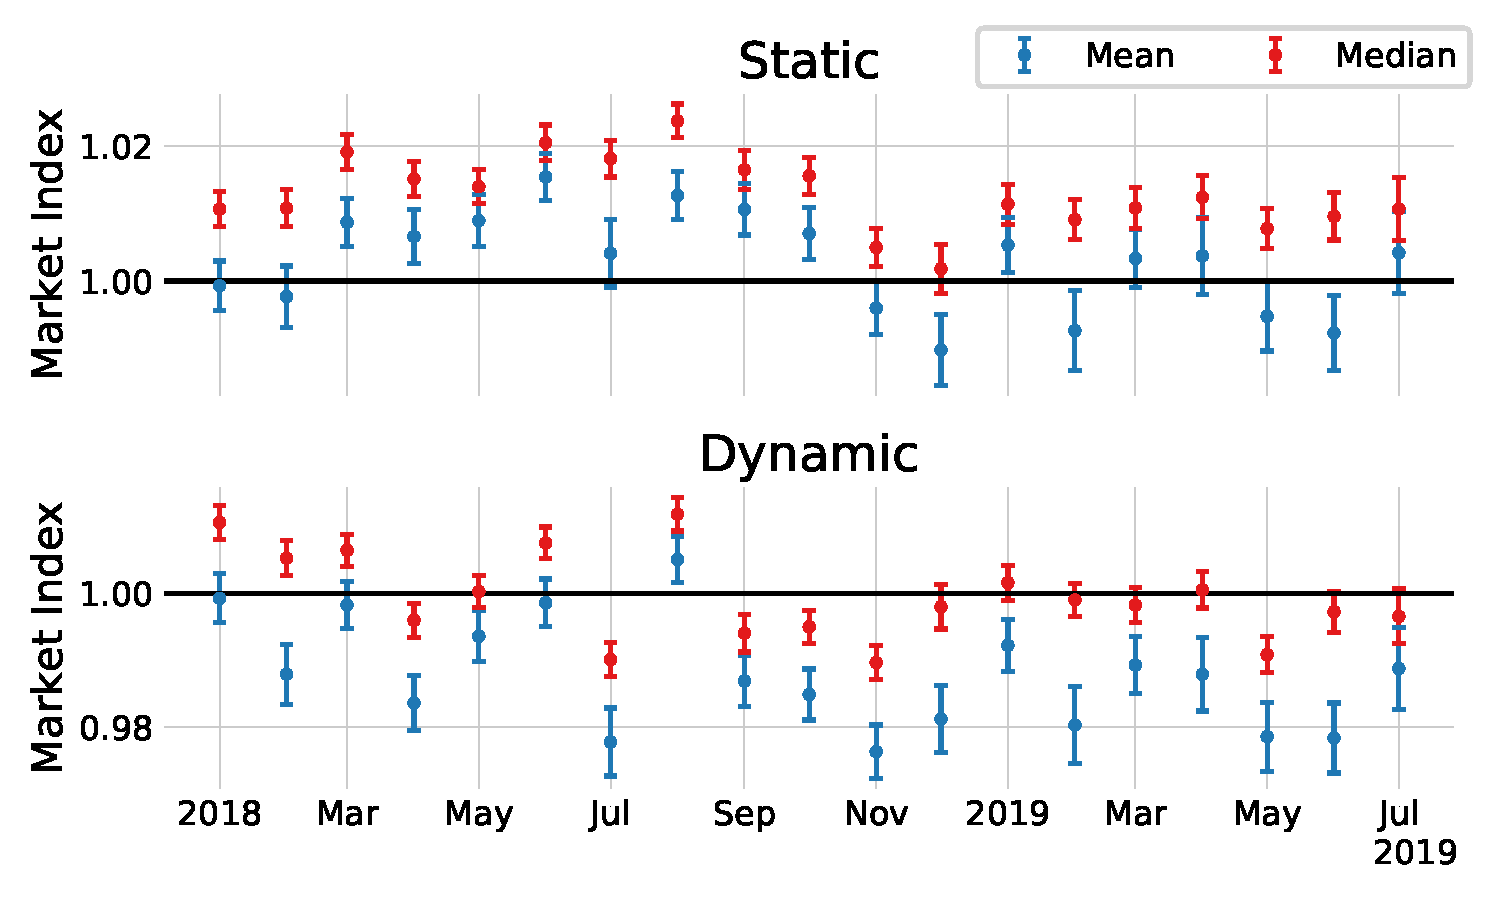
\includegraphics[width=0.99\textwidth, trim=10 15 10 10, clip]{figures/housing/Ejerlejlighed_v19_cut_all_Ncols_all_xgb_forecast_prediction_MarketIndex.pdf}
  \caption[Market Index based on the Static and Dynamic XGB Forecasts]
          {The Market Index as defined in equation \eqref{eq:h:market_index} for the static and dynamic 1-month forecasts for \num{2018} and \num{2019}. The \textcolor{red}{mean} is plotted in red and the \textcolor{blue}{median} in blue.} 
  \label{fig:h:forecast_MarketIndex}
\end{figure}

\FloatBarrier
\section{Model Inspection}
\label{sec:h:model_inspection}

As mentioned previously, one of the most important aspects of advanced machine learning methods (in addition to getting accurate predictions) is to understand the model. As mentioned in \autoref{sec:ml:feature_importance}, it is possible to use SHAP values to inspect the trained model for both local predictions and for global feature importances $\phi_i^\mathrm{tot}$. An example of how to use SHAP to better understand a local prediction is shown in Figure~\ref{fig:h:shap_single_apartment}. In this figure, I visualize the SHAP values for a particular sale as a bar chart and compare it to the final prediction $\hat{y}$. Remember, for SHAP values the prediction is the sum of all of the SHAP values. The expectation value is denoted as \code{Bias} in the plot. To show all \num{143} variables would make the figure excessively large, so two extra bins have been added: the \code{Overflow} bar which is the sum of the remaining positive SHAP values and likewise with \code{Underflow} for negative values. The sum of all the green and red bars adds up to $\hat{y}=\SI{6.86}{\Mkr}$ in this particular instance and the actual sold value was $y=\SI{6.35}{\Mkr}$ Thus, in cases where there is a large discrepancy between the predicted and actual sales prices, one can use this tool to better understand why the prediction was estimated as it was. 

\begin{figure*}[ht!]
  \centerfloat
  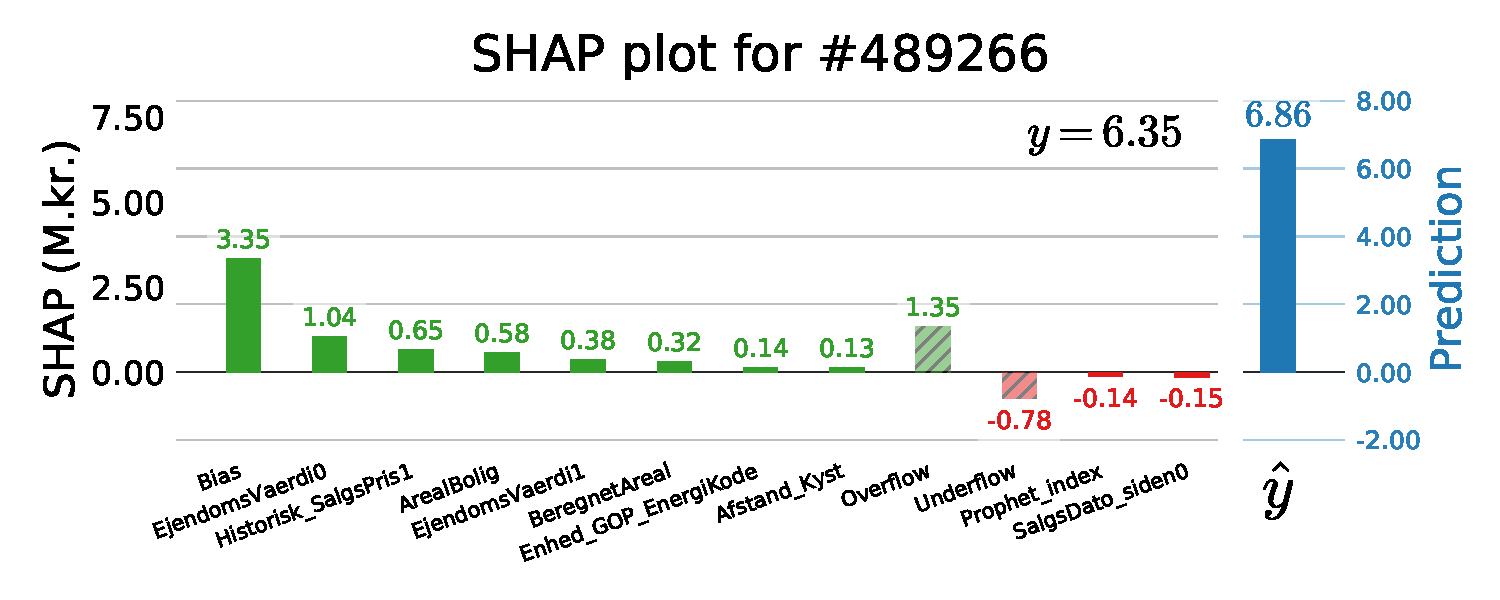
\includegraphics[width=0.99\textwidth, trim=15 15 10 40, clip]{figures/housing/Ejerlejlighed_v19_cut_all_Ncols_all_SHAP_fig_loc=489266.pdf}
  \caption[SHAP Prediction Explanation for Apartments]
          {Model explanation for XGB model for a specific apartment. The bars are the variables in the dataset that the model found most important sorted after their importance for this particular apartment. The bias bar refers to the expected value of the model, which is simply the mean of the training set which acts as the naive prediction baseline. The \q{cutoff positive (negative)} bars are the sum of the remaining positive (negative) values that are not shown. On the right hand side of the plot is the model prediction shown. The model prediction is the sum of all of the bars in the left par (\SI{6.86}{\Mkr} in this example). The \textcolor{red}{negative} values are shown in red, \textcolor{green}{positive} ones in green, and the \textcolor{blue}{prediction value} in blue. 
          } 
  \label{fig:h:shap_single_apartment}
\end{figure*}

Figure~\ref{fig:h:shap_overview} shows which variables are most important on a global scale as measured by $\phi_i^\mathrm{tot}$. Here the variables are sorted according to the normalized $\phi_i^\mathrm{tot}$ which is shown in parentheses after each variable name. In the center of the plot is shown a dot-plot of the dataset plotted with the SHAP value on the $x$-axis and colored according to the feature value. 

The way to interpret this plot is as follows. Take a variable of interest, e.g. the area of the apartment \code{ArealBolig} with $\phi_\mathrm{ArealBolig}^\mathrm{tot}=\SI{5.35}{\percent}$. Every dot is a sale plotted as a function of their SHAP value with a spread such that the height corresponds to the SHAP distribution of that specific feature. For the area, it can be seen that there is a long tail towards high SHAP values, however, most of the samples have slightly negative SHAP values. The dots are colored according to their feature value and it can thus be seen that large apartments (red) are given a higher SHAP value than small apartments (blue); precisely as expected from the model. In contrary, when the total days on market (\code{LiggetidSamlet}) is large it pushes the prediction in the negative direction. 

\begin{figure}[ht!]
  \centerfloat
  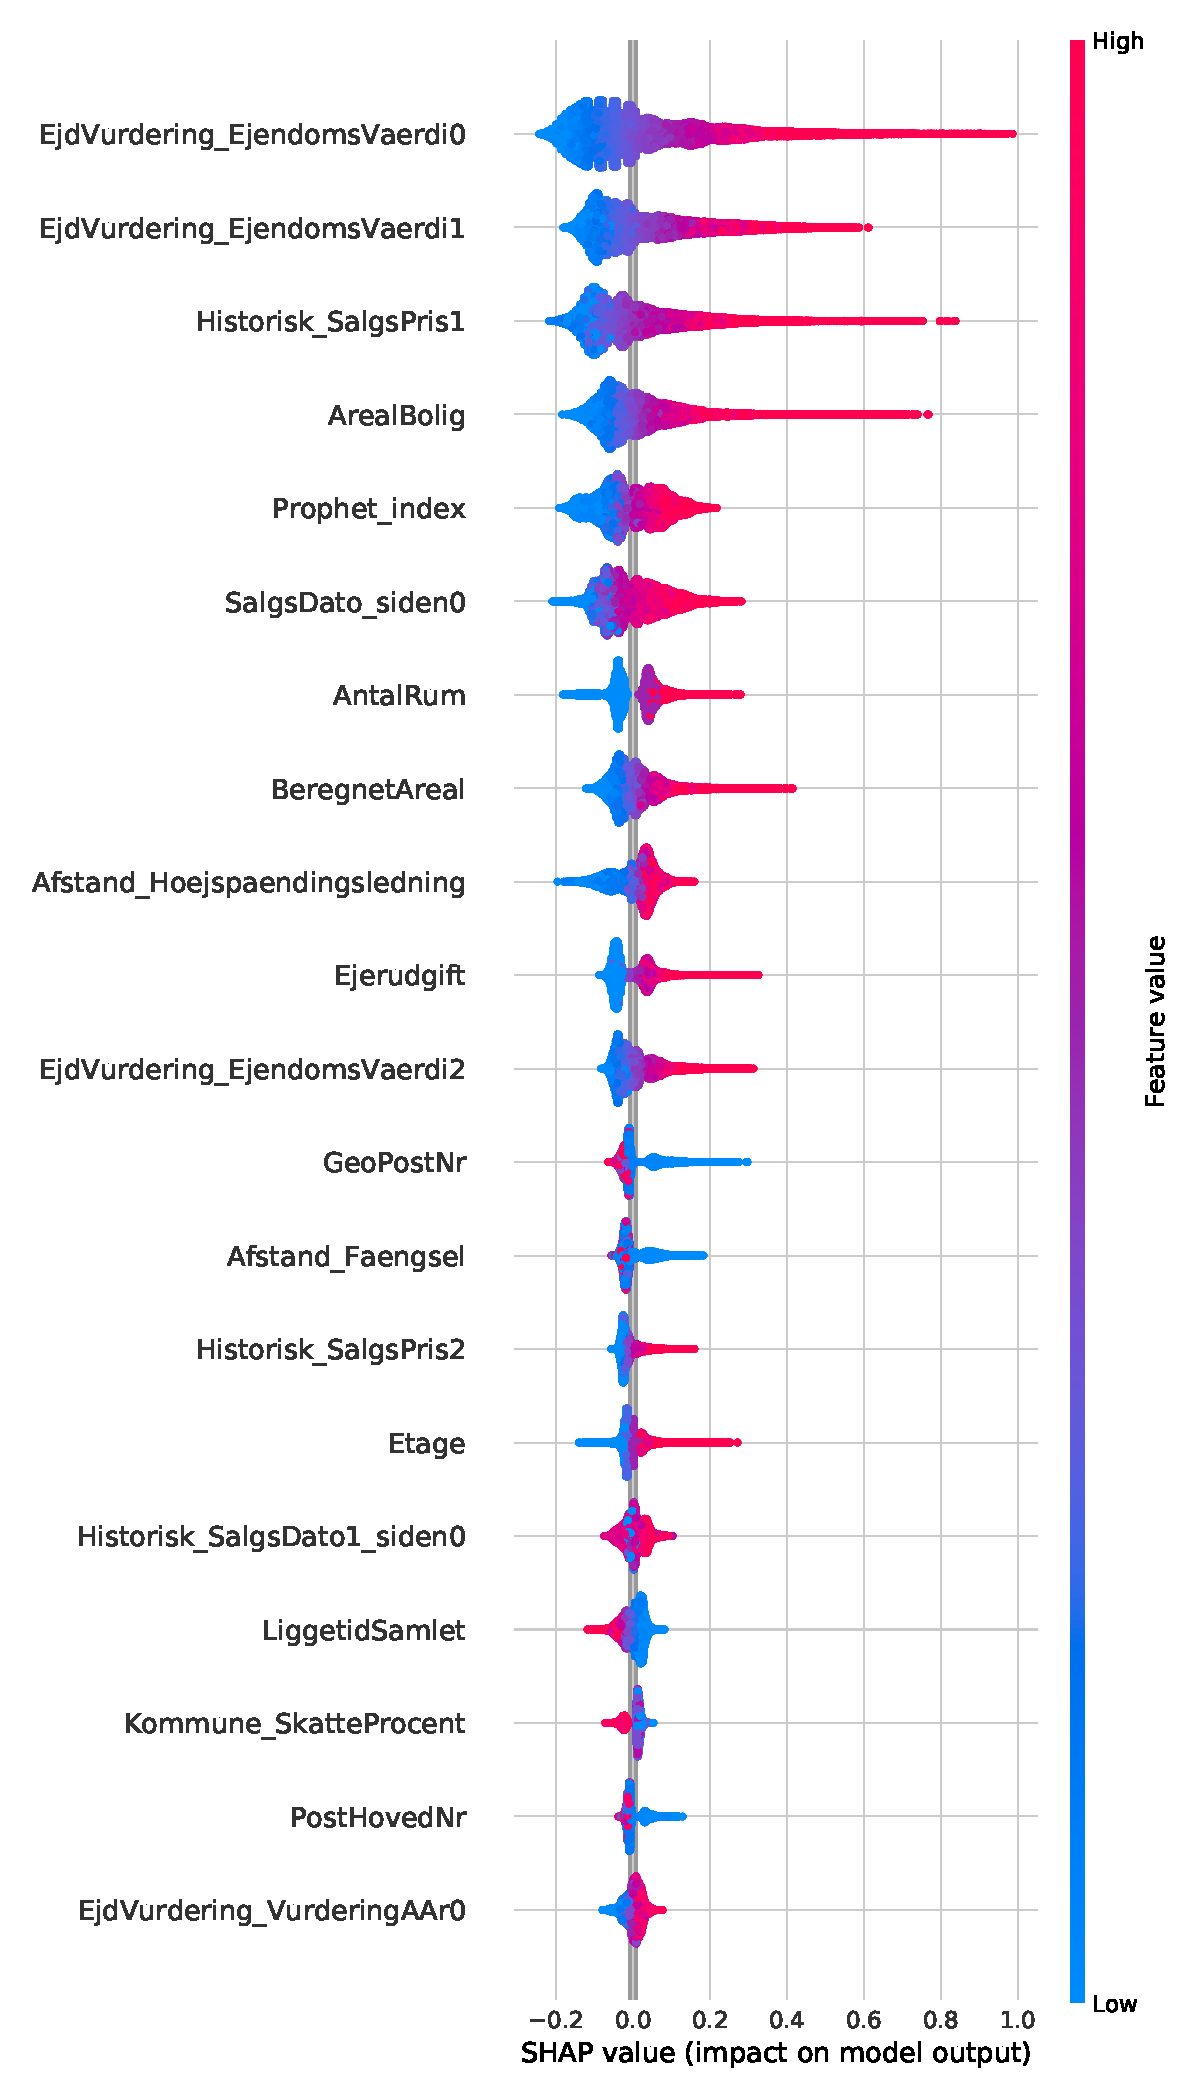
\includegraphics[width=0.9\textwidth, trim=0 0 0 1, clip]{figures/housing/Ejerlejlighed_v19_cut_all_Ncols_all_xgb_tight_SHAP_vals_summary.pdf}
  \caption[Feature importance of Apartments Prices]
          {Feature importance of apartment prices using the XGB-model. The feature importance is measured using SHAP values. The variables are sorted top to bottom according to their overall feature importance, i.e. the previous public property valuation \code{EjendomdsVaerdi0} is the most important single feature. Along the $x$-axis is the impact on model output, in this example the price in \si{\Mkr} This axes is colored by the value of the feature, from \textcolor{blue}{low} (blue) to \textcolor{red}{high} (red). In this particular example we see that high values of the previous public property valuation has high, positive impact on the model prediction -- exactly as expected. This is exactly opposite the total days on market described by the variable \code{LiggetidSamlet} where a high value has a negative impact.  
          } 
  \label{fig:h:shap_overview}
\end{figure}

The SHAP software \citep{lundbergConsistentIndividualizedFeature2018} not only allows for 1D dependencies to be gauged, it also features the so-called \emph{interaction plots}. These plots show the 2D-dependence between the variable and the SHAP value colored according to a second variable. Since the previous public property valuation (PPPV) (\code{EjendomdsVaerdi0}) is the most important of the features, the interaction plot of this variable is seen in Figure~\ref{fig:h:shap_overview_interaction}. Here the SHAP value (of the \code{EjendomdsVaerdi0}) is plotted as a function of \code{EjendomdsVaerdi0}. This plot shows that the higher the PPPV, the higher the model output. The colors show how this trend depends on time by the variable \code{SalgsDato_siden0} which is the number of days since January \nth{1} 2009 that the apartment was sold. The plots shows that newer sales with a high PPPV has even higher SHAP values than older sales with the same high PPPV. This agrees with the fact that the market has gone up since 2009. On the other hand, for low PPPV apartments the relationship with time is opposite, however, the effect is much smaller here. The SHAP software chose to color by \code{SalgsDato_siden0} since this is the variable which explains most of the variation for a given PPPV. 

\begin{figure}
  \centerfloat
  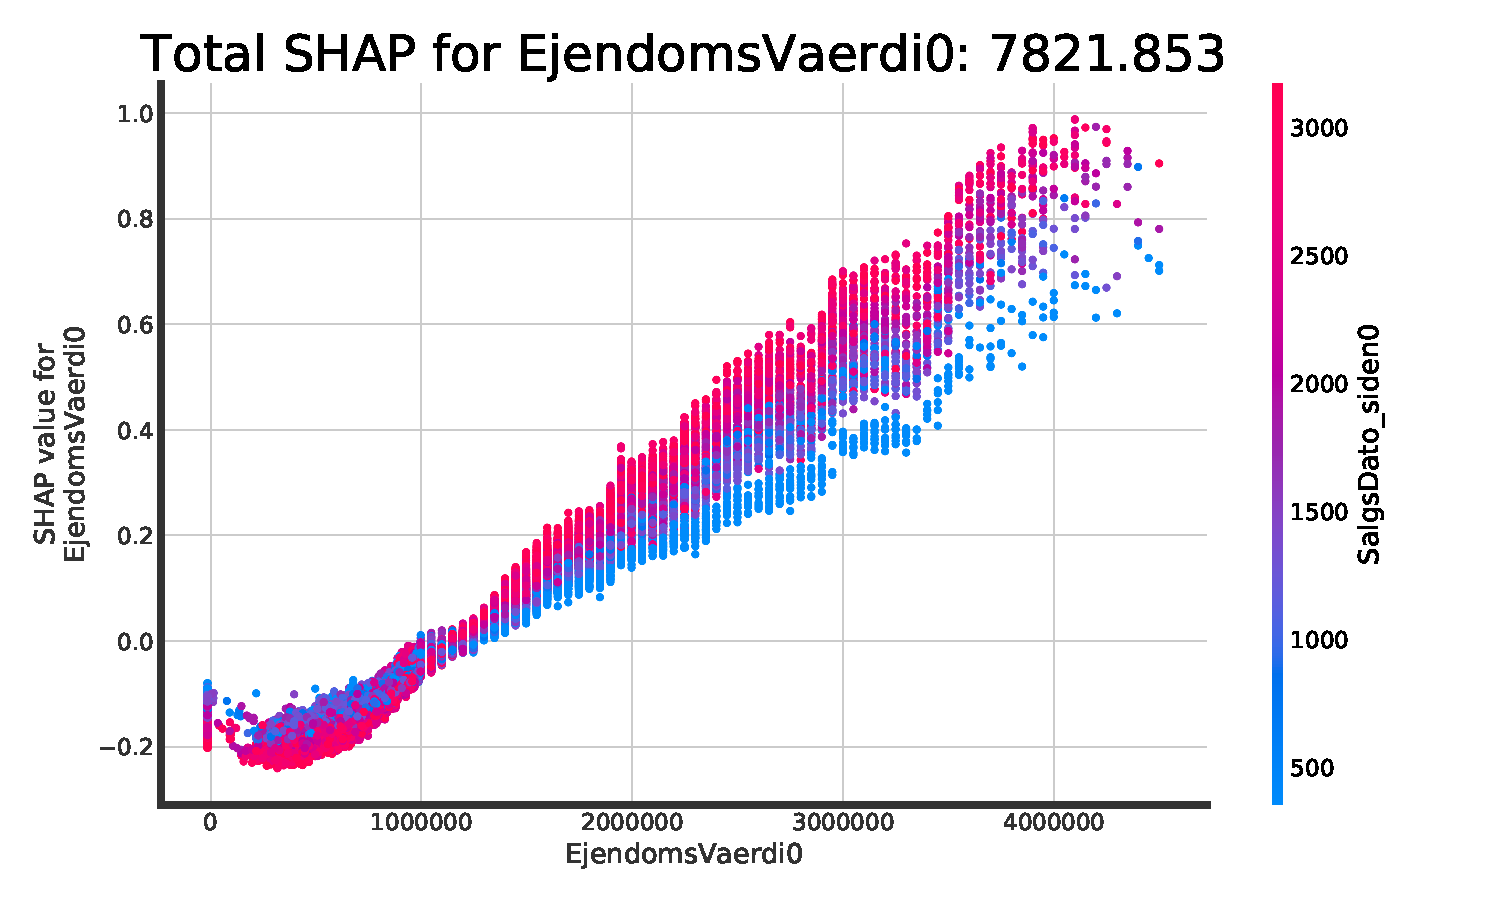
\includegraphics[draft=false, width=0.98\textwidth, trim=15 15 40 40, clip]{figures/housing/Ejerlejlighed_v19_cut_all_Ncols_all_xgb_tight_SHAP_vals_interaction_Vaerdi0.pdf}
  \caption[Feature Importance Interaction Plot for Apartments]
          {Interaction plot of the feature importances for the XGB model on apartments. Here shown for the previous public property valuation (\code{EjendomdsVaerdi0}) colored according to the sales date (\code{SalgsDato_siden0}).} 
  \label{fig:h:shap_overview_interaction}
\end{figure}

What can be concluded from this plot is that apartments with a high PPPV that were sold recently were sold for more than similar apartments (with the same PPPV) which were sold a longer time ago. This is effectively the time dependence of the sales prices. These interaction plots serves as helpful sanity checks to see that the model is actually learning reasonable relationships between the variables. 

\FloatBarrier
\section{Multiple Models}
\label{sec:h:multiple_models}

In addition to the XGBoost model, several other models were also tested. During the project, the LightGBM package \autocite{keLightGBMHighlyEfficient2017} (LGB), was released and started gaining traction in the ML community, especially for large-scale data analysis. LightGBM is also a type of boosted decision tree, however, in comparison to XGBoost, LightGBM implements some extra binning and categorical assumptions that greatly speeds up the fitting process. The LightGBM model was trained in the same way as the XGBoost model with the same hyperparameter optimization process and range for the hyperparameters. 

To compliment the boosted decision trees, a simple linear model (LIN) with $L_2$ loss (ridge regression) was fit. Before it was fit, all of the NANs were median-imputed. This means that all invalid values were replaced with the median for each variable\sidenote[][-6mm]{Since the linear model cannot deal with NANs naturally like XGBoost and LightGBM can.}. All the features were scaled\sidenote[][3mm]{Scaling of input features is generally an important preprocessing step for non-tree based ML models.} with a robust scaler from Scipy \autocite{virtanenSciPyFundamentalAlgorithms2019} in the $(25, 75)$ quantiles range and the regularization parameter was hyperparameter optimized. This linear model is quick and easy to both implement and fit, and can be seen as the simplest baseline model.

The $K$-nearest neighbors (KNN) algorithm was fitted to the data with a data preprocessing pipeline similar to the linear model with median imputation and robust scaling of the input features. The number of neighbors, $K$, was hyperparameter optimized together with the $p$-norm of the metric, $p \in \left\{ 1, 2\right\}$ (Manhattan, Euclidean, see also \autoref{subsec:regularization}).

Finally, support vector machines\sidenote{Known as support vector regression when applied to regression problems \autocite{awadSupportVectorRegression2015}.} (SVR) were used with the same preprocessing pipeline as the previous two methods and hyperparameter optimized for the $L_2$ regularization parameter $C$ and the kernel coefficient $\gamma$ for the radial basis function (RBF) kernel. 

\begin{figure*}[ht!]
  \centerfloat
  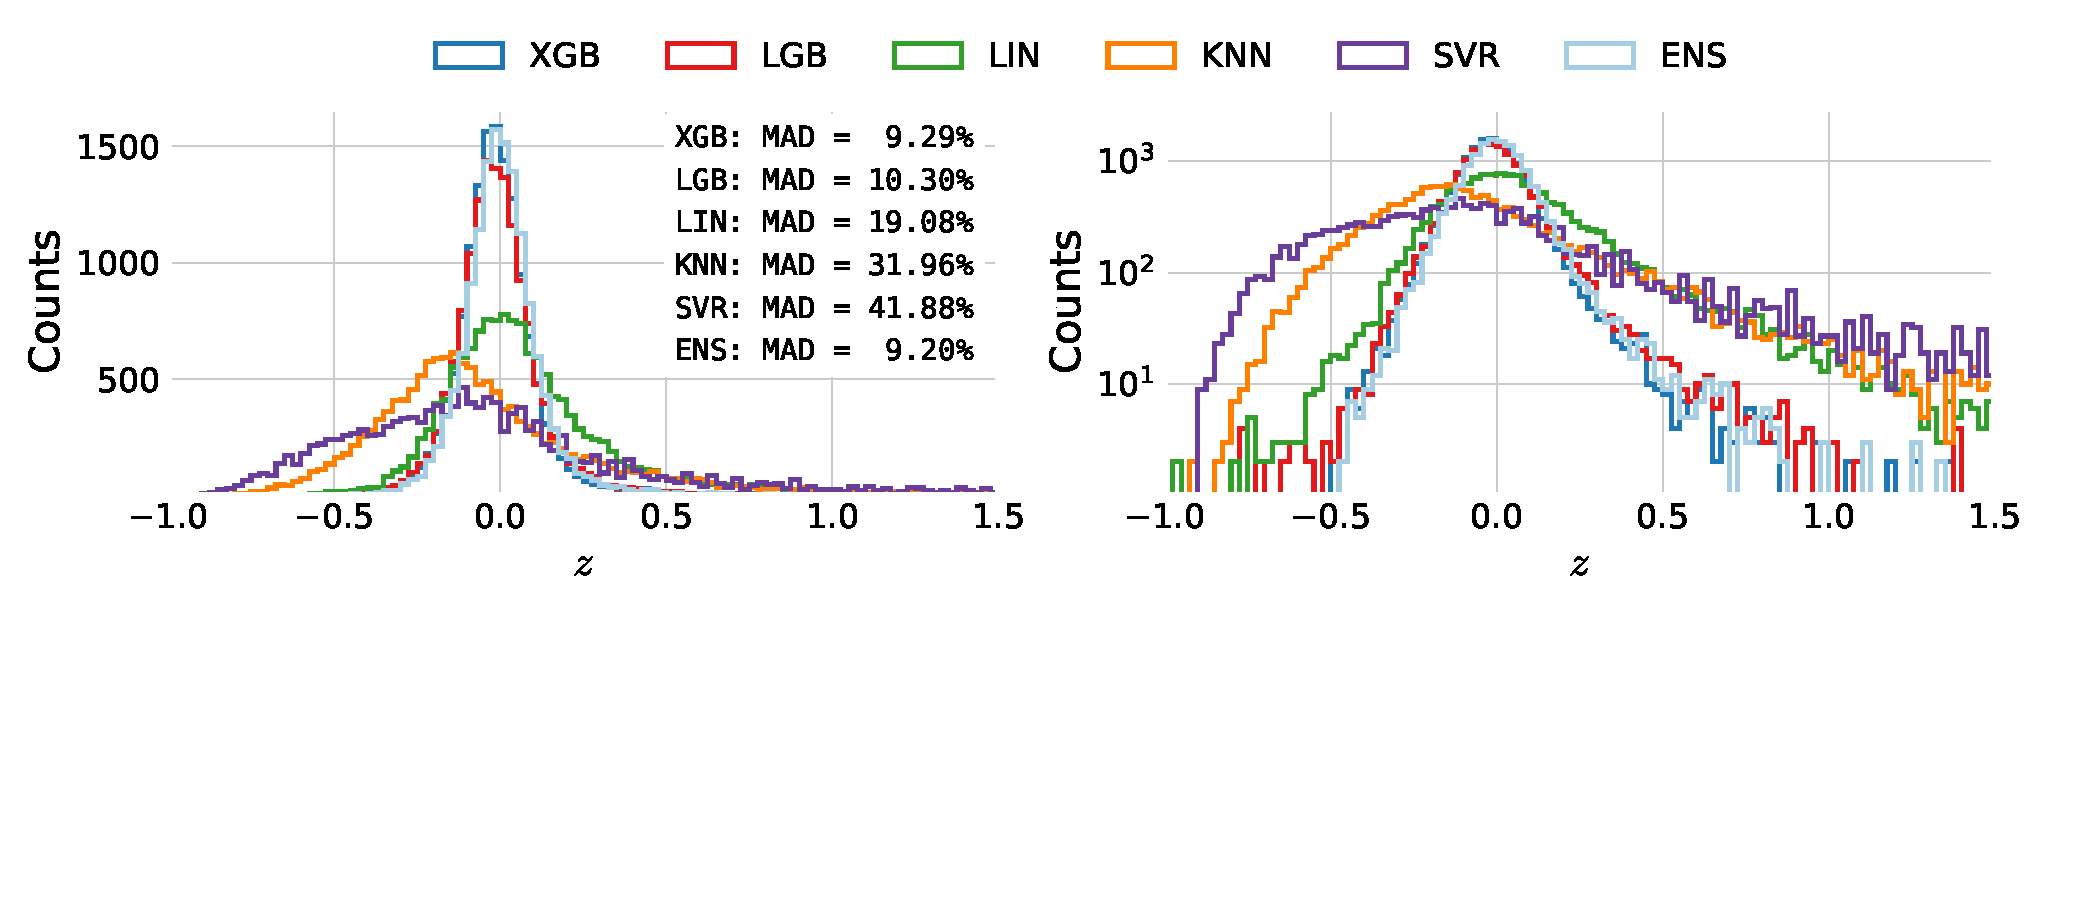
\includegraphics[draft=false, width=0.98\textwidth, trim=10 130 40 10, clip]{figures/housing/Ejerlejlighed_v19_cut_all_Ncols_all_all_models.pdf}
  \caption[Performance Comparison of Multiple Models for Apartments]
          {Distribution of the relative predictions $\vec{z}$ for apartments for the five different models and the ensemble model. The left plot shows the normal histogram (with a linear scale), whereas the right one has a log-scaled $y$-axis to better see the tails of the distributions. The $\mathrm{MAD}_0$ scores for the different models is further shown in the left plot.} 
  \label{fig:h:multiple_models}
\end{figure*}

The results for the five different models are shown in Figure~\ref{fig:h:multiple_models}. The two histograms are the same, the only difference is the logarithmic $y$-axis in the right subplot to better visualize the tails of the distributions. The figure shows how XGBoost and LightGBM are the best-performing models together with the ensemble (\code{ENS}) of the different models. This combined model is explained below. The evaluation score of the test set, \code{MAD}, is also shown on the figure. The scores confirm the visual clue: that the ensemble model performs the best, followed by the XGBoost model.


The five different models -- XGB, LGB, LIN, KNN, SVR -- should be able to each capture different parts of the hyperdimensional phase space and an ensemble of these models would thus be expected to be as good as or better than the best of the individual models. This kind of ensemble model is sometimes called a meta learner or a \emph{super learner} in the statistics community \autocite{vanSuperLearner2007}. 

To make sure that the ensemble model is not just retraining on the training set, and thus end up overfitting, we follow the process from \citet{polleySuperLearnerPrediction2010}. Using cross-validation for time-series\sidenote{See \autoref{subsec:cross_validation}.} data with $10$ folds, the training data is split up into folds sorted by time. Each fold is fitted with all five models, and the prediction of the next fold is made for all five models. This is repeated for the remaining folds until one ends up with a matrix of predictions $\vec{Z} \in \mathbb{R}^{(N \times 5)}$ for $N$ training samples. Since all the folds in $\vec{Z}$ consists of predictions on unseen data\sidenote{The predictions for the very first fold is based on training data.}, this prevents overfitting. The meta learner fits $\vec{Z}$ to the actual predictions of the training data $y$ in the usual way. The combination of a meta learner fitted to the predictions of individual models is called an ensemble model.

At first an XGBoost model was used as the meta learner yielding decent results, however, still performing worse than the single XGB model ($\mathrm{MAD} = \SI{9.57}{\percent}$). To better understand the issue, the meta learner was changed to a linear model which would basically just compute a weighted average of the different models:
\begin{equation}
  \label{eq:h:meta_learner}
  \Psi_\mathrm{meta}(\vec{x}) = \sum_{i=1}^5 \alpha_i \Psi_i(\vec{x}),
\end{equation}
where $\bm{\alpha}$ is a vector of the weights for the meta learner and $\Psi_i$ is one of the individual ML models. The linear model performed even worse than using XGB as the meta learner ($\mathrm{MAD} = \SI{10.48}{\percent}$), yet it was more transparent. During the debugging process it was realized that none of these models actually optimize the evaluation function, $\mathrm{MAD}_0$, directly. The XGBoost model was trained using the Cauchy loss found earlier and the linear regression model using a simple squared error loss. Since a simple weighted average should work as the meta learner \citep{polleySuperLearnerPrediction2010}, a custom algorithm for finding $\bm{\alpha}$ according to $\mathrm{MAD}_0$ was implemented.

Given the training data, the evaluation function as a function of $\bm{\alpha}$ was minimized using the MINUIT algorithm \cite{1975CoPhC..10..343J} via the iminuit \cite{iminuit} Python interface. It yielded decent results, yet they were all very dependent on the initial parameter of the fit indicating many local minima. A scan over the 5-dimensional hyperspace in steps of $0.01$ was thus conducted and the result of this scan was used as the new initial parameter in the minimization routine. This yielded the following result:
\begin{equation}
  \bm{\alpha} = \begin{bmatrix*}[r] \alpha_\mathrm{LIN} \\  \alpha_\mathrm{KNN} \\ \alpha_\mathrm{SVR} \\ \alpha_\mathrm{XGB} \\ \alpha_\mathrm{LGB} \end{bmatrix*} = \begin{bmatrix*}[r] 0.202 \\  0.002 \\ 0.001 \\ 81.302 \\ 20.002 \end{bmatrix*} \times 10^{-2}.
\end{equation}
The fact that it sums to more than \num{1} just corresponds to an overall scaling. When using the found $\bm{\alpha}$ in equation \eqref{eq:h:meta_learner}, one gets the ensemble model (ENS) shown in Figure~\ref{fig:h:multiple_models} with a $\mathrm{MAD} = \SI{9.20}{\percent}$. This value is the evaluation loss on the test set based on only the training data and it outperforms all of the individual models. Even though the ensemble model has the best evaluation score, the performance gain is very little. Since it also requires a lot of training time (five different models have to be fitted), the ensemble model should mostly be seen as a proof of concept.

The paragraphs above refer to apartments, however, the intermediate results for houses showed the same pattern. The combined model along with its performance is shown in Figure~\ref{fig:h:multiple_models_villa}

\section{Discussion}
\label{sec:h:discussion}

The subproject of estimating housing prices has focussed a lot on experimenting with different machine learning models and how to optimize them. As shown in the previous sections, the choice of ML model is by far the most important. Actually, the gain from hyperparameter optimization is quite small, especially considering the amount of time spent on it\sidenote{Not only user-time while programming it, but also the computational ressources spent.}. With the dataset at hand, decent results were achieved, however, they were nowhere near the performance of the realtors' predictions. 

There are two main reasons for this. The first being that realtors are educated within this field and thus have developed the skills required for estimating the price of a house during many years of hard work. The second reason is the fact that the realtors have access to a lot more information than the ML models have. The ML models seen so far have not been trained on any \emph{indoor variables}. The area of the house, the number of rooms, the name of the street, and the distance to a highway are all variables that are in the data set but none of them describe the overall quality of the house, the maintenance level, the age of the kitchen or bathroom. These indoor features are invisible to the ML model. 

During the project it was investigated how to get access to these variables. At first the online images from each sale were suggested. Unfortunately, it turned out that Boligsiden only have the right to use them while a residence is for sale; when it is sold all rights return to the photographer. Fortunately, the images are not the only piece of data that provide more information about the condition of the residence: also the descriptions do that. 

The descriptions turned out to be available for most of the sales and were investigated for a short period. At that time of the small investigation, the $\mathrm{MAD}_0$ for (a subset of) the apartments was around $\pm \SI{14}{\percent}$ and $\pm \SI{20}{\percent}$ for houses. By using methods from the big natural language processing (NLP) community within the field of machine learning, it was possible to reduce the $\mathrm{MAD}_0$ to around $\pm \SI{12}{\percent}$ and $\pm \SI{15}{\percent}$ for apartments and houses respectively. From the improvement in performance it is noticeable how apartments in general are much more uniform compared to houses where the \q{inside} is more decisive regarding the price. 

\begin{figure}[h!]
  \centering
  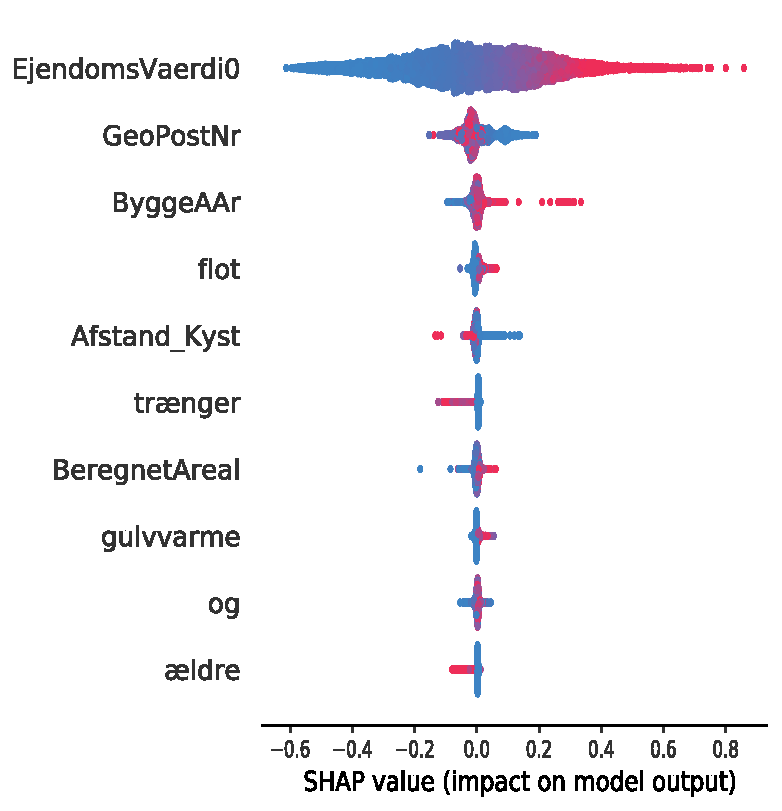
\includegraphics[width=0.8\textwidth]{figures/housing_text/villa_tfidf.pdf}
  \caption[Feature Importance of Villas With Descriptions]
          {Feature importance of villas when the descriptions are also used. The variables are sorted top to bottom according to their overall feature importance, i.e. the previous public property valuation \code{EjendomdsVaerdi0} is the most important single feature. Along the $x$-axis is the impact on model output, in this example the price in \si{\Mkr} This axis is colored by the value of the feature, from \textcolor{blue}{low} (blue) to \textcolor{red}{high} (red). In this particular example we see that high values of the previous public property valuation has high, positive impact on the model prediction -- exactly as expected. This is in contrast to the word \q{requires} (\colorbox{light-gray}{\texttt{trænger}}) where a high value has a negative impact.} 
  \label{fig:h:shap_text}
\end{figure}

The methods for translating the text to numerical variables decipherable by classical ML models were for instance simple \emph{bag of words} (BOW) models and \emph{Term Frequency, Inverse Document Frequency} (TF-IDF) but also slightly more advanced statistical tools such as \emph{Latent Dirichlet Allocation} (LDA). 

An old example of this was a house based model that was trained with the five numerical variables\sidenote{With the Danish names: \code{Ejendomsvaerdi0}, \code{GeoPostNr}, \code{ByggeAAr}, \code{Afstand_Kyst}, and \code{BeregnetAreal}.}: the PPPV, postal code, year of construction, distance to shore, and the weighted area. In addition ti the numerical variables, also the text descriptions (encoded with TF-IDF) were trained on. Figure~\ref{fig:h:shap_text} shows the SHAP summary plot of the trained model. The three most important features turned out to be the numerical ones, however, the word \code{flot} (\q{pretty}) was ranked \nth{4}. The model also learnt that \code{flot} has a positive impact on the price compared to \colorbox{light-gray}{\texttt{trænger}} (\q{requires}) which has a negative impact.
% \code{Ejendomsvaerdi0} (PPPV), \code{GeoPostNr} (postal code), \code{ByggeAAr} (year of construction), \code{Afstand_Kyst} (distance to shore), and \code{BeregnetAreal} (weighted area) 

The descriptions turned out to be more time-consuming to extract for Boligsiden and along with the fact that the overall deadline was quickly approaching, the remaining time was focussed on the main part of the project, the quark gluon discrimination. Given more time, the text analysis would definitely be the first step for further improving the accuracy and precision of the price predictions. 

Another step would be to apply more modern deep learning\sidenote{Basically advanced neural networks with many layers.} methods. These methods were briefly experimented with in the initial stages of this subproject but showed inferior performance compared to boosted decision trees. It is generally accepted in the ML community (with some modifications) that neural networks underperform, or at least not outperform, classic ML methods on structured data\sidenote{Structured data are data that can be described by a spread sheet, i.e. has a well-defined number of variables and observations. This is why it is also known as \emph{tabular data}.} \autocite{klambauerSelfNormalizingNeuralNetworks2017}. Most often they have the inherent complexity needed to perform as well as other ML methods, however, this requires extensive architecture optimization, or, in short; the hypothesis space for neural networks is much larger than classical ML methods and thus requires more care to avoid overfitting.

\section{Conclusion}
\label{sec:h:conclusion}

Estimating housing prices is not easy and computer models are still not as high performing as professional realtors, however, the field of automated housing predictions is rapidly progressing. In this first half of the thesis, Danish housing prices were predicting using a multitude of different machine learning models and techniques. A fitting pipeline consisting of first optimizing for the best loss function, sample weight, and transformation of the data was tested followed by a comparison of the random search and Bayesian optimization hyperparameter optimization routines. This pipeline was evaluated for the XGBoost model and its forecasting abilities measured along with an inspection of the most important features according to this model. This showed that the previous public property valuations are still the highest ranking features followed by the area, however, the data augmented price index turned out to be in the top five as well. This shows that feature engineering is still an important technique in machine learning. 

The model's performance, as measured by the median absolute deviation around zero, $\mathrm{MAD}_0$, on the (unseen) test set (all sales in \num{2018}) is found to be \SI{9.3}{\percent} for apartments and \SI{15.8}{\percent} for houses. For a subset af the sales (around \SI{60}{\percent}), which is still a pretty loose selection, the scores were improved even further down to \SI{8.5}{\percent} and \SI{14.9}{\percent}. These numbers should be compared to the performance of the realtors which were \SI{4.9}{\percent} and \SI{7.6}{\percent}. The apartment model correctly predict more than \SI{41}{\percent} of the price of apartments to be within $\pm \SI{5}{\percent}$, around \SI{70}{\percent} within $\pm \SI{10}{\percent}$, and more than \SI{91}{\percent} within $\pm \SI{20}{\percent}$. 

The results show that houses are much harder to predict than apartments since they are much more diverse. A short study into using the text descriptions of the sales showed that the model for houses could potentially improve with up to \num{5} percentage points, while only a around \num{2} percentage points for apartments. Another way of improving the model was by using an ensemble of different models, which also showed improvements, however small, and was not concluded to be worth the extra time compared to a single model.

%  # # # # # # # # # # # # # # # # # # # # # # # # # # # # # # # # # # # # # # # # # # # # # # # # # # # # # # # # # # # # # # # # # # # # # # # # # # # # # # # # # # # # # # # # # # # # # # # # # # # # # # # # # # # # # # # # # # # # # # # # # # # # # # # # # # # # # # # # # # # # # # # # # # # # # # # # # # # 

\phantomsection
\chapter*{}
\addcontentsline{toc}{part}{Part II}
\label{part2}
{\Huge \rmfamily Part II}
% \cleardoublepage

% \part{Part II}
% \part{Particle Physics and Quark Gluon Discrimination}
% \label{part2}

% \part*{Part2}
% \label{part2}
% \phantomsection
% \addcontentsline{toc}{part}{Part II}
% Part \RNum{2} of this thesis deals with particle physics and the discriminatory power of machine learning for quark-gluon identification and subsequent analysis. In \autoref{ch:hep:particle_physcis_LEP} the theory of the Standard Model is introduced together with a description of the ALEPH detector. Theory is applied in \autoref{ch:quark_gluon_analysis} where the types of jets and events in each collision is analysed using machine learning to improve the understanding of how gluon jets hadronizes and splits: simply said how they look and behave. 


\FloatBarrier
\chapter{Particle Physics and LEP}
\label{ch:hep:particle_physcis_LEP}
\epigraph{\textit{``Not only is the Universe stranger than we think, it is stranger than we can think.''}}{--- Werner Heisenberg}

The aim of this chapter is to introduce the reader to the level of particle physics required for understanding the following chapter, in particular introducing the Standard Model in \autoref{sec:hep:standard_model}, the theory behind quark hadronization in \autoref{sec:hep:quark_hadronization}, and the ALEPH detector at LEP in \autoref{sec:hep:aleph}. The goal is not to make a deep and thorough introduction to the field as this is not needed for the following analysis  along with the fact that the author is no particle physicist himself. 


\FloatBarrier
\section{The Standard Model}
\label{sec:hep:standard_model}

The \emph{Standard Model} (SM) \autocite{glashowPartialsymmetriesWeakInteractions1961,salamWeakElectromagneticInteractions1994,weinbergModelLeptons1967} of particle physics is currently the best known description of the elementary particles and thus describes the fundamental building blocks of our Universe. An overview of the particles explained by the Standard Model is shown in the typical tabular form seen in Figure~\ref{fig:hep:standard_model}. In general, particles comes in two categories: \emph{bosons} and \emph{fermions}. 

\begin{figure*}
  \centerfloat
  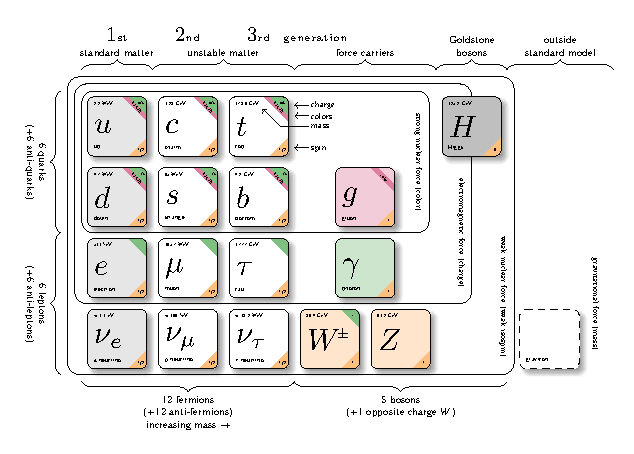
\includegraphics[width=0.99\textwidth]{figures/standard_model/sm.pdf}
  \caption[The Standard Model]{The Standard Model. Inspired by \citet{purcellGoParticleQuest2012} using the template by \citet{burgardStandardModelPhysics} with manually updated masses according to \citet{particledatagroupReviewParticlePhysics2018}.}
  \label{fig:hep:standard_model}
\end{figure*}

The fermions, the left part of the figure, are particles with half-integer spin that obey Fermi-Dirac statistics and are further subdivided into \emph{quarks} (upper left in figure) and \emph{leptons} (lower left). The quarks interact with all of the four known forces\sidenote{Gravity, electromagnetism, and the strong and weak force.}, including the strong force. In contrary the leptons do not interact with the strong force. Quarks are never observed freely but are always combined into \emph{hadrons} due to \emph{color confinement} which is further explained in \autoref{sec:hep:quark_hadronization}. An example of this are protons which consists of two up-quarks and a down-quark. Leptons exist as either the charged leptons\sidenote{The electron $e$, the muon $\mu$, and the tau $\tau$.} or as neutral leptons, the so-called neutrinos\sidenote{The electron neutrine $\nu_e$, the muon neutrino $\nu_\mu$, and the tau neutrino $\nu_\tau$.}. The fermions come in three generations with increasing mass.

The bosons, the right part of the figure, are the force-carrying particles (with integer spin and which obey Bose-Einstein statistics) where the gluon, $g$, mediates the strong nuclear force (color charge), the photon, $\gamma$, mediates the electromagnetic force (charge), and the two $W^\pm$ and the $Z$ bosons mediate the weak nuclear force (weak isospin). The Higgs boson $H$, experimentally discovered in 2012 \autocite{theatlascollaborationObservationNewParticle2012,thecmscollaborationObservationNewBoson2012}, does not mediate any forces but interacts with all massive particles and explains why particles have mass. 

All particles have antiparticles which are particles with opposite charge but the same mass. Some particles are their own antiparticles\sidenote[][4mm]{The photon, the $Z$, and the Higgs.}, such as the $Z$. At the Large Electron Positron collider (LEP), see \autoref{sec:hep:aleph}, electrons $e^-$ and their antiparticles positrons $e^+$ were collided at an energy of around \SI{91}{\GeV}. This particular energy was chosen since this is at the resonance peak of the $Z$. Its mass distribution follows a Cauchy distribution (also known as Breit-Wigner) with mean\sidenote{Calculated in natural units where $c=\hbar=1$ which will also be used throughout this thesis.} $m_Z = \SI{91.1876 \pm 0.0021}{\GeV}$ and a full width of $\Gamma_Z = \SI{2.4952 \pm 0.0023}{\GeV}$. LEP was as such a $Z$-factory. The $Z$, however, is only very short-lived with a half-life of $1/ \Gamma_Z \sim \SI{2.6e-25}{s}$. The decay mode for this unstable $Z$ particle is primarily to hadrons (\SI{69.91\pm 0.06}{\percent}) where the ratio (R) for $b$-quarks is $R_b = \left( Z \rightarrow b\bar{b} \right) = \SI{15.12 \pm 0.05}{\percent}$ and $R_g = \left( Z \rightarrow ggg \right) < \SI{1.1 \pm 0.05}{\percent}$ for gluons \autocite{particledatagroupReviewParticlePhysics2018}. The fact that the $Z$ is neutral and its own anti-particle means that it generally decays to a particle--anti-particle pair (due to charge-conservation). Antiparticles are written with a bar on top, e.g. the $\bar{b}$-quark is the antiparticle of the $b$-quark.

 

\FloatBarrier
\section{Quark Hadronization}
\label{sec:hep:quark_hadronization}

The electron-positron $e^+ e^-$ annihilations at LEP are complicated events that require advanced high-energy particle physics theory to be properly understood. Most of the aspects of the process is well-described by now, however, especially the hadronization process is still an area of active research. To better get an overview of the different stages of the $e^+e^-$ annihilations, see the Feynman diagram in Figure~\ref{fig:hep:feynman_3j_qqg}. 

\begin{marginfigure}
  \centerfloat
  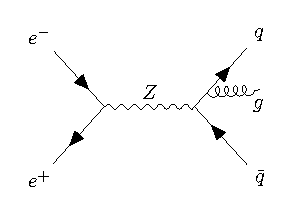
\includegraphics[width=0.99\textwidth, trim=10 10 10 10, clip]{figures/feynman_diagrams/eeZqqg.pdf}
  \caption[Feynman Diagram for the Jet Production at LEP]{Feynman diagram showing the $e^+ e^- \rightarrow Z^0$ production at LEP. The $Z$ has several decay modes where the $Z \rightarrow q\bar{q}g$ is shown here.}
  \label{fig:hep:feynman_3j_qqg}
\end{marginfigure}

Reading from left to right, the electron and the positron annihilates to a $Z$. This interaction is well-described by quantum electrodynamics (QED), a theory that has been around for more than 60 years by now. As mentioned in the previous section, the $Z$ has several decays modes, yet most of these are background processes of no interest in this project and the focus for now will be the decay mode $Z \rightarrow q\bar{q}$ ($Z$ to quark--anti-quark) as seen in the Feynman diagram. The particles produced by the $Z$-decay are called primary \emph{partons}. Since this process involves quarks, and thus color charge, QED is no longer an adequate theory: quantum chromodynamics (QCD) is needed \autocite{Armstrong1998hy}. The $q\bar{q}$ pair in this example acts as (color) dipoles from which a gluon can radiate. It can be shown with QCD that the gluon can only be radiated inside the cone that the $q\bar{q}$ pair spans \autocite{bierlichRopeHadronizationGeometry2016}. As mentioned in the introduction, quarks cannot exist freely (due to \emph{confinement}) and we therefore cannot observe the individual partons in the $q\bar{q}g$ event illustrated in the Feynman diagram. Confinement is basically the QCD principle saying that quarks are always confined, or bound, inside hadrons. The initial partons (carrying color charge) are converted to (color-neutral) hadrons by non-perturbative QCD processes in what is called \emph{hadronization}, and these hadrons can be measured. 

\begin{marginfigure}
  \centerfloat
  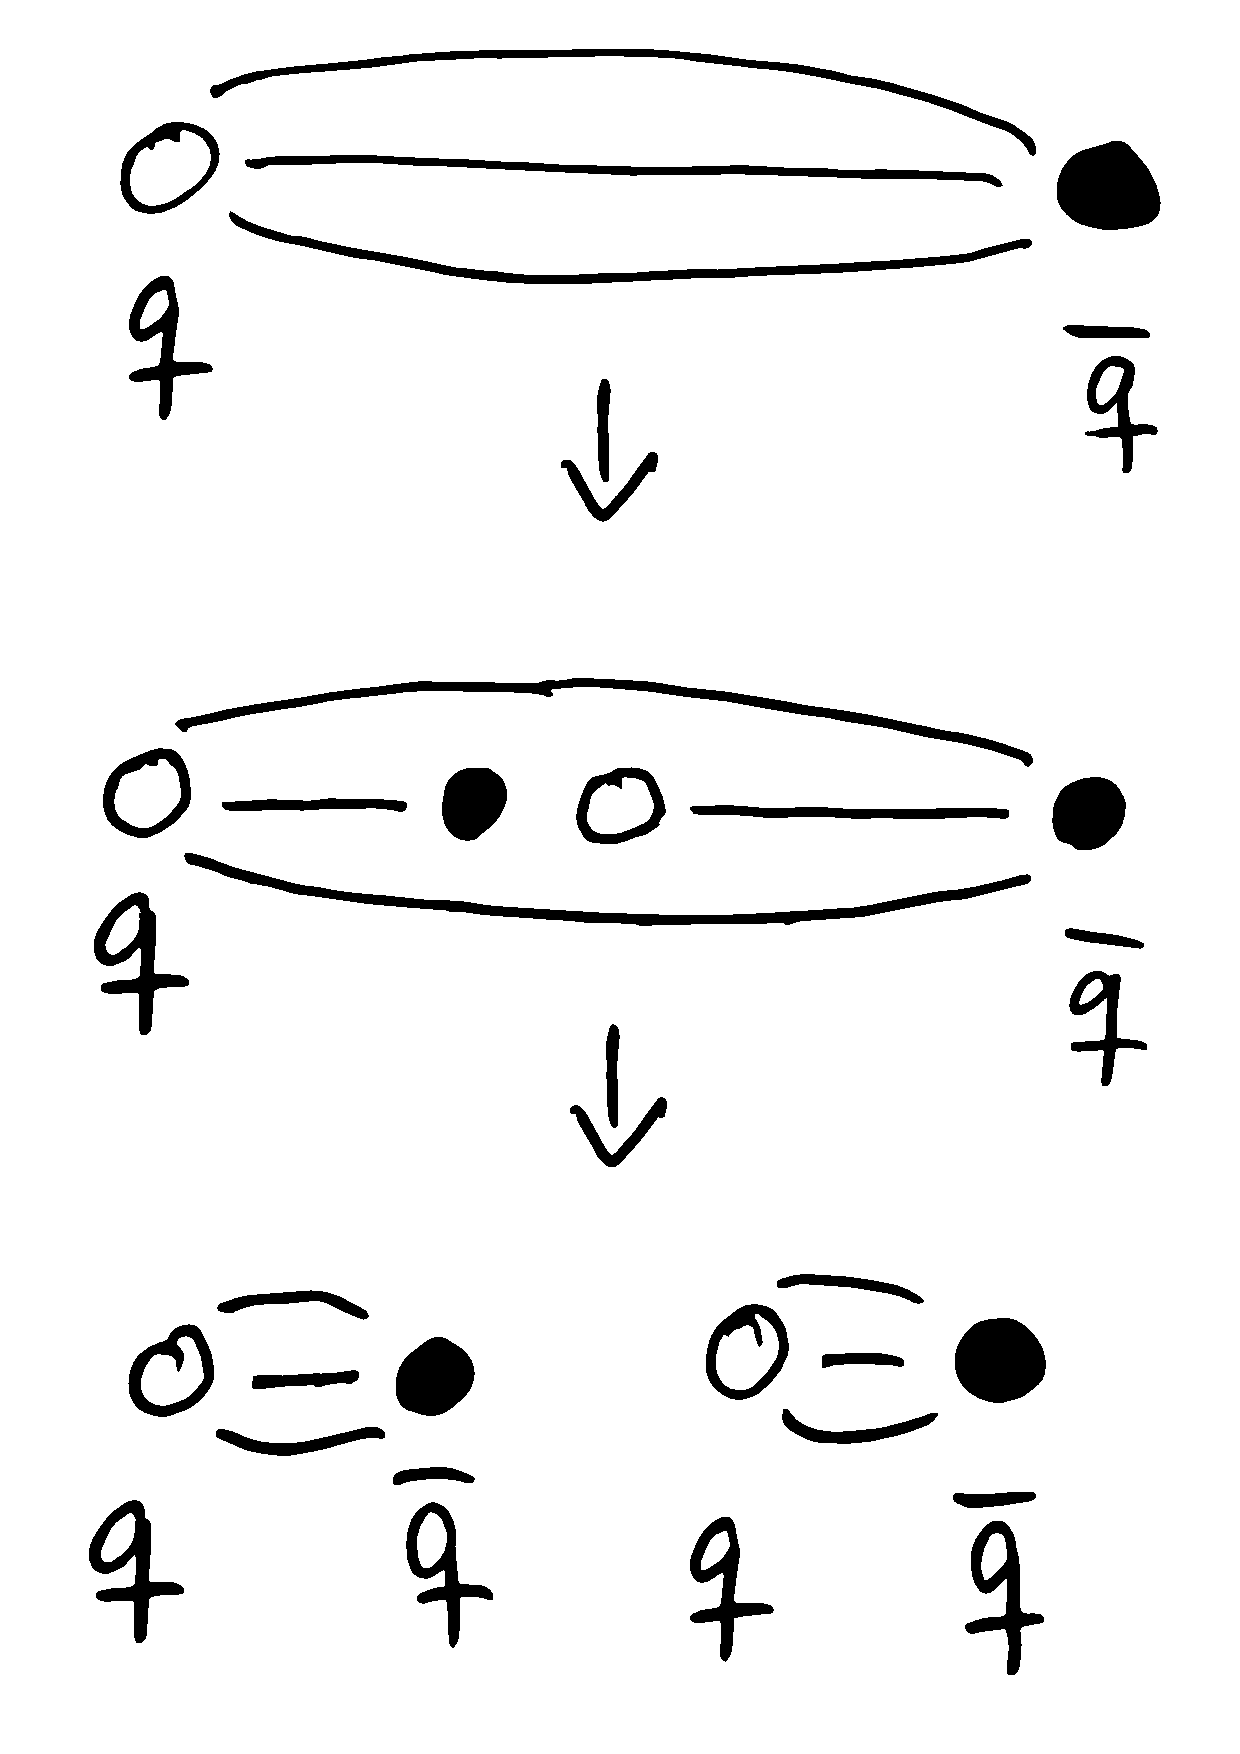
\includegraphics[width=0.99\textwidth]{figures/quark_splitting/quark_splitting.pdf}
  \caption[Quark Splitting]{Illustration of the quarks splitting as explained by the Lund string model. For large charge separation the (color) field lines seem to be compressed to a tube-like region, where the strong interactions are mediated by the massless gluons (that couple to the color charge of quarks). When the two quarks are separated enough, the potential energy is released by the production of a new $q\bar{q}$ pair.}
  \label{fig:hep:quark_splitting_strings}
\end{marginfigure}

The hadronization process is not yet fully modelled and currently two competing models for predicting the hadronization pattern exists: the Lund string model and the cluster model. In this project only the former of the models will be used. The Lund string model \autocite{anderssonPartonFragmentationString1983} is the theoretical framework underlying the widely used Monte Carlo event generator PYTHIA \autocite{sjostrandIntroductionPYTHIA2015}. The string model is based on the observation that (color) field lines between quarks seem to compress into a tube-like region mediated by gluons, see the top part of Figure~\ref{fig:hep:quark_splitting_strings}. The field can be described by a linearly rising potential $V(r)=\kappa r$ at large distances\sidenote[][4mm]{At small distances a Coulumb term has to be included, however, this term is assumed to be negligible by the Lund string model.}, where $r$ is the distance and $\kappa$ is the strength of the potential \autocite{buckleyGeneralpurposeEventGenerators2011}. This field is similar to the (constant) force of a string: $V(r)=\kappa r \Rightarrow F(r) = -\kappa$ where $\kappa$ is to be regarded as the spring tension. As quarks move apart, the potential energy stored in the \q{string} increases until it is large enough to \q{snap} and convert its potential energy into mass. This mass energy is released with the production of a new $q\bar{q}$ pair as this is energetically favorable, see the rest of Figure~\ref{fig:hep:quark_splitting_strings}. 
% The gluons can thus be seen as kinks on a string carrying energy-momentum.

An example of the hadronization process, or the transition from initial partons to final hadrons is sketched in Figure~\ref{fig:hep:hadronization}. Here the production of two kaons ($\mathrm{K}^-$ and $\mathrm{K}^+$) and two pions ($\pi^-$ and $\pi^0$) are shown. Since particles are created by \q{splits} in the \q{string}, and the fact that there is energy-momentum conservation, they all have to share the total energy stored in the string. This is described by the fragmentation function:
\begin{equation}
  f(z) \propto \frac{(1-z)^a}{z} \exp \left(- \frac{b m^2}{z} \right),
\end{equation}
where $0 \leq z \leq 1$ is the remaining momentum that the new hadron takes, $a$ and $b$ are constants, and $m$ is the mass\sidenote{Where $m \rightarrow m_\perp$ for particles with transverse momentum.} \autocite{bierlichRopeHadronizationGeometry2016}. When the system runs out of available momentum, it will stop producing new hadrons and the fragmentation function thus explains the distribution of the final state particles. The Lund string model can be extended from only $q\bar{q}$ events to $q\bar{q}g$ events where it predicts that the cones spanning the angular regions $qg$ and $\bar{q}g$ should receive enhanced particle production compared to the $q\bar{q}$ region. This prediction by the Lund string model is also measured in $e^+e^-$ collisions \autocite{buckleyGeneralpurposeEventGenerators2011}.

\begin{figure}
  \centerfloat
  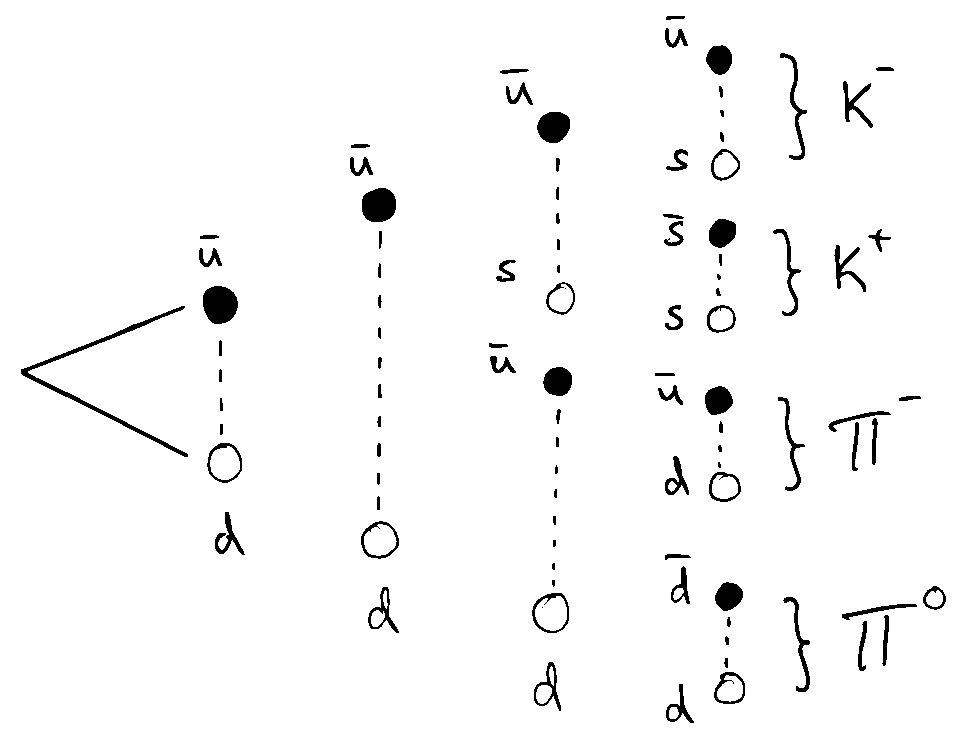
\includegraphics[width=0.9\textwidth]{figures/hadronization/hadronization.pdf}
  \caption[Hadronization Process]{Illustration of the hadronization process by which $\bar{u}$- and $d$-quarks decay into four different mesons. The theoretical strings are shown as dashed lines and particles as circles, where filled circles are antiparticles.}
  \label{fig:hep:hadronization}
\end{figure}

The initial partons produced as $Z$ decay therefore decay to final state hadrons\sidenote{To either mesons which consist of two quarks (color--anti-color) or baryons (\mbox{r-g-b}) which consist of three quarks.} which create a whole \q{shower} in the direction of the initial parton: this is called a \emph{parton shower} and it is this parton shower observed as particles, a \emph{jet}, that is measured in the detector. The reverse computation from tracks measured in the detector is done with the use of \emph{jet clustering} algorithms. The detector and the clustering algorithms are described in the following section.


\FloatBarrier
\section{The ALEPH Detector and LEP}
\label{sec:hep:aleph}

The Large Electron Positron collider (LEP) was a particle collider at CERN in Switzerland operating from \num{1989} to \num{2000}. It collided counter-rotating bunches of electrons and positrons in a giant ring with a circumference of more than \SI{26}{\km}. The first phase, LEP1, ran from \num{1989} to \num{1995} at the $Z$ resonance $\SI{91}{\GeV}$ and the second phase, LEP2, continued afterwards with energies closer to $\SI{200}{\GeV}$ for $W^+W^-$ pair production \autocite{Armstrong1998hy}, however, it is only the data collected at the energy around $\sqrt{s} = \SI{91.3}{\GeV}$ (called the \emph{$Z$ peak data}) that is used throughout the rest of this project. There were four independent detectors at the LEP experiment, one of them ALEPH\sidenote{Together with DELPHI, L3, and OPAL.}.

\begin{figure}
  \centerfloat
  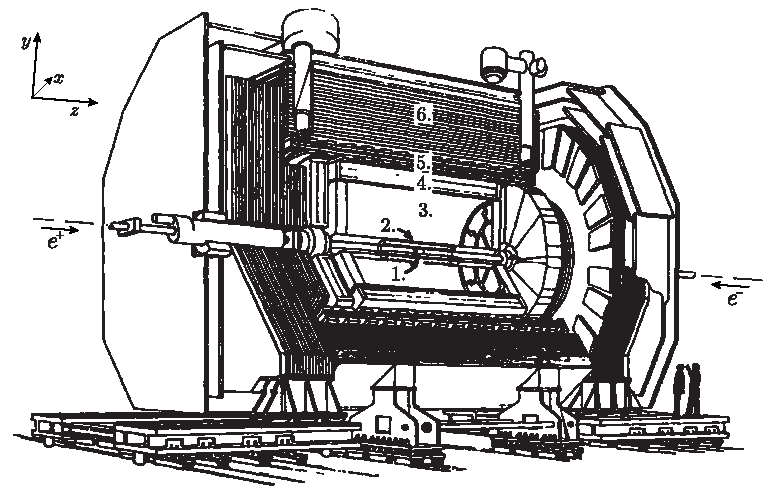
\includegraphics[width=0.99\textwidth]{figures/ALEPH/aleph.pdf}
  \caption[The ALEPH Detector]{The ALEPH detector at LEP. 1) Vertex detector (VDET). 2) Drift chamber (ITC). 3) Time projection chamber (TPC). 4) Electromagnetic calorimeter (ECAL). 5) Superconducting magnet coil. 6) Hadron calorimeter (HCAL). Adapted from \citet{buskulicInvestigationBd0Bs01994}.}
  \label{fig:hep:aleph_detector}
\end{figure}

The \emph{apparatus for LEP physics} (ALEPH) was a particle detector at LEP with a wide coverage, almost $4 \pi$, consisting of cylindrical subdetectors, see Figure~\ref{fig:hep:aleph_detector}, with the coordinate system shown in the upper left corner\sidenote{The $z$-axis pointing along the beam direction, the $y$-axis pointing upwards, and the $x$-axis pointing towards the center of LEP.}. The polar angle $\theta$ is illustrated in Figure~\ref{fig:hep:aleph_detector_theta} together with the transverse (longitudinal) momentum $p_\perp$ ($p_L$) and the azimuthal angle $\phi$ in Figure~\ref{fig:hep:aleph_detector_phi}. The ALEPH detector was designed to measure the energy deposited in the calorimeters by charged and neutral particles, measure the momenta of charged particles, measure the distance of travel of short-lived particles, and to identify the three lepton flavors (electron, muon, tau) \autocite{buskulicInvestigationBd0Bs01994}. As can be seen in Figure~\ref{fig:hep:aleph_detector}, ALEPH consisted of five subdetectors (the vertex detector (VDET), the drift chamber (ITC), and the time projection chamber (TPC)) and two calorimeters (the electromagnetic (ECAL) and the hadronic calorimeters (HCAL)). 

\begin{marginfigure}[-3cm]
  \centerfloat
  \includegraphics[width=0.9\textwidth]{figures/yz_coordinate_system/yz_coords.pdf}
  \caption[Polar Angle]{The polar angle $\theta$ defined in the $zy$ coordinate system}
  \label{fig:hep:aleph_detector_theta}
\end{marginfigure}
\begin{marginfigure}
  \centerfloat
  \includegraphics[width=0.9\textwidth]{figures/xy_coordinate_system/xy_coords.pdf}
  \caption[Azimuthal Angle]{The azimuthal angle $\phi$ defined in the $xy$ coordinate system. }
  \label{fig:hep:aleph_detector_phi}
\end{marginfigure}

The three innermost detectors allow for precise tracking of the charged particles produced in the parton shower and the two outer calorimeters of precise energy measurements for both charged and neutral particles going through the detector. The calorimeters measure the energy of particles by absorbing them. 

When a particle interacts with the detector, a small electric charge is measured, referred to as hits. A hadronic event from a parton shower may leave a score of charged tracks resulting in hundreds of hits in the detectors (VDET, ITC, and TPC) which are fitted\sidenote[][4mm]{The process of fitting tracks is called \emph{track reconstruction} in high energy particle physics.} with Kalman filters \autocite{kalmanNewApproachLinear1960} to obtain global track fits, of which bad charged tracks are discarded for further analysis. The tracks are helical due to the presence of a \SI{1.5}{T} magnetic field which curves the charged particles according to their transverse momentum.

The energy resolution $\sigma$ of the calorimeters, or the \emph{calorimeter performance}, is expected to increase with $\sqrt{E}$. In fact, it was found at ALEPH that the energy dependence of the resolution follows the parametrization \autocite{buskulicInvestigationBd0Bs01994}:
\begin{equation}
  \label{eq:hep:ALEPH_energy_resolution}
  \sigma(E) = \left( \left( 0.59 \pm 0.03 \right) \cdot \sqrt{E / \mathrm{GeV}} +  \left(0.6 \pm 0.3 \right) \right) \mathrm{GeV}.
\end{equation}
Even though $\sigma(E)$ increases with $E$, the relative resolutions improves with higher energies. Since Nature is never measured directly, the results obtained in a measurement are thus products of both model and experimental uncertainties folded together. To unfold the measurements to obtain experiment-independent results, the uncertainties are important to understand. Of course there are dozens of other uncertainties in an advanced experiment like ALEPH, however, the energy dependence is the primary focus in this project. 

\section{Jet Clustering}
\label{sec:hep:jet_clustering}

Since the initial partons created as decay products from the $Z$ are unstable themselves, what is measured in the detector is a whole shower of hadrons seen as charged tracks in the detectors and energy deposits in the calorimeters. However, say that the $Z$  decayed to a $b\bar{b}$ event. In this case the two $b$'s would be back-to-back and the final hadrons would be observed approximately in the same direction as the $b$'s were created. The interest of the experiment is not to measure the final hadrons, but rather to infer information about the initial quarks and gluons. This is done via the reverse-engineering process called \emph{jet clustering}. Over the years many clustering algorithms have been developed, however, most of these are younger than LEP. In the ALEPH experiment the JADE algorithm was used \autocite{bartelExperimentalStudyJets1981}. JADE is a sequential recombination algorithm where final state particles are initially described as individual so-called pseudo-jets which are then recursively merged to larger jets according to their inter-jet distance $d^2_{ij}$. The distance measure for JADE is:
\begin{equation}
  d^2_{ij} = \frac{2E_i E_j (1 - \cos\theta_{ij})}{E^2_\mathrm{vis}},
\end{equation}
where $E_\mathrm{vis}$ is the visible energy\sidenote{The total sum of energies in the event.} and $\theta_{ij}$ is the angle between jet $i$ and $j$. The JADE algorithm computes $d^2_{ij}$ for all combinations of jets and merges the two jets with the lowest $d^2_{ij}$, continuing like that recursively until $\min(d^2_{ij}) > d^2_\mathrm{cut}$ for some predefined value of $d^2_\mathrm{cut}$. 
% In the dataset at hand, only the final jets were available and not the jet constituents, unfortunately. 

\section{The Variables}
The overall goal of the project is to be able to discriminate quarks and gluons using only vertex variables. The reason for the last condition is that the goal is to better understand the shape distributions of gluons in which there is still significant differences between Monte Carlo (MC) simulations and Data. Therefore only vertex variables will be used to avoid any biases introduced by using shape-related variables to detect differences in shape-distributions. 
The vertex variables are a subset of all variables which include the three variables \code{projet}, \code{bqvjet}, and \code{ptlrel}. These three particular variables have each shown discriminatory power in separating $b$-quarks from light quarks and gluons. 

% \begin{enumerate}
\begin{enumerate}[leftmargin=*,labelindent=16pt]
  
  \item[\hspace{0.5cm} \code{projet}:] \newthought{Probability of significant lifetime}. For each track in the jet, the impact parameter $\delta$ is computed. This parameter is the minimum distance between the estimated $Z$ decay point and the track itself and its sign depends on whether or not the point of closest approach is in front of or behind the $Z$ decay point (relative to the momentum). From $\delta$, the significance $\mathcal{S}$ -- which is $\delta / \sigma_\delta$ -- is computed and is thus a measure of the certainty of a measured track being from the primary vertex. High values of $\mathcal{S}$ is typically an indicator of $b$ jets, since long-lived particles typically decay in front of the $Z$ relative to the jet direction, while $uds$-jets generally have small significance and might as well have negative values of $\mathcal{S}$. An illustration of the difference in significance between $uds$-jets and $b$-jets can be seen in Figure~\ref{fig:hep:significance}.
  \begin{marginfigure}[-0.5cm]
    \centerfloat
    \includegraphics[width=0.9\textwidth]{figures/projet_significance/projet_significance.pdf}
    \caption[Track Significance]{Distribution showing the difference in significance $\mathcal{S}$ between $uds$-jets and $b$-jets. Based on own, simulated data to illustrate this difference.}
    \label{fig:hep:significance}
  \end{marginfigure} 
  \noindent From $\mathcal{S}$, the track probability $\mathcal{P}_\mathrm{track}$ of a track originating at the decay point of the $Z$ can be computed, which can further be aggregated across all tracks within a jet to form the jet probability $\mathcal{P}_\mathrm{jet}$ which \code{projet} is a function of \autocite{buskulicPreciseMeasurementGZ1993}. 
  Whether or not $\mathcal{P}_\mathrm{jet}$ is strictly a probability can be discussed but it is related to the probability of all tracks within a jet to originate from long-lived particles, which itself is a good indicator of the jet being a $b$- (or $c$-) jet. This variable further has the advantage of being independent of any vertex algorithm.


  \item[\hspace{0.5cm} \code{bqvjet}:] \newthought{$b$-quark vertex of jet}. For any jet with well measured\sidenote{Meaning that there are at least four TPC hits and the fit has a reduced $\chi^2$ of less than four \autocite{Armstrong1998hy}.} charged tracks, a fit with a (hypothetical) secondary vertex is performed. The difference in $\chi^2$ between the null hypothesis (that all good tracks originate from the same primary vertex) and the alternative hypothesis (that a secondary vertex exists in addition to the primary one) is calculated. For the long-lived massive $b$ and $c$ quarks, this typically results in large differences in $\chi^2$ compared to $uds$- and gluon jets which have much lower $\Delta \chi^2$-values \citep{Armstrong1998hy}. The \code{bqvjet} is related to the $\Delta \chi^2$-value from the secondary vertex algorithm. This value is dependent of the vertex algorithm, but still explores other areas of phase space than \code{projet}, however, they are still very correlated. The linear correlations\sidenote{Based on MC truth.} $\rho_{q_i}$ between \code{projet} and \code{bqvjet} for $q_i$ jets are $\rho_b = 0.80, \rho_c = 0.65, \rho_{uds} = 0.23, \rho_g = 0.29$.  

  \item[\hspace{0.5cm} \code{ptlrel}:] \newthought{Relative Lepton Momentum}. If any leptons (in the case of $e^\pm$ or $\mu^\pm$) are measured in the jet by the detector, this is a good sign of the jet originating from a $b$-quark as ${\sim\SI{11}{\percent} (e)} + {\sim\SI{11}{\percent} (\mu)}$ decay semi-leptonically\sidenote{$\mathcal{B}(B\rightarrow l\nu X) =\SI{10.5\pm 0.3}{\percent}$, ${l=\{e,\mu\}}$ \autocite{albrechtModelindependentDeterminationInclusive1993}.} \autocite{albrechtModelindependentDeterminationInclusive1993}. The high mass of the $b$ quark leads to high $p_\perp$ for the leptons relative to the jet axis which is exactly measured by \code{ptlrel}.
\end{enumerate}

The fact that the heavy $b$-quarks have much longer lifetimes than the lighter $uds$-quarks stems from their much lower coupling magnitudes written as the CKM matrix $\vec{V}$ \autocite{particledatagroupReviewParticlePhysics2018}:
\begin{equation}
  \vec{V} = \bordermatrix{   & d & s & b \cr
                                u & 0.97446 & 0.22452 & 0.00365 \cr
                                c & 0.22438 & 0.97359 & 0.04214 \cr
                                t & 0.00896 & 0.04133 & 0.99911 \cr
                    }.
\end{equation}
The matrix element $\abs{V_{ij}}^2$ is proportional to the transition-probability of quark $i$ transitioning to quark $j$. From the CKM matrix it can be seen that $u$ and $d$ quarks couples strongly together, likewise with $c$-$s$ and $b$-$t$ quark pairs. When a $Z$ decays into a $b$-quark, this quark couples strongly with the top quark, however, due to the high mass of the top quark compared to the $b$-quark, the $b$-quark cannot decay into a $t$-quark but must (almost always) decay to a $c$, however, still with low probability, $V_{bc} \ll 1$. This, together with the fact that $V_{bu} \ll V_{bc}$, explains the long\sidenote{On the scale of particle physics.} life-time of $b$ quarks: $\tau_b \sim \SI{1.3e-12}{\s}$ \autocite{Rohlf:1994wy}. This is also why the three variables above are very common variables for $b$-tagging algorithms. That $c$-quarks also have relative long life-times, $\tau_c \sim \SI{1.1e-12}{\s}$ \autocite{Rohlf:1994wy}, are not due to the CKM elements, as for $b$-quarks, but rather due to the $c$-decay being governed by the weak force through virtual $W^*$ bosons, a force that is much weaker than the strong force (hence the name). The low phase space in a $c$-quark decay makes the $c$-quark longer-lived. This also happens for $b$-quarks which further explains why $c$-quarks share many similarities with $b$-quarks but also resembles light-quarks. %XXX (which are very long-lived.)??. 
% \begin{equation}
%   \vec{V} = \bbordermatrix{   & d & s & b \cr
%                                 u & 0.97446 \pm 0.00010 & 0.22452 \pm 0.00044 & 0.00365 \pm 0.00012 \cr
%                                 c & 0.22438 \pm 0.00044 & 0.97359^{+0.00010}_{-0.00011} & 0.04214 \pm 0.00076 \cr
%                                 t & 0.00896^{0.00024}_{-0.00023} & 0.04133\pm 0.00074 & 0.999105 \pm 0.000032 \cr
%                     }
% \end{equation}

% projet: Probability of being a b-jet from the pointing of the tracks to the vertex. Good because: if secondary vertex, the tracks might not all point to the primary vertex. Not dependent on any vertex algorithm, just summary

% bqvjet: "b"-quark vertex of the jet, secondary vertex hypothesis test.
% good because: sensitive to secondary vertex, specifically try to construct secondary vertex and test whether or not it is a better hypothesis

% the two are correlated

% ptlrel: Transverse momentum (in GeV) of possible lepton with respect to jet axis (0 if no leptons). 
% good because: b
 
%  b and c qaurks decay 

% shape variables

The rest of the non-vertex variables are: 

\begin{enumerate}
  \item[\hspace{0.5cm} \code{ejet}:] The energy of the jet, $E_\mathrm{jet}$.
  
  \item[\hspace{0.5cm} \code{costheta}:] The cosine of the $\theta$ angle defined in Figure~\ref{fig:hep:aleph_detector_theta}.
  
  \item[\hspace{0.5cm} \code{phijet}:] The angle $\phi$ defined in Figure~\ref{fig:hep:aleph_detector_phi}.
  
  \item[\hspace{0.5cm} \code{sphjet}:] The sphericity tensor $\vec{S}$ is defined as:
    \begin{equation}
      S^{(\alpha\beta)} = \frac{\sum_{i=1}^N p_i^{(\alpha)}p_i^{(\beta)}}{\sum_{i=1}^N \abs{p_i}^2}, \quad \alpha, \beta \in \{x, y, z\},
    \end{equation}
    and the sphericity is determined as $S=\frac{3}{2}(\lambda_2 + \lambda_3)$ where $\lambda_1 \ge \lambda_2 \ge \lambda_3$ are the three eigenvalues of the sphericity tensor normalized to \num{1}. The sphericity $0 \le S \le 1 $ is a measure of the angular distribution of the tracks and clusters in a jet. When $S=1$, the jets form a perfect sphere, compared to $S=0$ for a perfect line. The \code{sphjet} variable is the sphericity of the jet when calculated in its boosted rest frame, also known as \emph{boosted sphericity}.

  \item[\hspace{0.5cm} \code{pt2jet}:] The sum of the square of transverse momentum w.r.t. the jet axis: $\sum_i p^2_{\perp, i}$.

  \item[\hspace{0.5cm} \code{muljet}:] The rescaled multiplicity of the jet. 
\end{enumerate}
\noindent For further details about the variables, see \citet{Armstrong1998hy}. 

The variables explained above are all used in the following analysis where the machine learning model is trained on only the vertex variables to probe differences in the shape-variables. The goal of this is to better understand the gluon hadronization process to minimize differences in MC simulations and ultimately get a better understanding of the rules governed by Nature.  


\chapter{Quark Gluon Analysis}
\label{ch:quark_gluon_analysis}
\epigraph{\textit{``Research is what I'm doing when I don’t know what I’m doing.''}}{---  Wernher von Braun}



\newthought{In this chapter}, the analysis of quarks and gluons is presented. The overall goal with this analysis is to improve the knowledge of gluon jets by developing a method to increase the precision at which quark and gluon jets can be distinguished. The overall goal is to improve the understanding af gluon hadronization and splitting by measuring the gluon hadronization in 3-jet events and the gluon splitting in 4-jet events.
The method includes two models; a $b$-tagging model which tag individual jets within an event, and a $g$-tagging models which classify entire events. 


This chapter is organized as follows. In section \autoref{sec:q:data_preprocessing}, the applied datasets are presented and the initial selection criteria for the data are described. Visualizations of the most important variables for the quark and gluon jet events are shown in section \autoref{sec:q:EDA}. The choices of loss and evaluation function are discussed in \autoref{sec:q:loss_evaluation_function}. In \autoref{sec:q:b_tagging_analysis}, the developed $b$-tagging model is presented, and measures of the model's efficiency are shown in section \autoref{sec:q:b_tagging_effiency}. Similarly, the $g$-tagging model is presented in section \autoref{sec:q:g_tagging_analysis}, and measures of the model's efficiency are shown in \autoref{sec:q:g_tagging_effiency}. The jet hadronization in 3-jet events is analyzed in \autoref{sec:q:generalized_angularities_3j} and the gluon splitting in 4-jet events in \autoref{sec:q:gluon_splitting_4j}. Finally, the quark gluon project is discussed in \autoref{sec:q:discussion} and concluded in \autoref{sec:q:conclusion}.


% \newthought{The analysis} of the quarks and gluons that were introduced in the previous chapter is described here. The overall goal is to be able to discriminate between quark and gluon jets to better be able to describe the gluon jets. The gluon jet distributions are measured in 3-jet events and how they split in 4-jet events. This chapter is organized as follows. In \autoref{sec:q:data_preprocessing} the data are presented and the initial cuts are described and the variables are visualized in \autoref{sec:q:EDA}. The choices of loss and evaluation function are discussed in \autoref{sec:q:loss_evaluation_function}. In \autoref{sec:q:b_tagging_analysis} the first of the two overall models developed in this chapter is presented, the $b$-tagging model. The efficiency of this model is measured in \autoref{sec:q:b_tagging_effiency}. The second model, the $g$-tagging model is used for classification of entire events, compared to the $b$-tagging model which classifies individual jets, and is introduced in \autoref{sec:q:g_tagging_analysis} and its efficiency is measured in \autoref{sec:q:g_tagging_effiency}. The jet distributions in 3-jet events are analyzed in \autoref{sec:q:generalized_angularities_3j} and their the gluon splitting in 4-jet events in \autoref{sec:q:gluon_splitting_4j}. Finally the quark gluon project is discussed in \autoref{sec:q:discussion}.


\section{Data Preprocessing}
\label{sec:q:data_preprocessing}

The data files were acquired from Prof. Peter Hansen (NBI) who worked on the ALEPH experiment. The Data\sidenote{Remember that \q{Data} refers to actual measurements, whereas \q{data} refers to any data (not necessarily real-life data).} consists of \num{43} data files from between \num{1991} and \num{1995} totalling \SI{3.5}{\giga\byte}. In addition to the datasets measured by the ALEPH experiment, Monte Carlo (MC) simulations of events containing quark and gluon jets are applied. These additional simulations total \num{125} files (\SI{8.4}{\giga\byte}) and additional \num{42} MC-files with only $b$\=/quark events (MCb) (\SI{2.1}{\giga\byte}). The data files which are in the form of \emph{Ntuples}, ROOT's data format \autocite{brunROOTObjectOriented1997}, are converted to HDF5-files using the Python package uproot \autocite{ScikithepUproot2019}. While iterating over the Ntuples, some basic selection criteria are applied before exporting the data to HDF5-format. 

The first selection criteria is that the center of mass energy $E$ of the events has to be close the mass of the Z boson, ${\SI{90.8}{\GeV} \leq E \leq \SI{91.6}{\GeV}}$. The second selection criteria is used to remove ${Z \rightarrow \tau^+ \tau^-}$ events by requiring that the sum of the momenta in each event is greater or equal to \SI{32}{\GeV}. The third selection criteria is used to select events of high quality to ensure a primary vertex by requiring at least two good tracks in the events, where a good track is defined as having at least \num{7} TPC hits and \num{1} silicon hit or more. Finally, it is required that the cosine of the thrust axis polar angle, which is the angle between the trust axis and the beam, is less than or equal to \num{0.8} to avoid any low angle events since the detector performance worsens significantly in that region. These initial requirements were standard requirements for the ALEPH experiment.
% (P. Hansen, personal communication, December, 2019).

An additional selection criteria was applied to further improve the quality of the applied data by defining a lower threshold value for \emph{jet matching}. The jet matching is the process of matching the jet with one of the final state quarks. The jet is said to be matched if the dot product between the final quark momentum and the jet momentum is higher than the threshold value. A high jet matching threshold results in events with cleaner jets but at the expense of less statistics. A jet matching threshold of \num{0.90} was found to be a good compromise between purity and quantity where \SI{97.8}{\percent} of all 2-jet events were matched and \SI{96.7}{\percent} of all events with more than two jets were matched\sidenote{Compare this to \SI{98.5}{\percent} and \SI{97.8}{\percent} for a threshold of \num{0.85} or \SI{95.9}{\percent} and \SI{93.9}{\percent} for a threshold of \num{0.95}.}.  

The structure of the data contained in the Ntuples is quite different compared to the \q{normal}  structure of tidy data \autocite{JSSv059i10}. The data in the Ntuple is organized such that one iterates over each event and the variables are variable-length depending on the number of jets in the events; this is also known as \emph{jagged} arrays. The data is un-jagged\sidenote{Such that e.g. a 3-jet event will figure as three rows in the dataset.} before exporting to HDF5-format and only the needed variables are kept. This reduces the total output file to a \SI{2.9}{\giga\byte} HDF5-file including both Data, MC, and MCb. The number of events for each number of jets are shown in Table~\ref{tab:q:datasize}.

\begin{margintable}[1cm]
  \centering
  \begin{tabular}{@{}rrr@{}}
  $n$-jet &    Data     &   MC  \\
  \midrule
  \num{2}     &  \num{1179869} &  \num{3646797}  \\
  \num{3}     &  \num{1206430} &  \num{3593630}  \\
  \num{4}     &   \num{213584} &   \num{560477}  \\
  \num{5}     &    \num{10555} &    \num{20764}  \\
  \num{6}     &       \num{85} &      \num{98}  \\
  Total       &  \num{2610523} &  \num{7821766}  \\  
  \end{tabular}
  \vspace{2mm}
  \caption{The number of $n$-jet events for Data and MC.}
  \label{tab:q:datasize}
  \vspace{\abovecaptionskip}
\end{margintable}

\FloatBarrier
\section{Exploratory Data Analysis} \label{sec:q:EDA}

The variables applied in the machine learning models are the three vertex variables \code{projet}, \code{bqvjet}, and \code{ptljet}, which were introduced in \autoref{ch:hep:particle_physcis_LEP}. As such, these variables are the primary focus of this section. 
For MC simulated data, both the final state particles are simulated as well as the trajectories of the particles within the detector and the detector interactions. This means, that for MC simulated data the detector measurements can be directly compared to the \q{true} particles. For the MC simulated data, each event is generated such that the type of collision, or \emph{flavor}, is known and assigned the variable \code{flevt}. The mapping from flavor to \code{flevt} is shown in Table~\ref{tab:q:flavor_to_flevt}.
\begin{margintable}
  \centering
  \begin{tabular}{@{}rccccc@{}}
  Flavor: & $bb$ & $cc$ & $ss$ & $dd$ & $uu$  \\
  \code{flevt}: & \num{5} & \num{4} & \num{3} & \num{2} & \num{1}  
  \end{tabular}
  \vspace{2mm}
  \caption[Mapping Between the Flavor and the Variable Flevt]{Mapping between the flavor and the variable \code{flevt}.}
  \label{tab:q:flavor_to_flevt}
\end{margintable}

Unfortunately the truth information about the individual jets in the event is not kept in the MC files, only the information about which type of quarks were created in the collision and not which jets corresponds to which quarks. We define that an event is \emph{$q$\=/matched} if there is a unique mapping between two (and only two) of the jets and the two (final) quarks. We then define what constitutes a $b$\=/jet: if A) it has \code{flevt} $= 5$, B) the entire event is $q$\=/matched, and C) the jet is matched to one of the (final) quarks. Similarly, $c$\=/jets and $uds$\=/jets are defined using the same range of requirements as $b$\=/jets with the only change that $\code{flevt}=4$ for a $c$\=/jet and \code{flevt} $\in \{1, 2, 3\}$ for a $uds$\=/jet. 

A gluon jet is defined to be a jet in a (any-flavor) $q$\=/matched event where the jet itself is not assigned to any of the (final) quarks. Strictly speaking, this means that the gluon jet is not \SI{100}{\percent} certain of being a gluon\sidenote{It could also be that the $b$-jet and $g$-jet got switched.}. We cannot know this, as not all of the input parameters in the MC simulation are known, only the final clustered jets. Due to the $q$\=/match criterion this also means that some jets are assigned the label \q{non\=/$q$\=/matched} for which these jets are regarded as background. The distribution of different types of jets are shown in Table~\ref{tab:q:flevt_overview} and as relative numbers in Table~\ref{tab:q:flevt_overview_percent_relative}.
% \vspace{-2mm}
\begin{table}[h!]
  \centering
  \begin{tabular}{@{}rrrrrr@{}}
    $n$    & \multicolumn{1}{c}{$b$} & \multicolumn{1}{c}{$c$} & \multicolumn{1}{c}{$uds / l$} & \multicolumn{1}{c}{$g$} & non\=/$q$\=/matched    \\ 
    \midrule
    \num{2}     & \num{2713454} &  \num{944380} & \num{2125900} &       \num{0} & \num{1509860} \\
    \num{3}     & \num{2433878} &  \num{964212} & \num{2129218} & \num{3365969} & \num{1887613} \\
    \num{4}     &  \num{326264} &  \num{156332} &  \num{336548} & \num{1012198} &  \num{410566} \\
    \num{5}     &   \num{10332} &    \num{5960} &   \num{12668} &   \num{54525} &   \num{20335} \\
    \num{6}     &      \num{42} &      \num{26} &      \num{52} &     \num{320} &     \num{148} \\
    \midrule
    Total & \num{5483970} & \num{2070910} & \num{4433012} & \num{4604386} & \num{3828522} \\
  \end{tabular}
  \caption[Number of Different Types of Jets for MC and MCb for $n$-Jet Events]{Number of different types of jets for MC and MCb for $n$-jet events. See also Table~\ref{tab:q:flevt_overview_percent_relative} for relative numbers.}
  \label{tab:q:flevt_overview}
\end{table}
% \vspace{-3mm}

Applying the criteria defined above for what constitutes a specific type of jet, the 1D-distributions for the three vertex variables are plotted in Figure~\ref{fig:q:vertex_variables}. 
% For all three subplots the histograms are shown with logarithmic $y$\=/axes, all $b$\=/jets in blue, $c$\=/jets in red, $g$\=/jets in green, and all of the jets (no matter their type) are shown in orange. The distributions for 2-jet events are shown in fully opaque color, 3-jet events in dashed lines, and 4-jet events in lighter colors. 
% In the left subplot the \code{projet} variable is plotted where it can be seen that high values of \code{projet} tend to indicate $b$\=/jets. 
The left subplot shows that high values of \code{projet} tend to indicate $b$\=/jets. 
In the middle subplot \code{bqvjet} is plotted which shares many similarities with the \code{projet} variables, including that high values indicate $b$\=/jets. In the right subplot the \code{ptljet} is plotted. This variable has many zeros in it which correlates mostly with gluons\sidenote{Around \SI{98}{\percent} of all $g$\=/jets are zeros for the variable \code{ptljet} compared to ${\sim} \SI{82}{\percent}$ for $c$\=/jets and ${\sim} \SI{70}{\percent}$ for $b$\=/jets.} and large values are mostly due to $b$\=/jets. 

Furthermore, Figure~\ref{fig:q:vertex_variables} shows that there are only minor differences between the variables when comparing 2-, 3-, and 4-jet events, except for 2-jet events which do not contain any gluons at all. 

% In general it is clear to see how the differences in distribution between the \num{2}-, \num{3}-, and \num{4}-jet events are minor, with the one exception of \num{2}-jet events which does not contain any gluons at all. 

\begin{figure*}[h!]
  \centerfloat
  \includegraphics[width=1\textwidth, trim=10 10 5 5, clip]{figures/quarks/btagging_variables_hist-down_sample=1.00-ML_vars=vertex-selection=b-ejet_min=4-n_iter_RS_lgb=99-n_iter_RS_xgb=9-cdot_cut=0.90-version=19.pdf}
  \caption[Histograms of the Vertex Variables]
          {Normalized histograms of the three vertex variables: \code{projet}, \code{bqvjet}, and \code{ptljet}. In blue colors the variables are shown for \textcolor{blue}{true b-jets}, in red for \textcolor{red}{true c-jets}, in green for \textcolor{green}{true g-jets}, and in orange for \textcolor{orange}{all of the jets} (including non q-matched). In fully opaque color are shown the distributions for 2-jet events, in dashed (and lighter color) 3-jet events, and in semi-transparent 4-jet events. Notice the logarithmic y-axis, that there are no g-jets for 2-jet events (as expected), and that all of the distributions are very similar no matter how many jets.
          } 
  \label{fig:q:vertex_variables}
\end{figure*}

\FloatBarrier
\subsection{Dimensionality Reduction}

Even though only three vertex variables are applied, it is difficult to evolve a good understanding of how well the variables can separate different kinds of jets. The dataset contains millions of events, so a simple 3D scatter plot quickly becomes overcrowded and hard to interpret. In order to improve the visualization of the applied data, dimensionality reduction is used to reduce the three dimensions down to two dimensions. 

Within recent years the field of dimensionality reduction algorithms has grown a lot from just the typical (linear) principal component analysis (PCA) to also include nonlinear algorithms. The t-SNE algorithm \autocite{maatenVisualizingDataUsing2008} deserves an honorable mention since this algorithm revolutionized the usage of (nonlinear) dimensionality reduction algorithms in e.g. bioinformatics \citep{toghieshghiQuantitativeComparisonConventional2019, wallachProteinSmallmoleculeDatabase2009}  yet its mathematical foundation has strongly been improved with the newer, faster UMAP algorithm \autocite{mcinnesUMAPUniformManifold2018} which usage is also expanding \citep{bechtEvaluationUMAPAlternative2018, bechtDimensionalityReductionVisualizing2019, diaz-papkovichUMAPRevealsCryptic2019}. 

The aim of UMAP, short for Uniform Manifold Approximation and Projection, is to correctly identify and preserve the structure, or topology, of the high-dimensional feature space in a lower-dimensional output space. In order to optimally preserve both the global and local structure of the data, the algorithm stitch together local manifolds in the high-dimensional feature space such that the difference between the high- and low-dimensional representations is minimized according to the cross-entropy \citep{mcinnesUMAPUniformManifold2018}. Compared to t-SNE, the approach in UMAP has a topological background compared to the more heuristic approach taken by t-SNE. 

The UMAP algorithm has several hyperparameters. Two of the most important ones are the number of neighbors \code{n_neighbors} which controls the priority between correctly preserving the global versus the local structure, and the \code{min_dist} which defines how tightly together UMAP is allowed to cluster the points in the low-dimensional representation. In order to determine the best combination of \code{n_neighbors} and \code{min_dist}, a grid search with \code{n_neighbors} ${\in \{10, 50, 100, 250 \}}$ and \code{min_dist}$\in \{0, 0.2, 0.5\}$ is performed. This is shown for 4-jet events in Figure~\ref{fig:q:UMAP_vertex_all_4j}. 

\begin{marginfigure}
  \centerfloat
  \includegraphics[draft=false, width=0.95\textwidth, trim=50 45 50 50, clip]{figures/quarks/df_UMAP-X=1120952-n_neighbors=250-min_dist=0.2-metric=euclidean-input2b_njet=4_algorithm=UMAP_single.pdf}
  \vspace{1mm}
  \caption[UMAP Visualization of the Vertex Variables for 4-Jet Events]
          {Visualization of the vertex variables in 4-jet events for the different categories: \textcolor{blue}{true b-jets} in blue, \textcolor{red}{true c-jets} in red, \textcolor{green}{true uds-jets} in green, \textcolor{orange}{true g-jets} in orange, and \textcolor{purple}{non q-matched} events in purple. The clustering is performed with the UMAP algorithm which outputs a 2D-projection. This projection is then visualized using the Datashader which takes care of point size, avoids over and underplotting, and color intensity.} 
  \label{fig:q:UMAP_vertex_4j}
  \vspace{5mm}
\end{marginfigure}

The best combination of \code{n_neighbors} and \code{min_dist} is subjective at best, but I judged that $\code{n_neighbors}=250$ and $\code{min_dist}=0.2$ gave the best compromise between preserving local and global structure. Figure~\ref{fig:q:UMAP_vertex_4j} shows the results of running UMAP on 4-jet events (with the selected parameters). Note that the UMAP algorithm is not provided any information about which jets are which types or any other truth information, that information is only provided afterwards to the plot. Here the millions of points are plotted using Datashader \autocite{bednarDatashaderRevealingStructure2019} to avoid overplotting, and colored according to the jet type. The figure shows that there are some clear $b$\=/jet clusters, however, most of the data seem to be a mix of $g$- and $uds$\=/jets. 

Similarly, Figure~\ref{fig:q:UMAP_vertex_3j} 
% and \ref{fig:q:UMAP_vertex_2j} 
show the two-dimensional visualization for 3-jet events correspondingly. These two figures suggest that it should be somewhat possible to discriminate the $b$\=/jets from the other jets, however, no clear separation is expected. The t-SNE algorithm was also tested but showed inferior performance compared to UMAP, see Figure~\ref{fig:q:tsne_vertex} for an example of this.

\begin{marginfigure}[-5mm]
  \centerfloat
  \includegraphics[draft=false, width=0.95\textwidth, trim=50 45 50 50, clip]{figures/quarks/df_UMAP-X=1078089-n_neighbors=250-min_dist=0.2-metric=euclidean-input2b_njet=3_algorithm=UMAP_single.pdf}
  \vspace{1mm}
  \caption[UMAP Visualization of the Vertex Variables for 3-Jet Events]
          {UMAP visualization of the vertex variables for 3-jet events.} 
  \label{fig:q:UMAP_vertex_3j}
\end{marginfigure}

% \begin{marginfigure}
%   \centerfloat
%   \includegraphics[draft=false, width=0.95\textwidth, trim=50 45 50 50, clip]{figures/quarks/df_UMAP-X=729358-n_neighbors=250-min_dist=0.2-metric=euclidean-input2b_njet=2_algorithm=UMAP_single.pdf}
%   \vspace{1mm}
%   \caption[UMAP Visualization of the Vertex Variables for 2-Jet Events]
%           {UMAP visualization of the vertex variables for 2-jet events.} 
%   \label{fig:q:UMAP_vertex_2j}
% \end{marginfigure}



\subsection{Correlations}

The correlations between the vertex variables are shown in Figure~\ref{fig:q:correlation_vertex_all}, where the upper diagonal shows the linear correlation $\rho$ and the lower diagonal shows the nonlinear correlation $\mathrm{MIC}_e$ introduced in \autoref{subsec:h:correlations_lin_mic}. It is found that \code{projet} and \code{bqvjet} have a relatively high correlation whereas the other variable combinations correlate much less. Had they all correlated significantly, it would be more difficult to extract any meaningful insights from the system as it would contain less information. 

\begin{figure}%
  \centering
  \subfloat[2-jet events]{{\includegraphics[height=3.15cm]{figures/quarks/correlations_vertex_vars-down_sample=1.00-ML_vars=vertex-selection=b-ejet_min=4-n_iter_RS_lgb=99-n_iter_RS_xgb=9-cdot_cut=0.90-version=19_njet=2.pdf} }}%
  \subfloat[3-jet events]{{\includegraphics[height=3.15cm, trim=85 0 0 0, clip]{figures/quarks/correlations_vertex_vars-down_sample=1.00-ML_vars=vertex-selection=b-ejet_min=4-n_iter_RS_lgb=99-n_iter_RS_xgb=9-cdot_cut=0.90-version=19_njet=3.pdf} }}%
  \subfloat[4-jet events]{{\includegraphics[height=3.15cm, trim=85 0 0 0, clip]{figures/quarks/correlations_vertex_vars-down_sample=1.00-ML_vars=vertex-selection=b-ejet_min=4-n_iter_RS_lgb=99-n_iter_RS_xgb=9-cdot_cut=0.90-version=19_njet=4.pdf} }}%
  \caption[Correlations Between of the Vertex Variables]{Correlations between the three vertex variables for 2-, 3- and 4-jet events. The upper diagonal shows the linear correlation $\rho$ and the lower diagonal the nonlinear correlations $\mathrm{MIC}_e$.}%
  \label{fig:q:correlation_vertex_all}%
\end{figure}

\FloatBarrier
\section{Loss and Evaluation Function}
\label{sec:q:loss_evaluation_function}

Contrary to the housing prices project where each house has a price on a continuous scale, the goal of the quark and gluon jet project is to predict the types of jets or events where the \emph{signal} observations\sidenote[][-0.5cm]{Often called signal events, however, since a jet can also be signal, the term signal event is only used when the meaning is clear from the context.} are often assigned the label \num{1} and \emph{background} observations \num{0}. 
This makes this problem a \emph{classification} problem (compared to a regression problem). Furthermore, all the variables applied in the quark and gluon jet analysis are actual measurements from a particle detector which means that the issue of outliers is negligible. This also means that the problem of finding a robust loss function is less important since the loss is already bounded in the $[0, 1]$\=/interval in classification.

\emph{Accuracy}, which is simply the fraction of correct predictions, is often used as the loss function in classification. However, accuracy as a metric suffers a lot when handling \emph{imbalanced} data: when the ratio between the number of instances of each class is not approximately fifty-fifty. The problem is that if the sample contains \SI{90}{\percent} background and only \SI{10}{\percent} signal, then a simple model which simply predicts everything to be background will have a \SI{90}{\percent} accuracy.

To circumvent this issue, the area under the \emph{ROC}\sidenote{Receiver Operating Characteristic.} curve (\emph{AUC}) is used, where the ROC curve is the the \emph{signal efficiency} $\varepsilon_\mathrm{sig}$ of the ML model plotted as a function\sidenote{Strictly speaking it is not a function of the background efficiency, but rather $\varepsilon_\mathrm{sig}$ and $\varepsilon_\mathrm{bkg}$ plotted parametrically as functions of the threshold cut $\hat{y}_\mathrm{cut}$.} of the \emph{background efficiency} $\varepsilon_\mathrm{bkg}$. The definition of these two measures are:
\begin{equation}
  \varepsilon_\mathrm{sig} = \frac{S_\mathrm{sel}}{S_\mathrm{tot}}\,, \qquad \varepsilon_\mathrm{bkg} = \frac{B_\mathrm{sel}}{B_\mathrm{tot}}\,,
\end{equation}
where $S_\mathrm{sel}$ are signal events that were also selected (predicted) as signal by the ML model, $S_\mathrm{tot}=S_\mathrm{sel}+S_\mathrm{rej}$ is the total number of signal events (the selected and rejected), and likewise for background events $B$. Within the machine learning community, the signal efficiency is called the true positive rate (TPR) and the background efficiency the false positive rate (FPR). For the rest of this project, the AUC will be the evaluation function $f_\mathrm{eval} = \mathrm{AUC}$, however, since this metric does not work on single observations it cannot be used as the loss function. Instead, we will use the \emph{log-loss} as the loss function\sidenote{In the context of machine learning this is the same as the \emph{cross entropy}.} which in comparison to the AUC is not only differentiable for single predictions but also takes the certainty of the prediction into account. When using tree-based algorithms or neural networks one can compute not only whether a single observation is classified as signal or background, but also its prediction score. This is a number in the $[0, 1]$\=/interval and the closer to \num{1} the score is, the more certain the model is of the prediction being signal. Given the prediction score $\hat{y}$ and the true label $y$, the log-loss $\ell_\mathrm{log}$ is calculated as:
\begin{equation}
    \ell_\mathrm{log}(\hat{y}, y) = -y \log{\hat{y}} - (1-y) \log{(1-\hat{y})}.
\end{equation}
Figure~\ref{fig:q:logloss} shows how the loss changes as a function of the prediction score. Notice that when $y=0$ the loss for $\hat{y}=1$ diverges towards $\infty$ and likewise with $y=1$ and $\hat{y}=0$ (since $\log 0$ diverges to $\=/\infty$).

\begin{marginfigure}[-5cm]
  \includegraphics[draft=false, width=0.9\textwidth]{figures/log_loss_cross_entropy/logloss.pdf}
  \caption[Plot of the Log-Loss $\ell_\mathrm{log}$]
          {Plot of the log-loss $\ell_\mathrm{log}$ for \textcolor{blue}{background ($y=0$)} in blue and \textcolor{red}{signal ($y=1$)} in red.} 
  \label{fig:q:logloss}
\end{marginfigure}

\FloatBarrier
\section[b-Tagging Analysis]{$b$\=/Tagging Analysis}
\label{sec:q:b_tagging_analysis}

The ability to discriminate between the different types of particles produced in a collision is obviously important in order to correctly interpret the measurements. A lot of research focus on tagging algorithms, e.g. $b$\=/tagging in ATLAS and CMS \autocite{scodellaroTaggingATLASCMS2017}. The reason that $b$\=/quarks are tagged specifically is both due to $b$\=/quarks having more unique characteristics compared to e.g. $c$\=/quarks (and are thus easier to tag), but also the fact that $b$\=/quarks are the second-heaviest of the quarks and are measured to better understand CP-violation\sidenote{Short for charge-parity.} at LHC-b, contributes to the choice of tagging $b$\=/quarks. In ALEPH, \citet{proriolTAGGINGQUARKEVENTS1991} started the work of comparing different methods for $b$\=/tagging already in \num{1991}. They concluded that a neural network had the best performance compared to e.g. a linear (Fisher) discriminant. The neural network used was a 3-layer neural network (NN) trained on nine variables for which the output was the predicted score \code{nnbjet}. From here on, this pre-trained network will be called NNB. The events are split in a $(80/20)\si{\percent}$ train-test ratio in such a way that the individual jets in an event are not split. 

\subsection{$b$\=/Tagging Hyperparameter Optimization}

Compared to the housing prices dataset, the number of observations $N$ has significantly increased ($\num{3e7} \gg \num{5e5}$), but the dimensionality $M$ is much smaller ($3 \ll 143 $). Therefore both XGBoost (XGB) and LightGBM (LGB) were included as models initially since their performances in the housing dataset were very similar. LightGBM was expected to be faster on this dataset due to the large $N$. The models were hyperparameter optimized (HPO) using random search (RS) since the Bayesian optimization (BO) did not show any performance gains compared to random search in the housing project. 

\begin{margintable}[-2cm]
  \centerfloat
  % \vspace{3mm}
  \begin{tabular}{@{}ll@{}}
  Hyperparameter          &  Range                                  \\ \midrule
  \code{subsample}        & $\mathcal{U}(0.4, 1)$                   \\
  \code{colsample_bytree} & $\mathcal{U}_\mathrm{trunc}(0.4, 1, 2)$ \\
  \code{max_depth}        & $\mathcal{U}_\mathrm{int}(-5, 63)$      \\
  \code{num_leaves}       & $\mathcal{U}_\mathrm{int}(7, 4095)$     \\
  \end{tabular}
  % \vspace{\abovecaptionskip}
  \vspace{3mm}
  \caption[Random Search PDFs for LGB]{\label{tab:q:hpo_ranges_lgb}Probability Density Functions for the random search hyperparameter optimization process for the LightGBM model. For an explanation of $\mathcal{U}_\mathrm{trunc}$, see \autoref{subsec:q:trunc_uniform}. All negative values of \code{max_depth} are interpreted as no max depth by both LGB and XGB.}
\end{margintable}

They were both hyperparameter optimized with $5$\=/fold cross validation and early stopping with a patience of \num{100}. The PDFs for the random search for the LightGBM model can be seen in Table~\ref{tab:q:hpo_ranges_lgb}, and the ones for XGBoost in Table~\ref{tab:q:hpo_ranges_xgb}. The random search has been run with \num{100} iterations for LightGBM and only \num{10} iterations for XGBoost since XGBoost turned out to be very slow\sidenote{See page \pageref{page:q:timings_b_tag} for a discussion of the timings.} at fitting datasets of this size. 

\begin{figure*}%
  \centerfloat
  \includegraphics[width=\textwidth, trim=0 0 0 0, clip]{figures/quarks/cv_res_lgb-btag-down_sample=1.00-ML_vars=vertex-selection=b-ejet_min=4-n_iter_RS_lgb=99-n_iter_RS_xgb=9-cdot_cut=0.90-version=19.pdf}
  \vspace{3mm}
  \caption[Hyperparameter Optimization of $b$\=/Tagging]{
    Hyperparameter Optimization results of $b$\=/tagging with random search. From left to right, we have A) \num{100} iterations of RS with LGB on 3-jets, B) \num{10} iterations of RS with XGB on 3-jets, C) \num{100} iterations of RS with LGB on 4-jets, D) \num{10} iterations of RS with XGB on 4-jets. }
  \label{fig:q:CV_res_iterations_b_tagging}%
\end{figure*}
\vspace{-3mm}

The results of the HPO for 3-jet and 4-jet events are shown in Figure~\ref{fig:q:CV_res_iterations_b_tagging}. For 3-jets it can be seen how most of the iterations share about the same performance (within $1\sigma$), however, some iterations show a significant decrease in performance. The same clear pattern is not found in the 4-jet events.

Figure~\ref{fig:q:initial_CV_res_parallel_coords_4j} shows the relationship between the different hyperparameters in 4-jet events in a parallel coordinate plot. First of all, the importance of the column downsampling \code{colsample_bytree} variable is significant: all of the low-performing hyperparameter sets have a low value of this hyperparameter. Since $M=3$ for the vertex variables this makes logical sense; using only $\mathrm{int}({\sim} 0.5 \cdot 3) = 1$ variable\sidenote{See \autoref{subsec:q:trunc_uniform} for a deeper discussion or the \code{colsample_bytree} hyperparameter.} the model cannot properly learn the structure in the data. Compared to the column downsampling, the other hyperparameters are less important. The same overall conclusion can be inferred in the 3-jet case, see Figure~\ref{fig:q:initial_CV_res_parallel_coords_3j}.

\begin{figure}
  \includegraphics[width=0.98\textwidth, trim=0 0 0 0, clip]{figures/quarks/CV_viz-njet=4-name=lf_lgb_down_sample=1.00-ML_vars=vertex-selection=b-ejet_min=4-n_iter_RS_lgb=99-n_iter_RS_xgb=9-cdot_cut=0.90-version=19.pdf}
  \caption[Parallel Plot of HPO Results for 4-Jet $b$\=/Tagging]
          {Hyperparameter optimization results of $b$\=/tagging for 4-jet events. The results are shown as parallel coordinates with each hyperparameter along the $x$\=/axis and the value of that parameter on the $y$\=/axis. Each line is an event in the 4-dimensional space colored according to the performance of that hyperparameter as measured by AUC. The \textcolor{red}{single best hyperparameter} is shown in red. 
          } 
  \label{fig:q:initial_CV_res_parallel_coords_4j}
\end{figure}

\subsection{$b$\=/Tagging Results}

The prediction score $\hat{y}$ is usually called the $b$\=/tag for $b$\=/tagging models and will be written as $\beta_\mathrm{tag}$. The distribution of the $b$-tags for the two hyperparameter optimized models, LGB and XGB, together with the pre-trained neural network, NNB, are shown in Figure~\ref{fig:q:btag_scores_4j} for 4-jet events and in \ref{fig:q:btag_scores_3j} for 3-jet events. Notice the strong match between the NNB and LGB models. The XGB model has almost no high $b$\=/tags ($\beta_\mathrm{tag} > 0.8$), but a majority of $b$\=/tags in the very low end. This indicates that the XGBoost has focussed on the background events compared to the signal events, whereas the NNB and LGB models have focused more on the signal events. 

\begin{figure}[h!]
  \vspace{-0.3cm}
  \centerfloat
  \includegraphics[width=0.95\textwidth, trim=5 15 10 10, clip]{figures/quarks/y_pred_4_jet_hist-down_sample=1.00-ML_vars=vertex-selection=b-ejet_min=4-n_iter_RS_lgb=99-n_iter_RS_xgb=9-cdot_cut=0.90-version=19.pdf}
  \caption[$b$\=/Tag Scores in 4-Jet Events]
          {Histogram of $b$\=/tag scores $\beta_\mathrm{tag}$ in 4-jet events for \textcolor{blue}{NNB} (the neural network pre-trained by ALEPH, also called \code{nnbjet}) in blue, \textcolor{red}{LGB} in red, and \textcolor{green}{XGB} in green. 
          } 
  \label{fig:q:btag_scores_4j}
\end{figure}
\vspace{-0.3cm}

Even though the distributions of $b$\=/tags are different between the three models, the real performance plot for classification is the ROC curve shown in Figure~\ref{fig:q:roc_btag_4j} for 4-jet events. The LGB and XGB models performs similarly well with an $\mathrm{AUC}=0.896$ compared to the NNB with $\mathrm{AUC}=0.884$. The differences between the models are even smaller for 3-jet events seen in Figure~\ref{fig:q:roc_btag_3j}. In general, the LGB and XGB models are so similar that they cannot be distinguished from another in any of the plots and their difference in AUC is on the fourth decimal point. \label{page:q:timings_b_tag}

\begin{figure}[h!]
  \vspace{-0.1cm}
  \centerfloat
  \includegraphics[width=0.99\textwidth, trim=10 10 10 40, clip]{figures/quarks/ROC_4_jet-down_sample=1.00-ML_vars=vertex-selection=b-ejet_min=4-n_iter_RS_lgb=99-n_iter_RS_xgb=9-cdot_cut=0.90-version=19.pdf}
  \caption[ROC Curve for 4-Jet $b$\=/Tagging]
          {ROC curve of the three $b$\=/tag models in 4-jet events for \textcolor{blue}{NNB} (the pre-trained neural network trained by ALEPH, also called \code{nnbjet}) in blue, \textcolor{red}{LGB} in red, and \textcolor{green}{XGB} in green. In the legend the area under curve (AUC) is also shown. Notice that the LGB and XGB models share performance and it is thus due to overplotting that only the green line for XGB can be seen. 
          } 
  \label{fig:q:roc_btag_4j}
\end{figure}
\vspace{-0.3cm}

The LGB model is, however, several times faster than the XGB model. In comparison, \num{10} iterations of hyperparameter optimization using random search on 3-jet events with XGB took almost \num{34} hours on the local computing cluster compared to just \num{23} hours for \num{100} iterations for LGB. The same performance difference was seen in 4-jet events where the timings were \num{4} hours for XGB compared to \num{2.5} hours for LGB. Since their performance is similar, XGB is dropped in the subsequent analysis. 

Figure~\ref{fig:q:btag_histogram_4j} shows the distribution of the $b$\=/tag scores $\beta_\mathrm{tag}$ for signal and background in 4-jet events. The separation between the heavier quarks and light quarks (and gluons) is clear at high values of $\beta_\mathrm{tag}$, however, a lot of $c$\=/quarks also get a high $b$\=/tag score. The same is seen for 3-jet events in Figure~\ref{fig:q:btag_histogram_3j}. 

% \vspace{-5mm}
\begin{figure}[h!]
  \centerfloat
  \includegraphics[width=0.95\textwidth, trim=15 15 15 50, clip]{figures/quarks/btag_scores_histogram_-njet=4-down_sample=1.00-ML_vars=vertex-selection=b-ejet_min=4-n_iter_RS_lgb=99-n_iter_RS_xgb=9-cdot_cut=0.90-version=19.pdf}
  \vspace{2mm}
  \caption[Distribution of $b$\=/Tags in 4-Jet Events]
          {Distribution of $b$\=/tags in 4-jet events for \textcolor{blue}{$b$\=/jets} in blue, \textcolor{red}{$c$\=/jets} in red, \textcolor{green}{$uds$-jets} in green and \textcolor{orange}{$g$-jets} in orange.} 
  \label{fig:q:btag_histogram_4j}
\end{figure}
\vspace{-5mm}

\subsection{$b$\=/Tagging Model Inspection}

To get a better understanding of the trained LGB model, the (normalized) global SHAP feature importances are shown in Figure~\ref{fig:q:shap_btag_global_4j} for 4-jet events. First of all it is noted that the \code{projet} has global feature importance of \SI{57.32}{\percent}, \code{bqvjet} \SI{29.16}{\percent}, and \code{ptljet} \SI{13.52}{\percent}. The figures shows that all three variables have many small feature values with (small) negative impacts on the model output. Especially the \code{ptljet} has many features with a low value (\num{0} in fact) yet this does not pull the model too much towards background events. Compare this to a jet with a high value of \code{ptljet} which has a strong, positive impact on the output prediction.

\begin{figure}[h!]
  \centerfloat
  \includegraphics[width=0.98\textwidth, trim=10 10 20 10, clip]{figures/quarks/shap_global-down_sample=1.00-ML_vars=vertex-selection=b-ejet_min=4-n_iter_RS_lgb=99-n_iter_RS_xgb=9-cdot_cut=0.90-version=19-njet=4.pdf}
  \caption[Global Feature Importances for the LGB $b$\=/Tagging Algorithm on 4-Jet Events]
          {Global feature importances for the LGB $b$\=/tagging algorithm on 4-jet events. The normalized feature importance is shown in the parenthesis and the each dot is an observation showing the dependance between the SHAP value and the feature value. 
          } 
  \label{fig:q:shap_btag_global_4j}
\end{figure}



In regression, the model output is a continuous prediction ${\hat{y}_\mathrm{reg} \in \mathbb{R}}$. In classification what is actually happening under the hood is that the model predicts a value $\tilde{y} \in \mathbb{R}$ which is transformed to a number in the $[0, 1]$\=/interval via the \emph{expit} function:
\begin{equation}
    \label{eq:q:expit}
    \mathrm{expit(\tilde{y})} = \frac{e^{\tilde{y}}}{1+e^{\tilde{y}}} \equiv p,
\end{equation}

\begin{marginfigure}[-2.5cm]
  \centerfloat
  \includegraphics[width=0.8\textwidth]{figures/logit_expit/expit.pdf}
  \caption[The Expit Function]
          {The expit function.} 
  \label{fig:q:expit}
\end{marginfigure}

\noindent where $p$ is a number in the $[0, 1]$\=/interval. The expit function is also sometimes known as the logistic function and is visualized in Figure~\ref{fig:q:expit}. Its inverse is the \emph{logit} function:
\begin{equation}
  \label{eq:q:logit}
  \mathrm{logit}(p) = \log \left( \frac{p}{1-p}  \right) = \tilde{y},
\end{equation}

 \begin{marginfigure}
  \centerfloat
  \includegraphics[width=0.8\textwidth]{figures/logit_expit/logit.pdf}
  \caption[The Logit Function]
          {The logit function.} 
  \label{fig:q:logit}
\end{marginfigure}

 \noindent which is visualized in Figure~\ref{fig:q:logit}. The fraction in the parenthesis in equation \eqref{eq:q:logit} is called the \emph{odds} and the logit-transformed value of $p$, $\mathrm{logit}(p)=\tilde{y}$, is thus sometimes called the \emph{log-odds}. Because LightGBM makes its predictions in this log-odds space, the SHAP values in Figure~\ref{fig:q:shap_btag_global_4j} are also in log-odds space\sidenote[][5mm]{The additivity property of SHAP, see \autoref{sec:ml:feature_importance}, is thus also in this log-odds space.}. 

With this in mind, single predictions of the LGB $b$\=/tagging model can be understood with SHAP which Figure~\ref{fig:q:shap_single_prediction_3j} is an example of. This extension to Figure~\ref{fig:h:shap_single_apartment} shows the logic behind the model's prediction for a particular jet in a particular 3-jet event. That the bias is negative reflects that there is a majority of background jets compared to signal jets\sidenote{Only around \SI{22}{\percent} of all the jets are $b$\=/jets.}. This particular event has \code{projet}$=1.003$, \code{bqvjet}$=0.529$, and \code{ptljet}$=0$. The plot shows how this high value of \code{projet} has the greatest impact on the model prediction, while the medium value of \code{bqvjet} also pushes the model prediction towards a signal-prediction. The four red and green bars in the left part of the plot are all in log-odds space and their sum is shown as the blue bar to right, where the right $y$\=/axis shows the value in probability space $p\in [0,1]$. This jet was in fact a $b$\=/jet.
% , so the model predicted this one correctly. 

\begin{figure}[h!]
  \centerfloat
  \includegraphics[width=0.95\textwidth, trim=0 0 0 40, clip]{figures/quarks/shap_values-down_sample=1.00-ML_vars=vertex-selection=b-ejet_min=4-n_iter_RS_lgb=99-n_iter_RS_xgb=9-cdot_cut=0.90-version=19-njet=3loc=24325621.pdf}
  \caption[SHAP 3-Jet Model Explanation for $b$\=/Like Jet]
          {Model explanation for the 3-jet $b$\=/tagging LGB model for a $b$\=/like jet. The first column is the bias which can be seen as the naive prediction baseline, the rest are the input variables. On the right hand side of the plot is the model prediction shown. The left part of the plot is shown in log-odds space, the right part in probability space. The \textcolor{red}{negative} log-odd values are shown in red, \textcolor{green}{positive} ones in green, and the \textcolor{blue}{prediction} value in blue. 
          } 
  \label{fig:q:shap_single_prediction_3j}
\end{figure}



\section[b-Tagging Efficiency]{$b$\=/Tagging Efficiency}
\label{sec:q:b_tagging_effiency}

Before any further analysis was performed, the efficiency of the $b$\=/tagging model was measured. The efficiency $\varepsilon$ is defined as the number of particles, events, jets, or any other countable measure that are selected by the algorithm, $N_\mathrm{sel}$, divided by the \emph{true} number, $N_\mathrm{truth}$:
\begin{equation}
  \varepsilon = \frac{N_\mathrm{sel}}{N_\mathrm{truth}}. 
\end{equation}
Of course, the truth is never known in Nature, however, it is for simulated MC events. The efficiency is used to estimate how many particles (e.g.) that were generated even though only a subset of the particles were detected. Imagine a hypothetical experiment where \num{21} particles were observed and the efficiency of the experiment was $\varepsilon=\SI{50}{\percent}$. This means that there were created $21 / \varepsilon = 42$ particles in the experiment, yet only \num{21} of them were observed.

For measuring the $b$\=/tagging efficiency we apply a tag-tag-probe (TTP) method based on the $b$\=/tags. In 3-jet events two of the jets will serve as tags and the last one as probe. The tags are jets where, if they are known, the probe is also known (with high probability). One can then apply the cut to the probe and see if it would have passed the cut or not. This method provides a clean and unbiased sample (the probes) and since the truth of the probe jet is known (with high probability), the efficiency can be measured in this way \autocite{atlascollaborationElectronEfficiencyMeasurements2017}. Since the tag-tag-probe method does not depend on real truth, it can be used on both MC and Data.

To measure the $b$\=/tagging efficiency we use that the $Z$ decay has the form $Z \rightarrow q\bar{q}g$ in 3-jet events. Quantum field calculations based on the Standard Model predicts that the decay $Z \rightarrow ggg$ is extremely unlikely with a branching ratio of ${\sim} 10^{-6}$ \autocite{vanderbijBosonProductionDecay1989}. This decay was actually tested at LEP which did not find any $ggg$ events and concluded that the branching ratio was $< \SI{1.6}{\percent}$ with an upper limit at \SI{95}{\percent} confidence level \autocite{damUpperLimitBr1996}. This number is further reduced to $<\SI{1.1}{\percent}$ today\autocite{particledatagroupReviewParticlePhysics2018}. 

That the $Z$ decays to $q\bar{q}g$ means that if one of the jets get a high $b$\=/tag (and is thus likely to be a $b$\=/jet), and another one of the jets gets a low $b$\=/tag (and is thus likely to be a $g$\=/jet), then it is highly probable that the remaining jet is a $b$\=/jet. To formalize this, sort the jets after their $b$\=/tags values from high to low such that $\beta_{\mathrm{tag}_1} > \beta_{\mathrm{tag}_2} > \beta_{\mathrm{tag}_3}$ for the jets $\vec{J}=[J_1, J_2, J_3]$ where $J_i$ has the $b$\=/tag value $\beta_{\mathrm{tag}_i}$. We then define the two tags $T_b$ and $T_g$ as $\vec{J}=[T_b, P, T_g]$ where $P$ is the probe. If the two tags ($T_b$ and $T_g$) pass the cuts ($\beta_{b\dash\mathrm{cut}} < \beta_{\mathrm{tag}_1}$ and $\beta_{\mathrm{tag}_3} < \beta_{g\dash\mathrm{cut}}$), then the probe is selected: $P=J_2$. If the probe is selected, then the last cut $\beta_{b\dash\mathrm{cut}} < \beta_{\mathrm{tag}_2}$ is the one that the efficiency is based on.

Based on Figure~\ref{fig:q:btag_histogram_4j}, we define the threshold for the $b$\=/jet tag to be $\beta_{b\dash\mathrm{cut}}=0.9$ and for the $g$\=/jet to be $\beta_{g\dash\mathrm{cut}} = 0.4$. The $b$\=/signal region is thus $0.9 < \beta_\mathrm{tag}$ and the $g$\=/signal region $\beta_\mathrm{tag} < 0.4$ . With these cuts, the efficiency of the $b$\=/jets being tagged as $b$\=/signal, denoted $\varepsilon_b^{b\dash\mathrm{sig}}$, is computed. The TTP method is applied to both Data (Data TTP) and MC (MC TTP), along with a measurement of the efficiency when measured using MC Truth. In addition to MC Truth, a measurement based on the probes that were actual $b$\=/jets according to truth-matched MC (MC Truth TTP) is also computed. In this method, the probes are selected by the TTP method, however, only true $b$-jet probes are kept for the efficiency measurement. The efficiency is measured as a function of jet energy $E_\mathrm{jet}$ to gauge the energy dependence of the efficiency, i.e. computed in a bin-by-bin basis split according to the jet energy (of the probe). 

Figure~\ref{fig:q:effiency_btag_bjet_bsig} shows the efficiencies $\varepsilon_b^{b\dash\mathrm{sig}}$ as a function of jet energy $E_\mathrm{jet}$. The efficiency scale is shown on the left $y$\=/axis, whereas the number of probes in each bin $N_\mathrm{truth}$ is shown on the right $y$\=/axis. The efficiencies increase as a function of energy and reaches a plateau at $E_\mathrm{jet} {\sim} \SI{30}{\GeV}$: high-energy $b$\=/jets are easier to classify than low-energy ones. 
Even though the efficiencies of the MC TTP and Data TTP methods are lower than the MC Truth and MC Truth TTP, the important thing to notice is that they follow each other closely. This indicates that the trained $b$\=/tagging model work equally well on both MC and Data (as hoped).  

\begin{figure*}[h!]
  \centerfloat
  \includegraphics[width=\textwidth, trim=20 30 0 40, clip]{figures/quarks/eff_b_bsig-down_sample=1.00-ML_vars=vertex-selection=b-ejet_min=4-n_iter_RS_lgb=99-n_iter_RS_xgb=9-cdot_cut=0.90-version=19.pdf}
  \caption[$b$\=/Tagging Efficiency $\varepsilon_b^{b\dash\mathrm{sig}}$ as a Function of Jet Energy]
          {$b$\=/tag efficiency for $b$\=/jets in the $b$\=/signal region for 3-jet events, $\varepsilon_b^{b\dash\mathrm{sig}}$, as a function of jet energy $E_\mathrm{jet}$. In the plot the efficiencies are shown for \textcolor{blue}{MC TTP} in blue, \textcolor{red}{Data TTP} in red, \textcolor{green}{MC Truth TTP} in green, and \textcolor{orange}{MC Truth TTP} in orange. The efficiencies (the errorbars) can be read off on the left $y$\=/axis and the counts (histograms) on the right $y$\=/axis. Notice how both MC TTP and Data TTP follow each other closely.} 
  \label{fig:q:effiency_btag_bjet_bsig}
\end{figure*}

The efficiency of $g$\=/jets in the $g$\=/jet signal region $\varepsilon_g^{g\dash\mathrm{sig}}$ based on the $b$\=/tags is measured in a similar manner. Again the tag-tag-probe method is used, however, now the two $b$\=/jets are the tags and the $g$\=/jet is the probe. The cut values are the same as before although now it is required that $0.9 < \beta_{\mathrm{tag}_1}$ and $0.9 < \beta_{\mathrm{tag}_2}$ before the probe is selected: $P=J_3$. The efficiency is based on $\beta_{\mathrm{tag}_3} < 0.4$. The efficiency $\varepsilon_g^{g\dash\mathrm{sig}}$ is plotted in Figure~\ref{fig:q:effiency_btag_gjet_gsig} where it can be seen that the MC TTP and Data TTP also follow each other closely, this time to around ${\sim} \SI{25}{\GeV}$.

Both of the efficiencies so far ($\varepsilon_b^{b\dash\mathrm{sig}}$ and $\varepsilon_g^{g\dash\mathrm{sig}}$) are to be regarded as signal efficiencies. Similarly, there are two background efficiencies, one for $b$\=/jets in the $g$\=/signal region $\varepsilon_b^{g\dash\mathrm{sig}}$ shown in Figure~\ref{fig:q:effiency_btag_bjet_gsig} and one for $g$\=/jets in the $b$\=/signal region $\varepsilon_g^{b\dash\mathrm{sig}}$ shown in Figure~\ref{fig:q:effiency_btag_gjet_bsig}.

\begin{figure*}
  \centerfloat
  \includegraphics[width=\textwidth, trim=20 30 0 40, clip]{figures/quarks/eff_g_gsig-down_sample=1.00-ML_vars=vertex-selection=b-ejet_min=4-n_iter_RS_lgb=99-n_iter_RS_xgb=9-cdot_cut=0.90-version=19.pdf}
  \caption[$b$\=/Tagging Efficiency $\varepsilon_g^{g\dash\mathrm{sig}}$ as a Function of Jet Energy]
          {$b$\=/tag efficiency for $g$\=/jets in the $g$\=/signal region for 3-jet events, $\varepsilon_g^{g\dash\mathrm{sig}}$, as a function of jet energy $E_\mathrm{jet}$. In the plot the efficiencies are shown for \textcolor{blue}{MC TTP} in blue, \textcolor{red}{Data TTP} in red, \textcolor{green}{MC Truth TTP} in green, and \textcolor{orange}{MC Truth TTP} in orange. The efficiencies (the errorbars) can be read off on the left $y$\=/axis and the counts (histograms) on the right $y$\=/axis. Notice how both MC TTP and Data TTP follow each other closely until ${\sim} \SI{25}{\GeV}$.} 
  \label{fig:q:effiency_btag_gjet_gsig}
\end{figure*}

This section shows that the $b$\=/tagging efficiencies of the LGB $b$\=/tagging model shows comparable performance on both MC and Data which indicates that the model is unbiased (w.r.t. energy).

\FloatBarrier
\section[g-Tagging Analysis]{$g$\=/Tagging Analysis}
\label{sec:q:g_tagging_analysis}

The $b$\=/tagging model is a jet-based model which provides a $b$\=/tag score ($\beta_\mathrm{tag}$) to a jet. This also means that each of the jets in e.g. a 4-jet event can get a $b$\=/tag: $\bm{\beta}_\mathrm{tag}=[\beta_{\mathrm{tag}_1}, \beta_{\mathrm{tag}_2}, \beta_{\mathrm{tag}_3}, \beta_{\mathrm{tag}_4}]$. Treating $\bm{\beta}_\mathrm{tag}$ as an individual observation, a new model can be trained on the events (compared to the individual jets). 
% This model will be called the $g$-tagging model. 
This event-based process will be called $g$\=/tagging and the trained model will return a $g$\=/tag score written as $\gamma_\mathrm{tag}$.

For the $g$-tagging model model, signal events are defined as events which are $q$\=/matched and where the two jets with the highest $b$-tags are matched to the two (final) quark jets. Another way to say this is that the non\=/$q$\=/matched jets are assigned the $n-2$ lowest $b$\=/tag scores for $n$\=/jet events. An example of a signal event is $\bm{\beta}_\mathrm{tag}=[0.95, 0.89, 0.15, 0.07]$ for an event with the four jets $[b, \bar{b}, g, g]$. Compared to the $b$\=/tagging model, the $g$-tagging model allow entire events that contain a clear identifications of gluons versus non-gluons jets to be identified.

\subsection{Permutation Invariance}
\label{subsec:q:permutation_invariance}

Since the $b$\=/tags are only based on the vertex variables, the goal of the $g$\=/tag is to also be constructed in an unbiased way with respect to the jet energy. However, even though the $b$-tag is independent of the jet energy and the $g$-tag is a function of the $b$-tag, it turned out that the $g$-tag was not independent of the jet energy. This was because the ordering of the jets within the event was energy-dependent: they were sorted according to their jet energy. 

This meant that the different variables ($b$-tags) in $\bm{\beta}_\mathrm{tag}$ had different feature importances in the $g$-tagging model, even though they should be equally important. The ordering of the individual jets in an event should not matter. Instead of defining $\bm{\beta}_\mathrm{tag}$ as a vector, it should instead be seen as a set\sidenote{Since sets have no inherent order.} $\bm{\beta}_\mathrm{tag} \equiv \{\beta_{\mathrm{tag}_1}, \dots, \beta_{\mathrm{tag}_n}\}$. The $g$\=/tagging model trained on the events should thus be \emph{permutation invariant}\sidenote{$f(\vec{x}) = f(\tau(\vec{x}))$ for any permutation $\tau$ on an input vector $\vec{x}$.} with regards to the input variables. The category of permutation invariant (and equivariant\sidenote{$\tau(f(\vec{x})) = f(\tau(\vec{x}))$ for any permutation $\tau$ on an input vector $\vec{x}$.}) neural networks has seen an huge development within recent years in the deep learning community. The paper from \citet{zaheerDeepSets2017} in \num{2017} was highly influential, however also other examples exists \autocite{ravanbakhshDeepLearningSets2017, guttenbergPermutationequivariantNeuralNetworks2016}. Yet, the same development cannot be said to have happened within the more classic machine learning field.

Although the solution is not a novel new algorithm, I circumvent the problem with two simple, different approaches: 1) by simply shuffling the inputs variables independently for each observation (row) in the dataset, and 2) training on all possible permutations of the variables in the dataset. The second approach can be seen as a feature augmentation technique where the data is artificially increased with factor of $n$ factorial: $N \rightarrow n!\cdot N$ where $N$ is the number of events and $n\in \{3, 4\}$ is the number of jets. These two methods were tested along with keeping the original order of the dataset. 

% \vspace{-2cm} 

\subsection{Truncated Uniform PDF}
\label{subsec:q:trunc_uniform}

Initially when plotting the results of the hyperparameter optimization as a function of iteration, it was seen how there were some very clear plateaus where the highest plateau (i.e. the highest AUC value and thus the best score) was only seen in the very first iteration. It was quickly realized that this was due to the fact that the very first iteration was being run with the default values of the LightGBM in my HPO-pipeline. However, what was not understood was why this value was performing so much better than the random sets of hyperparameters in the random search. Of course, LightGBM have chosen their default parameters wisely, however, one would not expect them to outperform other sets of hyperparameters by that much. During the debugging process, the column downsampling \code{colsample_bytree} was diagnosed to be the culprit. 

The default value is \code{colsample_bytree}$=1$ and the probability density function used in the random search for this parameter was $\mathcal{U}(0.4, 1)$. This was expected to give the same performance as the default value, at least for values of \code{colsample_bytree} close to \num{1}. By inspecting the source code of LightGBM, I realized that if the column downsampling is less than \num{1}, the model takes the integer of the column downsampling multiplied by the total number of columns (variables/features) \autocite{MicrosoftLightGBM}. This means, that no matter how close to \num{1} the column downsampling get, the integer value of the total number of columns get floored to {maximally} \num{2} in 3-jet events (and \num{3} in 4-jet events), compared to when the column downsampling is exactly \num{1} (which it only is for the default values). Often in machine learning, column subsampling is good practice, however, when one only has three variables (columns), this can really hurt performance.

To deal with this problem, I developed a new PDF\sidenote{Not strictly a PDF since it is not normalized, but otherwise behaves as one.} on top of the existing ones in Scipy: the truncated uniform PDF $\mathcal{U}_\mathrm{trunc}(a, b, c)$. This PDF first generates a random number $x$ from a uniform distribution between $a$ and $c$. Then, if $x$ is larger than $b$ it is floored to $b$. In this way, it is possible to both get values of $x$ in the interval $[a, b]$ but also values exactly equal to $b$. The value of $c$ controls how often these \q{overflow} values of $x$ are generated. In the end, $\mathcal{U}_\mathrm{trunc}(0.4, 1, 2)$ was used as the PDF for the column subsampling parameter in both the $b$-tagging and $g$-tagging hyperparameter optimization routines. 

\subsection{$g$\=/Tagging Hyperparameter Optimization}

Four LightGBM models, two for 3-jet events and two for 4-jet events, were trained and hyperparameter optimized for both the the energy ordered and shuffled data sets with \num{100} iterations of random search. The method with all permutations was trained using the same hyperparameters as the best ones founds in the HPO for the shuffled model to reduce time\sidenote[][-5mm]{The time performance is extra important for the method with all permutations as the dataset is \num{24} times larger than the other methods.} spent on HPO. The same PDFs as for the $b$\=/tagging were used, see Table~\ref{tab:q:hpo_ranges_lgb}, and $5$\=/fold cross validation and early stopping was applied with a patience of \num{100}. 

\begin{figure*}[h!]%
  \centerfloat
  \includegraphics[width=1\textwidth, trim=0 0 0 0, clip]{figures/quarks/cv_res_lgb-gtag-down_sample=1.00-ML_vars=vertex-selection=b-ejet_min=4-n_iter_RS_lgb=99-n_iter_RS_xgb=9-cdot_cut=0.90-version=19.pdf}
  \vspace{3mm}
  \caption[Hyperparameter Optimization of $g$\=/Tagging]{
    Hyperparameter Optimization results of $g$\=/tagging with \num{100} iterations of random search with LGB. From left to right, we have A) 3-jet events energy-ordered (no permutations), B) 3-jet events row-shuffled, C) 4-jet events energy-ordered, D) 4-jet events row-shuffled. Notice the different ranges on the y-axes.}
  \label{fig:q:CV_res_iterations_g_tagging}%
\end{figure*}
\vspace{-3mm}

The results of the HPO are shown in Figure~\ref{fig:q:CV_res_iterations_g_tagging}. Here the two 3-jet models are seen in the two plots to the left, and the two 4-jet models to the right. The very left plot shows the performance as a function of iteration number for the 3-jet energy-ordered method (no permutation or shuffling). This was where the issues mentioned in \autoref{subsec:q:trunc_uniform} were first discovered. There are three very noticeable plateaus in this plot which corresponds to running column subsampling with zero, one, or two variables dropped. The three plateaus are also seen in the 3-jet events that were shuffled, however, with more variation in each plateau (along with a drop in performance). For the 4-jet events the plateaus are not as apparent but it can still be seen how some of the iterations show a significantly lower score than others. The parallel coordinate plots for the four plots are shown in Figure~\ref{fig:q:CV_res_parallel_coords_g_tag_3j_energy_ordered}--\ref{fig:q:CV_res_parallel_coords_g_tag_4j_shuffled}.

The global SHAP feature importances $\phi^\mathrm{tot}_{\beta_\mathrm{i}}$ are computed for each one of the three methods, energy-ordered, shuffled, or with all permutations, to verify their permutation invariance properties. The results are seen in Table~\ref{table:q:shap_g_taggging_global_4j} for 4-jet events and in Table~\ref{table:q:shap_g_taggging_global_3j} for 3-jet events. 

\begin{table}[h!]
  \centerfloat
  \begin{tabular}{@{}rccc@{}}
  ${\beta_\mathrm{tag}}_i$  & Energy Ordered & Shuffled & All Permutations \\ \midrule
  $i=1$ & $ 0.986 \pm 0.008 $  &  $ 0.474 \pm 0.005 $  &  $ 0.465 \pm 0.005 $  \\
  $i=2$ & $ 0.609 \pm 0.006 $  &  $ 0.467 \pm 0.005 $  &  $ 0.464 \pm 0.005 $  \\
  $i=3$ & $ 0.424 \pm 0.004 $  &  $ 0.461 \pm 0.005 $  &  $ 0.452 \pm 0.005 $  \\
  $i=4$ & $ 0.244 \pm 0.002 $  &  $ 0.481 \pm 0.005 $  &  $ 0.466 \pm 0.005 $  \\ 
  \end{tabular}
  \caption[Global SHAP Feature Importances for the $g$\=/Tagging Models in 4-Jet Events]{Global SHAP feature importances $\phi^\mathrm{tot}_{\beta_\mathrm{i}}$ for the three $g$\=/tagging models in 4-jet events. Each $\phi^\mathrm{tot}_{\beta_\mathrm{i}}$ is shown for the three methods in the columns and the four $b$\=/tags as variables in the rows.}
  \label{table:q:shap_g_taggging_global_4j}
\end{table}
\vspace{2mm}

These two tables show the model trained on the energy ordered data learned to attribute the highest weight to the first $b$\=/tag, second highest weight to the second $b$\=/tag, and so on. In contrary, the weights are uniformly distributed between the different $b$\=/tags in both the shuffled and all-permuted datasets (within a few sigma). The same overall pattern is seen for the 3-jet events. Based on the tables, it is concluded both the shuffling method and all-permuting method are viable methods for training ML models with permutation invariant properties which is indicated to their (approximately) equal attribution of weight to the different variables ($b$-tags). 


\subsection{PermNet}
\label{subsec:q:permnet}

In addition to the LGB models, a permutation invariant neural network called PermNet based on the Deep Sets paper \autocite{zaheerDeepSets2017} implemented in Tensorflow \citep{tensorflow2015-whitepaper} by \citet{fayeFrederikFayeDeepcalo} was also tested. \citet{zaheerDeepSets2017} showed that $f(X)$ is permutation invariant if and only if it can be decomposed in the following way:
\begin{equation}
  \label{eq:q:deep_sets}
  f(X)=\rho\left(\sum_{x\in X} \phi(x) \right).
\end{equation}
for suitable transformations $\rho$ and $\phi$. The neural network is able to learn these transformations since neural networks are universal function approximators \autocite{hornikApproximationCapabilitiesMultilayer1991}. The PermNet was trained using three layers\sidenote{Where the two hidden layers have \num{128} and \num{64} neurons in each.} with leaky ReLU \autocite{Maas2013RectifierNI} as the activation function and ADAM \autocite{kingmaAdamMethodStochastic2014} optimizing the log-loss. The network was trained with early stopping with a patience of \num{50} epochs and a batch size of \num{128}. A visual overview of the PermNet architecture is shown in Figure~\ref{fig:q:permnet_architecture}. It took around \num{6} hours for the PermNet model to fit the 3-jet events and \num{4.5} hours for the 4-jets (due to fewer events).

\subsection{1D Comparison of LGB and PermNet}
\label{subsec:q:lgb_permnet_comparison}

I made a small study to better understand the LGB and (especially) the PermNet models. This comparison was constructed by summing the $b$\=/tag scores in the $n$\=/jet event together $\sum_i^n \beta_{\mathrm{tag}_i}$. The $\beta_{\mathrm{tag}_i}$ are summed together since this turns the problem into a \num{1}D problem that A) is easy to visualize and B) the sum of numbers is a permutation invariant function. The sum also corresponds to the one of the simplest functions imaginable of $\rho$ and $\phi$ in equation \eqref{eq:q:deep_sets}: the identity functions. Both 1D models are fit to the training events for 3- and 4-jet events. After the fits, a linear scan from $\sum_i^n \beta_{\mathrm{tag}_i}=0.4$ to $3.1$ is made to see how the predicted $g$\=/tags distribute. This is shown in Figure~\ref{fig:q:1d_sum_models_signal_fraction_4j} for 4-jet events. The predicted $g$-tag score ($\gamma_\mathrm{tag}$) is shown for the two models together with the fraction of signal to background in each bin. If the $g$\=/tag score should resemble a true probability it would be expected to follow the signal ratio, e.g. a model should predict $\gamma_\mathrm{tag}=0.9$ if there is \SI{90}{\percent} signal in that bin. Figure~\ref{fig:q:1d_sum_models_signal_fraction_4j} shows that the PermNet does a great job at fitting the signal fraction and that the LGB model does a reasonable job. Remember that none of these models were shown the signal fraction explicitly, only the $b$\=/tag sum and a truth label. The distribution of signal and background\sidenote{Which the signal fraction is based on.} together with the distribution of cuts made by the LGB model are shown in Figure~\ref{fig:q:1d_sum_model_cuts_4j}. The similar plots for 3-jet events are plotted in Figure~\ref{fig:q:1d_sum_models_signal_fraction_3j} and \ref{fig:q:1d_sum_model_cuts_3j}.

\begin{figure}
  \centerfloat
  \includegraphics[width=0.95\textwidth, trim=10 10 10 20, clip]{figures/quarks/gtag_sum_models_njet=4-down_sample=1.00-ML_vars=vertex-selection=b-ejet_min=4-n_iter_RS_lgb=99-n_iter_RS_xgb=9-cdot_cut=0.90-version=19.pdf}
  \caption[1D Sum Models Predictions and Signal Fraction for 4-jets events]
          {Plot of the (1D) $g$\=/tag scores for 4-jet events as a function of $\sum \beta_i$ for the \textcolor{blue}{LGB} model in blue and the \textcolor{red}{PermNet} model in red. The signal fraction (based on the signal and background histograms in \figref{fig:q:1d_sum_model_cuts_4j}) is plotted as black error bars where the size of the error bars is based on the propagated uncertainties of the signal and background histogram assuming Poissonian statistics. } 
  \label{fig:q:1d_sum_models_signal_fraction_4j}
\end{figure}

It can be concluded, at least in 1D, that both LGB and PermNet are able to capture the inherent structure in the 1D data. 

% data. First of all it is seen that the two 1D models follow each other relatively close and only predicts $\gamma_\mathrm{tag}$s in a quite limited range. The three other PermNet curves follow each other in such an extent that it is almost difficult to separated them, which is also expected since they should not be able to distinguish between the energy ordered and the shuffled events. The LGB models for the shuffled and all-permuted events 

\subsection{$g$\=/Tagging Results}

The distribution of the $g$\=/tag scores in 4-jet events are shown in Figure~\ref{fig:q:gtag_scores_4j} for the eight combinations of the two models (LGB and PermNet) and the four data sorting methods (energy ordered, (row) shuffled, all permutations, and the 1D sum.). At first, the increased number of events (a factor of \num{24} for 4-jet events) with the all-permutation scheme is seen separating the two light green curves from the rest. The energy ordered LGB model is the combination which utilizes most of the $\gamma_\mathrm{tag}$\=/range, while the two 1D sum models have the most limited range, indicating that the models are more uncertain about their predictions. The energy ordered and shuffled PermNet models can more or less only be distinguished because the latter is plotted with dashed lines. This makes sense, since they are also expected to make the same predictions were they really permutation invariant\sidenote{Due to the stochasticity in the optimization proces, the two networks did not converge to exactly the same predictions.}. When plotted with normalized counts it is seen how the shuffled and all-permuted LGB models also follow each other very closely, which can still be partly seen in this plot by comparing the two distributions. The distribution of $g$\=/tags in 3-jet training events can be seen in Figure~\ref{fig:q:gtag_scores_3j}. 

\begin{figure}[ht]
  \centerfloat
  \includegraphics[width=0.95\textwidth, trim=10 10 10 45, clip]{figures/quarks/gtag_y_pred_4_jet_hist-down_sample=1.00-ML_vars=vertex-selection=b-ejet_min=4-n_iter_RS_lgb=99-n_iter_RS_xgb=9-cdot_cut=0.90-version=19.pdf}
  \caption[$g$\=/Tag Scores in 4-Jet Events]
          {Distribution of $g$\=/tag scores in 4-jet events shown with a logarithmic $y$\=/scale for LGB: Energy Ordered in blue, LGB: Shuffled in red, LGB: All Permutations in green, LGB: Sum 1D in orange, PermNet: Energy Ordered in purple, PermNet: Shuffled in light-blue, PermNet: All Permutations in light-green, PermNet: Sum 1D in light-purple.  Here LGB and PermNet are the two different type of models and \q{Energy Ordered}, \q{Shuffled}, \q{All Permutations}, and \q{Sum 1D} are the different methods used for making the input data permutation invariant (except energy ordered).}   
  \label{fig:q:gtag_scores_4j}
\end{figure}
% {Distribution of $g$\=/tag scores in 4-jet events shown with a logarithmic $y$\=/scale for \textcolor{blue}{LGB: Energy Ordered} in blue, \textcolor{red}{LGB: Shuffled} in red, \textcolor{green}{LGB: All Permutations} in green, \textcolor{orange}{LGB: Sum 1D} in orange, \textcolor{purple}{PermNet: Energy Ordered} in purple, \textcolor{light-blue}{PermNet: Shuffled} in light-blue, \textcolor{light-green}{PermNet: All Permutations} in light-green, \textcolor{light-purple}{PermNet: Sum 1D} in light-purple.  Here LGB and PermNet are the two different type of models and \q{Energy Ordered}, \q{Shuffled}, \q{All Permutations}, and \q{Sum 1D} are the different methods used for making the input data permutation invariant (except energy ordered).}   
\vspace{-3mm}

The ROC curve in Figure~\ref{fig:q:roc_gtag_4j_non_appendix} shows the performance of the different models on 4-jet events with the AUC shown in the legend. It is easy to see that the energy ordered LGB model is significantly higher performing than the rest of the models, however, this model is also energy-biased (not permutation invariant in the $b$\=/tags) and is only included to see how large a performance drop the permutation invariance criterion causes. The worst performing models are the two 1D sum models since they only have a single dimension to learn from, compared to the four dimensions that the other models have. 

Overall, it can be seen that the rest of the models are performing almost identically, with the LGB model trained on all permutations to be the highest performing of them all by a small margin. 
Figure~\ref{fig:q:roc_gtag_3j} shows a similar picture for 3-jet events, however, here the LGB model trained on the shuffled events performs the best, yet this performance improvement is so small compared to the all-permutations LGB model that it is expected to be due to statistical fluctuations and not a real performance difference. 

\begin{figure}[h!]
  \centerfloat
  \includegraphics[width=0.95\textwidth, trim=10 10 10 40, clip]{figures/quarks/gtag_ROC_4_jet-down_sample=1.00-ML_vars=vertex-selection=b-ejet_min=4-n_iter_RS_lgb=99-n_iter_RS_xgb=9-cdot_cut=0.90-version=19.pdf}
  \caption[ROC Curve for $g$\=/Tag in 4-Jet Events]
          {ROC curve of the eight $g$\=/tag models in 4-jet events. First one in dashed black is the ROC curve that you get by random chance. The colors are the same as in 
          Figure \ref{fig:q:gtag_scores_4j} 
          and in the legend also the Area Under the ROC curve (AUC) is shown.} 
  \label{fig:q:roc_gtag_4j_non_appendix}
\end{figure}

Based on the AUC scores seen in the ROC curves in Figure~\ref{fig:q:roc_gtag_4j_non_appendix} and \ref{fig:q:roc_gtag_3j}, the LGB-model trained on all permutations is chosen as the $g$\=/tagging model. Figure~\ref{fig:q:gtag_scores_4j_sig_bkg} show this model's $g$-tag predictions for signal and background events. The distribution of $\gamma_\mathrm{tag}$ is shown for 4-jet signal events and background events. The figures shows that at high $g$-tag values primarily $b\bar{b}gg$ events (signal $b$) are tagged (where the jets are sorted according to their $b$\=/tags). Next after signal $b$ events are $c\bar{c}gg$ (signal $c$) and $bg\bar{b}g$\=/events\sidenote{Or any other permutation of $b$, $\bar{b}$, $g$, $g$ which is not $b\bar{b}gg$.} (background $b$). At low values of $\gamma_\mathrm{tag}$, light quarks ($uds$) dominate. 

\begin{figure}[h!]
  \centerfloat
  \includegraphics[width=0.9\textwidth, trim=10 10 10 45, clip]{figures/quarks/gtag-histogram-sigbkg-down_sample=1.00-ML_vars=vertex-selection=b-ejet_min=4-n_iter_RS_lgb=99-n_iter_RS_xgb=9-cdot_cut=0.90-version=19-njet=4.pdf}
  \caption[Distribution of $g$\=/Tag Scores in 4-Jet Events for Signal and Background]
          {Histogram of $g$\=/tag scores from the LGB-model in 4-jet events for \textcolor{blue}{$b$ signal} in blue, \textcolor{red}{$c$ signal} in red, \textcolor{green}{$l$ ($uds$) signal} in green, \textcolor{orange}{$b$ background} in orange, \textcolor{purple}{$c$ background} in purple, \textcolor{light-blue}{$l$ ($uds$) background} in light-blue.} 
  \label{fig:q:gtag_scores_4j_sig_bkg}
\end{figure}
\vspace{-3mm}

The similar plot for 3-jet events is shown in Figure~\ref{fig:q:gtag_scores_3j_sig_bkg}. 

\begin{figure}
  \includegraphics[width=0.95\textwidth, trim=10 10 10 45, clip]{figures/quarks/gtag-histogram-sigbkg-down_sample=1.00-ML_vars=vertex-selection=b-ejet_min=4-n_iter_RS_lgb=99-n_iter_RS_xgb=9-cdot_cut=0.90-version=19-njet=3.pdf}
  \caption[Distribution of $g$-Tag Scores in 3-Jet Events for Signal and Background]
          {Histogram of $g$-tag scores from the LGB-model in 3-jet events for \textcolor{blue}{$b$ signal} in blue, \textcolor{red}{$c$ signal} in red, \textcolor{green}{$l$ ($uds$) signal} in green, \textcolor{orange}{$b$ background} in orange, \textcolor{purple}{$c$ background} in purple, \textcolor{light-blue}{$l$ ($uds$) background} in light-blue.   } 
  \label{fig:q:gtag_scores_3j_sig_bkg}
\end{figure}

This plot has some surprising bumps for mainly $l$\=/quark events. Figure~\ref{fig:q:gtag_scores_3j_l_quarks} compairs the $l$\=/quark events in the high $\gamma_\mathrm{tag}$ bump with the ones getting a low value of $\gamma_\mathrm{tag}$. The figures shows that $l$\=/quark events with high $\gamma_\mathrm{tag}$ values has only two jets with high $b$\=/tags, compared to low $\gamma_\mathrm{tag}$ $l$\=/quark events which more often has three jets with high $b$\=/tags. 

\begin{figure}[h!]
  \centerfloat
  \includegraphics[width=0.95\textwidth, trim=10 10 10 10, clip]{figures/quarks/leptons_high_g_tag_3j_0.75_gtag_0.85-down_sample=1.00-ML_vars=vertex-selection=b-ejet_min=4-n_iter_RS_lgb=99-n_iter_RS_xgb=9-cdot_cut=0.90-version=19.pdf}
  \caption[Distribution of $b$\=/Tag Scores in 3-Jet $l$\=/Quark Events for Low and High $g$\=/Tag Values]
          {Distribution of $b$\=/tag scores in 3-jet $l$\=/quark events for low and high $g$\=/tags values. Here $l$\=/quark events with $0.75 < \gamma_\mathrm{tag} <  0.85$, so the high peak in Figure~\ref{fig:q:gtag_scores_3j_sig_bkg}, are plotted in fully connected lines, and events with $\gamma_\mathrm{tag} <  0.3$ are plotted in dashed lines. For each of these two selection of events the value of the jet with the \textcolor{blue}{highest $\beta_\mathrm{tag}$} is shown in blue, the jet with the \textcolor{red}{middle $\beta_\mathrm{tag}$} in red, and the jet with the \textcolor{green}{lowest $\beta_\mathrm{tag}$} in green.} 
  \label{fig:q:gtag_scores_3j_l_quarks}
\end{figure}

This is even more visible once seen in a 3D scatter plot with the lowest $\beta_\mathrm{tag}$ on the $x$\=/axis, the middle on the $y$\=/axis, and highest on the $z$\=/axis. Three small views from the 3D visualization are shown in Figure~\ref{fig:q:gtag_scores_3j_l_quarks_3d}. This figures shows that the separating variable is the lowest $b$\=/tag: event where all three jets have high $b$\=/tags are given a low $g$\=/tag compared to events where only two of the three jets have high $b$\=/tags.

\begin{figure*}[h!]
  \centering
  \subfloat{{\includegraphics[draft=false, width=0.30\textwidth]{figures/quarks/leptons_high_g_vs_low_1.png}}}%
  \subfloat{{\includegraphics[draft=false, width=0.35\textwidth]{figures/quarks/leptons_high_g_vs_low_3.png}}}%
  \subfloat{{\includegraphics[draft=false, width=0.34\textwidth]{figures/quarks/leptons_high_g_vs_low_2.png}}}%
  \vspace{2mm}
  \caption[3D Scatter Plot of $\beta_\mathrm{tag}$\=/Values for High and Low $\gamma_\mathrm{tag}$ $l$\=/Quark Events]{
    3D scatter plot of $\beta_\mathrm{tag}$\=/values for high and low $\gamma_\mathrm{tag}$ $l$\=/quark events. Here the $x$\=/axis is the lowest $b$\=/tag, the $y$\=/axis
  the middle, and the $z$\=/axis the highest. Here the \textcolor{red}{high\=/$\gamma_\mathrm{tag}$ $l$\=/quark events} are plotted in red and the \textcolor{blue}{low ones} in blue. This figure is based in the cuts in }
  \label{fig:q:gtag_scores_3j_l_quarks_3d}%
\end{figure*}

% \vspace{-5mm}
\section[g-Tagging Efficiency]{$g$\=/Tagging Efficiency}
\label{sec:q:g_tagging_effiency}

The $g$-tagging efficiencies are only possible to measure for MC generated data as the truth labels are required. The tag-tag-probe method in \autoref{sec:q:b_tagging_effiency} is not possible for whole events as every event is completely independent of the other events (and thus cannot work as tags for other events). We can, however, construct a pseudo $g$\=/tagging efficiency based on the $b$\=/tagging efficiencies which can be measured in Data, thus allowing for a Data/MC comparison. This efficiency is computed by selecting 3-jet events where two of the jets have high $b$\=/tags ($0.9 < \beta_\mathrm{tag}$) and one jets has a low $b$\=/tag ($\beta_\mathrm{tag} < 0.4$). This selection indicates a $b\bar{b}g$ event where all of the jets have been correctly identified by the $b$\=/tagging algorithm. The pseudo efficiency, $\varepsilon_{b\bar{b}g}$, is defined as:
\begin{equation}
  \varepsilon_{b\bar{b}g} = \varepsilon_b^{b\dash\mathrm{sig}}\left( b \right) \cdot \varepsilon_b^{b\dash\mathrm{sig}}\left(\bar{b}\right) \cdot \varepsilon_g^{g\dash\mathrm{sig}}\left(g\right).
\end{equation}
This is only a pseudo efficiency since this number is based on the jets in the event and not the event itself and is thus not measuring the $g$-tagging efficiency. 
By plotting it as a function of an event variable and comparing MC to Data, the Data/MC correspondence of the $g$\=/tagging algorithm and the distribution of events can be gauged. 

% The first of the event variables used is the $g$\=/tag of the event, see . 

\begin{figure}[h!]
  \centerfloat
  \includegraphics[width=1.1\textwidth, trim=10 20 5 40, clip]{figures/quarks/eff_bbg_gtag-down_sample=1.00-ML_vars=vertex-selection=b-ejet_min=4-n_iter_RS_lgb=99-n_iter_RS_xgb=9-cdot_cut=0.90-version=19.pdf}
  \caption[$g$\=/Tagging Pseudo Efficiency for $b\bar{b}g$\=/Events as a Function of $g$\=/Tag]
          {Pseudo efficiency of the $g$\=/tags for $b\bar{b}g$ 3-jet events as a function of the event's $g$\=/tag $\gamma_\mathrm{tag}$. In the top plot the pseudo efficiency $\varepsilon_{b\bar{b}g}$ is shown for \textcolor{blue}{MC} in blue and \textcolor{red}{Data} in red where the counts in each bin can be read on right $y$\=/axis. In the bottom plot the ratio between Data and MC is shown. The pseudo efficiency is measured by finding $b\bar{b}g$\=/events where $\beta_b > 0.9$, $\beta_{\bar{b}}>0.9$, and $\beta_g < 0.4$. and then calculating  $\varepsilon_{b\bar{b}g} = \varepsilon_b^{b\dash\mathrm{sig}} \cdot \varepsilon_{\bar{b}}^{b\dash\mathrm{sig}} \cdot  \varepsilon_g^{g\dash\mathrm{sig}} $. } 
  \label{fig:q:effiency_btag_bbg_gtag}
\end{figure}

Figure~\ref{fig:q:effiency_btag_bbg_gtag} shows the distribution of the pseudo efficiency as a function of the $g$-tag for Data and MC. The efficiency is shown on the left $y$-axis, and the bin counts on the right $y$-axis. The ratio between $\varepsilon_{b\bar{b}g}$ for Data and MC is plotted on the bottom part of the figure. At low values of the $g$-tag, the uncertainties dominate due to low statistics, however, at higher values of the $g$-tag the efficiency plateaus until at very high values of the $g$-tag where the efficiency increases again. The important thing to note in this figure is the high agreement between Data and MC which converges to (almost) \num{1} at high $g$-tag values. This is an important indication of the 3-jet $g$-tagging model working.


Another event variable to look at is the mean of the two invariant masses $m_{bg}$ and $m_{\bar{b}g}$. The invariant mass between two quantities\sidenote{When measured in natural units.} $i$ and $j$ is:
\begin{equation}
  m_{ij} = \sqrt{\left(E_i + E_j\right)^2 - \norm{\vec{p}_i + \vec{p}_j}^2 },
\end{equation} 
where $E_i$ is the energy of the $i^\mathrm{th}$ quantity and $\vec{p}_i$ its momentum. 
% The invariant masses between all three jets $m_{b\bar{b}g}$, which otherwise might have been the first intuition to use as the event variable, is non-informative (in this context) since this is just the total event energy which is kept (approximately) constant at ${\sim} \SI{91}{\GeV}$.
The pseudo efficiency is plotted as a function of the  mean of $m_{bg}$ and $m_{\bar{b}g}$ in Figure~\ref{fig:q:effiency_btag_bbg_m_mean}. The overall correspondence between Data and MC is lower than in Figure~\ref{fig:q:effiency_btag_bbg_gtag}, especially for high values of the mean invariant mass. That the ratio is close to \num{1} for most of the data (from \SI{20}{\GeV} to \SI{50}{\GeV}) is a good sign. The tails indicate a biased model in these parts of the phase space which could be corrected with correction factors, however, this would increase the systematic uncertainties. 

\begin{figure}[h!]
  \centerfloat
  \includegraphics[width=1.1\textwidth, trim=10 20 5 40, clip]{figures/quarks/eff_bbg_m_mean-down_sample=1.00-ML_vars=vertex-selection=b-ejet_min=4-n_iter_RS_lgb=99-n_iter_RS_xgb=9-cdot_cut=0.90-version=19.pdf}
  \caption[$g$\=/Tagging Pseudo Efficiency for $b\bar{b}g$\=/Events as a Function of The Mean Invariant Mass]
          {Pseudo efficiency of the $g$\=/tags for $b\bar{b}g$ 3-jet events as a function of the mean of the two invariant masses $m_{bg}$ and $m_{\bar{b}g}$ in the event. In the top plot the pseudo efficiency $\varepsilon_{b\bar{b}g}$ is shown for \textcolor{blue}{MC} in blue and \textcolor{red}{Data} in red where the counts in each bin can be read on right $y$\=/axis. In the bottom plot the ratio between Data and MC is shown.} 
  \label{fig:q:effiency_btag_bbg_m_mean}
\end{figure}

Figure~\ref{fig:q:effiency_btag_bbg_gtag} and \ref{fig:q:effiency_btag_bbg_m_mean} strengthen the claim that the trained $b$-tagging and $g$-tagging models are (relatively) unbiased models that work not only in MC but also in Data.

\section{Generalized Angularities in 3-Jet Events}
\label{sec:q:generalized_angularities_3j}

To measure how gluon jets hadronize, i.e. their jet constituent distributions, the \emph{generalized angularities} provide an overall framework for doing so. The generalized angularities are a two-parameter family of variables depending on the angular weighting $\beta \geq 0$ and an energy weighting factor $\kappa \geq 0$:
\begin{equation}
  \lambda_\beta^\kappa = \sum_{i \in \mathrm{jet}} z_i^\kappa \theta_i^\beta,
\end{equation}
where $z_i \equiv E_i / E_\mathrm{jet}$ is the energy fraction, $\theta_i \equiv \Omega_i / R$ is the normalized angle with respect to the jet axis ($R$ is the jet radius), and $i$ runs over all the jet constituents \citep{grasSystematicsQuarkGluon2017,larkoskiGainingMutualInformation2014}. Different values of ($\beta, \kappa$) probe different parts of the (gluon) jet fragmentation phase space. The analysis is limited to the five sets of ($\beta, \kappa$)-values shown in Figure~\ref{fig:q:LHA}, where each of the sets of variables are related to the following aspects:

\begin{marginfigure}[5.5cm]
  \centerfloat
  \includegraphics[width=\textwidth]{figures/LHA/LHA.pdf}
  \caption[Generalized Angularities]
          {Generalized angularities. Adapted from \citet{larkoskiGainingMutualInformation2014}. } 
  \label{fig:q:LHA}
\end{marginfigure}

\begin{enumerate}[leftmargin=*,labelindent=16pt]
  \item[($\beta, \kappa$)\phantom{:}]
  \item[($0, 0$):] Hadron Multiplicity.
  \item[($0, 2$):] Transverse Momentum Distribution $p_T^D$: \\
  $\lambda_0^2=\sum z_i^2 \equiv \left(p_T^D \right)^2$ \autocite{cmscollaborationSearchHiggsBoson2012}.
  \item[($\frac{1}{2} , 1$):] Les Houches Angularity (LHA) \autocite{thalerReportHouchesQuark}.
  \item[($1, 1$):] Width or broadening \citep{cataniJetBroadeningMeasures1992a}.
  \item[($2, 1$):] Mass.
\end{enumerate}

The generalized angularity distributions for gluons will be measured in 3-jet events since this provide a large and (relatively) clean sample of gluon jets. 
The $g$-tagging model is used to select events based on the $g$-tag and in these events, the jet with the lowest of the $b$-tags is selected since this jet is expected to be the gluon jet. Based on Figure~\ref{fig:q:gtag_scores_3j_sig_bkg}, the $g$-tag cut off threshold is set to $\gamma_\mathrm{cutoff} = 0.9$ for 3-jet events. This cut corresponds to selecting \num{153918} events in Data and \num{340476} events in MC as gluon events with a signal efficiency of $\varepsilon_g^{3\dash\mathrm{jet}} = \SI{19.68}{\percent}$ and a signal purity of $\rho_g^{3\dash\mathrm{jet}}=\SI{98.77}{\percent}$, both based on MC. Here a gluon event is defined as an event with $0.9 < \gamma_\mathrm{tag}$. 

Figure~\ref{fig:q:generalized_angularities_cha_lambda_0_2_nonappendix} shows the distribution of $\lambda_0^2$, i.e. $(\beta, \kappa)=(0,2)$, (which is related to the transverse momentum distribution) in gluon events. The distribution is shown for MC selected (gluons jets in MC selected using the $g$-tag) and Data (gluons jets in Data selected using the $g$-tag). The generalized angularities are computed for both charged tracks and neutral clusters. Figure~\ref{fig:q:generalized_angularities_cha_lambda_0_2_nonappendix} shows the distribution of $\lambda_0^2$ for charged tracks. The MC Selected has been scaled to Data according to the fraction of the number of events in each: $w_\mathrm{MC} = N_\mathrm{Data} / N_\mathrm{MC}$. The $\lambda_\beta^\kappa=0$ values has been removed before plotting for all sets of values of $(\beta, \kappa)$. 

\begin{figure*}[h!]
  \centerfloat
  \includegraphics[width=0.99\textwidth, trim=0 0 0 0, clip, page=1]{figures/quarks/generalized_angularities_cha-down_sample=1.00-ML_vars=vertex-selection=b-ejet_min=4-n_iter_RS_lgb=99-n_iter_RS_xgb=9-cdot_cut=0.90-version=19.pdf}
  \caption[Generalized Angularities for Charged Gluons Jets in 3-Jet Events: $\lambda_0^2$]
          {Distribution of the generalized angularity $\lambda_0^2$ for charged gluons jets in 3-jet events: $\lambda_0^2$. The distributions for \textcolor{blue}{MC Selected} is shown in blue and \textcolor{green}{Data} in green in the top plot and in the bottom plot the ratio between \textcolor{green}{MC Selected and Data} is shown in green.}
  \label{fig:q:generalized_angularities_cha_lambda_0_2_nonappendix}
\end{figure*}
% \vspace{-5mm} 

Figure~\ref{fig:q:generalized_angularities_cha_lambda_0_2_nonappendix} shows that the MC Selected and Data distributions matches each other quite well which indicates that the model is equally biased for both MC and Data. 
The points in the ratio plot are fitted with both a constant ${f(x)=b}$ and a straight line $f(x)=ax+b$ with the fit results shown as text in the plot. In the text box, \code{DOF} is the number of degrees of freedom and \code{P} is the $\chi^2$-probability\sidenote{ $P(\chi^2; N_\mathrm{DOF}) = \int_{\chi^2}^\infty f_{\chi^2}(x; N_\mathrm{DOF}) \mathop{dx}$, where $f_{\chi^2}(x; N_\mathrm{DOF})$ is the $\chi^2$ distribution with $N_\mathrm{DOF}$ degrees of freedom.}. I compute the systematic error, $\sigma_\mathrm{sys}$, that would have had to be added in quadrature to the standard deviation, $\sigma \rightarrow \sqrt{\sigma^2 + \sigma_\mathrm{sys}^2}$, for the $\chi^2$-probability to be \SI{50}{\percent}. I do this using Brent's method \autocite{Brent:113464} and the systematic error is written as \code{sigma_sys} in the figure. 

The rest of the angularities, both charged and neutral, are show in Figure~\ref{fig:q:generalized_angularities_cha_lambda_0_2} to \ref{fig:q:generalized_angularities_neu_lambda_0_0}. For the charged tracks, it can be seen that the first few bins generally has ratios just below \num{1} followed by a upwards trend until around the middle of the $\lambda$ range and afterwards it decreases again. The discrepancy between MC selected and Data is larger for the neutral clusters, which are also less well-measured than the charged jets (at the energies used at LEP). 

These trends are quantified by the fits to the ratio plots. Figure~\ref{fig:q:generalized_angularities_cha_lambda_0_2_nonappendix} shows that a constant fit does a reasonable job with a $\chi^2$ probability $P_{\chi^2}=\SI{3.9}{\percent}$. The small decrease in $\chi^2$ value ($\Delta \chi^2 = 67.76-67.65=0.12$) is attributed to the linear fit having more fit parameters and not due to it being a better model. This is also indicated by the $\chi^2$ probability. In this case, the systematic error will be based on the constant fit $\sigma_\mathrm{sys}(\lambda_0^2)=\SI{2.0}{\percent}$. 

There is a approximately $\SI{4}{\percent}$ constant offset for the charged tracks. For the neutral clusters, it is a bit higher: ${\sim} \SI{15}{\percent}$. However, both are easy to correct for. The systematic error for charged tracks is around $\SI{2}{\percent}$ for most of the generalized angularities and around $\SI{4}{\percent}$ for the neutral clusters. Table~\ref{tab:q:generalized_angularities_systematic_errors_charged} shows a summary of all the systematic errors for the charged tracks. The similar table for neutral clusters is shown in Table~\ref{tab:q:generalized_angularities_systematic_errors_neutral}. The figures show a reasonably good correspondence between MC selected and Data for the generalized angularities. The worst correspondence for charged tracks is found in $\lambda_0^0$ where the assigned systematic uncertainty is $\sigma_\mathrm{sys}(\lambda_0^0)= \SI{7.5}{\percent}$ and for $\lambda_0^2$ for neutral clusters where $\sigma_\mathrm{sys}(\lambda_0^2)= \SI{4.2}{\percent}$.

\begin{margintable}[-4.3cm]
  \centerfloat
  \begin{tabular}{@{}lrc@{}}
  {}             & $\sigma_\mathrm{sys}$ & $f(x)$ \\ \addlinespace[0.1em] \midrule \addlinespace[0.2em]
  $\lambda_0^2$        & $\SI{2.0}{\percent}$  & $b$ \\ \addlinespace[0.2em]
  $\lambda^1_{1/2}$    & $\SI{2.1}{\percent}$  & $b$ \\ \addlinespace[0.2em]
  $\lambda_1^1$        & $\SI{1.1}{\percent}$  & $ax+b$ \\ \addlinespace[0.2em]
  $\lambda_2^1$        & $\SI{0.4}{\percent}$  & $ax+b$ \\ \addlinespace[0.2em]
  $\lambda_0^0$        & $\SI{7.5}{\percent}$  & $b$ \\ \addlinespace[0.2em]
  \end{tabular}
  \vspace{2mm}
  \caption[Generalized Angularities Systematic Errors, Charged Tracks]{\label{tab:q:generalized_angularities_systematic_errors_charged}Systematic errors for the generalized angularities for charged tracks.  The last column, $f(x)$, denotes which fit the systematic error is based on.}
\end{margintable}

\begin{margintable}
  \centerfloat
  \begin{tabular}{@{}lrc@{}}
  {}             & $\sigma_\mathrm{sys}$ & $f(x)$ \\ \addlinespace[0.1em] \midrule \addlinespace[0.2em]
  $\lambda_0^2$        & $\SI{4.2}{\percent}$  & $ax+b$ \\ \addlinespace[0.2em]
  $\lambda_{1/2}^1$    & $\SI{4.2}{\percent}$  & $ax+b$ \\ \addlinespace[0.2em]
  $\lambda_1^1$        & $\SI{3.9}{\percent}$  & $ax+b$ \\ \addlinespace[0.2em]
  $\lambda_2^1$        & $\SI{1.6}{\percent}$  & $ax+b$ \\ \addlinespace[0.2em]
  $\lambda_0^0$        & $\SI{2.0}{\percent}$  & $b$ \\ \addlinespace[0.2em]
  \end{tabular}
  \vspace{1mm}
  \caption[Generalized Angularities Systematic Errors, Neutral Clusters]{\label{tab:q:generalized_angularities_systematic_errors_neutral}Systematic errors for the generalized angularities for neutral clusters.  The last column denotes which fit the systematic error is based on.}
\end{margintable}

\section{Gluon splitting}
\label{sec:q:gluon_splitting_4j}

In addition to measuring how the gluon jets hadronize, we are also interested in measuring how they split: $g \rightarrow gg$. We do so by looking at 4-jet events with high $g$-tag values and then identify the two gluon jets (the ones with the lowest $b$-tag values). Based on Figure~\ref{fig:q:gtag_scores_4j_sig_bkg}, the $g$-tag cut off threshold is set to $\gamma_\mathrm{cutoff} = 0.8$ for 4-jet events. This corresponds to selecting \num{22473} events in Data and \num{41117} events in MC as gluon events with a signal efficiency of $\varepsilon_g^{4\dash\mathrm{jet}} = \SI{23.30}{\percent}$ and a signal purity of $\rho_g^{4\dash\mathrm{jet}}=\SI{92.67}{\percent}$. Note that the number of selected events in the 4-jet events is much lower than for 3-jet events and that the signal purity is lower as well: $\rho_g^{3\dash\mathrm{jet}}=\SI{98.77}{\percent}$ vs. $\rho_g^{4\dash\mathrm{jet}}=\SI{92.67}{\percent}$ (at the selected cut value).
% The variables related to measuring the gluon splitting will be introduced in \autoref{subsec:q:gluon_splitting_variables} and their efficiencies in MC will be computed in \autoref{subsec:q:gluon_splitting_efficiency}. The method will be tested with a closure test in \autoref{subsec:q:gluon_splitting_closure} and the results shown in \autoref{subsec:q:gluon_splitting_results}.

\subsection{Variables}
\label{subsec:q:gluon_splitting_variables}

To characterize a gluon split, one needs three dimensions. Four degrees of freedom are needed to fully measure the energy and momentum of a particle, however, the equation $E^2-\norm{\vec{p}}^2 = m^2$ provide one constraint. These three dimensions are usually chosen to be the resolution scale, an energy-sharing variable, and the azimuthal angle. Quantum field theory calculations show that gluons are most probable of splitting at low relative angles (collinear) and with low relative energies (soft), and with a particularly high probability of being both collinear and soft \autocite{skandsPeterSkands2019}. The first two of the dimensions, the resolution scale and the energy sharing, measure exactly this and answers questions like: how small is the angle between the two gluons? How do they share the available energy between them? Do they share it equally or does one of them get the majority of it? The azimuthal angle provides the last dimension in the phase space and measures the angular distribution of the gluons compared to the quarks.

The variables used to measure the gluon splitting are each meant to probe different parts of this phase space. Better measurements of these variables might lead to new theoretical insights that can reduce potential discrepancies between MC simulation and Data. In discussion with Peter Skands, one of the authors of the MC simulator Pythia \autocite{sjostrandIntroductionPYTHIA2015}, the gluon splitting variables were defined to be:

\vbox{%
\begin{enumerate}[leftmargin=*,labelindent=40pt]
  
  \item[] \textbf{Resolution Scale:}
  \item[$m_{gg}$:] The invariant mass of the two gluon jets.
  \item[$k_t$:] The $k_t$ value of the two gluon jets, see equation \eqref{eq:q:k_t_definition_kt}.  
  \item[$p_{\perp,\mathrm{A}}$:] The $p_\perp$ antenna, defined as: 
  \begin{fullwidth}
    \begin{flalign}
      p^2_{\perp,\mathrm{A}} = \widetilde{m}_{12}^2 \cdot \min \bigg( \frac{\min \big(\widetilde{m}_{b1}^2, \widetilde{m}_{b2}^2 \big) - m_b^2}{\widetilde{m}_{b12}^2 - m_b^2}, \; \frac{\min \big(\widetilde{m}_{\bar{b}1}^2, \widetilde{m}_{\bar{b}2}^2 \big) - m_b^2}{\widetilde{m}_{\bar{b}12}^2 - m_b^2}  \bigg), &&
    \end{flalign}
  \end{fullwidth}
  where $\widetilde{m}^2 = m^2 \cdot m_Z^2 / m_\mathrm{vis}^2$ and $m_Z$ is the mass of the $Z$ boson \autocite{skandsIntroductionQCD2013}. Here $m_i$ is the mass of jet $i$ where $i$ is either one of the two gluon jets or the $b$-quark jets and $m_{ij}$ is the invariant mass between jet $i$ and $j$. 
  \item[$\Delta_\theta$:] The angle between the two gluon jets.   

  % \item[\textbf{Energy Assymetri}:]
  \item[] \textbf{Energy Asymmetry:} 
  \item[$E_\mathrm{diff}$:] The relative difference in energy between the gluon jet with the highest and lowest energy: $E_\mathrm{diff} = \frac{E_\mathrm{max}-E_\mathrm{min}}{E_\mathrm{max}+E_\mathrm{min}}$.
  \item[$E_{\mathrm{rel}_\mathrm{min}}$:] The relative energy of the gluon jet with the lowest energy and the sum: $E_{\mathrm{rel}_\mathrm{min}} = \frac{E_\mathrm{min}}{E_\mathrm{max}+E_\mathrm{min}}$.
  \item[$E_\mathrm{rel}$:] The relative energy of the gluon jet with the lowest energy and the highest energy: $E_\mathrm{rel} = \frac{E_\mathrm{min}}{E_\mathrm{max}}$.

  \item[] \textbf{Azimuthal Angle} 
  \item[$\phi_\mathrm{\parallel}$:]  The angle between the plane spanned by the two $b$-jets and the plane spanned by the two gluon jets. This is the same angle as the angle between the $b$-jet cross product $\vec{p}_{b_1} \times \vec{p}_{b_2}$ and the gluon-jet cross product $\vec{p}_{g_1} \times \vec{p}_{g_2}$ where $\vec{p}$ is the jet momentum.

  % \item[] \textbf{Jet Clustering} 
  % \item[$R_{gg}^{k_t}$:] The ratio between the $k_t$ distance measure for the gluon jets and the minimum non-$gg$ jets: $R_{gg}^{k_t} \equiv R_{gg}(p=1)$, see equation \eqref{eq:q:kt_CA_distance_measure}.
  % \item[$R_{gg}^\mathrm{CA}$:] Same as above, however for the CA algorithm: $R_{gg}^{CA} \equiv R_{gg}(p=0)$. 
\end{enumerate}
}

The resolution scale variables (except $\Delta_\theta$) are normalized by the visible mass of each event in the following way 
\begin{equation}
  \tilde{x} = \ln(x^2 / m_\mathrm{vis}^2),
\end{equation}
for an the resolution variable $x$. This produces $\tilde{m}_{gg}$, $\tilde{k}_t$, and $\tilde{p}_{\perp,\mathrm{A}}$ which will be used instead of the three original variables. 

The gluon splitting variables will be analyzed in distinct regions defined by the $k_t$ \citep{cataniLongitudinallyinvariantKtclusteringAlgorithms1993,ellisSuccessiveCombinationJet1993} and Cambridge/Aachen (CA) \citep{dokshitzerBetterJetClustering1997,wobischHadronizationCorrectionsJet1999} jet clustering algorithms for $e^+e^-$ collisions which will first be described. The two algorithms uses the following\sidenote{When using $R=1$ in eq. (9a) in Ref. \autocite{cacciariFastJetUserManual2012}.} \emph{jet distance measure}:
\begin{equation}
  \label{eq:q:kt_CA_distance_measure}
  d_{ij}^2(p) = \min \left(E_i^{2p}, E_j^{2p} \right) \left(\frac{1-\cos \theta_{ij}}{2} \right), 
\end{equation}
where $E$ is the (pseudo) jet energy and $\theta_{ij}$ is the angle between (pseudo) jet $i$ and $j$ \autocite{cacciariFastJetUserManual2012}. For $p=1$ equation \eqref{eq:q:kt_CA_distance_measure} is called the $k_t$ algorithm and the Cambridge/Aachen for $p=0$ (i.e. based only on the angle). Both the $k_t$ and CA algorithms are newer jet clustering algorithms than JADE, see \autoref{sec:hep:jet_clustering}, and their distance measures are also somewhat similar to JADE's. The value $d_{ij}(p=1)$ is also known as the $k_t$:
\begin{equation}
  \label{eq:q:k_t_definition_kt}
  k_t = \sqrt{\min \left(E_i^2, E_j^2 \right) \left(\frac{1-\cos \theta_{ij}}{2} \right)}.
\end{equation}

The question is if any of these two algorithms would cluster the two gluon (pseudo) jets or not. Thus, based on the two algorithms, we define the ratio $R_{gg}$ between the two gluon jets $d^2_{gg}$ and the lowest value of $d^2_{ij}$ not including the two gluon jets:
\begin{equation}
  R_{gg}(p) \equiv \frac{d^2_{gg}(p)}{\min_{(i,j) \neq (g,g)} d^2_{ij}(p)}.
\end{equation} 
We further define $R_{gg}^{k_t} \equiv R_{gg}(p=1)$ and $R_{gg}^{CA} \equiv R_{gg}(p=0)$. 

\begin{marginfigure}[-8cm]
  \centerfloat
  \includegraphics[width=0.6\textwidth]{figures/R_kt_CA/soft_wide_angle.pdf}
  \caption[Soft Wide Angle Gluons in 4-Jet Events]
          {Soft, wide angle gluons.} 
  \label{fig:q:kt_CA_soft_wide}
\end{marginfigure}


\begin{marginfigure}[-1cm]
  \centerfloat
  \includegraphics[width=0.6\textwidth]{figures/R_kt_CA/soft_collinear.pdf}
  \caption[Soft Collinear Gluons in 4-Jet Events]
          {Soft, collinear gluons.} 
  \label{fig:q:kt_CA_soft_collinear}
\end{marginfigure}

\begin{marginfigure}[0.5cm]
  \centerfloat
  \includegraphics[width=0.6\textwidth]{figures/R_kt_CA/hard_non_g_to_gg.pdf}
  \caption[Non $g\rightarrow gg$ Gluons in 4-Jet Events]
          {Non $g\rightarrow gg$ gluons.} 
  \label{fig:q:kt_CA_hard_non_g_to_gg}
\end{marginfigure}

Since the CA algorithm is energy-independent and the $k_t$ algorithm is not, they describe different parts of the phase space. One example of this is the case of soft wide gluon jets illustrated in Figure~\ref{fig:q:kt_CA_soft_wide}. Here the two gluon jets are low energy (soft) jets but with a high angle between them (wide). In this case the $k_t$ algorithm would probably cluster the two gluon jets together but the CA algorithm would not. This means that $R_{gg}^{k_t}$ would be less than \num{1} since the distance measure between the two gluon jets would be the smallest of them all, whereas to $R_{gg}^{CA}$ would be larger than \num{1}. In addition to the soft, wide angle gluon jets, we have the case of soft, collinear gluon jets which the two algorithms agree to cluster together, see Figure~\ref{fig:q:kt_CA_soft_collinear}. Figure~\ref{fig:q:kt_CA_hard_non_g_to_gg} shows the opposite case, where the two algorithms both agree on not to cluster the gluon jets together since the two gluons are colinear with the $b$-quarks. These figures are just illustrations of how to better understand the $R_{gg}$ phase space.

The gluon splitting variables are computed on an event-by-event basis. From now on only events with \q{good} $g$-tags, $\gamma_\mathrm{tag} > 0.8$, are used. The efficiency of these signal events are measured in the following subsection. 

\subsection{Efficiencies}
\label{subsec:q:gluon_splitting_efficiency}
It is not possible to take advantage of the tag-tag-probe method for whole events as it was for individual jets in the 3-jet case. As such, we are also unable to estimate the $g$-tagging efficiency in Data of the gluon splitting variables defined in the previous subsection. However, it is still possible to do so for MC using the truth labels. The efficiency $\varepsilon_{gg}^{4\dash\mathrm{jet}}(E_\mathrm{diff})$ for the gluon splitting variable $E_\mathrm{diff}$ is shown in Figure~\ref{fig:q:effiency_gtag_E_diff_non_appendix} for signal and background based on MC Truth. Note that even though the efficiency here is quite low, it is close to constant (as a function of $E_\mathrm{diff}$). The plot for the rest of the $g$-tagging efficiencies are shown in Figure~\ref{fig:q:effiency_gtag_E_diff}--\ref{fig:q:effiency_gtag_pt_antenna}. 

\begin{figure*}
  \centerfloat
  \includegraphics[width=0.95\textwidth, trim=10 10 10 45, clip, page=1]{figures/quarks/efficiency_events-down_sample=1.00-ML_vars=vertex-selection=b-ejet_min=4-n_iter_RS_lgb=99-n_iter_RS_xgb=9-cdot_cut=0.90-version=19-njet=4.pdf}
  \caption[$g$-Tagging Efficiency for 4-Jet Events in MC as a Function of the Normalized Gluon-Gluon Jet Energy Difference Asymmetry $E_\mathrm{diff}$]
          {Efficiency of the $g$-tagging algorithm for 4-jet events as a function of normalized gluon-gluon jet energy difference (asymmetry) $E_\mathrm{diff}$  in MC. The efficiency is measured as the number of events with a $g$-tag higher than 0.8 ($\gamma > 0.8$) out of the total number. The efficiency is plotted for \textcolor{blue}{signal events} according to MC Truth in blue and \textcolor{red}{background events} according to MC Truth in red.
          } 
  \label{fig:q:effiency_gtag_E_diff_non_appendix}
\end{figure*}


\subsection{Closure Test}
\label{subsec:q:gluon_splitting_closure}

I perform a closure test to validate the $g$-tagging model for the gluon variables in 4-jet events. Closure tests compare the developed method after corrections to MC Truth, e.g. after applying the efficiencies found in the previous subsection, and any discrepancies can then be investigated. Finally the closure test can gauge the systematic uncertainties of the analysis. 

The closure test is based on the distribution of the gluon splitting variables, see \autoref{subsec:q:gluon_splitting_variables}, for events in the signal region or the so-called \emph{sideband region}. The sideband region\sidenote{Also sometimes known as the control region.} is a region close to the signal region where the background is expected to behave approximately similar to the background in the signal region (and likewise for the signal). From Figure \ref{fig:q:gtag_scores_4j_sig_bkg}, the signal region was defined to be $0.8 < \gamma_\mathrm{tag}$ for 4-jet events. This region is expected to contain primarily signal events. For 4-jet events, we define the sideband region to be $0.6 < \gamma_\mathrm{tag} < 0.8$. 

The aim is to fully reconstruct the true distribution $\mathcal{P}_{gg}(x)$ of any gluon splitting variable $x$. To first order, this is given by $\mathcal{P}_{gg} \approx \mathcal{P}_{\mathrm{sig}} / \varepsilon_{gg}^{4\dash\mathrm{jet}}$, where $\mathcal{P}_{\mathrm{sig}}(x)$ is the distribution of $x$ for all events in the signal region. However, this expression completely ignores the background events that are also found in the signal region. To correct for the assumption of no background, we introduce $\mathcal{P}_{\mathrm{bkg}}(x)$ which is the distribution of $x$ for background events:
\begin{equation}
  \label{eq:q:closure_P_gg_initial}
  \mathcal{P}_{gg} = \frac{\mathcal{P}_{\mathrm{sig}} - \alpha \cdot \mathcal{P}_{\mathrm{bkg}} }{\varepsilon_{gg}^{4\dash\mathrm{jet}}}.
\end{equation}
Here $\alpha$ is the fraction of background events in the signal region $N_\mathrm{bkg}^\mathrm{sig}$ relative to the background events in the sideband $N_\mathrm{bkg}^\mathrm{side}$. Letting $f_{gg}^{\mathrm{sig}}$ denote the fraction of signal in the signal region and $f_{\mathrm{bkg}}^{\mathrm{side}}$ the fraction of background in the sideband region, $\alpha$ is defined as:
\begin{equation}
  \alpha = \frac{N_\mathrm{bkg}^\mathrm{sig}}{N_\mathrm{bkg}^\mathrm{side}} = \frac{\left(1-f_{gg}^{\mathrm{sig}}\right) \cdot N_\mathrm{sig}}{f_\mathrm{bkg}^{\mathrm{side}} \cdot N_\mathrm{side}}, 
\end{equation}
where $N_i$ is the number of events in region $i$ (either signal or sideband). The background distribution $\mathcal{P}_{\mathrm{bkg}}(x)$ itself can be approximated to be  $\mathcal{P}_{\mathrm{bkg}} \approx \mathcal{P}_{\mathrm{side}}$ if assuming no signal events in the sideband region, yet this assumption is also not satisfied and is thus corrected for:
\begin{equation}
  \label{eq:q:closure_P_bkg}
  \mathcal{P}_{\mathrm{bkg}} = \mathcal{P}_{\mathrm{side}} - \beta \cdot \mathcal{P}_{gg} \cdot \varepsilon_{gg}^{4\dash\mathrm{jet}},
\end{equation} 
where $\beta$ is the fraction of signal events in the sideband region relative to the signal events in the signal region and is defined as:
\begin{equation}
  \beta = \frac{\left(1-f_\mathrm{bkg}^{\mathrm{side}}\right) \cdot N_\mathrm{side}}{f_{gg}^{\mathrm{sig}} \cdot N_\mathrm{sig}}.
\end{equation}
Plugging equation \eqref{eq:q:closure_P_bkg} into \eqref{eq:q:closure_P_gg_initial} and solving for $\mathcal{P}_{gg}$ yields:
\begin{equation}
  \label{eq:q:closure_P_gg}
  \mathcal{P}_{gg} = \frac{\mathcal{P}_{\mathrm{sig}} - \alpha \cdot \mathcal{P}_{\mathrm{side}} }{\varepsilon_{gg}^{4\dash\mathrm{jet}} \cdot \left( 1+\alpha\beta \right)}.
\end{equation}
The advantage of this equation is that only $\varepsilon_{gg}^{4\dash\mathrm{jet}}$ and the two constants\sidenote{Which are found to be: ${f_{gg}^{\mathrm{sig}} = \rho_g^{4\dash\mathrm{jet}} = \SI{92.67}{\percent}}$ and ${f_\mathrm{bkg}^\mathrm{side} = \SI{62.5}{\percent}}$.} $f_{gg}^{\mathrm{sig}}$ and $f_\mathrm{bkg}^\mathrm{side}$ depend on MC truth, the rest can be applied to data without any truth label. 
It should be made clear that the final expression, equation \eqref{eq:q:closure_P_gg}, is based on the assumption that the signal distribution of $x$ is (approximately) similar in the signal and sideband regions $\mathcal{P}_{gg}^\mathrm{sig} \approx \mathcal{P}_{gg}^\mathrm{side}$ and likewise for the background distributions $\mathcal{P}_{\mathrm{bkg}}^\mathrm{sig} \approx  \mathcal{P}_{\mathrm{bkg}}^\mathrm{side}$. 

The distribution of $\mathcal{P}_{gg}$ in MC is shown in Figure~\ref{fig:q:closure_E_diff_non_appendix} together with $\mathcal{P}_{\mathrm{sig}}$, $\mathcal{P}_{\mathrm{side}}$, and the distribution for MC Truth $\mathcal{P}_{gg}^\mathrm{Truth}$. In this figure the distributions are shown for the gluon splitting variable $E_\mathrm{diff}$ with histograms shown in the top plot and a ratio plot between $\mathcal{P}_{gg}$ and $\mathcal{P}_{gg}^\mathrm{Truth}$ in the bottom part. By just looking at the distributions, it can be seen that the distributions in the signal and sideband regions follow each quite closely even though they start to differ at large values of $E_\mathrm{diff}$. Similarly, also $\mathcal{P}_{gg}$ and $\mathcal{P}_{gg}^\mathrm{Truth}$ follow each other quite closely, however, by looking at the ratio plot it can be seen that $\mathcal{P}_{gg}$ generally has fewer counts in each bin than $\mathcal{P}_{gg}^\mathrm{Truth}$. 

\begin{figure*}[h!]
  \centerfloat
  \includegraphics[width=0.99\textwidth, trim=10 0 20 5, clip, page=1]{figures/quarks/gtag-closure_test-down_sample=1.00-ML_vars=vertex-selection=b-ejet_min=4-n_iter_RS_lgb=99-n_iter_RS_xgb=9-cdot_cut=0.90-version=19-njet=4.pdf}
  \vspace{-5mm}
  \caption[Closure Plot Comparing MC Truth and the Efficiency Corrected $g$-Tagging Model in 4-Jet Events for the Normalized Gluon Gluon Jet Energy Asymmetry]
          {Closure plot comparing MC Truth and the efficiency corrected $g$-tagging model in 4-jet events for the normalized gluon gluon jet energy asymmetry $E_\mathrm{diff}$. In the top part of the plot \textcolor{blue}{$\mathcal{P}_{gg}^\mathrm{Truth}$} based on MC Truth is shown in blue, the \textcolor{red}{$\mathcal{P}_{gg}$} based on MC but without Truth in red, the distribution in the signal region \textcolor{green}{$\mathcal{P}_{\mathrm{sig}}$} in light green and the distribution in the sideband region \textcolor{orange}{$\mathcal{P}_{\mathrm{side}}$} in light orange. In the bottom part of the plot the ratio between $\mathcal{P}_{gg}$ and $\mathcal{P}_{gg}^\mathrm{Truth}$  is shown. 
          } 
  \label{fig:q:closure_E_diff_non_appendix}
\end{figure*}

The errorbars in the ratio plot are fitted with both a constant $f(x)=b$ and a straight line $f(x)=ax+b$ with the fit results shown as text in the plot. The closure plot for the rest of the gluon splitting variables in Figure~\ref{fig:q:closure_E_diff} to \ref{fig:q:closure_variable_pt_antenna}. In general it can be seen that the $\mathcal{P}_{gg}$ matches $\mathcal{P}_{gg}^\mathrm{Truth}$ pretty well for all the gluon splitting variables, however, with a \SI{10}{\percent} offset. This offset is easy to correct for with a constant correction factor. 

However, we see that for most of the gluon splitting variables there are clear, linear trends in the ratio plots. This is seen e.g. for $E_\mathrm{diff}$ in Figure~\ref{fig:q:closure_E_diff_non_appendix} where the $\chi^2$ value for the constant fit is \num{109.13} but only \num{76.01} for the linear fit. This difference in $\chi^2$ value cannot be attributed to just the linear fit being a more advanced fit, in which case the difference would be expected to be $\Delta \chi^2 \sim 1$ (due to difference in the number of fit parameters being \num{1}). For these variables, the systematic uncertainty will thus be based on the linear fit, whereas it will be based on the constant for the rest of the variables. 

The $g$-tagging algorithm performs well in general and most of the systematic uncertainties attributed are ${\sim} \SI{2}{\percent}$. The highest systematic uncertainty is for the invariant mass of the two gluons  (normalised by the visible mass): $\sigma_\mathrm{sys}(\tilde{m}_{gg}) = \SI{2.6}{\percent}$. Table~\ref{tab:q:gluon_splitting_systematic_errors} shows a summary of all the systematic errors from the closure tests for the gluon splitting variables. The closure test shows that the $g$-tagging algorithm can also be trusted in the 4-jet case. 

\begin{margintable}[6mm]
  \centerfloat
  \begin{tabular}{@{}rrc@{}}
  {}                                                & $\sigma_\mathrm{sys}$& $f(x)$ \\ \addlinespace[0.1em] \midrule \addlinespace[0.2em]
  $E_\mathrm{diff}$                                 & $\SI{2.3}{\percent}$ & $ax+b$ \\ \addlinespace[0.2em]
  $E_{\mathrm{rel}_\mathrm{min}}$                   & $\SI{2.3}{\percent}$ & $ax+b$  \\\addlinespace[0.2em]
  $E_\mathrm{rel}$                                  & $\SI{2.5}{\percent}$ & $ax+b$  \\\addlinespace[0.2em]
  $\Delta_\theta$                                   & $\SI{2.0}{\percent}$ & $ax+b$  \\\addlinespace[0.2em]
  $\tilde{m}_{gg}$                                  & $\SI{2.6}{\percent}$ & $ax+b$ \\\addlinespace[0.2em]
  $\phi_\mathrm{\parallel}$                         & $\SI{1.7}{\percent}$ & $b$  \\\addlinespace[0.2em]
  $\tilde{k}_t$                                     & $\SI{2.2}{\percent}$ & $b$ \\\addlinespace[0.2em]
  $\tilde{p}_{\perp,\mathrm{A}}$                    & $\SI{2.0}{\percent}$ & $ax+b$  \\ %\bottomrule
  \end{tabular}
  \vspace{1mm}
  \caption[Gluon Splitting Systematic Errors]{\label{tab:q:gluon_splitting_systematic_errors}Systematic errors for the gluon splitting variables based on the closure test, see \autoref{subsec:q:gluon_splitting_closure}.  The last column, $f(x)$, denotes which fit the systematic error is based on.}
\end{margintable}

\subsection{Results}
\label{subsec:q:gluon_splitting_results}

\begin{margintable}[1mm]
  \centerfloat
  \begin{tabular}{@{}ccc@{}}
  Region  & $R_{gg}^{k_t}$                & $R_{gg}^\mathrm{CA}$    \\ \addlinespace[0.1em] \midrule \addlinespace[0.4em]
  A       & $[0, 1]$                      & $[0, 1]$                \\ \addlinespace[0.4em]
  B       & $[\frac{3}{5}, \frac{5}{3}]$  & $[\frac{3}{5}, \frac{5}{3}]$            \\ \addlinespace[0.4em]
  C       & $[0, \frac{5}{3}]$            & $[1, \infty]$           \\ \addlinespace[0.4em]
  D       & $[\frac{5}{3}, \infty]$       & $[\frac{5}{3}, \infty]$
  \end{tabular}
\vspace{1mm}
\caption[Rgion Definition in the $R_{gg}^{k_t}$-$R_{gg}^\mathrm{CA}$ Phase Space]{\label{tab:q:gluon_splitting_region_definitions}Definitions of the four regions in the $R_{gg}^{k_t}$-$R_{gg}^\mathrm{CA}$ phase space.}
\end{margintable}

The comparison between the gluon splitting distributions will be done in four distinct regions of the $R_{gg}^{k_t}$-$R_{gg}^\mathrm{CA}$ phase space. These four regions, A, B, C, and D, are defined in Table~\ref{tab:q:gluon_splitting_region_definitions}. Three of these regions have already been described, that is region A which is the soft, collinear region with an example shown in Figure~\ref{fig:q:kt_CA_soft_collinear}, region C which is the soft, wide angle region in Figure~\ref{fig:q:kt_CA_soft_wide}, and the non-($g\rightarrow gg$) region D in Figure~\ref{fig:q:kt_CA_hard_non_g_to_gg}. Region B is a region where neither the $k_t$ algorithm nor the CA algorithm are totally sure whether or not the two gluons should be clustered together. This region is interesting as this is where interference between competing amplitudes are (potentially) most pronounced. 

The four regions are visualized in Figure~\ref{fig:q:R_kt_CA_overview} for both MC and Data. Here each dot shown in the scatter plot is an event with $0.8 < \gamma_\mathrm{tag}$, totalling \num{41117} events in the MC sample and \num{22473} events in the data sample. The number of events that fall into each of the four regions are shown in the figure. The events are split up into these four regions because they each concern different physical interactions. The number of events in each region were taken into account when creating the ranges in Table~\ref{tab:q:gluon_splitting_region_definitions} to minimize the statistical uncertainties. 

\begin{figure*}[h!]
  \centerfloat
  \includegraphics[width=0.95\textwidth, trim=0 0 0 0, clip]{figures/quarks/gtag-R_kt_CA_overview-down_sample=1.00-ML_vars=vertex-selection=b-ejet_min=4-n_iter_RS_lgb=99-n_iter_RS_xgb=9-cdot_cut=0.90-version=19-njet=4.pdf}
  \caption[Overview of the Four Regions in the $R_{gg}^{k_t}$-$R_{gg}^\mathrm{CA}$ Phase Space]
          {Overview of the four regions, A, B, C, and D, in the $R_{gg}^{k_t}$-$R_{gg}^\mathrm{CA}$ phase space. The regions are shown as colored rectangles together with a scatter plot showing the 2D-distribution for signal gluon events ($0.8 < \gamma_\mathrm{tag}$). The left plot shows is for MC and the right one for Data.} 
  \label{fig:q:R_kt_CA_overview}
\end{figure*}
% \vspace{-3mm}

The distributions for the different gluon splitting variables for region A, the soft, colinear region, is shown in Figure~\ref{fig:q:R_kt_CA_cut_A_non_appendix} for both MC (scaled to Data) and Data. In addition to scaling MC to Data, the samples have been efficiency corrected in the histograms, i.e. given a weight $w(x)=1/ \varepsilon_{gg}^{4\dash\mathrm{jet}}(x)$. Region A contains \num{5022} events in the MC sample and \num{3111} in the Data samples. Generally, the distributions match pretty well between MC and Data. Yet, there seems to be small discrepancies in the energy asymmetry variables, however, these might just be due to statistical fluctuations. The histograms are chosen to have a relatively fine binning since this allows for rebinning (if needed) later on.

\begin{figure*}[h!]
  \centerfloat
  \includegraphics[width=0.99\textwidth, trim=0 0 0 0, clip]{figures/quarks/gtag-R_kt_CA_histograms-down_sample=1.00-ML_vars=vertex-selection=b-ejet_min=4-n_iter_RS_lgb=99-n_iter_RS_xgb=9-cdot_cut=0.90-version=19-njet=4.pdf}
  \caption[Gluon Splitting Distribution Comparison in MC and Data for $R_{gg}^{k_t}$-$R_{gg}^\mathrm{CA}$ Phase Space Region A]
          {Comparison of the gluon splitting distributions in MC and Data for $R_{gg}^{k_t}$-$R_{gg}^\mathrm{CA}$ phase space region A, see Table~\ref{tab:q:gluon_splitting_region_definitions}. The distribution for \textcolor{blue}{MC} (scaled to Data) is shown in blue and for \textcolor{red}{Data} in red. Both MC and Data has been efficiency corrected. These eight distributions are for the $R_{gg}^{k_t}$-$R_{gg}^\mathrm{CA}$ region A which has \num{5022} events in the MC sample and \num{3111} in the Data sample. } 
  \label{fig:q:R_kt_CA_cut_A_non_appendix}
\end{figure*}

When looking at the other regions, see Figure~\ref{fig:q:R_kt_CA_cut_A} to \ref{fig:q:R_kt_CA_cut_D}, the discrepancies seem to disappear. To compare the similarity of the MC and Data distributions, I perform a Kolmogorov–Smirnov (KS) two-sample test. This nonparametric hypothesis test compares two samples based on the null hypothesis that they are both samples coming from the same (but unknown) parent distribution. The KS test outputs the probability $P_\mathrm{KS}$ of the null hypothesis. I add this probability to the plot if it is less than \SI{100}{\percent}. This is only the case in region D, Figure~\ref{fig:q:R_kt_CA_cut_D}, which I suspect is due to low statistics in the other regions as the KS test is known for its low power \autocite{mohdrazaliPowerComparisonsShapiroWilk2011}. 

To properly test the assumption that the variations in $E_\mathrm{diff}$ are due to statistical variation, I make a ratio plot between MC and Data and compare them between region A and D. The plot for region A is shown in Figure~\ref{fig:q:ratio_plot_E_diff_region_A}. When looking at the ratio plot in the bottom part of the figure, it can be seen that almost all of the bins are within $1\sigma$ of \num{1}. Indeed, when calculating the $\chi^2$ value between the points and a constant ratio of \num{1} (that is to say $f(x)=1$) one finds a $\chi^2$ probability of $P_{\chi^2}=\SI{51.3}{\percent}$. This value strongly suggests that the fluctuations in the two histograms are due to statistical variations (at least we cannot disprove that it is not). Remember, that this was not even a fit, but simply a comparison to a (fixed) constant. 

\begin{figure}%[h!]
  \centerfloat
  \includegraphics[width=0.99\textwidth, trim=0 0 0 0, clip]{figures/quarks/cut_region_A_ratio_plot-down_sample=1.00-ML_vars=vertex-selection=b-ejet_min=4-n_iter_RS_lgb=99-n_iter_RS_xgb=9-cdot_cut=0.90-version=19-njet=4.pdf}
  % \vspace{4cm}
  \caption[Ratio Plot of $E_\mathrm{diff}$ in MC and Data for $R_{gg}^{k_t}$-$R_{gg}^\mathrm{CA}$ for Region A]
          {Ratio plot of the gluon splitting variable $E_\mathrm{diff}$ in MC and Data for $R_{gg}^{k_t}$-$R_{gg}^\mathrm{CA}$ in region A. In the top plot, the distribution of $E_\mathrm{diff}$ for \textcolor{blue}{MC} (scaled to Data) is shown in blue and for \textcolor{red}{Data} in red. Both MC and Data has been efficiency corrected. Below are the ratio plot between MC and Data. In text is written the $\chi^2$ between the errorbars and a constant ratio equal to \num{1}. That is to say that $f(x)=1$, which is thus not a fit. The $\chi^2$ probability is written as $P_{\chi^2}$ and it indicates an almost perfect correspondence between Data and MC.} 
  \label{fig:q:ratio_plot_E_diff_region_A}
\end{figure}

In Figure~\ref{fig:q:ratio_plot_E_diff_region_D} one can compare the ratio in region A with the one in region D. Even though region D contains a lot more data, the same pattern is seen as for region A. In region D, the $\chi^2$ probability is even a bit too high which indicates too little variation between the two histograms, however, not by too much to just happen by chance. In comparison to the $\chi^2$ probability, the KS probability between the two samples is $P_\mathrm{KS}(E_\mathrm{diff})=\SI{0.25}{\percent}$. This difference in probability is an implication of the fact that the KS test and $\chi^2$ test are sensitive to different characteristics. One of these is that the $\chi^2$ test is only sensitive to absolute differences between distributions, whereas the KS test is not bound to only compare absolute differences. 

\begin{figure}
  \centerfloat
  \includegraphics[width=0.99\textwidth, trim=0 0 0 0, clip]{figures/quarks/cut_region_D_ratio_plot-down_sample=1.00-ML_vars=vertex-selection=b-ejet_min=4-n_iter_RS_lgb=99-n_iter_RS_xgb=9-cdot_cut=0.90-version=19-njet=4.pdf}
  \caption[Ratio Plot of $E_\mathrm{diff}$ in MC and Data for $R_{gg}^{k_t}$-$R_{gg}^\mathrm{CA}$ for Region D]
          {Ratio plot of the gluon splitting variable $E_\mathrm{diff}$ in MC and Data for $R_{gg}^{k_t}$-$R_{gg}^\mathrm{CA}$ in region D. In the top plot, the distribution of $E_\mathrm{diff}$ for \textcolor{blue}{MC} (scaled to Data) is shown in blue and for \textcolor{red}{Data} in red. Both MC and Data has been efficiency corrected. Below are the ratio plot between MC and Data. In text is written the $\chi^2$ between the errorbars and a constant ratio equal to \num{1}. That is to say that $f(x)=1$, which is thus not a fit. The $\chi^2$ probability is written as $P_{\chi^2}$ and it indicates an high correspondence between Data and MC, almost too high.} 
  \label{fig:q:ratio_plot_E_diff_region_D}
\end{figure}

In general there seems to be a high degree of correspondence between the distributions for MC and Data for all the gluon splitting variables in all four of the regions of phase space tested. 



\section{Discussion}
\label{sec:q:discussion}

The distributions of both the generalized angularities and the gluon splitting variables are based on the $g$-tagging model which itself is based on the $b$-tagging model. At first, this way of training two different ML models, where one is trained on the other\sidenote{This is very different to the ensemble model used in \autoref{sec:h:multiple_models} which can basically be treated as a single, advanced ML model.}, might seem a bit counterintuitive: why not just build a single, combined model that is able to extract gluons? The reason why the method used here is set up the way it is, is to be able to better understand the intermediate steps while also being able to compare the results to other cross checks. With the $b$-tagging model we are able to compare our model to the neural network trained by ALEPH (NNB) and measure the $b$-tagging efficiency for both gluons and $b$-quarks individually. Neither of these would not have been possible with a combined model which just outputs single gluons. 

Regarding the NNB model, it is interesting to compare the $b$-tagging ROC curves in Figure~\ref{fig:q:roc_btag_4j} for 4-jets and \ref{fig:q:roc_btag_3j} for 3-jets. Even though the performance for the old NNB model is comparable to our model\sidenote{Technically \q{models}, both the XGBoost model and the LightGBM model.}, especially for 3-jet events, one has to take into account that the NNB model is trained on nine variables compared to only three variables by our model. Yet, remember that this is a model that was trained more than \num{25} years ago by now. I doubt many other areas of science (or anywhere) implemented machine models that long ago with a performance that is almost comparable to today's.

That we only train on the vertex variables is to reduce any potential biases that might be introduced when training on the shape variables (in addition to the vertex variables) and then afterwards used to compare the same shape variables between MC and Data afterwards. Another approach to this would be to train on all variables and then afterwards quantify the potential bias and correct for it. This would also allow one to compare the loss in performance by only using the vertex variables. This was not done in this project due to time limitations.

As mentioned above, with the modularized approach we apply in this project, we are able to measure the $b$-tagging efficiencies not only in MC but also in Data. The efficiencies were measured using a tag-tag-probe method in 3-jet events. In 4-jet events this problem is a lot harder, however, it might have been possible to apply a tag-tag-tag-probe method, although the results of this are very likely to be limited by large uncertainties due to much lower statistics in 4-jet events compared to 3-jet events. 

Some sources of error in this project not yet mentioned are the fact that we do not have access to the full MC simulation and that sometimes particles do not get detected in the detector. That we do not have access to the full MC simulation means that we have to match the MC 4-vectors for the two initial quarks to the final jets, and hence we do not know the real truth for the jets, even in MC. On the other hand, particles going undetected is something that also happens in Data. When jets go undetected, a 4-jet event will be classified as a 3-jet event, even though it was clearly not originally. 

Even after taking the sources of error into account along with the statistical and systematic errors, the result would still not reflect Nature. This is due to the fact that the observations $g(y)$ are a combination of the truth in Nature $f(x)$ combined with the detector $A(x, y)$. This combination is mathematically a convolution \autocite{schmittDataUnfoldingMethods2017}: 
\begin{equation}
  \label{eq:q:convolution}
  \int f(x) A(x, y) \mathop{dx} = g(y).
\end{equation}
The goal is thus to estimate the truth $f(x)$ given knowledge about the detectors response $A(x,y)$. Another way to look at this is that $f(x)$ is smeared, or distorted, by detector effects (e.g. finite resolutions). The process of inverting equation \eqref{eq:q:convolution} is known as \emph{unfolding} and is basically a deconvolution process, however, due to time limitations this remains to be performed. 

The observables have uncertainties which are dominated by the uncertainty in the jet energy measurement. This has been measured by ALEPH, see equation \eqref{eq:hep:ALEPH_energy_resolution}. The angular uncertainties are in comparison small and so to a good approximation one can determine the observable uncertainty by propagating from equation \eqref{eq:hep:ALEPH_energy_resolution}. However, this yields different uncertainties for same size observables and so one cannot attribute the uncertainty to a single number. These uncertainties could be incorporated into the results by unfolding, however this remains to be future work. The systematic uncertainties for the generalized angularities (see Table~\ref{tab:q:generalized_angularities_systematic_errors_charged} and \ref{tab:q:generalized_angularities_systematic_errors_neutral}) and the gluon splitting (see Table~\ref{tab:q:gluon_splitting_systematic_errors}) would in the final plots have to be added in quadrature to the statistical uncertainties. 
 
% Below is an example for Ediff where the distribution of the uncertanty on Ediff and its relative uncertainty are shown. As can be seen, it is of order $10\%$, and this is expected to be the largest. 


\section{Conclusion}
\label{sec:q:conclusion}

The goal of this project is to develop and implement machine learning models that are able to identify particles and discriminate between quarks and gluons. At first, a $b$-tagging model based on LightGBM was constructed. This model is able to predict the $b$-quark similarity score of individual jets in both three and four jet events trained on only vertex variables. Using the methods developed in the first half of this thesis, this model was hyperparameter optimized using Monte Carlo simulated events (MC) and its efficiency measured. The efficiency of the $b$-tagging model was computed for both MC and in actual measurements from the ALEPH detector, showing good agreement between the two. Based on the predictions from the model, the $b$-tags, an event-based model was developed: the $g$-tagging model. 

The $g$-tagging model is trained on the $b$-tags in each event, however, with the condition that the $g$-tagging model should be permutation invariant to ensure a minimum of energy bias in the final model. A permutation invariant neural network was investigated along with feature engineering methods aimed at improving the permutation invariance properties of traditional boosted decision trees. The latter was found to be the highest performing of the two after the same hyperparameter optimization routines as for the $b$-tagging model. 

Based on the $g$-tagging prediction scores of each event, the $g$-tags, events with clear discrimination between gluon and $b$-quark jets are identified. These events are used in the subsequent analysis with the goal of better understanding the characteristics of gluon hadronization and gluon splitting. Gluon hadronization is measured in 3-jet events by measuring the distribution of the generalized angularities. Generally, these show a good agreement between the generalized angularities in both simulated and measured events for the events selected based on the $g$-tagging model. A systematic error between \SI{0.4}{\percent} and \SI{7.5}{\percent} is assigned to the generalized angularities of the charged tracks, and between \SI{1.6}{\percent} and \SI{4.2}{\percent} for the neutral clusters. The $g$-tagging efficiency in 3-jet events is computed using a proxy efficiency which show MC/data ratios close to one as a function of the $g$-tag.

Gluon splitting is measured in 4-jet events with events selected by the $g$-tag score. The gluon splitting is measured for four resolution scale variables, three energy asymmetry variables, and one azimuthal angle variable: in combination called the gluon splitting variables. The data/MC correspondence is measured with a closure test which attributes systematic uncertainties between \SI{1.7}{\percent} and \SI{2.6}{\percent} to the gluon splitting variables. The gluon splitting variables are measured in data and MC in distinct regions of the phase space. Each of these regions probe specific physical interactions between the quarks and gluons in the events. Four such regions are defined and the correspondence between MC and data is measured. The distributions are surprisingly alike: in no part of the phase are any significant difference measured. 

It can be said for both the generalized angularities in 3-jet events and the gluon splitting variables in 4-jet events that larger differences were expected to found. Credit is due to the ALEPH MC and detector simulation teams for generating events with such good MC/data correspondences. 


%%
% The back matter contains appendices, bibliographies, indices, glossaries, etc.

\appendix


\chapter{Housing Prices Appendix}
\label{appendix:housing}

\section{Input Distributions}

% Input all 1D-variables for housing
\begin{figure*}
  \centering
  \subfloat{\qquad}
  \includegraphics[draft=false, width=0.45\textwidth, page=1, trim=15 0 15 0, clip]{figures/housing/overview_fig.pdf}\hfil
  \subfloat{\qquad}
  \includegraphics[draft=false, width=0.45\textwidth, page=2, trim=15 0 15 0, clip]{figures/housing/overview_fig.pdf}
  \subfloat{\qquad}
  \includegraphics[draft=false, width=0.45\textwidth, page=3, trim=15 0 15 0, clip]{figures/housing/overview_fig.pdf}\hfil
  \subfloat{\qquad}
  \includegraphics[draft=false, width=0.45\textwidth, page=4, trim=15 0 15 0, clip]{figures/housing/overview_fig.pdf}
  \subfloat{\qquad}
  \includegraphics[draft=false, width=0.45\textwidth, page=5, trim=15 0 15 0, clip]{figures/housing/overview_fig.pdf}\hfil
  \subfloat{\qquad}
  \includegraphics[draft=false, width=0.45\textwidth, page=6, trim=15 0 15 0, clip]{figures/housing/overview_fig.pdf}
  \subfloat{\qquad}
  \includegraphics[draft=false, width=0.45\textwidth, page=7, trim=15 0 15 0, clip]{figures/housing/overview_fig.pdf}\hfil
  \subfloat{\qquad}
  \includegraphics[draft=false, width=0.45\textwidth, page=8, trim=15 0 15 0, clip]{figures/housing/overview_fig.pdf}
  \subfloat{\qquad}
  \includegraphics[draft=false, width=0.45\textwidth, page=9, trim=15 0 15 0, clip]{figures/housing/overview_fig.pdf}\hfil
  \subfloat{\qquad}
  \includegraphics[draft=false, width=0.45\textwidth, page=10, trim=15 0 15 0, clip]{figures/housing/overview_fig.pdf}
  \subfloat{\qquad}
  \includegraphics[draft=false, width=0.45\textwidth, page=11, trim=15 0 15 0, clip]{figures/housing/overview_fig.pdf}\hfil
  \subfloat{\qquad}
  \includegraphics[draft=false, width=0.45\textwidth, page=12, trim=15 0 15 0, clip]{figures/housing/overview_fig.pdf}
  \caption[Distributions for the housing price dataset]{Distributions the 168 input variables (excluding \code{ID} and \code{Vejnavn}).}
  \label{fig:h:variable_overview_all_1}
  \vspace{\abovecaptionskip}
\end{figure*}

\begin{figure*}
  \centering
  \subfloat{\qquad}
  \includegraphics[draft=false, width=0.45\textwidth, page=13, trim=15 0 15 0, clip]{figures/housing/overview_fig.pdf}\hfil
  \subfloat{\qquad}
  \includegraphics[draft=false, width=0.45\textwidth, page=14, trim=15 0 15 0, clip]{figures/housing/overview_fig.pdf}
  \subfloat{\qquad}
  \includegraphics[draft=false, width=0.45\textwidth, page=15, trim=15 0 15 0, clip]{figures/housing/overview_fig.pdf}\hfil
  \subfloat{\qquad}
  \includegraphics[draft=false, width=0.45\textwidth, page=16, trim=15 0 15 0, clip]{figures/housing/overview_fig.pdf}
  \subfloat{\qquad}
  \includegraphics[draft=false, width=0.45\textwidth, page=17, trim=15 0 15 0, clip]{figures/housing/overview_fig.pdf}\hfil
  \subfloat{\qquad}
  \includegraphics[draft=false, width=0.45\textwidth, page=18, trim=15 0 15 0, clip]{figures/housing/overview_fig.pdf}
  \subfloat{\qquad}
  \includegraphics[draft=false, width=0.45\textwidth, page=19, trim=15 0 15 0, clip]{figures/housing/overview_fig.pdf}\hfil
  \subfloat{\qquad}
  \includegraphics[draft=false, width=0.45\textwidth, page=20, trim=15 0 15 0, clip]{figures/housing/overview_fig.pdf}
  \subfloat{\qquad}
  \includegraphics[draft=false, width=0.45\textwidth, page=21, trim=15 0 15 0, clip]{figures/housing/overview_fig.pdf}\hfil
  \subfloat{\qquad}
  \includegraphics[draft=false, width=0.45\textwidth, page=22, trim=15 0 15 0, clip]{figures/housing/overview_fig.pdf}
  \subfloat{\qquad}
  \includegraphics[draft=false, width=0.45\textwidth, page=23, trim=15 0 15 0, clip]{figures/housing/overview_fig.pdf}\hfil
  \subfloat{\qquad}
  \includegraphics[draft=false, width=0.45\textwidth, page=24, trim=15 0 15 0, clip]{figures/housing/overview_fig.pdf}
  \caption[Distributions for the housing price dataset]{Distributions the 168 input variables (excluding \code{ID} and \code{Vejnavn}).}
  \label{fig:h:variable_overview_all_2}
  \vspace{\abovecaptionskip}
\end{figure*}

\begin{figure*}
  \centering
  \subfloat{\qquad}
  \includegraphics[draft=false, width=0.45\textwidth, page=25, trim=15 0 15 0, clip]{figures/housing/overview_fig.pdf}\hfil
  \subfloat{\qquad}
  \includegraphics[draft=false, width=0.45\textwidth, page=26, trim=15 0 15 0, clip]{figures/housing/overview_fig.pdf}
  \subfloat{\qquad}
  \includegraphics[draft=false, width=0.45\textwidth, page=27, trim=15 0 15 0, clip]{figures/housing/overview_fig.pdf}\hfil
  \subfloat{\qquad}
  \includegraphics[draft=false, width=0.45\textwidth, page=28, trim=15 0 15 0, clip]{figures/housing/overview_fig.pdf}
  \subfloat{\qquad}
  \includegraphics[draft=false, width=0.45\textwidth, page=29, trim=15 0 15 0, clip]{figures/housing/overview_fig.pdf}\hfil
  \subfloat{\qquad}
  \includegraphics[draft=false, width=0.45\textwidth, page=30, trim=15 0 15 0, clip]{figures/housing/overview_fig.pdf}
  \subfloat{\qquad}
  \includegraphics[draft=false, width=0.45\textwidth, page=31, trim=15 0 15 0, clip]{figures/housing/overview_fig.pdf}\hfil
  \subfloat{\qquad}
  \includegraphics[draft=false, width=0.45\textwidth, page=32, trim=15 0 15 0, clip]{figures/housing/overview_fig.pdf}
  \subfloat{\qquad}
  \includegraphics[draft=false, width=0.45\textwidth, page=33, trim=15 0 15 0, clip]{figures/housing/overview_fig.pdf}\hfil
  \subfloat{\qquad}
  \includegraphics[draft=false, width=0.45\textwidth, page=34, trim=15 0 15 0, clip]{figures/housing/overview_fig.pdf}
  \subfloat{\qquad}
  \includegraphics[draft=false, width=0.45\textwidth, page=35, trim=15 0 15 0, clip]{figures/housing/overview_fig.pdf}\hfil
  \subfloat{\qquad}
  \includegraphics[draft=false, width=0.45\textwidth, page=36, trim=15 0 15 0, clip]{figures/housing/overview_fig.pdf}
  \caption[Distributions for the housing price dataset]{Distributions the 168 input variables (excluding \code{ID} and \code{Vejnavn}).}
  \label{fig:h:variable_overview_all_3}
  \vspace{\abovecaptionskip}
\end{figure*}

\begin{figure*}
  \centering
  \subfloat{\qquad}
  \includegraphics[draft=false, width=0.45\textwidth, page=37, trim=15 0 15 0, clip]{figures/housing/overview_fig.pdf}\hfil
  \subfloat{\qquad}
  \includegraphics[draft=false, width=0.45\textwidth, page=38, trim=15 0 15 0, clip]{figures/housing/overview_fig.pdf}
  \subfloat{\qquad}
  \includegraphics[draft=false, width=0.45\textwidth, page=39, trim=15 0 15 0, clip]{figures/housing/overview_fig.pdf}\hfil
  \subfloat{\qquad}
  \includegraphics[draft=false, width=0.45\textwidth, page=40, trim=15 0 15 0, clip]{figures/housing/overview_fig.pdf}
  \subfloat{\qquad}
  \includegraphics[draft=false, width=0.45\textwidth, page=41, trim=15 0 15 0, clip]{figures/housing/overview_fig.pdf}\hfil
  \subfloat{\qquad}
  \includegraphics[draft=false, width=0.45\textwidth, page=42, trim=15 0 15 0, clip]{figures/housing/overview_fig.pdf}
  \subfloat{\qquad}
  \includegraphics[draft=false, width=0.45\textwidth, page=43, trim=15 0 15 0, clip]{figures/housing/overview_fig.pdf}\hfil
  \subfloat{\qquad}
  \includegraphics[draft=false, width=0.45\textwidth, page=44, trim=15 0 15 0, clip]{figures/housing/overview_fig.pdf}
  \subfloat{\qquad}
  \includegraphics[draft=false, width=0.45\textwidth, page=45, trim=15 0 15 0, clip]{figures/housing/overview_fig.pdf}\hfil
  \subfloat{\qquad}
  \includegraphics[draft=false, width=0.45\textwidth, page=46, trim=15 0 15 0, clip]{figures/housing/overview_fig.pdf}
  \subfloat{\qquad}
  \includegraphics[draft=false, width=0.45\textwidth, page=47, trim=15 0 15 0, clip]{figures/housing/overview_fig.pdf}\hfil
  \subfloat{\qquad}
  \includegraphics[draft=false, width=0.45\textwidth, page=48, trim=15 0 15 0, clip]{figures/housing/overview_fig.pdf}
  \caption[Distributions for the housing price dataset]{Distributions the 168 input variables (excluding \code{ID} and \code{Vejnavn}).}
  \label{fig:h:variable_overview_all_4}
  \vspace{\abovecaptionskip}
\end{figure*}

\begin{figure*}
  \centering
  \subfloat{\qquad}
  \includegraphics[draft=false, width=0.45\textwidth, page=49, trim=15 0 15 0, clip]{figures/housing/overview_fig.pdf}\hfil
  \subfloat{\qquad}
  \includegraphics[draft=false, width=0.45\textwidth, page=50, trim=15 0 15 0, clip]{figures/housing/overview_fig.pdf}
  \subfloat{\qquad}
  \includegraphics[draft=false, width=0.45\textwidth, page=51, trim=15 0 15 0, clip]{figures/housing/overview_fig.pdf}\hfil
  \subfloat{\qquad}
  \includegraphics[draft=false, width=0.45\textwidth, page=52, trim=15 0 15 0, clip]{figures/housing/overview_fig.pdf}
  \subfloat{\qquad}
  \includegraphics[draft=false, width=0.45\textwidth, page=53, trim=15 0 15 0, clip]{figures/housing/overview_fig.pdf}\hfil
  \subfloat{\qquad}
  \includegraphics[draft=false, width=0.45\textwidth, page=54, trim=15 0 15 0, clip]{figures/housing/overview_fig.pdf}
  \subfloat{\qquad}
  \includegraphics[draft=false, width=0.45\textwidth, page=55, trim=15 0 15 0, clip]{figures/housing/overview_fig.pdf}\hfil
  \subfloat{\qquad}
  \includegraphics[draft=false, width=0.45\textwidth, page=56, trim=15 0 15 0, clip]{figures/housing/overview_fig.pdf}
  \subfloat{\qquad}
  \includegraphics[draft=false, width=0.45\textwidth, page=57, trim=15 0 15 0, clip]{figures/housing/overview_fig.pdf}\hfil
  \subfloat{\qquad}
  \includegraphics[draft=false, width=0.45\textwidth, page=58, trim=15 0 15 0, clip]{figures/housing/overview_fig.pdf}
  \subfloat{\qquad}
  \includegraphics[draft=false, width=0.45\textwidth, page=59, trim=15 0 15 0, clip]{figures/housing/overview_fig.pdf}\hfil
  \subfloat{\qquad}
  \includegraphics[draft=false, width=0.45\textwidth, page=60, trim=15 0 15 0, clip]{figures/housing/overview_fig.pdf}
  \caption[Distributions for the housing price dataset]{Distributions the 168 input variables (excluding \code{ID} and \code{Vejnavn}).}
  \label{fig:h:variable_overview_all_5}
  \vspace{\abovecaptionskip}
\end{figure*}

\begin{figure*}
  \centering
  \subfloat{\qquad}
  \includegraphics[draft=false, width=0.45\textwidth, page=61, trim=15 0 15 0, clip]{figures/housing/overview_fig.pdf}\hfil
  \subfloat{\qquad}
  \includegraphics[draft=false, width=0.45\textwidth, page=62, trim=15 0 15 0, clip]{figures/housing/overview_fig.pdf}
  \subfloat{\qquad}
  \includegraphics[draft=false, width=0.45\textwidth, page=63, trim=15 0 15 0, clip]{figures/housing/overview_fig.pdf}\hfil
  \subfloat{\qquad}
  \includegraphics[draft=false, width=0.45\textwidth, page=64, trim=15 0 15 0, clip]{figures/housing/overview_fig.pdf}
  \subfloat{\qquad}
  \includegraphics[draft=false, width=0.45\textwidth, page=65, trim=15 0 15 0, clip]{figures/housing/overview_fig.pdf}\hfil
  \subfloat{\qquad}
  \includegraphics[draft=false, width=0.45\textwidth, page=66, trim=15 0 15 0, clip]{figures/housing/overview_fig.pdf}
  \subfloat{\qquad}
  \includegraphics[draft=false, width=0.45\textwidth, page=67, trim=15 0 15 0, clip]{figures/housing/overview_fig.pdf}\hfil
  \subfloat{\qquad}
  \includegraphics[draft=false, width=0.45\textwidth, page=68, trim=15 0 15 0, clip]{figures/housing/overview_fig.pdf}
  \subfloat{\qquad}
  \includegraphics[draft=false, width=0.45\textwidth, page=69, trim=15 0 15 0, clip]{figures/housing/overview_fig.pdf}\hfil
  \subfloat{\qquad}
  \includegraphics[draft=false, width=0.45\textwidth, page=70, trim=15 0 15 0, clip]{figures/housing/overview_fig.pdf}
  \subfloat{\qquad}
  \includegraphics[draft=false, width=0.45\textwidth, page=71, trim=15 0 15 0, clip]{figures/housing/overview_fig.pdf}\hfil
  \subfloat{\qquad}
  \includegraphics[draft=false, width=0.45\textwidth, page=72, trim=15 0 15 0, clip]{figures/housing/overview_fig.pdf}
  \caption[Distributions for the housing price dataset]{Distributions the 168 input variables (excluding \code{ID} and \code{Vejnavn}).}
  \label{fig:h:variable_overview_all_6}
  \vspace{\abovecaptionskip}
\end{figure*}

\begin{figure*}
  \centering
  \subfloat{\qquad}
  \includegraphics[draft=false, width=0.45\textwidth, page=73, trim=15 0 15 0, clip]{figures/housing/overview_fig.pdf}\hfil
  \subfloat{\qquad}
  \includegraphics[draft=false, width=0.45\textwidth, page=74, trim=15 0 15 0, clip]{figures/housing/overview_fig.pdf}
  \subfloat{\qquad}
  \includegraphics[draft=false, width=0.45\textwidth, page=75, trim=15 0 15 0, clip]{figures/housing/overview_fig.pdf}\hfil
  \subfloat{\qquad}
  \includegraphics[draft=false, width=0.45\textwidth, page=76, trim=15 0 15 0, clip]{figures/housing/overview_fig.pdf}
  \subfloat{\qquad}
  \includegraphics[draft=false, width=0.45\textwidth, page=77, trim=15 0 15 0, clip]{figures/housing/overview_fig.pdf}\hfil
  \subfloat{\qquad}
  \includegraphics[draft=false, width=0.45\textwidth, page=78, trim=15 0 15 0, clip]{figures/housing/overview_fig.pdf}
  \subfloat{\qquad}
  \includegraphics[draft=false, width=0.45\textwidth, page=79, trim=15 0 15 0, clip]{figures/housing/overview_fig.pdf}\hfil
  \subfloat{\qquad}
  \includegraphics[draft=false, width=0.45\textwidth, page=80, trim=15 0 15 0, clip]{figures/housing/overview_fig.pdf}
  \subfloat{\qquad}
  \includegraphics[draft=false, width=0.45\textwidth, page=81, trim=15 0 15 0, clip]{figures/housing/overview_fig.pdf}\hfil
  \subfloat{\qquad}
  \includegraphics[draft=false, width=0.45\textwidth, page=82, trim=15 0 15 0, clip]{figures/housing/overview_fig.pdf}
  \subfloat{\qquad}
  \includegraphics[draft=false, width=0.45\textwidth, page=83, trim=15 0 15 0, clip]{figures/housing/overview_fig.pdf}\hfil
  \subfloat{\qquad}
  \includegraphics[draft=false, width=0.45\textwidth, page=84, trim=15 0 15 0, clip]{figures/housing/overview_fig.pdf}
  \caption[Distributions for the housing price dataset]{Distributions the 168 input variables (excluding \code{ID} and \code{Vejnavn}).}
  \label{fig:h:variable_overview_all_7}
  \vspace{\abovecaptionskip}
\end{figure*}

\begin{figure*}
  \centering
  \subfloat{\qquad}
  \includegraphics[draft=false, width=0.45\textwidth, page=85, trim=15 0 15 0, clip]{figures/housing/overview_fig.pdf}\hfil
  \subfloat{\qquad}
  \includegraphics[draft=false, width=0.45\textwidth, page=86, trim=15 0 15 0, clip]{figures/housing/overview_fig.pdf}
  \subfloat{\qquad}
  \includegraphics[draft=false, width=0.45\textwidth, page=87, trim=15 0 15 0, clip]{figures/housing/overview_fig.pdf}\hfil
  \subfloat{\qquad}
  \includegraphics[draft=false, width=0.45\textwidth, page=88, trim=15 0 15 0, clip]{figures/housing/overview_fig.pdf}
  \subfloat{\qquad}
  \includegraphics[draft=false, width=0.45\textwidth, page=89, trim=15 0 15 0, clip]{figures/housing/overview_fig.pdf}\hfil
  \subfloat{\qquad}
  \includegraphics[draft=false, width=0.45\textwidth, page=90, trim=15 0 15 0, clip]{figures/housing/overview_fig.pdf}
  \subfloat{\qquad}
  \includegraphics[draft=false, width=0.45\textwidth, page=91, trim=15 0 15 0, clip]{figures/housing/overview_fig.pdf}\hfil
  \subfloat{\qquad}
  \includegraphics[draft=false, width=0.45\textwidth, page=92, trim=15 0 15 0, clip]{figures/housing/overview_fig.pdf}
  \subfloat{\qquad}
  \includegraphics[draft=false, width=0.45\textwidth, page=93, trim=15 0 15 0, clip]{figures/housing/overview_fig.pdf}\hfil
  \subfloat{\qquad}
  \includegraphics[draft=false, width=0.45\textwidth, page=94, trim=15 0 15 0, clip]{figures/housing/overview_fig.pdf}
  \subfloat{\qquad}
  \includegraphics[draft=false, width=0.45\textwidth, page=95, trim=15 0 15 0, clip]{figures/housing/overview_fig.pdf}\hfil
  \subfloat{\qquad}
  \includegraphics[draft=false, width=0.45\textwidth, page=96, trim=15 0 15 0, clip]{figures/housing/overview_fig.pdf}
  \caption[Distributions for the housing price dataset]{Distributions the 168 input variables (excluding \code{ID} and \code{Vejnavn}).}
  \label{fig:h:variable_overview_all_8}
  \vspace{\abovecaptionskip}
\end{figure*}

\begin{figure*}
  \centering
  \subfloat{\qquad}
  \includegraphics[draft=false, width=0.45\textwidth, page=97, trim=15 0 15 0, clip]{figures/housing/overview_fig.pdf}\hfil
  \subfloat{\qquad}
  \includegraphics[draft=false, width=0.45\textwidth, page=98, trim=15 0 15 0, clip]{figures/housing/overview_fig.pdf}
  \subfloat{\qquad}
  \includegraphics[draft=false, width=0.45\textwidth, page=99, trim=15 0 15 0, clip]{figures/housing/overview_fig.pdf}\hfil
  \subfloat{\qquad}
  \includegraphics[draft=false, width=0.45\textwidth, page=100, trim=15 0 15 0, clip]{figures/housing/overview_fig.pdf}
  \subfloat{\qquad}
  \includegraphics[draft=false, width=0.45\textwidth, page=101, trim=15 0 15 0, clip]{figures/housing/overview_fig.pdf}\hfil
  \subfloat{\qquad}
  \includegraphics[draft=false, width=0.45\textwidth, page=102, trim=15 0 15 0, clip]{figures/housing/overview_fig.pdf}
  \subfloat{\qquad}
  \includegraphics[draft=false, width=0.45\textwidth, page=103, trim=15 0 15 0, clip]{figures/housing/overview_fig.pdf}\hfil
  \subfloat{\qquad}
  \includegraphics[draft=false, width=0.45\textwidth, page=104, trim=15 0 15 0, clip]{figures/housing/overview_fig.pdf}
  \subfloat{\qquad}
  \includegraphics[draft=false, width=0.45\textwidth, page=105, trim=15 0 15 0, clip]{figures/housing/overview_fig.pdf}\hfil
  \subfloat{\qquad}
  \includegraphics[draft=false, width=0.45\textwidth, page=106, trim=15 0 15 0, clip]{figures/housing/overview_fig.pdf}
  \subfloat{\qquad}
  \includegraphics[draft=false, width=0.45\textwidth, page=107, trim=15 0 15 0, clip]{figures/housing/overview_fig.pdf}\hfil
  \subfloat{\qquad}
  \includegraphics[draft=false, width=0.45\textwidth, page=108, trim=15 0 15 0, clip]{figures/housing/overview_fig.pdf}
  \caption[Distributions for the housing price dataset]{Distributions the 168 input variables (excluding \code{ID} and \code{Vejnavn}).}
  \label{fig:h:variable_overview_all_9}
  \vspace{\abovecaptionskip}
\end{figure*}

\begin{figure*}
  \centering
  \subfloat{\qquad}
  \includegraphics[draft=false, width=0.45\textwidth, page=109, trim=15 0 15 0, clip]{figures/housing/overview_fig.pdf}\hfil
  \subfloat{\qquad}
  \includegraphics[draft=false, width=0.45\textwidth, page=110, trim=15 0 15 0, clip]{figures/housing/overview_fig.pdf}
  \subfloat{\qquad}
  \includegraphics[draft=false, width=0.45\textwidth, page=111, trim=15 0 15 0, clip]{figures/housing/overview_fig.pdf}\hfil
  \subfloat{\qquad}
  \includegraphics[draft=false, width=0.45\textwidth, page=112, trim=15 0 15 0, clip]{figures/housing/overview_fig.pdf}
  \subfloat{\qquad}
  \includegraphics[draft=false, width=0.45\textwidth, page=113, trim=15 0 15 0, clip]{figures/housing/overview_fig.pdf}\hfil
  \subfloat{\qquad}
  \includegraphics[draft=false, width=0.45\textwidth, page=114, trim=15 0 15 0, clip]{figures/housing/overview_fig.pdf}
  \subfloat{\qquad}
  \includegraphics[draft=false, width=0.45\textwidth, page=115, trim=15 0 15 0, clip]{figures/housing/overview_fig.pdf}\hfil
  \subfloat{\qquad}
  \includegraphics[draft=false, width=0.45\textwidth, page=116, trim=15 0 15 0, clip]{figures/housing/overview_fig.pdf}
  \subfloat{\qquad}
  \includegraphics[draft=false, width=0.45\textwidth, page=117, trim=15 0 15 0, clip]{figures/housing/overview_fig.pdf}\hfil
  \subfloat{\qquad}
  \includegraphics[draft=false, width=0.45\textwidth, page=118, trim=15 0 15 0, clip]{figures/housing/overview_fig.pdf}
  \subfloat{\qquad}
  \includegraphics[draft=false, width=0.45\textwidth, page=119, trim=15 0 15 0, clip]{figures/housing/overview_fig.pdf}\hfil
  \subfloat{\qquad}
  \includegraphics[draft=false, width=0.45\textwidth, page=120, trim=15 0 15 0, clip]{figures/housing/overview_fig.pdf}
  \caption[Distributions for the housing price dataset]{Distributions the 168 input variables (excluding \code{ID} and \code{Vejnavn}).}
  \label{fig:h:variable_overview_all_10}
  \vspace{\abovecaptionskip}
\end{figure*}

\begin{figure*}
  \centering
  \subfloat{\qquad}
  \includegraphics[draft=false, width=0.45\textwidth, page=121, trim=15 0 15 0, clip]{figures/housing/overview_fig.pdf}\hfil
  \subfloat{\qquad}
  \includegraphics[draft=false, width=0.45\textwidth, page=122, trim=15 0 15 0, clip]{figures/housing/overview_fig.pdf}
  \subfloat{\qquad}
  \includegraphics[draft=false, width=0.45\textwidth, page=123, trim=15 0 15 0, clip]{figures/housing/overview_fig.pdf}\hfil
  \subfloat{\qquad}
  \includegraphics[draft=false, width=0.45\textwidth, page=124, trim=15 0 15 0, clip]{figures/housing/overview_fig.pdf}
  \subfloat{\qquad}
  \includegraphics[draft=false, width=0.45\textwidth, page=125, trim=15 0 15 0, clip]{figures/housing/overview_fig.pdf}\hfil
  \subfloat{\qquad}
  \includegraphics[draft=false, width=0.45\textwidth, page=126, trim=15 0 15 0, clip]{figures/housing/overview_fig.pdf}
  \subfloat{\qquad}
  \includegraphics[draft=false, width=0.45\textwidth, page=127, trim=15 0 15 0, clip]{figures/housing/overview_fig.pdf}\hfil
  \subfloat{\qquad}
  \includegraphics[draft=false, width=0.45\textwidth, page=128, trim=15 0 15 0, clip]{figures/housing/overview_fig.pdf}
  \subfloat{\qquad}
  \includegraphics[draft=false, width=0.45\textwidth, page=129, trim=15 0 15 0, clip]{figures/housing/overview_fig.pdf}\hfil
  \subfloat{\qquad}
  \includegraphics[draft=false, width=0.45\textwidth, page=130, trim=15 0 15 0, clip]{figures/housing/overview_fig.pdf}
  \subfloat{\qquad}
  \includegraphics[draft=false, width=0.45\textwidth, page=131, trim=15 0 15 0, clip]{figures/housing/overview_fig.pdf}\hfil
  \subfloat{\qquad}
  \includegraphics[draft=false, width=0.45\textwidth, page=132, trim=15 0 15 0, clip]{figures/housing/overview_fig.pdf}
  \caption[Distributions for the housing price dataset]{Distributions the 168 input variables (excluding \code{ID} and \code{Vejnavn}).}
  \label{fig:h:variable_overview_all_11}
  \vspace{\abovecaptionskip}
\end{figure*}

\begin{figure*}
  \centering
  \subfloat{\qquad}
  \includegraphics[draft=false, width=0.45\textwidth, page=133, trim=15 0 15 0, clip]{figures/housing/overview_fig.pdf}\hfil
  \subfloat{\qquad}
  \includegraphics[draft=false, width=0.45\textwidth, page=134, trim=15 0 15 0, clip]{figures/housing/overview_fig.pdf}
  \subfloat{\qquad}
  \includegraphics[draft=false, width=0.45\textwidth, page=135, trim=15 0 15 0, clip]{figures/housing/overview_fig.pdf}\hfil
  \subfloat{\qquad}
  \includegraphics[draft=false, width=0.45\textwidth, page=136, trim=15 0 15 0, clip]{figures/housing/overview_fig.pdf}
  \subfloat{\qquad}
  \includegraphics[draft=false, width=0.45\textwidth, page=137, trim=15 0 15 0, clip]{figures/housing/overview_fig.pdf}\hfil
  \subfloat{\qquad}
  \includegraphics[draft=false, width=0.45\textwidth, page=138, trim=15 0 15 0, clip]{figures/housing/overview_fig.pdf}
  \subfloat{\qquad}
  \includegraphics[draft=false, width=0.45\textwidth, page=139, trim=15 0 15 0, clip]{figures/housing/overview_fig.pdf}\hfil
  \subfloat{\qquad}
  \includegraphics[draft=false, width=0.45\textwidth, page=140, trim=15 0 15 0, clip]{figures/housing/overview_fig.pdf}
  \subfloat{\qquad}
  \includegraphics[draft=false, width=0.45\textwidth, page=141, trim=15 0 15 0, clip]{figures/housing/overview_fig.pdf}\hfil
  \subfloat{\qquad}
  \includegraphics[draft=false, width=0.45\textwidth, page=142, trim=15 0 15 0, clip]{figures/housing/overview_fig.pdf}
  \subfloat{\qquad}
  \includegraphics[draft=false, width=0.45\textwidth, page=143, trim=15 0 15 0, clip]{figures/housing/overview_fig.pdf}\hfil
  \subfloat{\qquad}
  \includegraphics[draft=false, width=0.45\textwidth, page=144, trim=15 0 15 0, clip]{figures/housing/overview_fig.pdf}
  \caption[Distributions for the housing price dataset]{Distributions the 168 input variables (excluding \code{ID} and \code{Vejnavn}).}
  \label{fig:h:variable_overview_all_12}
  \vspace{\abovecaptionskip}
\end{figure*}

\begin{figure*}
  \centering
  \subfloat{\qquad}
  \includegraphics[draft=false, width=0.45\textwidth, page=145, trim=15 0 15 0, clip]{figures/housing/overview_fig.pdf}\hfil
  \subfloat{\qquad}
  \includegraphics[draft=false, width=0.45\textwidth, page=146, trim=15 0 15 0, clip]{figures/housing/overview_fig.pdf}
  \subfloat{\qquad}
  \includegraphics[draft=false, width=0.45\textwidth, page=147, trim=15 0 15 0, clip]{figures/housing/overview_fig.pdf}\hfil
  \subfloat{\qquad}
  \includegraphics[draft=false, width=0.45\textwidth, page=148, trim=15 0 15 0, clip]{figures/housing/overview_fig.pdf}
  \subfloat{\qquad}
  \includegraphics[draft=false, width=0.45\textwidth, page=149, trim=15 0 15 0, clip]{figures/housing/overview_fig.pdf}\hfil
  \subfloat{\qquad}
  \includegraphics[draft=false, width=0.45\textwidth, page=150, trim=15 0 15 0, clip]{figures/housing/overview_fig.pdf}
  \subfloat{\qquad}
  \includegraphics[draft=false, width=0.45\textwidth, page=151, trim=15 0 15 0, clip]{figures/housing/overview_fig.pdf}\hfil
  \subfloat{\qquad}
  \includegraphics[draft=false, width=0.45\textwidth, page=152, trim=15 0 15 0, clip]{figures/housing/overview_fig.pdf}
  \subfloat{\qquad}
  \includegraphics[draft=false, width=0.45\textwidth, page=153, trim=15 0 15 0, clip]{figures/housing/overview_fig.pdf}\hfil
  \subfloat{\qquad}
  \includegraphics[draft=false, width=0.45\textwidth, page=154, trim=15 0 15 0, clip]{figures/housing/overview_fig.pdf}
  \subfloat{\qquad}
  \includegraphics[draft=false, width=0.45\textwidth, page=155, trim=15 0 15 0, clip]{figures/housing/overview_fig.pdf}\hfil
  \subfloat{\qquad}
  \includegraphics[draft=false, width=0.45\textwidth, page=156, trim=15 0 15 0, clip]{figures/housing/overview_fig.pdf}
  \caption[Distributions for the housing price dataset]{Distributions the 168 input variables (excluding \code{ID} and \code{Vejnavn}).}
  \label{fig:h:variable_overview_all_13}
  \vspace{\abovecaptionskip}
\end{figure*}

\begin{figure*}
  \centering
  \subfloat{\qquad}
  \includegraphics[draft=false, width=0.45\textwidth, page=157, trim=15 0 15 0, clip]{figures/housing/overview_fig.pdf}\hfil
  \subfloat{\qquad}
  \includegraphics[draft=false, width=0.45\textwidth, page=158, trim=15 0 15 0, clip]{figures/housing/overview_fig.pdf}
  \subfloat{\qquad}
  \includegraphics[draft=false, width=0.45\textwidth, page=159, trim=15 0 15 0, clip]{figures/housing/overview_fig.pdf}\hfil
  \subfloat{\qquad}
  \includegraphics[draft=false, width=0.45\textwidth, page=160, trim=15 0 15 0, clip]{figures/housing/overview_fig.pdf}
  \subfloat{\qquad}
  \includegraphics[draft=false, width=0.45\textwidth, page=161, trim=15 0 15 0, clip]{figures/housing/overview_fig.pdf}\hfil
  \subfloat{\qquad}
  \includegraphics[draft=false, width=0.45\textwidth, page=162, trim=15 0 15 0, clip]{figures/housing/overview_fig.pdf}
  \subfloat{\qquad}
  \includegraphics[draft=false, width=0.45\textwidth, page=163, trim=15 0 15 0, clip]{figures/housing/overview_fig.pdf}\hfil
  \subfloat{\qquad}
  \includegraphics[draft=false, width=0.45\textwidth, page=164, trim=15 0 15 0, clip]{figures/housing/overview_fig.pdf}
  \subfloat{\qquad}
  \includegraphics[draft=false, width=0.45\textwidth, page=165, trim=15 0 15 0, clip]{figures/housing/overview_fig.pdf}\hfil
  \subfloat{\qquad}
  \includegraphics[draft=false, width=0.45\textwidth, page=166, trim=15 0 15 0, clip]{figures/housing/overview_fig.pdf}
  \caption[Distributions for the housing price dataset]{Distributions the 168 input variables (excluding \code{ID} and \code{Vejnavn}).}
  \label{fig:h:variable_overview_all_14}
  \vspace{\abovecaptionskip}
\end{figure*}




\FloatBarrier
\section{Correlations}

\begin{figure*}[h!]
  \centerfloat
  \includegraphics[draft=false, width=1.1\textwidth, trim=10 10 10 10, clip]{figures/housing/correlations_all.pdf}
  \caption[Linear Correlations]
          {Linear correlations between the input variables. This figure is only useful in the digital version of the thesis, or, if printed very large.}
  \label{fig:h:correlations_all_lin}
\end{figure*}


\begin{figure}[h!]
  \centering
  \includegraphics[draft=false, width=0.99\textwidth, trim=0 0 0 40, clip]{figures/housing/MIC_test.pdf}
  \caption[Comparison of the Linear Correlation $\rho$ and the Nonlinear MIC for Different Levels of Noise]
          {Comparison of the linear correlation $\rho$ and the nonlinear MIC for a straight line, a parabola, an exponential, and a sine wave, all with noise added. The different rows are shows the influence of noise on the estimates.}
  \label{fig:h:MIC_example}
\end{figure}


\FloatBarrier
\section{Validity Correlations}

\begin{figure*}[h!]
  \includegraphics[draft=false, width=0.9\textwidth, trim=10 10 10 10, clip]{figures/housing/missing_heatmap.pdf}
  \caption[Validity Heatmap]
          {Validity Correlations.}
  \label{fig:h:nans_heatmap}
\end{figure*}


\FloatBarrier
\section{Energy Rating Mapping}

\begin{table}
  \centerfloat
  \begin{tabular}{l @{\extracolsep{\fill}} r}
  % \begin{tabular}{lr}
  Energy rating label    & Code \\ \midrule
  A2020                  & 2 \\
  A2015 & 4  \\
  A2010 & 6 \\
  A2 & 8 \\
  A1 & 10 \\
  A &  12 \\
  B  & 20 \\
  C  & 30 \\
  D  & 40 \\
  E  & 50 \\
  F2  & 60 \\
  F1  & 62 \\
  F  & 64 \\
  G2  & 70 \\
  G1  & 72 \\
  G  & 74 \\
  H, I, J, K, M  & 90 \\
  NAN  & 100
  \end{tabular}
  % \end{tabular}
  \vspace{3mm}
  \caption[Energy Rating Mapping]{Energy rating mapping. If the energy rating is e.g. \q{A2} this gets the code \num{8}.}
  \label{tab:h:energy_code}
  \vspace{3mm}
\end{table}
\clearpage


\FloatBarrier
\section{Facebook Prophet for Houses}

\begin{figure*}[h!]
  \includegraphics[draft=false, width=1\textwidth]{figures/housing/Villa_v18_cut_all_Ncols_all_prophet_forecast.png}
  \caption[Prophet Forecast for apartments]
          {The predictions of the Facebook Prophet model trained on square meter prices for owner-occupied apartments sold before January 1st, 2018. The data is down-sampled to weekly bins where the median of each week is used as in input to the Prophet model. This can be seen as black dots in the figure. The \textcolor{blue}{model's forecasts} for 2018 and 2019 are shown in blue with a light blue \textcolor{light-blue}{error band} showing the $1-\sigma$ confidence interval.
          }
  \label{fig:h:prophet_forecast_villa}
\end{figure*}
\vspace{4cm}
\begin{figure}[h!]
  \includegraphics[draft=false, width=1\textwidth]{figures/housing/Villa_v18_cut_all_Ncols_all_prophet_trends.pdf}
  \caption[Prophet Trends]
          {The trends of the Facebook Prophet model trained on square meter prices for owner-occupied apartments sold before January 1st, 2018. In the top plot is the overall trend as a function of year and in the bottom plot is the yearly variation as a function of day of year. It can be seen that the square meter price is higher during the Summer months compared to the Winter months, however, compared to the overall trend this effect is minor ($<10\%$). 
          }
  \label{fig:h:prophet_trends_villa}
\end{figure}
\clearpage


\FloatBarrier
\section{Final Variable List}

\begin{table*}
  % \small
  \footnotesize
  % \centerfloat
  % \resizebox{\textwidth}{!}{%
  \begin{tabular}{lll}
     \code{OISSalgsType}                       & \code{GeoLandsdelNr}                    & \code{GeoRegionNr}                       \\
     \code{GeoKommuneNr}                       & \code{GeoPostNr}                        & \code{PostHovedNr}                       \\
     \code{Etage}                              & \code{SognKode}                         & \code{ZoneKode}                          \\
     \code{GisX_WGS84}                         & \code{GisY_WGS84}                       & \code{EjendomsNr}                        \\
     \code{ArealBolig}                         & \code{ArealKaelder}                     & \code{ArealGrund}                        \\
     \code{BeregnetAreal}                      & \code{AntalRum}                         & \code{AntalEtager}                       \\
     \code{ByggeAAr}                           & \code{OmbygningsAAr}                    & \code{EnergiLov}                         \\
     \code{UdenAnnoncering}                    & \code{ProjektSalg}                      & \code{LiggetidAktuel}                    \\
     \code{LiggetidSamlet}                     & \code{Ejerudgift}                       & \code{Bygning_GOP_OpfoerselesAAr}        \\
     \code{Bygning_GOP_OmbygningsAAr}          & \code{Bygning_GOP_EjerLavKode}          & \code{Bygning_GOP_EjerForholdKode}       \\
     \code{Bygning_GOP_AntalEtagerUKldTag}     & \code{Bygning_GOP_AntalBoligMedKoekken} & \code{Bygning_GOP_AntalBoligUdenKoekken} \\
     \code{Bygning_MOP_YdervaegKode}           & \code{Bygning_MOP_TagdaekningKode}      & \code{Bygning_MOP_KildeMatrKode}         \\
     \code{Bygning_IOP_VarmeinstalKode}        & \code{Bygning_IOP_OpvarmningKode}       & \code{Bygning_IOP_SuppVarmeKode}         \\
     \code{Bygning_VOP_VandforsyningKode}      & \code{Bygning_AGP_Bebygget}             & \code{Bygning_AGP_HerafAffaldsrum}       \\
     \code{Bygning_AGP_HerafIndbGarage}        & \code{Bygning_AGP_HerafIndbCarport}     & \code{Bygning_AGP_HerafIndbUdhus}        \\
     \code{Bygning_AGP_HerafUdstue}            & \code{Bygning_AGP_Overdaekket}          & \code{Bygning_AHB_SamletBygning}         \\
     \code{Bygning_AHB_HerafUdvIsolering}      & \code{Bygning_AHB_KaelderSamlet}        & \code{Bygning_AHB_KaelderU125}           \\
     \code{Bygning_AHB_TagSamlet}              & \code{Bygning_AHB_TagBeboelse}          & \code{Bygning_AHB_LukkedeOverdaekning}   \\
     \code{Bygning_AAV_SamletBolig}            & \code{Bygning_AAV_HerafKaelder}         & \code{Bygning_AAV_Adgangs}               \\
     \code{Bygning_AAV_Andet}                  & \code{Bygning_AAV_AAbenOverdaekning}    & \code{Enhed_Ejendomsnr}                  \\
     \code{Enhed_GOP_AnvendelseKode}           & \code{Enhed_GOP_AntVaerelseErv}         & \code{Enhed_GOP_AntToilet}               \\
     \code{Enhed_GOP_AntBad}                   & \code{Enhed_GOP_EnergiKode}             & \code{Enhed_AAV_Erhverv}                 \\
     \code{Enhed_AAV_Andet}                    & \code{Enhed_AAV_FeallesAdg}             & \code{Enhed_AAV_AabenOverdaek}           \\
     \code{Enhed_AAV_LukketOverdaek}           & \code{Historisk_SalgsType1}             & \code{Historisk_SalgsPris1}              \\
     \code{Historisk_SalgsType2}               & \code{Historisk_SalgsPris2}             & \code{Historisk_SalgsType3}              \\
     \code{Historisk_SalgsPris3}               & \code{EjdVurdering_VurderingAAr0}       & \code{EjdVurdering_EjendomsVaerdi0}      \\
     \code{EjdVurdering_GrundVaerdi0}          & \code{EjdVurdering_StuehusVaerdi0}      & \code{EjdVurdering_StueGrundVaerdi0}     \\
     \code{EjdVurdering_VurderingAAr1}         & \code{EjdVurdering_EjendomsVaerdi1}     & \code{EjdVurdering_GrundVaerdi1}         \\
     \code{EjdVurdering_StuehusVaerdi1}        & \code{EjdVurdering_StueGrundVaerdi1}    & \code{EjdVurdering_VurderingAAr2}        \\
     \code{EjdVurdering_EjendomsVaerdi2}       & \code{EjdVurdering_GrundVaerdi2}        & \code{EjdVurdering_StuehusVaerdi2}       \\
     \code{EjdVurdering_StueGrundVaerdi2}      & \code{EjdVurdering_VurderingAAr3}       & \code{EjdVurdering_EjendomsVaerdi3}      \\
     \code{EjdVurdering_GrundVaerdi3}          & \code{EjdVurdering_StuehusVaerdi3}      & \code{EjdVurdering_StueGrundVaerdi3}     \\
     \code{EjdVurdering_VurderingAAr4}         & \code{EjdVurdering_EjendomsVaerdi4}     & \code{EjdVurdering_GrundVaerdi4}         \\
     \code{EjdVurdering_StuehusVaerdi4}        & \code{EjdVurdering_StueGrundVaerdi4}    & \code{Tinglyst_AntEjere}                 \\
     \code{Tinglyst_MindsteAndel}              & \code{Tinglyst_StoersteAndel}           & \code{Afstand_Faengsel}                  \\
     \code{Afstand_Hede}                       & \code{Afstand_Hoejspaendingsledning}    & \code{Afstand_Industri}                  \\
     \code{Afstand_JernbaneSynlig}             & \code{Afstand_Kirke}                    & \code{Afstand_Kirkegaard}                \\
     \code{Afstand_Kyst}                       & \code{Afstand_Landingsbane}             & \code{Afstand_Motorvej}                  \\
     \code{Afstand_MotorvejTilFraKoersel}      & \code{Afstand_RekreativtOmraade}        & \code{Afstand_Rigsgraense}               \\
     \code{Afstand_Sportsanlaeg}               & \code{Afstand_Strand}                   & \code{Afstand_Vindmoelle}                \\
     \code{Kommune_Indbyggertal}               & \code{Kommune_SkatteProcent}            & \code{Kommune_Vuggestuer}                \\
     \code{Kommune_Boernehaver}                & \code{Kommune_IntegreredeInstitutioner} & \code{Kommune_FolkeSkoler}               \\
     \code{Kommune_Grundskyld}                 & \code{dag_i_maaned}                     & \code{maaned}                            \\
     \code{aar}                                & \code{SalgsDato_siden0}                 & \code{Historisk_SalgsDato1_siden0}       \\
     \code{Historisk_SalgsDato2_siden0}        & \code{Historisk_SalgsDato3_siden0}      & \code{HusNr_tal}                         \\
     \code{HusNr_bogstav}                      & \code{SidedoerNummer}                   & \code{Vej}                               \\
     \code{ArealVaegtet_same_as_BeregnetAreal} & \code{ByggeAAr_diff}                    & \code{OmbygningsAAr_diff}                \\
     \code{Energi}                             & \code{Prophet_index}                    &                   
    \end{tabular}
    \vspace{\abovecaptionskip}
    \caption[Final Variable List]{Final variable list.}
    \label{tab:h:all_variables}
\end{table*}



\FloatBarrier
\section{Initial Hyperparameter Results Tables}


 %rmse:

\subsection*{Apartments}

 \begin{table}[h!]
  \begin{tabular}{@{}ccrrc@{}}
    %\toprule
    Halflife & $\log_{10}$ & $N_\mathrm{trees}$ & Time [$s$] & $f_\mathrm{eval}$ \\
    \midrule
    \num{2.5} & True & \num{226} & \num{141} & \num{0.1664} \\
    \num{2.5} & False & \num{201} & \num{115} & \num{0.1770} \\
    \num{5} & True & \num{301} & \num{90} & \num{0.1623} \\
    \num{5} & False & \num{375} & \num{82} & \num{0.1786} \\
    \num{10} & True & \num{318} & \num{97} & \num{0.1618} \\
    \num{10} & False & \num{226} & \num{56} & \num{0.1893} \\
    \num{20} & True & \num{265} & \num{81} & \num{0.1626} \\
    \num{20} & False & \num{687} & \num{124} & \num{0.1799} \\
    $\bm{\infty}$ & \textbf{True} & $\mathbf{405}$ & $\mathbf{110}$ & $\mathbf{0.1600}$ \\
    $\infty$ & False & \num{94} & \num{32} & \num{0.2036} \\
    %\bottomrule
  \end{tabular}
  % \caption{\label{tab:h:HPO_initial_Rmse-ejerlejlighed-appendix}Rmse-ejerlejlighed-appendix.}
  \caption[Initial Hyperparameter Optimization Results for Apartments -- SE Loss Function]{\label{tab:h:HPO_initial_Rmse-ejerlejlighed-appendix}Initial hyperparameter optimization results for apartments for the SE loss function $\ell_\mathrm{SE}$. The best hyperparameter is shown in bold.}
\end{table}

 %logcosh:

\begin{table}[h!]
  \begin{tabular}{@{}ccrrc@{}}
    %\toprule
    Halflife & $\log_{10}$ & $N_\mathrm{trees}$ & Time [$s$] & $f_\mathrm{eval}$ \\
    \midrule
    \num{2.5} & True & \num{333} & \num{75} & \num{0.1595} \\
    \num{2.5} & False & \num{496} & \num{57} & \num{0.1523} \\
    \num{5} & True & \num{280} & \num{66} & \num{0.1606} \\
    $\mathbf{5}$ & \textbf{False} & $\mathbf{734}$ & $\mathbf{96}$ & $\mathbf{0.1513}$ \\
    \num{10} & True & \num{367} & \num{83} & \num{0.1618} \\
    \num{10} & False & \num{351} & \num{52} & \num{0.1590} \\
    \num{20} & True & \num{269} & \num{62} & \num{0.1609} \\
    \num{20} & False & \num{333} & \num{49} & \num{0.1587} \\
    $\infty$ & True & \num{388} & \num{83} & \num{0.1595} \\
    $\infty$ & False & \num{268} & \num{42} & \num{0.1648} \\
    %\bottomrule
  \end{tabular}
  % \caption{\label{tab:h:HPO_initial_Logcosh-ejerlejlighed-appendix}Logcosh-ejerlejlighed-appendix.}
  \caption[Initial Hyperparameter Optimization Results for Apartments -- Log-Cosh Loss Function]{\label{tab:h:HPO_initial_Logcosh-ejerlejlighed-appendix}Initial hyperparameter optimization results for apartments for the log-cosh loss function $\ell_\mathrm{LogCosh}$. The best hyperparameter is shown in bold.}
\end{table}

 %cauchy:

\begin{table}[h!]
  \begin{tabular}{@{}ccrrc@{}}
    %\toprule
    Halflife & $\log_{10}$ & $N_\mathrm{trees}$ & Time [$s$] & $f_\mathrm{eval}$ \\
    \midrule
    \num{2.5} & True & \num{293} & \num{56} & \num{0.1598} \\
    \num{2.5} & False & \num{814} & \num{101} & \num{0.1466} \\
    \num{5} & True & \num{304} & \num{68} & \num{0.1610} \\
    \num{5} & False & \num{923} & \num{110} & \num{0.1468} \\
    \num{10} & True & \num{266} & \num{62} & \num{0.1610} \\
    $\mathbf{10}$ & \textbf{False} & $\mathbf{770}$ & $\mathbf{97}$ & $\mathbf{0.1450}$ \\
    \num{20} & True & \num{288} & \num{65} & \num{0.1613} \\
    \num{20} & False & \num{967} & \num{117} & \num{0.1467} \\
    $\infty$ & True & \num{340} & \num{72} & \num{0.1601} \\
    $\infty$ & False & \num{807} & \num{99} & \num{0.1480} \\
    %\bottomrule
  \end{tabular}
  % \caption{\label{tab:h:HPO_initial_Cauchy-ejerlejlighed-appendix}Cauchy-ejerlejlighed-appendix.}
  \caption[Initial Hyperparameter Optimization Results for Apartments -- Cauchy Loss Function]{\label{tab:h:HPO_initial_Cauchy-ejerlejlighed-appendix}Initial hyperparameter optimization results for apartments for the Cauchy loss function $\ell_\mathrm{Cauchy}$. The best hyperparameter is shown in bold.}
\end{table}

 %welsch:

\begin{table}[h!]
  \begin{tabular}{@{}ccrrc@{}}
    %\toprule
    Halflife & $\log_{10}$ & $N_\mathrm{trees}$ & Time [$s$] & $f_\mathrm{eval}$ \\
    \midrule
    \num{2.5} & True & \num{285} & \num{64} & \num{0.1628} \\
    \num{2.5} & False & \num{718} & \num{90} & \num{0.1517} \\
    \num{5} & True & \num{257} & \num{62} & \num{0.1600} \\
    \num{5} & False & \num{702} & \num{91} & \num{0.1499} \\
    \num{10} & True & \num{272} & \num{62} & \num{0.1601} \\
    \num{10} & False & \num{771} & \num{99} & \num{0.1466} \\
    \num{20} & True & \num{260} & \num{61} & \num{0.1603} \\
    \num{20} & False & \num{876} & \num{107} & \num{0.1486} \\
    $\infty$ & True & \num{310} & \num{69} & \num{0.1584} \\
    $\bm{\infty}$ & \textbf{False} & $\mathbf{973}$ & $\mathbf{115}$ & $\mathbf{0.1459}$ \\
    %\bottomrule
  \end{tabular}
  % \caption{\label{tab:h:HPO_initial_Welsch-ejerlejlighed-appendix}Welsch-ejerlejlighed-appendix.}
  \caption[Initial Hyperparameter Optimization Results for Apartments -- Welsch Loss Function]{\label{tab:h:HPO_initial_Welsch-ejerlejlighed-appendix}Initial hyperparameter optimization results for apartments for the Welsch loss function $\ell_\mathrm{Welsch}$. The best hyperparameter is shown in bold.}
\end{table}

 %fair:

\begin{table}[h!]
  \begin{tabular}{@{}ccrrc@{}}
    %\toprule
    Halflife & $\log_{10}$ & $N_\mathrm{trees}$ & Time [$s$] & $f_\mathrm{eval}$ \\
    \midrule
    \num{2.5} & True & \num{229} & \num{54} & \num{0.1601} \\
    \num{2.5} & False & \num{304} & \num{45} & \num{0.1577} \\
    \num{5} & True & \num{205} & \num{54} & \num{0.1629} \\
    \num{5} & False & \num{343} & \num{51} & \num{0.1549} \\
    \num{10} & True & \num{257} & \num{61} & \num{0.1596} \\
    \num{10} & False & \num{332} & \num{47} & \num{0.1573} \\
    \num{20} & True & \num{272} & \num{62} & \num{0.1608} \\
    \num{20} & False & \num{403} & \num{56} & \num{0.1537} \\
    $\infty$ & True & \num{344} & \num{74} & \num{0.1578} \\
    $\bm{\infty}$ & \textbf{False} & $\mathbf{453}$ & $\mathbf{59}$ & $\mathbf{0.1527}$ \\
    %\bottomrule
  \end{tabular}
  % \caption{\label{tab:h:HPO_initial_Fair-ejerlejlighed-appendix}Fair-ejerlejlighed-appendix.}
  \caption[Initial Hyperparameter Optimization Results for Apartments -- Fair Loss Function]{\label{tab:h:HPO_initial_Fair-ejerlejlighed-appendix}Initial hyperparameter optimization results for apartments for the Fair loss function $\ell_\mathrm{Fair}$. The best hyperparameter is shown in bold.}
\end{table}






\FloatBarrier
\subsection*{Houses}


 %rmse:

 \begin{table}[h!]
  \begin{tabular}{@{}ccrrc@{}}
    %\toprule
    Halflife & $\log_{10}$ & $N_\mathrm{trees}$ & Time [$s$] & $f_\mathrm{eval}$ \\
    \midrule
    \num{2.5} & True & \num{458} & \num{339} & \num{0.1983} \\
    \num{2.5} & False & \num{844} & \num{439} & \num{0.1913} \\
    \num{5} & True & \num{733} & \num{478} & \num{0.1968} \\
    \num{5} & False & \num{1126} & \num{541} & \num{0.1888} \\
    \num{10} & True & \num{434} & \num{310} & \num{0.1999} \\
    \num{10} & False & \num{917} & \num{444} & \num{0.1884} \\
    \num{20} & True & \num{398} & \num{286} & \num{0.2013} \\
    $\mathbf{20}$ & \textbf{False} & $\mathbf{1206}$ & $\mathbf{575}$ & $\mathbf{0.1867}$ \\
    $\infty$ & True & \num{730} & \num{505} & \num{0.1977} \\
    $\infty$ & False & \num{1264} & \num{625} & \num{0.1876} \\
    %\bottomrule
  \end{tabular}
  % \caption{\label{tab:h:HPO_initial_Rmse-villa-appendix}Rmse-villa-appendix.}
  \caption[Initial Hyperparameter Optimization Results for Houses -- SE Loss Function]{\label{tab:h:HPO_initial_Rmse-villa-appendix}Initial hyperparameter optimization results for houses for the SE loss function $\ell_\mathrm{SE}$. The best hyperparameter is shown in bold.}
\end{table}

 %logcosh:

\begin{table}[h!]
  \begin{tabular}{@{}ccrrc@{}}
    %\toprule
    Halflife & $\log_{10}$ & $N_\mathrm{trees}$ & Time [$s$] & $f_\mathrm{eval}$ \\
    \midrule
    \num{2.5} & True & \num{346} & \num{223} & \num{0.2018} \\
    \num{2.5} & False & \num{1095} & \num{415} & \num{0.1877} \\
    \num{5} & True & \num{618} & \num{331} & \num{0.1976} \\
    \num{5} & False & \num{1601} & \num{546} & \num{0.1847} \\
    \num{10} & True & \num{506} & \num{280} & \num{0.1990} \\
    \num{10} & False & \num{1160} & \num{400} & \num{0.1873} \\
    \num{20} & True & \num{445} & \num{269} & \num{0.2011} \\
    \num{20} & False & \num{1313} & \num{497} & \num{0.1876} \\
    $\infty$ & True & \num{432} & \num{258} & \num{0.1982} \\
    $\bm{\infty}$ & \textbf{False} & $\mathbf{2151}$ & $\mathbf{739}$ & $\mathbf{0.1842}$ \\
    %\bottomrule
  \end{tabular}
  % \caption{\label{tab:h:HPO_initial_Logcosh-villa-appendix}Logcosh-villa-appendix.}
  \caption[Initial Hyperparameter Optimization Results for Houses -- Log-Cosh Loss Function]{\label{tab:h:HPO_initial_Logcosh-villa-appendix}Initial hyperparameter optimization results for houses for the Log-Cosh loss function $\ell_\mathrm{LogCosh}$. The best hyperparameter is shown in bold.}
\end{table}

 %cauchy:

\begin{table}[h!]
  \begin{tabular}{@{}ccrrc@{}}
    %\toprule
    Halflife & $\log_{10}$ & $N_\mathrm{trees}$ & Time [$s$] & $f_\mathrm{eval}$ \\
    \midrule
    \num{2.5} & True & \num{434} & \num{244} & \num{0.1991} \\
    \num{2.5} & False & \num{1007} & \num{356} & \num{0.1872} \\
    \num{5} & True & \num{350} & \num{208} & \num{0.1999} \\
    \num{5} & False & \num{1130} & \num{389} & \num{0.1858} \\
    \num{10} & True & \num{436} & \num{240} & \num{0.1992} \\
    \num{10} & False & \num{1183} & \num{394} & \num{0.1850} \\
    \num{20} & True & \num{397} & \num{242} & \num{0.2003} \\
    $\mathbf{20}$ & \textbf{False} & $\mathbf{1514}$ & $\mathbf{542}$ & $\mathbf{0.1833}$ \\
    $\infty$ & True & \num{449} & \num{257} & \num{0.1992} \\
    $\infty$ & False & \num{1351} & \num{470} & \num{0.1844} \\
    %\bottomrule
  \end{tabular}
  % \caption{\label{tab:h:HPO_initial_Cauchy-villa-appendix}Cauchy-villa-appendix.}
  \caption[Initial Hyperparameter Optimization Results for Houses -- Cauchy Loss Function]{\label{tab:h:HPO_initial_Cauchy-villa-appendix}Initial hyperparameter optimization results for houses for the Cauchy loss function $\ell_\mathrm{Cauchy}$. The best hyperparameter is shown in bold.}
\end{table}

 %welsch:

\begin{table}[h!]
  \begin{tabular}{@{}ccrrc@{}}
    %\toprule
    Halflife & $\log_{10}$ & $N_\mathrm{trees}$ & Time [$s$] & $f_\mathrm{eval}$ \\
    \midrule
    \num{2.5} & True & \num{867} & \num{440} & \num{0.1960} \\
    \num{2.5} & False & \num{835} & \num{300} & \num{0.1897} \\
    \num{5} & True & \num{301} & \num{184} & \num{0.2035} \\
    \num{5} & False & \num{893} & \num{312} & \num{0.1878} \\
    \num{10} & True & \num{341} & \num{200} & \num{0.2014} \\
    \num{10} & False & \num{1113} & \num{390} & \num{0.1869} \\
    \num{20} & True & \num{338} & \num{209} & \num{0.2022} \\
    \num{20} & False & \num{1212} & \num{424} & \num{0.1875} \\
    $\infty$ & True & \num{579} & \num{321} & \num{0.1970} \\
    $\bm{\infty}$ & \textbf{False} & $\mathbf{1497}$ & $\mathbf{509}$ & $\mathbf{0.1837}$ \\
    %\bottomrule
  \end{tabular}
  % \caption{\label{tab:h:HPO_initial_Welsch-villa-appendix}Welsch-villa-appendix.}
  \caption[Initial Hyperparameter Optimization Results for Houses -- Welsch Loss Function]{\label{tab:h:HPO_initial_Welsch-villa-appendix}Initial hyperparameter optimization results for houses for the Welsch loss function $\ell_\mathrm{Welsch}$. The best hyperparameter is shown in bold.}
\end{table}

 %fair:

\begin{table}[h!]
  \begin{tabular}{@{}ccrrc@{}}
    %\toprule
    Halflife & $\log_{10}$ & $N_\mathrm{trees}$ & Time [$s$] & $f_\mathrm{eval}$ \\
    \midrule
    \num{2.5} & True & \num{508} & \num{278} & \num{0.1956} \\
    \num{2.5} & False & \num{862} & \num{301} & \num{0.1882} \\
    \num{5} & True & \num{506} & \num{278} & \num{0.1957} \\
    $\mathbf{5}$ & \textbf{False} & $\mathbf{1357}$ & $\mathbf{462}$ & $\mathbf{0.1835}$ \\
    \num{10} & True & \num{875} & \num{436} & \num{0.1946} \\
    \num{10} & False & \num{954} & \num{325} & \num{0.1861} \\
    \num{20} & True & \num{763} & \num{402} & \num{0.1943} \\
    \num{20} & False & \num{1256} & \num{435} & \num{0.1840} \\
    $\infty$ & True & \num{535} & \num{303} & \num{0.1973} \\
    $\infty$ & False & \num{1337} & \num{456} & \num{0.1844} \\
    %\bottomrule
  \end{tabular}
  % \caption{\label{tab:h:HPO_initial_Fair-villa-appendix}Fair-villa-appendix.}
  \caption[Initial Hyperparameter Optimization Results for Houses -- Fair Loss Function]{\label{tab:h:HPO_initial_Fair-villa-appendix}Initial hyperparameter optimization results for houses for the Fair loss function $\ell_\mathrm{Fair}$. The best hyperparameter is shown in bold.}
\end{table}

\clearpage


\FloatBarrier
\section{Initial Hyperparameter Results Parallel Coordinates}

\subsection*{Apartments}
\begin{figure*}[h!]
  \centerfloat
  \includegraphics[width=0.99\textwidth, trim=0 0 0 0, clip]{figures/housing/Ejerlejlighed_v19_cut_all_Ncols_all_CV_viz_initial_HPO.pdf}
  \caption[Parallel Coordinate Plot of the Initial Hyperparameter Optimization for Apartments]
          {Initial hyperparameter optimization results of XGBoost parameters for apartments shown as parallel coordinates.} 
  \label{fig:h:initial_CV_res_parallel_coords_ejer_appendix_big}
\end{figure*}
\vspace{3cm}
\subsection*{Houses}
\begin{figure*}[h!]
  \includegraphics[width=0.99\textwidth, trim=0 0 0 0, clip]{figures/housing/Villa_v19_cut_all_Ncols_all_CV_viz_initial_HPO.pdf}
  \caption[Parallel Coordinate Plot of the Initial Hyperparameter Optimization for Houses]
          {Initial hyperparameter optimization results of XGBoost parameters for houses shown as parallel coordinates.} 
  \label{fig:h:initial_CV_res_parallel_coords_villa}
\end{figure*}
\clearpage


\FloatBarrier
\section{Hyperparameter Results Parallel Coordinates}

\subsection*{Apartments, Random Search}
\begin{figure*}[h!]
  \includegraphics[width=0.95\textwidth, trim=0 0 0 0, clip]{figures/housing/Ejerlejlighed_v19_cut_all_Ncols_all_CV_viz_HPO_RS.pdf}
  \caption[Parallel Coordinate Plot of the Hyperparameter Optimization for Apartments Using Random Search]
          {Random Search Hyperparameter optimization results of XGBoost parameters for apartments shown as parallel coordinates.} 
  \label{fig:h:CV_res_RS_parallel_coords_ejer}
\end{figure*}
\vspace{3cm}
\FloatBarrier
\subsection*{Apartments, Bayesian Optimization}
\begin{figure*}[h!]
  \includegraphics[width=0.95\textwidth, trim=0 0 0 0, clip]{figures/housing/Ejerlejlighed_v19_cut_all_Ncols_all_CV_viz_HPO_BO.pdf}
  % \caption[XXX]
  %         {Hyperparameter optimization results of XGBoost parameters of the housing model for apartments shown as parallel coordinates. Here shown for Bayesian optimization as hyperparameter optimization.
  %         } 
  \caption[Parallel Coordinate Plot of the Hyperparameter Optimization for Apartments Using Bayesian Optimization]
          {Bayesian optimization hyperparameter optimization results of XGBoost parameters for apartments shown as parallel coordinates.} 
  \label{fig:h:CV_res_BO_parallel_coords_ejer}
\end{figure*}

\clearpage
\FloatBarrier
\subsection*{Houses, Random Search}
\begin{figure*}[h!]
  \includegraphics[width=0.95\textwidth, trim=0 0 0 0, clip]{figures/housing/Villa_v19_cut_all_Ncols_all_CV_viz_HPO_RS.pdf}
  % \caption[XXX]
          % {Hyperparameter optimization results of XGBoost parameters of the housing model for houses shown as parallel coordinates. Here shown for random search as hyperparameter optimization.
          % } 
  \caption[Parallel Coordinate Plot of the Hyperparameter Optimization for Houses Using Random Search]
          {Random Search Hyperparameter optimization results of XGBoost parameters for houses shown as parallel coordinates.} 
  \label{fig:h:CV_res_RS_parallel_coords_villa}
\end{figure*}
\vspace{3cm}
\FloatBarrier
\subsection*{Houses, Bayesian Optimization}
\begin{figure*}[h!]
  \includegraphics[width=0.95\textwidth, trim=0 0 0 0, clip]{figures/housing/Villa_v19_cut_all_Ncols_all_CV_viz_HPO_BO.pdf}
  % \caption[XXX]
          % {Hyperparameter optimization results of XGBoost parameters of the housing model for houses shown as parallel coordinates. Here shown for Bayesian optimization as hyperparameter optimization.
          % } 
  \caption[Parallel Coordinate Plot of the Hyperparameter Optimization for Houses Using Bayesian Optimization]
          {Bayesian optimization Hyperparameter optimization results of XGBoost parameters for houses shown as parallel coordinates.}
  \label{fig:h:CV_res_BO_parallel_coords_villa}
\end{figure*}
\clearpage


\FloatBarrier
\section{Hyperparameter Optimization as a Function of Iterations}


\subsection*{Apartments, Random Search}
\begin{figure*}
  \centerfloat
  \includegraphics[width=0.95\textwidth, trim=10 20 10 10, clip]{figures/housing/Ejerlejlighed_v19_cut_all_Ncols_all_xgb_score_over_time_random.pdf}
  \caption[Random Search Results as a Function of Iteration for Apartments]
          {The results of running random search (RS) as hyperparameter optimization (HPO) on apartments using the XGB-model. The \textcolor{red}{minimum (mean) loss} along with its uncertainty is shown in red, the \textcolor{blue}{means} for the different iterations of RS in blue, and as light blue bands are the \textcolor{blue}{one (and two) standard deviation(s)}, all as a function of iteration number.} 
  % \label{fig:h:CV_res_RS_uncertainties_ejer}
\end{figure*}
\vspace{3cm}
\FloatBarrier
\subsection*{Apartments, Bayesian Optimization}
\begin{figure*}[h!]
  \includegraphics[width=0.95\textwidth, trim=0 0 0 0, clip]{figures/housing/Ejerlejlighed_v19_cut_all_Ncols_all_xgb_score_over_time_BO.pdf}
  % \caption[XXX]
          % {XXX of the housing model for apartments shown as parallel coordinates. Here shown for Bayesian optimization as hyperparameter optimization.
          % } 
  \caption[Bayesian Optimization Results as a Function of Iteration for Apartments]
          {The results of running Bayesian optimization (BO) as hyperparameter optimization (HPO) on apartments using the XGB-model. The \textcolor{red}{minimum (mean) loss} along with its uncertainty is shown in red, the \textcolor{blue}{means} for the different iterations of RS in blue, and as light blue bands are the \textcolor{blue}{one (and two) standard deviation(s)}, all as a function of iteration number.} 
  \label{fig:h:CV_res_BO_uncertainties_ejer}
\end{figure*}
\clearpage

\FloatBarrier
\subsection*{Houses, Random Search}
\begin{figure*}
  \centerfloat
  \includegraphics[width=0.95\textwidth, trim=10 20 10 10, clip]{figures/housing/Villa_v19_cut_all_Ncols_all_xgb_score_over_time_random.pdf}
  \caption[Random Search Results as a Function of Iteration for Houses]
          {The results of running random search (RS) as hyperparameter optimization (HPO) on apartments using the XGB-model. The \textcolor{red}{minimum (mean) loss} along with its uncertainty is shown in red, the \textcolor{blue}{means} for the different iterations of RS in blue, and as light blue bands are the \textcolor{blue}{one (and two) standard deviation(s)}, all as a function of iteration number.} 
  % \label{fig:h:CV_res_RS_uncertainties_ejer}
\end{figure*}
\vspace{3cm}
\FloatBarrier
\subsection*{Houses, Bayesian Optimization}
\begin{figure*}[h!]
  \includegraphics[width=0.95\textwidth, trim=0 0 0 0, clip]{figures/housing/Villa_v19_cut_all_Ncols_all_xgb_score_over_time_BO.pdf}
  \caption[Bayesian Optimization Results as a Function of Iteration for Houses]
          {The results of running Bayesian optimization (BO) as hyperparameter optimization (HPO) on apartments using the XGB-model. The \textcolor{red}{minimum (mean) loss} along with its uncertainty is shown in red, the \textcolor{blue}{means} for the different iterations of RS in blue, and as light blue bands are the \textcolor{blue}{one (and two) standard deviation(s)}, all as a function of iteration number.} 
  % \label{fig:h:CV_res_BO_uncertainties_ejer}
\end{figure*}
\clearpage

\FloatBarrier
\section[Histogram of z Values for Apartments with the Tight Cut]{Histogram of $z$ Values for Apartments with the Tight Cut}
\begin{figure*}
  \includegraphics[width=0.95\textwidth, trim=0 0 0 0, clip]{figures/housing/Ejerlejlighed_v19_cut_all_Ncols_all_xgb_z_hist_metrics_tight.pdf}
  \caption[Performance of XGB-model on apartment prices]
          {Histogram of $z$-values of the XGB-model trained on apartments using the tight cut. The performance after hyperparameter optimization (HPO) using \textcolor{blue}{Random Search} (RS) is shown in blue, for \textcolor{red}{Bayesian Optimization} (BO) in red. After finding the best model, BO in this case, the model is retrained using \textcolor{green}{early stopping}, the performance of which is shown in green.} 
  \label{fig:h:CV_res_performance_ejer_tight}
\end{figure*}
\vspace{3cm}
\FloatBarrier
\section{Multiple Models for Houses}
\begin{figure*}[ht!]
  \centerfloat
  \includegraphics[draft=false, width=0.98\textwidth, trim=10 130 40 10, clip]{figures/housing/Villa_v19_cut_all_Ncols_all_all_models.pdf}
  \caption[Performance Comparison of Multiple Models for Houses]
          {Distribution of the relative predictions $\vec{z}$ for houses for the five different models and the ensemble model. The left plot shows the normal histogram (with a linear scale), whereas the right one has a log-scaled $y$-axis to better see the tails of the distributions. The MAD scores for the different models is further shown in the left plot.} 
  \label{fig:h:multiple_models_villa}
\end{figure*}
\clearpage


\FloatBarrier
\section{Performance Metrics for the Tight Selection}

\subsection*{Apartments}
\begin{table}
  \centerfloat
  \begin{tabular}{@{}lcccc@{}}
    {} &      $\mathrm{MAD}_0$ (\%) & $\leq 5\% (\%)$ &  $\leq 10\% (\%)$ &   $\leq 20\% (\%)$               \\
    \midrule
    % Train & \num{7.70} & \num{48.59} & \num{77.39} & \num{95.44} \\
    % Test  & \num{8.51} & \num{44.35} & \num{74.02} & \num{95.30} \\
    % 2019  & \num{9.24} & \num{40.89} & \num{70.37} & \num{93.28} \\
    Train & \num{7.70} & \num{48.59} & \num{77.39} & \num{95.44} \\
    Test  & \num{8.51} & \num{44.35} & \num{74.02} & \num{95.30} \\
    2019  & \num{9.24} & \num{40.89} & \num{70.37} & \num{93.28} \\
    \end{tabular}
  \vspace{\abovecaptionskip}
  % \caption{XXX ejer tight}
  \caption[Performance Metrics for Apartments with the Tight Selection]{Performance metrics for the final housing model trained and evaluated on apartments with the tight selection.}
  \label{tab:h:results_ejer_tight}
\end{table}

\FloatBarrier
\subsection*{Houses}
\begin{table}
  \centerfloat
  \begin{tabular}{@{}lcccc@{}}
    {} &      $\mathrm{MAD}_0$ (\%) & $\leq 5\% (\%)$ &  $\leq 10\% (\%)$ &   $\leq 20\% (\%)$              \\
    \midrule
    % Train & \num{15.63} & \num{25.65} & \num{47.89} & \num{75.82} \\
    % Test  & \num{16.49} & \num{24.30} & \num{45.77} & \num{75.19} \\
    % 2019  & \num{17.17} & \num{23.67} & \num{44.25} & \num{73.54} 
    Train & \num{13.71} & \num{29.41} & \num{53.16} & \num{80.20} \\
    Test  & \num{14.88} & \num{26.64} & \num{49.79} & \num{78.07} \\
    2019  & \num{15.69} & \num{25.40} & \num{48.02} & \num{76.57}
    \end{tabular}
  \vspace{\abovecaptionskip}
  % \caption{XXX villa tight}
  \caption[Performance Metrics for Houses with the Tight Selection]{Performance metrics for the final housing model trained and evaluated on houses with the tight selection.}
  \label{tab:h:results_villa_tight}
\end{table}



\chapter{Quarks vs. Gluons Appendix}

\section{Fraction of Different Types of Jets}

\begin{table}
  \centering
  \begin{tabular}{@{}rrrrrr@{}}
    {}    & \multicolumn{1}{c}{$b$} & \multicolumn{1}{c}{$c$} & \multicolumn{1}{c}{$uds$} & \multicolumn{1}{c}{$g$} & non-$q$-matched     \\ 
    \midrule
    2 & \SI{37.2}{\percent}  & \SI{12.9}{\percent}  & \SI{29.1}{\percent} &  \SI{0.0}{\percent} & \SI{20.7}{\percent}  \\
    3 & \SI{22.6}{\percent}  &  \SI{8.9}{\percent}  & \SI{19.7}{\percent} & \SI{31.2}{\percent} & \SI{17.5}{\percent}  \\
    4 & \SI{14.6}{\percent}  &  \SI{7.0}{\percent}  & \SI{15.0}{\percent} & \SI{45.1}{\percent} & \SI{18.3}{\percent}  \\
    5 & \SI{10.0}{\percent}  &  \SI{5.7}{\percent}  & \SI{12.2}{\percent} & \SI{52.5}{\percent} & \SI{19.6}{\percent}  \\
    6 &  \SI{7.1}{\percent}  &  \SI{4.4}{\percent}  &  \SI{8.8}{\percent} & \SI{54.4}{\percent} & \SI{25.2}{\percent}  \\
  \end{tabular}
  \caption{Number of different types of jets for MC and MCb written in relative numbers such that each row sum to \SI{100}{\percent}. See also Table~\ref{tab:q:flevt_overview}.}
  \label{tab:q:flevt_overview_percent_relative}
\end{table}

\FloatBarrier
\section{Random Search PDFs for XGB}
\begin{table}
  \centerfloat
  \begin{tabular}{@{}ll@{}}
  Hyperparameter                &  Range                                  \\ \midrule
  \code{subsample}              & $\mathcal{U}(0.4, 1)$                   \\
  \code{colsample_bytree}       & $\mathcal{U}_\mathrm{trunc}(0.4, 1, 2)$ \\
  \code{max_depth}              & $\mathcal{U}_\mathrm{int}(1, 20)$       \\
  \code{min_child_weight}       & $\mathcal{U}_\mathrm{int}(0, 10)$       \\
  \end{tabular}
  % \vspace{\abovecaptionskip}
  \vspace{3mm}
  \caption[Random Search PDFs for XGB]{\label{tab:q:hpo_ranges_xgb}Probability Density Functions for the random search hyperparameter optimization process for the XGBoost model.}
\end{table}

\FloatBarrier
\section[Global SHAP Feature Importances for the g-Tagging Models in 3-Jet Events]{Global SHAP Feature Importances for the $g$-Tagging Models in 3-Jet Events}
\begin{table}[!ht]
  \centerfloat
  \begin{tabular}{@{}rccc@{}}
  ${\beta_\mathrm{tag}}_i$  & Energy Ordered & Shuffled & All Permutations \\ \midrule
1 & $ 0.827 \pm 0.006 $  &  $ 0.924 \pm 0.006 $  &  $ 0.923 \pm 0.006 $  \\
2 & $ 0.749 \pm 0.006 $  &  $ 0.909 \pm 0.006 $  &  $ 0.918 \pm 0.005 $  \\
3 & $ 1.198 \pm 0.006 $  &  $ 0.878 \pm 0.005 $  &  $ 0.906 \pm 0.005 $  \\
\end{tabular}
\caption[Global SHAP Feature Importances for the $g$-Tagging Models in 3-Jet Events]{Global SHAP feature importances $\phi^\mathrm{tot}_{\beta_\mathrm{i}}$ for the three $g$-Tagging Models in 3-Jet Events. Each $\phi^\mathrm{tot}_{\beta_\mathrm{i}}$ is shown for the three methods in the columns and the three $b$-tags as variables in the rows.}
\label{table:q:shap_g_taggging_global_3j}
\end{table}

\clearpage

\section{UMAP Parameters Comparison}
\begin{figure*}[h!]
  \centerfloat
  \includegraphics[draft=false, width=1\textwidth, trim=30 30 30 70, clip]{figures/quarks/viz_UMAP_test_0.5_input2b_njet=4_algorithm=UMAP.pdf}
  \caption[UMAP Parameter Grid Search]
          {Grid search of the two parameters \code{n_neighbors} and \code{min_dist} for the UMAP algorithm run on 4-jet events. For an explanation of these, see \autoref{sec:q:EDA}.} 
  \label{fig:q:UMAP_vertex_all_4j}
\end{figure*}


\FloatBarrier
\section{t-SNE Parameters Comparison}

\begin{figure*}[h!]
  \centerfloat
  \includegraphics[draft=false, width=0.98\textwidth, trim=30 30 30 70, clip]{figures/quarks/viz_TSNE_MULTI_test_0.5_input2b_njet=4_algorithm=tsne_multi.pdf}
  \caption[Visualization of the t-SNE algorithm]
          {Visualization of the t-SNE algorithm as a function of the \code{perplexity} parameters for 4-jet events.} 
  \label{fig:q:tsne_vertex}
\end{figure*}
\clearpage




\FloatBarrier
\section[HPO results for 3-jet b-Tagging]{HPO results for 3-jet $b$-Tagging}
\begin{figure*}
  \includegraphics[width=0.98\textwidth, trim=0 0 0 0, clip]{figures/quarks/CV_viz-njet=3-name=lf_lgb_down_sample=1.00-ML_vars=vertex-selection=b-ejet_min=4-n_iter_RS_lgb=99-n_iter_RS_xgb=9-cdot_cut=0.90-version=19.pdf}
  \caption[Parallel Coordinate Plot of HPO results for 3-Jet $b$-Tagging]
          {Hyperparameter optimization results of $b$-tagging for 3-jet events. The results are shown as parallel coordinates with each hyperparameter along the $x$-axis and the value of that parameter on the $y$-axis. Each line is an event in the 4-dimensional space colored according to the performance of that hyperparameter as measured by AUC from \textcolor{viridis-dark}{highest} AUC in dark blue to \textcolor{viridis-light}{lowest} AUC in yellow. The \textcolor{red}{single best hyperparameter} is shown in red. 
          } 
  \label{fig:q:initial_CV_res_parallel_coords_3j}
\end{figure*}
\vspace{4cm}
\section[HPO results for 4-jet b-Tagging]{HPO results for 4-jet $b$-Tagging}
\begin{figure*}
  \includegraphics[width=0.98\textwidth, trim=0 0 0 0, clip]{figures/quarks/CV_viz-njet=4-name=lf_lgb_down_sample=1.00-ML_vars=vertex-selection=b-ejet_min=4-n_iter_RS_lgb=99-n_iter_RS_xgb=9-cdot_cut=0.90-version=19.pdf}
  \caption[Parallel Coordinate Plot of HPO results for 4-Jet $b$-Tagging]
          {Hyperparameter optimization results of $b$-tagging for 4-jet events. The results are shown as parallel coordinates with each hyperparameter along the $x$-axis and the value of that parameter on the $y$-axis. Each line is an event in the 4-dimensional space colored according to the performance of that hyperparameter as measured by AUC from \textcolor{viridis-dark}{highest} AUC in dark blue to \textcolor{viridis-light}{lowest} AUC in yellow. The \textcolor{red}{single best hyperparameter} is shown in red. 
          } 
\end{figure*}
\clearpage

\FloatBarrier
\section[b-Tag Scores in 3-Jet Events]{$b$-Tag Scores in 3-Jet Events}
\begin{figure*}
  \includegraphics[width=0.95\textwidth, trim=0 0 0 30, clip]{figures/quarks/y_pred_3_jet_hist-down_sample=1.00-ML_vars=vertex-selection=b-ejet_min=4-n_iter_RS_lgb=99-n_iter_RS_xgb=9-cdot_cut=0.90-version=19.pdf}
  \caption[$b$-Tag Scores in 3-Jet Events]
          {Histogram of $b$-tag scores $\beta_\mathrm{tag}$ in 3-jet events for \textcolor{blue}{NNB} (the neural network pre-trained by ALEPH, also called \code{nnbjet}) in blue, \textcolor{red}{LGB} in red, and \textcolor{green}{XGB} in green. 
          } 
  \label{fig:q:btag_scores_3j}
\end{figure*}
\vspace{2cm}
\section[b-Tag Scores in 4-Jet Events]{$b$-Tag Scores in 4-Jet Events}
\begin{figure*}
  \includegraphics[width=0.95\textwidth, trim=0 0 0 30, clip]{figures/quarks/y_pred_4_jet_hist-down_sample=1.00-ML_vars=vertex-selection=b-ejet_min=4-n_iter_RS_lgb=99-n_iter_RS_xgb=9-cdot_cut=0.90-version=19.pdf}
  \caption[$b$-Tag Scores in 4-Jet Events]
          {Histogram of $b$-tag scores $\beta_\mathrm{tag}$ in 4-jet events for \textcolor{blue}{NNB} (the neural network pre-trained by ALEPH, also called \code{nnbjet}) in blue, \textcolor{red}{LGB} in red, and \textcolor{green}{XGB} in green. 
          } 
\end{figure*}
\clearpage

\FloatBarrier
\section[ROC curve for 3-jet b-tagging]{ROC curve for 3-jet $b$-tagging}
\begin{figure*}
  \includegraphics[width=0.95\textwidth, trim=10 10 10 40, clip]{figures/quarks/ROC_3_jet-down_sample=1.00-ML_vars=vertex-selection=b-ejet_min=4-n_iter_RS_lgb=99-n_iter_RS_xgb=9-cdot_cut=0.90-version=19.pdf}
  \vspace{-0.5cm}
  \caption[ROC curve for 3-jet $b$-tagging]
          {ROC curve of the three $b$-tag models in 3-jet events for \textcolor{blue}{NNB} (the pre-trained neural network trained by ALEPH, also called \code{nnbjet}) in blue, \textcolor{red}{LGB} in red, and \textcolor{green}{XGB} in green. In the legend the area under curve (AUC) is also shown. Notice that the LGB and XGB models share performance and it is thus due to overplotting that only the green line for XGB can be seen.} 
  \label{fig:q:roc_btag_3j}
\end{figure*}
\vspace{3cm}
\section[ROC curve for 4-jet b-tagging]{ROC curve for 4-jet $b$-tagging}
\begin{figure*}
  \includegraphics[width=0.95\textwidth, trim=10 10 10 40, clip]{figures/quarks/ROC_4_jet-down_sample=1.00-ML_vars=vertex-selection=b-ejet_min=4-n_iter_RS_lgb=99-n_iter_RS_xgb=9-cdot_cut=0.90-version=19.pdf}
  \vspace{-0.5cm}
  \caption[ROC curve for 4-jet $b$-tagging]
          {ROC curve of the three $b$-tag models in 4-jet events for \textcolor{blue}{NNB} (the pre-trained neural network trained by ALEPH, also called \code{nnbjet}) in blue, \textcolor{red}{LGB} in red, and \textcolor{green}{XGB} in green. In the legend the area under curve (AUC) is also shown. Notice that the LGB and XGB models share performance and it is thus due to overplotting that only the green line for XGB can be seen.} 
\end{figure*}
\clearpage


\FloatBarrier
\section[Distribution of b-Tags in 3-Jet Events]{Distribution of $b$-Tags in 3-Jet Events}
\begin{figure*}[h!]
    \centerfloat
    \includegraphics[width=0.95\textwidth, trim=15 15 15 50, clip]{figures/quarks/btag_scores_histogram_-njet=3-down_sample=1.00-ML_vars=vertex-selection=b-ejet_min=4-n_iter_RS_lgb=99-n_iter_RS_xgb=9-cdot_cut=0.90-version=19.pdf}
    \caption[Distribution of $b$-Tags in 3-Jet Events]
            {Distribution of $b$-tags in 3-jet events for \textcolor{blue}{$b$-jets} in blue, \textcolor{red}{$c$-jets} in red, \textcolor{green}{$uds$} in green and \textcolor{orange}{$g$} in orange.} 
    \label{fig:q:btag_histogram_3j}
\end{figure*}
\vspace{2cm}
\section[Distribution of b-Tags in 4-Jet Events]{Distribution of $b$-Tags in 4-Jet Events}
\begin{figure*}[h!]
    \centerfloat
    \includegraphics[width=0.95\textwidth, trim=15 15 15 50, clip]{figures/quarks/btag_scores_histogram_-njet=4-down_sample=1.00-ML_vars=vertex-selection=b-ejet_min=4-n_iter_RS_lgb=99-n_iter_RS_xgb=9-cdot_cut=0.90-version=19.pdf}
    \caption[Distribution of $b$-Tags in 4-Jet Events]
            {Distribution of $b$-tags in 4-jet events for \textcolor{blue}{$b$-jets} in blue, \textcolor{red}{$c$-jets} in red, \textcolor{green}{$uds$} in green and \textcolor{orange}{$g$} in orange.} 
\end{figure*}
\clearpage


\FloatBarrier
\section[Global Feature Importances for the LGB b-Tagging Algorithm on 3-Jet Events]{Global Feature Importances for the LGB $b$-Tagging Algorithm on 3-Jet Events}
\begin{figure*}[h!]
  \includegraphics[width=0.98\textwidth, trim=10 10 20 10, clip]{figures/quarks/shap_global-down_sample=1.00-ML_vars=vertex-selection=b-ejet_min=4-n_iter_RS_lgb=99-n_iter_RS_xgb=9-cdot_cut=0.90-version=19-njet=3.pdf}
  \caption[Global Feature Importances for the LGB $b$-Tagging Algorithm on 3-Jet Events]
          {Global feature importances for the LGB $b$-tagging algorithm on 3-jet events. The normalized feature importance is shown in the parenthesis and the each dot is an observation showing the dependance between the SHAP value and the feature's value. 
          } 
  \label{fig:q:shap_btag_global_3j}
\end{figure*}
\vspace{3cm}
\section[Global Feature Importances for the LGB b-Tagging Algorithm on 4-Jet Events]{Global Feature Importances for the LGB $b$-Tagging Algorithm on 4-Jet Events}
\begin{figure*}[h!]
  \includegraphics[width=0.98\textwidth, trim=10 10 20 10, clip]{figures/quarks/shap_global-down_sample=1.00-ML_vars=vertex-selection=b-ejet_min=4-n_iter_RS_lgb=99-n_iter_RS_xgb=9-cdot_cut=0.90-version=19-njet=4.pdf}
  \caption[Global Feature Importances for the LGB $b$-Tagging Algorithm on 4-Jet Events]
          {Global feature importances for the LGB $b$-tagging algorithm on 4-jet events. The normalized feature importance is shown in the parenthesis and the each dot is an observation showing the dependance between the SHAP value and the feature's value. 
          } 
\end{figure*}
\clearpage






\FloatBarrier
\section[b-tag Efficiency for b-Jets in the b-Signal Region for 3-jet events]{$b$-Tagging Efficiency $\varepsilon_b^{b\dash\mathrm{sig}}$ as a Function of Jet Energy}
\begin{figure*}
  \centerfloat
  \includegraphics[width=1.1\textwidth, trim=20 30 0 40, clip]{figures/quarks/eff_b_bsig-down_sample=1.00-ML_vars=vertex-selection=b-ejet_min=4-n_iter_RS_lgb=99-n_iter_RS_xgb=9-cdot_cut=0.90-version=19.pdf}
  \vspace{-3mm}
  \caption[$b$\=/Tagging Efficiency $\varepsilon_b^{b\dash\mathrm{sig}}$ as a Function of Jet Energy]
          {$b$\=/tag efficiency for $b$\=/jets in the $b$\=/signal region for 3-jet events, $\varepsilon_b^{b\dash\mathrm{sig}}$, as a function of jet energy $E_\mathrm{jet}$. In the plot the efficiencies are shown for \textcolor{blue}{MC TTP} in blue, \textcolor{red}{Data TTP} in red, \textcolor{green}{MC Truth TTP} in green, and \textcolor{orange}{MC Truth TTP} in orange. The efficiencies (the errorbars) can be read off on the left $y$\=/axis and the counts (histograms) on the right $y$\=/axis.} 
\end{figure*}
\vspace{3cm}
\section[b-tag Efficiency for g-Jets in the g-Signal Region for 3-jet events]{$b$-Tagging Efficiency $\varepsilon_g^{g\dash\mathrm{sig}}$ as a Function of Jet Energy}
\begin{figure*}
  \centerfloat
  \includegraphics[width=1.1\textwidth, trim=20 30 0 40, clip]{figures/quarks/eff_g_gsig-down_sample=1.00-ML_vars=vertex-selection=b-ejet_min=4-n_iter_RS_lgb=99-n_iter_RS_xgb=9-cdot_cut=0.90-version=19.pdf}
  \vspace{-3mm}
  \caption[$b$\=/Tagging Efficiency $\varepsilon_g^{g\dash\mathrm{sig}}$ as a Function of Jet Energy]
          {$b$\=/tag efficiency for $g$\=/jets in the $g$\=/signal region for 3-jet events, $\varepsilon_g^{g\dash\mathrm{sig}}$, as a function of jet energy $E_\mathrm{jet}$. In the plot the efficiencies are shown for \textcolor{blue}{MC TTP} in blue, \textcolor{red}{Data TTP} in red, \textcolor{green}{MC Truth TTP} in green, and \textcolor{orange}{MC Truth TTP} in orange. The efficiencies (the errorbars) can be read off on the left $y$\=/axis and the counts (histograms) on the right $y$\=/axis.} 
\end{figure*}
\clearpage

\FloatBarrier
\section[b-tag Efficiency for b-Jets in the g-Signal Region for 3-jet events]{$b$-Tagging Efficiency $\varepsilon_b^{g\dash\mathrm{sig}}$ as a Function of Jet Energy}
\begin{figure*}
  \centerfloat
  \includegraphics[width=1\textwidth, trim=20 30 0 40, clip]{figures/quarks/eff_b_gsig-down_sample=1.00-ML_vars=vertex-selection=b-ejet_min=4-n_iter_RS_lgb=99-n_iter_RS_xgb=9-cdot_cut=0.90-version=19.pdf}
  \caption[$b$-Tagging Efficiency $\varepsilon_b^{g\dash\mathrm{sig}}$ as a Function of Jet Energy]
          {$b$-tag efficiency for $b$-jets in the $g$-signal region for 3-jet events, $\varepsilon_b^{g\dash\mathrm{sig}}$, as a function of jet energy $E_\mathrm{jet}$. In the plot the efficiencies are shown for \textcolor{blue}{MC TTP} in blue, \textcolor{red}{Data TTP} in red, \textcolor{green}{MC Truth TTP} in green, and \textcolor{orange}{MC Truth TTP} in orange. The efficiencies (the errorbars) can be read off on the left $y$\=/axis and the counts (histograms) on the right $y$\=/axis.} 
  \label{fig:q:effiency_btag_bjet_gsig}
\end{figure*}
\vspace{3cm}
\section[b-tag Efficiency for g-Jets in the b-Signal Region for 3-jet events]{$b$-Tagging Efficiency $\varepsilon_g^{b\dash\mathrm{sig}}$ as a Function of Jet Energy}
\begin{figure*}
  \centerfloat
  \includegraphics[width=1.1\textwidth, trim=20 30 0 40, clip]{figures/quarks/eff_g_bsig-down_sample=1.00-ML_vars=vertex-selection=b-ejet_min=4-n_iter_RS_lgb=99-n_iter_RS_xgb=9-cdot_cut=0.90-version=19.pdf}
  \caption[$b$-Tagging Efficiency $\varepsilon_g^{b\dash\mathrm{sig}}$ as a Function of Jet Energy]
          {$b$-tag efficiency for $g$-jets in the $b$-signal region for 3-jet events, $\varepsilon_g^{b\dash\mathrm{sig}}$, as a function of jet energy $E_\mathrm{jet}$. In the plot the efficiencies are shown for \textcolor{blue}{MC TTP} in blue, \textcolor{red}{Data TTP} in red, \textcolor{green}{MC Truth TTP} in green, and \textcolor{orange}{MC Truth TTP} in orange. The efficiencies (the errorbars) can be read off on the left $y$\=/axis and the counts (histograms) on the right $y$\=/axis.} 
  \label{fig:q:effiency_btag_gjet_bsig}
\end{figure*}
\clearpage



\FloatBarrier
\section[Parallel Coordinate Plot of HPO Results for 3-Jet g-Tagging for Energy Ordered Jets]{Parallel Coordinate Plot of HPO Results for 3-Jet $g$-Tagging for Energy Ordered Jets}
\begin{figure*}[h!]
  \includegraphics[width=0.98\textwidth, trim=0 0 0 0, clip]{figures/quarks/CV_viz-njet=3-name=lf_gtag_energy_ordered_lgb_down_sample=1.00-ML_vars=vertex-selection=b-ejet_min=4-n_iter_RS_lgb=99-n_iter_RS_xgb=9-cdot_cut=0.90-version=19.pdf}
  \caption[Parallel Coordinate Plot of HPO Results for 3-Jet $g$-Tagging for Energy Ordered Jets]
          {Hyperparameter optimization results of $g$-tagging for 3-jet events for energy ordered jets shown as parallel coordinates. 
          } 
  \label{fig:q:CV_res_parallel_coords_g_tag_3j_energy_ordered}
\end{figure*}
\vspace{3cm}
\section[Parallel Coordinate Plot of HPO Results for 3-Jet g-Tagging for Shuffled Jets]{Parallel Coordinate Plot of HPO Results for 3-Jet $g$-Tagging for Shuffled Jets}
\begin{figure*}[h!]
  \includegraphics[width=0.98\textwidth, trim=0 0 0 0, clip]{figures/quarks/CV_viz-njet=3-name=lf_gtag_shuffled_lgb_down_sample=1.00-ML_vars=vertex-selection=b-ejet_min=4-n_iter_RS_lgb=99-n_iter_RS_xgb=9-cdot_cut=0.90-version=19.pdf}
  \caption[Parallel Coordinate Plot of HPO Results for 3-Jet $g$-Tagging for Shuffled Jets]
          {Hyperparameter optimization results of $g$-tagging for 3-jet events for (row) shuffled jets shown as parallel coordinates. 
          } 
  \label{fig:q:CV_res_parallel_coords_g_tag_3j_shuffled}
\end{figure*}
\clearpage


\FloatBarrier
\section[Parallel Coordinate Plot of HPO Results for 4-Jet g-Tagging for Energy Ordered Jets]{Parallel Coordinate Plot of HPO Results for 4-Jet $g$-Tagging for Energy Ordered Jets}
\begin{figure*}[h!]
  \includegraphics[width=0.98\textwidth, trim=0 0 0 0, clip]{figures/quarks/CV_viz-njet=4-name=lf_gtag_energy_ordered_lgb_down_sample=1.00-ML_vars=vertex-selection=b-ejet_min=4-n_iter_RS_lgb=99-n_iter_RS_xgb=9-cdot_cut=0.90-version=19.pdf}
  \caption[Parallel Coordinate Plot of HPO Results for 4-Jet $g$-Tagging for Energy Ordered Jets]
          {Hyperparameter optimization results of $g$-tagging for 4-jet events for energy ordered jets shown as parallel coordinates. 
          } 
  \label{fig:q:CV_res_parallel_coords_g_tag_4j_energy_ordered}
\end{figure*}
\vspace{3cm}
\section[Parallel Coordinate Plot of HPO Results for 4-Jet g-Tagging for Shuffled Jets]{Parallel Coordinate Plot of HPO Results for 4-Jet $g$-Tagging for Shuffled Jets}
\begin{figure*}[h!]
  \includegraphics[width=0.98\textwidth, trim=0 0 0 0, clip]{figures/quarks/CV_viz-njet=4-name=lf_gtag_shuffled_lgb_down_sample=1.00-ML_vars=vertex-selection=b-ejet_min=4-n_iter_RS_lgb=99-n_iter_RS_xgb=9-cdot_cut=0.90-version=19.pdf}
  \caption[Parallel Coordinate Plot of HPO Results for 4-Jet $g$-Tagging for Shuffled Jets]
          {Hyperparameter optimization results of $g$-tagging for 4-jet events for (row) shuffled jets shown as parallel coordinates. 
          } 
  \label{fig:q:CV_res_parallel_coords_g_tag_4j_shuffled}
\end{figure*}
\clearpage



\FloatBarrier
\section{PermNet Architecture}

\begin{figure}
  \centerfloat
  \includegraphics[width=0.7\textwidth]{figures/quarks/TensorFlow_model.png}
  \caption[PermNet Architecture]
          {Architecture of the PermNet neural network. } 
  \label{fig:q:permnet_architecture}
\end{figure}
\clearpage


\FloatBarrier
\section{1D LGB and PermNet Comparison for 4-Jet Events}

\begin{figure*}
  \includegraphics[width=0.95\textwidth, trim=10 10 10 10, clip]{figures/quarks/gtag_sum_models_njet=4-down_sample=1.00-ML_vars=vertex-selection=b-ejet_min=4-n_iter_RS_lgb=99-n_iter_RS_xgb=9-cdot_cut=0.90-version=19.pdf}
  \vspace{-0.7cm}
  \caption[1D Sum Models Predictions and Signal Fraction for 4-jets events]
          {Plot of the (1D) $g$-tag scores for 4-jet events as a function of $\sum \beta_i$ for the \textcolor{blue}{LGB} model in blue and the \textcolor{red}{PermNet} model in red. The signal fraction (based on the signal and background histograms in \figref{fig:q:1d_sum_model_cuts_3j}) is plotted as black error bars where the size of the error bars is based on the propagated uncertainties of the signal and background histogram assuming Poissonian statistics. } 
\end{figure*}
\vspace{5cm}
\begin{figure*}
  \includegraphics[width=0.95\textwidth, trim=10 10 10 20, clip]{figures/quarks/gtag_sum_method_njet=4-down_sample=1.00-ML_vars=vertex-selection=b-ejet_min=4-n_iter_RS_lgb=99-n_iter_RS_xgb=9-cdot_cut=0.90-version=19.pdf}
  \vspace{-0.7cm}
  \caption[1D LGB Model Cuts for 4-jets events]
          {Histogram of the distribution of \textcolor{blue}{signal} in blue and \textcolor{red}{background} in red for the 1-dimensional sum of $b$-tags for 4-jet events. A histogram of the \textcolor{green}{cut values} from the LGB model trained on this data is shown in green together with a rug plot of the cut values in black. Notice how most of the cuts match up with the signal peak at around a $\sum \beta_i \sim 2.1$.
          } 
  \label{fig:q:1d_sum_model_cuts_4j}
\end{figure*}
\clearpage


\FloatBarrier
\section{1D LGB and PermNet Comparison for 3-Jet Events}

\begin{figure*}
  \includegraphics[width=0.95\textwidth, trim=10 10 10 10, clip]{figures/quarks/gtag_sum_models_njet=3-down_sample=1.00-ML_vars=vertex-selection=b-ejet_min=4-n_iter_RS_lgb=99-n_iter_RS_xgb=9-cdot_cut=0.90-version=19.pdf}
  \vspace{-0.7cm}
  \caption[1D Sum Models Predictions and Signal Fraction for 3-jets events]
          {Plot of the (1D) $g$-tag scores for 3-jet events as a function of $\sum \beta_i$ for the \textcolor{blue}{LGB} model in blue and the \textcolor{red}{PermNet} model in red. The signal fraction (based on the signal and background histograms in \figref{fig:q:1d_sum_model_cuts_3j}) is plotted as black error bars where the size of the error bars is based on the propagated uncertainties of the signal and background histogram assuming Poissonian statistics. } 
  \label{fig:q:1d_sum_models_signal_fraction_3j}
\end{figure*}
\vspace{4cm}
\begin{figure*}
  \includegraphics[width=0.95\textwidth, trim=10 10 10 20, clip]{figures/quarks/gtag_sum_method_njet=3-down_sample=1.00-ML_vars=vertex-selection=b-ejet_min=4-n_iter_RS_lgb=99-n_iter_RS_xgb=9-cdot_cut=0.90-version=19.pdf}
  \vspace{-0.7cm}
  \caption[1D LGB Model Cuts for 3-jets events]
          {Histogram of the distribution of \textcolor{blue}{signal} in blue and \textcolor{red}{background} in red for the 1-dimensional sum of $b$-tags for 3-jet events. A histogram of the \textcolor{green}{cut values} from the LGB model trained on this data is shown in green together with a rug plot of the cut values in black. Notice how most of the cuts match up with the signal peak at around a $\sum \beta_i \sim 2.1$.
          } 
  \label{fig:q:1d_sum_model_cuts_3j}
\end{figure*}
\clearpage



\FloatBarrier
\section[g-Tag Scores in 4-Jet Events]{$g$-Tag Scores in 4-Jet Events}
\begin{figure*}[h!]
  \centerfloat
    \includegraphics[width=0.9\textwidth, trim=10 10 10 45, clip]{figures/quarks/gtag_y_pred_4_jet_hist-down_sample=1.00-ML_vars=vertex-selection=b-ejet_min=4-n_iter_RS_lgb=99-n_iter_RS_xgb=9-cdot_cut=0.90-version=19.pdf}
    \vspace{-0.5cm}
    \caption[$g$\=/Tag Scores in 4-Jet Events]
          {Distribution of $g$\=/tag scores in 4-jet events shown with a logarithmic $y$\=/scale for LGB: Energy Ordered in blue, LGB: Shuffled in red, LGB: All Permutations in green, LGB: Sum 1D in orange, PermNet: Energy Ordered in purple, PermNet: Shuffled in light-blue, PermNet: All Permutations in light-green, PermNet: Sum 1D in light-purple.  Here LGB and PermNet are the two different type of models and \q{Energy Ordered}, \q{Shuffled}, \q{All Permutations}, and \q{Sum 1D} are the different methods used for making the input data permutation invariant (except energy ordered).}   
  \end{figure*}
\vspace{4.5cm}
\section[g-Tag Scores in 3-Jet Events]{$g$-Tag Scores in 3-Jet Events}
\begin{figure*}[h!]
  \centerfloat
    \includegraphics[width=0.9\textwidth, trim=10 10 10 45, clip]{figures/quarks/gtag_y_pred_3_jet_hist-down_sample=1.00-ML_vars=vertex-selection=b-ejet_min=4-n_iter_RS_lgb=99-n_iter_RS_xgb=9-cdot_cut=0.90-version=19.pdf}
    \vspace{-0.5cm}
    \caption[$g$\=/Tag Scores in 3-Jet Events]
          {Distribution of $g$\=/tag scores in 3-jet events shown with a logarithmic $y$\=/scale.}   
    \label{fig:q:gtag_scores_3j}
  \end{figure*}
  \clearpage




\FloatBarrier
\section[ROC Curve for g-Tag in 4-Jet Events]{ROC Curve for $g$\=/Tag in 4-Jet Events}
\begin{figure*}[h!]
  \centerfloat
  \includegraphics[width=0.9\textwidth, trim=10 10 10 40, clip]{figures/quarks/gtag_ROC_4_jet-down_sample=1.00-ML_vars=vertex-selection=b-ejet_min=4-n_iter_RS_lgb=99-n_iter_RS_xgb=9-cdot_cut=0.90-version=19.pdf}
  \caption[ROC Curve for $g$\=/Tag in 4-Jet Events]
          {ROC curve of the eight $g$\=/tag models in 4-jet events. First one in dashed black is the ROC curve that you get by random chance. The colors are the same as in Figure \ref{fig:q:gtag_scores_4j} and in the legend also the Region Under the ROC curve (AUC) is shown.} 
\end{figure*}
\vspace{3cm}
\section[ROC Curve for g-Tag in 3-Jet Events]{ROC Curve for $g$\=/Tag in 3-Jet Events}
\begin{figure*}[h!]
  \centerfloat
  \includegraphics[width=0.9\textwidth, trim=10 10 10 40, clip]{figures/quarks/gtag_ROC_3_jet-down_sample=1.00-ML_vars=vertex-selection=b-ejet_min=4-n_iter_RS_lgb=99-n_iter_RS_xgb=9-cdot_cut=0.90-version=19.pdf}
  \caption[ROC Curve for $g$\=/Tag in 3-Jet Events]
          {ROC curve of the eight $g$\=/tag models in 3-jet events. First one in dashed black is the ROC curve that you get by random chance. The colors are the same as in Figure \ref{fig:q:gtag_scores_4j} and in the legend also the Region Under the ROC curve (AUC) is shown.} 
          \label{fig:q:roc_gtag_3j}
\end{figure*}
\clearpage





\FloatBarrier
\section[Distribution of g-Tag Scores in 4-Jet Events for Signal and Background]{Distribution of $g$-Tag Scores in 4-Jet Events for Signal and Background}
\begin{figure*}[h!]
    \includegraphics[width=0.95\textwidth, trim=10 10 10 45, clip]{figures/quarks/gtag-histogram-sigbkg-down_sample=1.00-ML_vars=vertex-selection=b-ejet_min=4-n_iter_RS_lgb=99-n_iter_RS_xgb=9-cdot_cut=0.90-version=19-njet=4.pdf}
    \caption[Distribution of $g$-Tag Scores in 4-Jet Events for Signal and Background]
            {Histogram of $g$-tag scores from the LGB-model in 4-jet events for \textcolor{blue}{$b$ signal} in blue, \textcolor{red}{$c$ signal} in red, \textcolor{green}{$l$ ($uds$) signal} in green, \textcolor{orange}{$b$ background} in orange, \textcolor{purple}{$c$ background} in purple, \textcolor{light-blue}{$l$ ($uds$) background} in light-blue.   } 
\end{figure*}
\vspace{2cm}
\section[Distribution of g-Tag Scores in 3-Jet Events for Signal and Background]{Distribution of $g$-Tag Scores in 3-Jet Events for Signal and Background}
\begin{figure*}[h!]
    \includegraphics[width=0.95\textwidth, trim=10 10 10 45, clip]{figures/quarks/gtag-histogram-sigbkg-down_sample=1.00-ML_vars=vertex-selection=b-ejet_min=4-n_iter_RS_lgb=99-n_iter_RS_xgb=9-cdot_cut=0.90-version=19-njet=3.pdf}
    \caption[Distribution of $g$-Tag Scores in 3-Jet Events for Signal and Background]
            {Histogram of $g$-tag scores from the LGB-model in 3-jet events for \textcolor{blue}{$b$ signal} in blue, \textcolor{red}{$c$ signal} in red, \textcolor{green}{$l$ ($uds$) signal} in green, \textcolor{orange}{$b$ background} in orange, \textcolor{purple}{$c$ background} in purple, \textcolor{light-blue}{$l$ ($uds$) background} in light-blue.   } 
    % \label{fig:q:gtag_scores_3j_sig_bkg}
\end{figure*}
\clearpage



\FloatBarrier
\section{Generalized Angularities for Charged Gluons Tracks}


\begin{figure}[h!]
  \centerfloat
  \includegraphics[width=0.99\textwidth, trim=0 0 0 0, clip, page=1]{figures/quarks/generalized_angularities_cha-down_sample=1.00-ML_vars=vertex-selection=b-ejet_min=4-n_iter_RS_lgb=99-n_iter_RS_xgb=9-cdot_cut=0.90-version=19.pdf}
  \caption[Generalized Angularities for Charged Gluons Jets: $\lambda_0^2$]
          {Distribution of the generalized angularity $\lambda_0^2$ for charged gluons jets in 3-jet events. The distributions for \textcolor{red}{MC Truth} is shown in red, \textcolor{blue}{MC Truth} in blue, and \textcolor{green}{Data} in green in the top plot and in the bottom plot the ratio between \textcolor{red}{MC Selected and MC Truth} is shown in red and between \textcolor{green}{MC Selected and Data} in green. }
  \label{fig:q:generalized_angularities_cha_lambda_0_2}
\end{figure}
\begin{figure}[h!]
  \centerfloat
  \includegraphics[width=0.99\textwidth, trim=0 0 0 0, clip, page=2]{figures/quarks/generalized_angularities_cha-down_sample=1.00-ML_vars=vertex-selection=b-ejet_min=4-n_iter_RS_lgb=99-n_iter_RS_xgb=9-cdot_cut=0.90-version=19.pdf}
  \caption[Generalized Angularities for Charged Gluons Jets: $\lambda_{1/2}^1$]
          {Distribution of the generalized angularity $\lambda_{\frac{1}{2}}^1$ for charged gluons jets in 3-jet events. The distributions for \textcolor{red}{MC Truth} is shown in red, \textcolor{blue}{MC Truth} in blue, and \textcolor{green}{Data} in green in the top plot and in the bottom plot the ratio between \textcolor{red}{MC Selected and MC Truth} is shown in red and between \textcolor{green}{MC Selected and Data} in green. }
  \label{fig:q:generalized_angularities_cha_lambda_5_1}
\end{figure}
\begin{figure}[h!]
  \centerfloat
  \includegraphics[width=0.99\textwidth, trim=0 0 0 0, clip, page=3]{figures/quarks/generalized_angularities_cha-down_sample=1.00-ML_vars=vertex-selection=b-ejet_min=4-n_iter_RS_lgb=99-n_iter_RS_xgb=9-cdot_cut=0.90-version=19.pdf}
  \caption[Generalized Angularities for Charged Gluons Jets: $\lambda_1^1$]
          {Distribution of the generalized angularity $\lambda_1^1$ for charged gluons jets in 3-jet events. The distributions for \textcolor{red}{MC Truth} is shown in red, \textcolor{blue}{MC Truth} in blue, and \textcolor{green}{Data} in green in the top plot and in the bottom plot the ratio between \textcolor{red}{MC Selected and MC Truth} is shown in red and between \textcolor{green}{MC Selected and Data} in green. }
  \label{fig:q:generalized_angularities_cha_lambda_1_1}
\end{figure}
\begin{figure}[h!]
  \centerfloat
  \includegraphics[width=0.99\textwidth, trim=0 0 0 0, clip, page=4]{figures/quarks/generalized_angularities_cha-down_sample=1.00-ML_vars=vertex-selection=b-ejet_min=4-n_iter_RS_lgb=99-n_iter_RS_xgb=9-cdot_cut=0.90-version=19.pdf}
  \caption[Generalized Angularities for Charged Gluons Jets: $\lambda_1^2$]
          {Distribution of the generalized angularity $\lambda_1^2$ for charged gluons jets in 3-jet events. The distributions for \textcolor{red}{MC Truth} is shown in red, \textcolor{blue}{MC Truth} in blue, and \textcolor{green}{Data} in green in the top plot and in the bottom plot the ratio between \textcolor{red}{MC Selected and MC Truth} is shown in red and between \textcolor{green}{MC Selected and Data} in green. }
  \label{fig:q:generalized_angularities_cha_lambda_1_2}
\end{figure}
\begin{figure}[h!]
  \centerfloat
  \includegraphics[width=0.99\textwidth, trim=0 0 0 0, clip, page=5]{figures/quarks/generalized_angularities_cha-down_sample=1.00-ML_vars=vertex-selection=b-ejet_min=4-n_iter_RS_lgb=99-n_iter_RS_xgb=9-cdot_cut=0.90-version=19.pdf}
  \caption[Generalized Angularities for Charged Gluons Jets: $\lambda_0^0$]
          {Distribution of the generalized angularity $\lambda_0^0$ for charged gluons jets in 3-jet events. The distributions for \textcolor{red}{MC Truth} is shown in red, \textcolor{blue}{MC Truth} in blue, and \textcolor{green}{Data} in green in the top plot and in the bottom plot the ratio between \textcolor{red}{MC Selected and MC Truth} is shown in red and between \textcolor{green}{MC Selected and Data} in green. }
  \label{fig:q:generalized_angularities_cha_lambda_0_0}
\end{figure}
\clearpage

\FloatBarrier
\section{Generalized Angularities for Neutral Gluons Clusters}

\begin{figure}[h!]
  \centerfloat
  \includegraphics[width=0.99\textwidth, trim=0 0 0 0, clip, page=6]{figures/quarks/generalized_angularities_cha-down_sample=1.00-ML_vars=vertex-selection=b-ejet_min=4-n_iter_RS_lgb=99-n_iter_RS_xgb=9-cdot_cut=0.90-version=19.pdf}
  \caption[Generalized Angularities for Neutral Gluons Jets: $\lambda_0^2$]
          {Distribution of the generalized angularity $\lambda_0^2$ for charged gluons jets in 3-jet events. The distributions for \textcolor{red}{MC Truth} is shown in red, \textcolor{blue}{MC Truth} in blue, and \textcolor{green}{Data} in green in the top plot and in the bottom plot the ratio between \textcolor{red}{MC Selected and MC Truth} is shown in red and between \textcolor{green}{MC Selected and Data} in green. }
  \label{fig:q:generalized_angularities_neu_lambda_0_2}
\end{figure}
\begin{figure}[h!]
  \centerfloat
  \includegraphics[width=0.99\textwidth, trim=0 0 0 0, clip, page=7]{figures/quarks/generalized_angularities_cha-down_sample=1.00-ML_vars=vertex-selection=b-ejet_min=4-n_iter_RS_lgb=99-n_iter_RS_xgb=9-cdot_cut=0.90-version=19.pdf}
  \caption[Generalized Angularities for Neutral Gluons Jets: $\lambda_{\frac{1}{2}}^1$]
          {Distribution of the generalized angularity $\lambda_{\frac{1}{2}}^1$ for neutral gluons clusters in 3-jet events. The distributions for \textcolor{red}{MC Truth} is shown in red, \textcolor{blue}{MC Truth} in blue, and \textcolor{green}{Data} in green in the top plot and in the bottom plot the ratio between \textcolor{red}{MC Selected and MC Truth} is shown in red and between \textcolor{green}{MC Selected and Data} in green. }
  \label{fig:q:generalized_angularities_neu_lambda_5_1}
\end{figure}
\begin{figure}[h!]
  \centerfloat
  \includegraphics[width=0.99\textwidth, trim=0 0 0 0, clip, page=8]{figures/quarks/generalized_angularities_cha-down_sample=1.00-ML_vars=vertex-selection=b-ejet_min=4-n_iter_RS_lgb=99-n_iter_RS_xgb=9-cdot_cut=0.90-version=19.pdf}
  \caption[Generalized Angularities for Neutral Gluons Jets: $\lambda_1^1$]
          {Distribution of the generalized angularity $\lambda_1^1$ for neutral gluons clusters in 3-jet events. The distributions for \textcolor{red}{MC Truth} is shown in red, \textcolor{blue}{MC Truth} in blue, and \textcolor{green}{Data} in green in the top plot and in the bottom plot the ratio between \textcolor{red}{MC Selected and MC Truth} is shown in red and between \textcolor{green}{MC Selected and Data} in green. }
  \label{fig:q:generalized_angularities_neu_lambda_1_1}
\end{figure}
\begin{figure}[h!]
  \centerfloat
  \includegraphics[width=0.99\textwidth, trim=0 0 0 0, clip, page=9]{figures/quarks/generalized_angularities_cha-down_sample=1.00-ML_vars=vertex-selection=b-ejet_min=4-n_iter_RS_lgb=99-n_iter_RS_xgb=9-cdot_cut=0.90-version=19.pdf}
  \caption[Generalized Angularities for Neutral Gluons Jets: $\lambda_1^2$]
          {Distribution of the generalized angularity $\lambda_1^2$ for neutral gluons clusters in 3-jet events. The distributions for \textcolor{red}{MC Truth} is shown in red, \textcolor{blue}{MC Truth} in blue, and \textcolor{green}{Data} in green in the top plot and in the bottom plot the ratio between \textcolor{red}{MC Selected and MC Truth} is shown in red and between \textcolor{green}{MC Selected and Data} in green. }
  \label{fig:q:generalized_angularities_neu_lambda_1_2}
\end{figure}
\begin{figure}[h!]
  \centerfloat
  \includegraphics[width=0.99\textwidth, trim=0 0 0 0, clip, page=10]{figures/quarks/generalized_angularities_cha-down_sample=1.00-ML_vars=vertex-selection=b-ejet_min=4-n_iter_RS_lgb=99-n_iter_RS_xgb=9-cdot_cut=0.90-version=19.pdf}
  \caption[Generalized Angularities for Neutral Gluons Jets: $\lambda_0^0$]
          {Distribution of the generalized angularity $\lambda_0^0$ for neutral gluons clusters in 3-jet events. The distributions for \textcolor{red}{MC Truth} is shown in red, \textcolor{blue}{MC Truth} in blue, and \textcolor{green}{Data} in green in the top plot and in the bottom plot the ratio between \textcolor{red}{MC Selected and MC Truth} is shown in red and between \textcolor{green}{MC Selected and Data} in green. }
  \label{fig:q:generalized_angularities_neu_lambda_0_0}
\end{figure}
\clearpage




% \FloatBarrier
% \newpage

% \begin{figure}
%   \centerfloat
%   \includegraphics[width=0.99\textwidth, trim=0 0 0 0, clip, page=1]{figures/quarks/gtag-g_splitting_gtag_errorbar-down_sample=1.00-ML_vars=vertex-selection=b-ejet_min=4-n_iter_RS_lgb=99-n_iter_RS_xgb=9-cdot_cut=0.90-version=19-njet=4.pdf}
%   \caption[Relationship Between the $g$-Tag Value $\gamma_\mathrm{tag}$ and the Gluon Splitting Variable $E_\mathrm{diff}$]
%           {Relationship between the $g$-tag value $\gamma_\mathrm{tag}$ and the gluon splitting variable $E_\mathrm{diff}$. The \textcolor{blue}{signal events} (according to MC Truth) are plotted in blue and \textcolor{red}{background events} (according to MC Truth) in red. 
%           } 
%   \label{fig:q:gtag_gluon_splitting_variable_E_diff}
% \end{figure}
% \begin{figure}
%   \centerfloat
%   \includegraphics[width=0.99\textwidth, trim=0 0 0 0, clip, page=2]{figures/quarks/gtag-g_splitting_gtag_errorbar-down_sample=1.00-ML_vars=vertex-selection=b-ejet_min=4-n_iter_RS_lgb=99-n_iter_RS_xgb=9-cdot_cut=0.90-version=19-njet=4.pdf}
%   \caption[Relationship Between the $g$-Tag Value $\gamma_\mathrm{tag}$ and the Gluon Splitting Variable $E_{\mathrm{rel}_\mathrm{min}}$]
%           {Relationship between the $g$-tag value $\gamma_\mathrm{tag}$ and the gluon splitting variable $E_{\mathrm{rel}_\mathrm{min}}$. The \textcolor{blue}{signal events} (according to MC Truth) are plotted in blue and \textcolor{red}{background events} (according to MC Truth) in red. 
%           } 
%   \label{fig:q:gtag_gluon_splitting_variable_E_rel_min}
% \end{figure}
% \begin{figure}
%   \centerfloat
%   \includegraphics[width=0.99\textwidth, trim=0 0 0 0, clip, page=3]{figures/quarks/gtag-g_splitting_gtag_errorbar-down_sample=1.00-ML_vars=vertex-selection=b-ejet_min=4-n_iter_RS_lgb=99-n_iter_RS_xgb=9-cdot_cut=0.90-version=19-njet=4.pdf}
%   \caption[Relationship Between the $g$-Tag Value $\gamma_\mathrm{tag}$ and the Gluon Splitting Variable $E_\mathrm{rel}$]
%           {Relationship between the $g$-tag value $\gamma_\mathrm{tag}$ and the gluon splitting variable $E_\mathrm{rel}$. The \textcolor{blue}{signal events} (according to MC Truth) are plotted in blue and \textcolor{red}{background events} (according to MC Truth) in red. 
%           } 
%   \label{fig:q:gtag_gluon_splitting_variable_E_rel}
% \end{figure}
% \begin{figure}
%   \centerfloat
%   \includegraphics[width=0.99\textwidth, trim=0 0 0 0, clip, page=4]{figures/quarks/gtag-g_splitting_gtag_errorbar-down_sample=1.00-ML_vars=vertex-selection=b-ejet_min=4-n_iter_RS_lgb=99-n_iter_RS_xgb=9-cdot_cut=0.90-version=19-njet=4.pdf}
%   \caption[Relationship Between the $g$-Tag Value $\gamma_\mathrm{tag}$ and the Gluon Splitting Variable $\Delta_\theta$]
%           {Relationship between the $g$-tag value $\gamma_\mathrm{tag}$ and the gluon splitting variable $\Delta_\theta$. The \textcolor{blue}{signal events} (according to MC Truth) are plotted in blue and \textcolor{red}{background events} (according to MC Truth) in red. 
%           } 
%   \label{fig:q:gtag_gluon_splitting_variable_delta_theta}
% \end{figure}
% \begin{figure}
%   \centerfloat
%   \includegraphics[width=0.99\textwidth, trim=0 0 0 0, clip, page=5]{figures/quarks/gtag-g_splitting_gtag_errorbar-down_sample=1.00-ML_vars=vertex-selection=b-ejet_min=4-n_iter_RS_lgb=99-n_iter_RS_xgb=9-cdot_cut=0.90-version=19-njet=4.pdf}
%   \caption[Relationship Between the $g$-Tag Value $\gamma_\mathrm{tag}$ and the Gluon Splitting Variable $m_{gg}$]
%           {Relationship between the $g$-tag value $\gamma_\mathrm{tag}$ and the gluon splitting variable $m_{gg}$. The \textcolor{blue}{signal events} (according to MC Truth) are plotted in blue and \textcolor{red}{background events} (according to MC Truth) in red. 
%           } 
%   \label{fig:q:gtag_gluon_splitting_variable_m_gg}
% \end{figure}
% \begin{figure}
%   \centerfloat
%   \includegraphics[width=0.99\textwidth, trim=0 0 0 0, clip, page=6]{figures/quarks/gtag-g_splitting_gtag_errorbar-down_sample=1.00-ML_vars=vertex-selection=b-ejet_min=4-n_iter_RS_lgb=99-n_iter_RS_xgb=9-cdot_cut=0.90-version=19-njet=4.pdf}
%   \caption[Relationship Between the $g$-Tag Value $\gamma_\mathrm{tag}$ and the Gluon Splitting Variable $\phi_\mathrm{\parallel}$]
%           {Relationship between the $g$-tag value $\gamma_\mathrm{tag}$ and the gluon splitting variable $\phi_\mathrm{\parallel}$. The \textcolor{blue}{signal events} (according to MC Truth) are plotted in blue and \textcolor{red}{background events} (according to MC Truth) in red. 
%           } 
%   \label{fig:q:gtag_gluon_splitting_variable_phi_planes}
% \end{figure}
% \begin{figure}
%   \centerfloat
%   \includegraphics[width=0.99\textwidth, trim=0 0 0 0, clip, page=7]{figures/quarks/gtag-g_splitting_gtag_errorbar-down_sample=1.00-ML_vars=vertex-selection=b-ejet_min=4-n_iter_RS_lgb=99-n_iter_RS_xgb=9-cdot_cut=0.90-version=19-njet=4.pdf}
%   \caption[Relationship Between the $g$-Tag Value $\gamma_\mathrm{tag}$ and the Gluon Splitting Variable $\ln \left( k_t^2 / m_\mathrm{vis}^2 \right)$]
%           {Relationship between the $g$-tag value $\gamma_\mathrm{tag}$ and the gluon splitting variable $\ln \left( k_t^2 / m_\mathrm{vis}^2 \right)$. The \textcolor{blue}{signal events} (according to MC Truth) are plotted in blue and \textcolor{red}{background events} (according to MC Truth) in red. 
%           } 
%   \label{fig:q:gtag_gluon_splitting_variable_ln_kt_m_vis}
% \end{figure}
% \begin{figure}
%   \centerfloat
%   \includegraphics[width=0.99\textwidth, trim=0 0 0 0, clip, page=8]{figures/quarks/gtag-g_splitting_gtag_errorbar-down_sample=1.00-ML_vars=vertex-selection=b-ejet_min=4-n_iter_RS_lgb=99-n_iter_RS_xgb=9-cdot_cut=0.90-version=19-njet=4.pdf}
%   \caption[Relationship Between the $g$-Tag Value $\gamma_\mathrm{tag}$ and the Gluon Splitting Variable $p^2_{\perp,\mathrm{A}}$]
%           {Relationship between the $g$-tag value $\gamma_\mathrm{tag}$ and the gluon splitting variable $p^2_{\perp,\mathrm{A}}$. The \textcolor{blue}{signal events} (according to MC Truth) are plotted in blue and \textcolor{red}{background events} (according to MC Truth) in red. 
%           } 
%   \label{fig:q:gtag_gluon_splitting_variable_pt_antenna}
% \end{figure}










\FloatBarrier
\section[g-Tagging Efficiency for 4-Jet Events in MC]{$g$-Tagging Efficiency for 4-Jet Events in MC}

\begin{figure}
  \centerfloat
  \includegraphics[width=0.95\textwidth, trim=10 10 10 50, clip, page=1]{figures/quarks/efficiency_events-down_sample=1.00-ML_vars=vertex-selection=b-ejet_min=4-n_iter_RS_lgb=99-n_iter_RS_xgb=9-cdot_cut=0.90-version=19-njet=4.pdf}
  \caption[$g$-Tagging Efficiency for 4-Jet Events in MC as a Function of $E_\mathrm{diff}$]
          {Efficiency of the $g$-tagging algorithm for 4-jet events as a function of normalized gluon-gluon jet energy difference (asymmetry) $E_\mathrm{diff}$  in MC. The efficiency is measured as the number of events with a $g$-tag higher than 0.8 ($\gamma > 0.8$) out of the total number. The efficiency is plotted for \textcolor{blue}{signal events} according to MC Truth in blue and \textcolor{red}{background events} according to MC Truth in red.
          } 
  \label{fig:q:effiency_gtag_E_diff}
\end{figure}
\begin{figure}
  \centerfloat
  \includegraphics[width=0.95\textwidth, trim=10 10 10 50, clip, page=2]{figures/quarks/efficiency_events-down_sample=1.00-ML_vars=vertex-selection=b-ejet_min=4-n_iter_RS_lgb=99-n_iter_RS_xgb=9-cdot_cut=0.90-version=19-njet=4.pdf}
  \caption[$g$-Tagging Efficiency for 4-Jet Events in MC as a Function of $E_{\mathrm{rel}_\mathrm{min}}$]
          {Efficiency of the $g$-tagging algorithm for 4-jet events as a function of $E_{\mathrm{rel}_\mathrm{min}}$ in MC. The efficiency is measured as the number of events with a $g$-tag higher than 0.8 ($\gamma > 0.8$) out of the total number. The efficiency is plotted for \textcolor{blue}{signal events} according to MC Truth in blue and \textcolor{red}{background events} according to MC Truth in red.
          } 
  \label{fig:q:effiency_gtag_E_rel_min}
\end{figure}
\begin{figure}
  \centerfloat
  \includegraphics[width=0.95\textwidth, trim=10 10 10 50, clip, page=3]{figures/quarks/efficiency_events-down_sample=1.00-ML_vars=vertex-selection=b-ejet_min=4-n_iter_RS_lgb=99-n_iter_RS_xgb=9-cdot_cut=0.90-version=19-njet=4.pdf}
  \caption[$g$-Tagging Efficiency for 4-Jet Events in MC as a Function of $E_\mathrm{rel}$]
          {Efficiency of the $g$-tagging algorithm for 4-jet events as a function of $E_\mathrm{rel}$  in MC. The efficiency is measured as the number of events with a $g$-tag higher than 0.8 ($\gamma > 0.8$) out of the total number. The efficiency is plotted for \textcolor{blue}{signal events} according to MC Truth in blue and \textcolor{red}{background events} according to MC Truth in red.
          } 
  \label{fig:q:effiency_gtag_E_rel}
\end{figure}
\begin{figure}
  \centerfloat
  \includegraphics[width=0.95\textwidth, trim=10 10 10 50, clip, page=4]{figures/quarks/efficiency_events-down_sample=1.00-ML_vars=vertex-selection=b-ejet_min=4-n_iter_RS_lgb=99-n_iter_RS_xgb=9-cdot_cut=0.90-version=19-njet=4.pdf}
  \caption[$g$-Tagging Efficiency for 4-Jet Events in MC as a Function of $\Delta_\theta$]
          {Efficiency of the $g$-tagging algorithm for 4-jet events as a function of $\Delta_\theta$  in MC. The efficiency is measured as the number of events with a $g$-tag higher than 0.8 ($\gamma > 0.8$) out of the total number. The efficiency is plotted for \textcolor{blue}{signal events} according to MC Truth in blue and \textcolor{red}{background events} according to MC Truth in red.
          } 
  \label{fig:q:effiency_gtag_delta_theta}
\end{figure}
\begin{figure}
  \centerfloat
  \includegraphics[width=0.95\textwidth, trim=10 10 10 50, clip, page=5]{figures/quarks/efficiency_events-down_sample=1.00-ML_vars=vertex-selection=b-ejet_min=4-n_iter_RS_lgb=99-n_iter_RS_xgb=9-cdot_cut=0.90-version=19-njet=4.pdf}
  \caption[$g$-Tagging Efficiency for 4-Jet Events in MC as a Function of $m_{gg}$]
          {Efficiency of the $g$-tagging algorithm for 4-jet events as a function of $m_{gg}$  in MC. The efficiency is measured as the number of events with a $g$-tag higher than 0.8 ($\gamma > 0.8$) out of the total number. The efficiency is plotted for \textcolor{blue}{signal events} according to MC Truth in blue and \textcolor{red}{background events} according to MC Truth in red.
          } 
  \label{fig:q:effiency_gtag_m_gg}
\end{figure}
\begin{figure}
  \centerfloat
  \includegraphics[width=0.95\textwidth, trim=10 10 10 50, clip, page=6]{figures/quarks/efficiency_events-down_sample=1.00-ML_vars=vertex-selection=b-ejet_min=4-n_iter_RS_lgb=99-n_iter_RS_xgb=9-cdot_cut=0.90-version=19-njet=4.pdf}
  \caption[$g$-Tagging Efficiency for 4-Jet Events in MC as a Function of $\phi_\mathrm{\parallel}$]
          {Efficiency of the $g$-tagging algorithm for 4-jet events as a function of $\phi_\mathrm{\parallel}$  in MC. The efficiency is measured as the number of events with a $g$-tag higher than 0.8 ($\gamma > 0.8$) out of the total number. The efficiency is plotted for \textcolor{blue}{signal events} according to MC Truth in blue and \textcolor{red}{background events} according to MC Truth in red.
          } 
  \label{fig:q:effiency_gtag_phi_planes}
\end{figure}
\begin{figure}
  \centerfloat
  \includegraphics[width=0.95\textwidth, trim=10 10 10 50, clip, page=7]{figures/quarks/efficiency_events-down_sample=1.00-ML_vars=vertex-selection=b-ejet_min=4-n_iter_RS_lgb=99-n_iter_RS_xgb=9-cdot_cut=0.90-version=19-njet=4.pdf}
  \caption[$g$-Tagging Efficiency for 4-Jet Events in MC as a Function of $\ln \left( k_t^2 / m_\mathrm{vis}^2 \right)$]
          {Efficiency of the $g$-tagging algorithm for 4-jet events as a function of $\ln \left( k_t^2 / m_\mathrm{vis}^2 \right)$  in MC. The efficiency is measured as the number of events with a $g$-tag higher than 0.8 ($\gamma > 0.8$) out of the total number. The efficiency is plotted for \textcolor{blue}{signal events} according to MC Truth in blue and \textcolor{red}{background events} according to MC Truth in red.
          } 
  \label{fig:q:effiency_gtag_ln_kt_m_vis}
\end{figure}
\begin{figure}
  \centerfloat
  \includegraphics[width=0.95\textwidth, trim=10 10 10 50, clip, page=8]{figures/quarks/efficiency_events-down_sample=1.00-ML_vars=vertex-selection=b-ejet_min=4-n_iter_RS_lgb=99-n_iter_RS_xgb=9-cdot_cut=0.90-version=19-njet=4.pdf}
  \caption[$g$-Tagging Efficiency for 4-Jet Events in MC as a Function of $p^2_{\perp,\mathrm{A}}$]
          {Efficiency of the $g$-tagging algorithm for 4-jet events as a function of $p^2_{\perp,\mathrm{A}}$  in MC. The efficiency is measured as the number of events with a $g$-tag higher than 0.8 ($\gamma > 0.8$) out of the total number. The efficiency is plotted for \textcolor{blue}{signal events} according to MC Truth in blue and \textcolor{red}{background events} according to MC Truth in red.
          } 
  \label{fig:q:effiency_gtag_pt_antenna}
\end{figure}
% \begin{figure}
%   \centerfloat
%   \includegraphics[width=0.95\textwidth, trim=10 10 10 50, clip, page=9]{figures/quarks/efficiency_events-down_sample=1.00-ML_vars=vertex-selection=b-ejet_min=4-n_iter_RS_lgb=99-n_iter_RS_xgb=9-cdot_cut=0.90-version=19-njet=4.pdf}
%   \caption[$g$-Tagging Efficiency for 4-Jet Events in MC as a Function of $R_{gg}^\mathrm{k_t}$]
%           {Efficiency of the $g$-tagging algorithm for 4-jet events as a function of $R_{gg}^{k_t}$  in MC. The efficiency is measured as the number of events with a $g$-tag higher than 0.8 ($\gamma > 0.8$) out of the total number. The efficiency is plotted for \textcolor{blue}{signal events} according to MC Truth in blue and \textcolor{red}{background events} according to MC Truth in red.
%           } 
%   \label{fig:q:effiency_gtag_R_gg_kt}
% \end{figure}
% \begin{figure}
%   \centerfloat
%   \includegraphics[width=0.95\textwidth, trim=10 10 10 50, clip, page=10]{figures/quarks/efficiency_events-down_sample=1.00-ML_vars=vertex-selection=b-ejet_min=4-n_iter_RS_lgb=99-n_iter_RS_xgb=9-cdot_cut=0.90-version=19-njet=4.pdf}
%   \caption[$g$-Tagging Efficiency for 4-Jet Events in MC as a Function of $R_{gg}^\mathrm{CA}$]
%           {Efficiency of the $g$-tagging algorithm for 4-jet events as a function of $E$  in MC. The efficiency is measured as the number of events with a $g$-tag higher than 0.8 ($\gamma > 0.8$) out of the total number. The efficiency is plotted for \textcolor{blue}{signal events} according to MC Truth in blue and \textcolor{red}{background events} according to MC Truth in red.
%           } 
%   \label{fig:q:effiency_gtag_R_gg_CA}
% \end{figure}
\clearpage


\FloatBarrier
\section[Closure Plot for g-Tagging Model in 4-Jet Events]{Closure Plot Comparing MC Truth and the Efficiency Corrected $g$-Tagging Model in 4-Jet Events}

\begin{figure}
  \centerfloat
  \includegraphics[width=0.99\textwidth, trim=10 0 20 5, clip, page=1]{figures/quarks/gtag-closure_test-down_sample=1.00-ML_vars=vertex-selection=b-ejet_min=4-n_iter_RS_lgb=99-n_iter_RS_xgb=9-cdot_cut=0.90-version=19-njet=4.pdf}
  \caption[Closure Plot Comparing MC Truth and the Efficiency Corrected $g$-Tagging Model in 4-Jet Events for $E_\mathrm{diff}$]
          {Closure plot comparing MC Truth and the efficiency corrected $g$-tagging model in 4-jet events for $E_\mathrm{diff}$. In the top part of the plot \textcolor{blue}{$\mathcal{P}_{gg}^\mathrm{Truth}$} based on MC Truth is shown in blue, the \textcolor{red}{$\mathcal{P}_{gg}$} based on MC but without Truth in red, the distribution in the signal region \textcolor{green}{$\mathcal{P}_{\mathrm{sig}}$} in light green and the distribution in the sideband region \textcolor{orange}{$\mathcal{P}_{\mathrm{side}}$} in light orange. In the bottom part of the plot the ratio between $\mathcal{P}_{gg}$ and $\mathcal{P}_{gg}^\mathrm{Truth}$  is shown. } 
  \label{fig:q:closure_E_diff}
\end{figure}
\begin{figure}
  \centerfloat
  \includegraphics[width=0.99\textwidth, trim=10 0 20 5, clip, page=2]{figures/quarks/gtag-closure_test-down_sample=1.00-ML_vars=vertex-selection=b-ejet_min=4-n_iter_RS_lgb=99-n_iter_RS_xgb=9-cdot_cut=0.90-version=19-njet=4.pdf}
  \caption[Closure Plot Comparing MC Truth and the Efficiency Corrected $g$-Tagging Model in 4-Jet Events for $E_{\mathrm{rel}_\mathrm{min}}$]
          {Closure plot comparing MC Truth and the efficiency corrected $g$-tagging model in 4-jet events for $E_{\mathrm{rel}_\mathrm{min}}$. In the top part of the plot \textcolor{blue}{$\mathcal{P}_{gg}^\mathrm{Truth}$} based on MC Truth is shown in blue, the \textcolor{red}{$\mathcal{P}_{gg}$} based on MC but without Truth in red, the distribution in the signal region \textcolor{green}{$\mathcal{P}_{\mathrm{sig}}$} in light green and the distribution in the sideband region \textcolor{orange}{$\mathcal{P}_{\mathrm{side}}$} in light orange. In the bottom part of the plot the ratio between $\mathcal{P}_{gg}$ and $\mathcal{P}_{gg}^\mathrm{Truth}$  is shown. } 
  \label{fig:q:closure_E_rel_min}
\end{figure}
\begin{figure}
  \centerfloat
  \includegraphics[width=0.99\textwidth, trim=10 0 20 5, clip, page=3]{figures/quarks/gtag-closure_test-down_sample=1.00-ML_vars=vertex-selection=b-ejet_min=4-n_iter_RS_lgb=99-n_iter_RS_xgb=9-cdot_cut=0.90-version=19-njet=4.pdf}
  \caption[Closure Plot Comparing MC Truth and the Efficiency Corrected $g$-Tagging Model in 4-Jet Events for $E_\mathrm{rel}$]
          {Closure plot comparing MC Truth and the efficiency corrected $g$-tagging model in 4-jet events for $E_\mathrm{rel}$. In the top part of the plot \textcolor{blue}{$\mathcal{P}_{gg}^\mathrm{Truth}$} based on MC Truth is shown in blue, the \textcolor{red}{$\mathcal{P}_{gg}$} based on MC but without Truth in red, the distribution in the signal region \textcolor{green}{$\mathcal{P}_{\mathrm{sig}}$} in light green and the distribution in the sideband region \textcolor{orange}{$\mathcal{P}_{\mathrm{side}}$} in light orange. In the bottom part of the plot the ratio between $\mathcal{P}_{gg}$ and $\mathcal{P}_{gg}^\mathrm{Truth}$  is shown. } 
  \label{fig:q:closure_E_rel}
\end{figure}
\begin{figure}
  \centerfloat
  \includegraphics[width=0.99\textwidth, trim=10 0 20 5, clip, page=4]{figures/quarks/gtag-closure_test-down_sample=1.00-ML_vars=vertex-selection=b-ejet_min=4-n_iter_RS_lgb=99-n_iter_RS_xgb=9-cdot_cut=0.90-version=19-njet=4.pdf}
  \caption[Closure Plot Comparing MC Truth and the Efficiency Corrected $g$-Tagging Model in 4-Jet Events for $\Delta_\theta$]
          {Closure plot comparing MC Truth and the efficiency corrected $g$-tagging model in 4-jet events for $\Delta_\theta$. In the top part of the plot \textcolor{blue}{$\mathcal{P}_{gg}^\mathrm{Truth}$} based on MC Truth is shown in blue, the \textcolor{red}{$\mathcal{P}_{gg}$} based on MC but without Truth in red, the distribution in the signal region \textcolor{green}{$\mathcal{P}_{\mathrm{sig}}$} in light green and the distribution in the sideband region \textcolor{orange}{$\mathcal{P}_{\mathrm{side}}$} in light orange. In the bottom part of the plot the ratio between $\mathcal{P}_{gg}$ and $\mathcal{P}_{gg}^\mathrm{Truth}$  is shown. } 
  \label{fig:q:closure_delta_theta}
\end{figure}
\begin{figure}
  \centerfloat
  \includegraphics[width=0.99\textwidth, trim=10 0 20 5, clip, page=5]{figures/quarks/gtag-closure_test-down_sample=1.00-ML_vars=vertex-selection=b-ejet_min=4-n_iter_RS_lgb=99-n_iter_RS_xgb=9-cdot_cut=0.90-version=19-njet=4.pdf}
  \caption[Closure Plot Comparing MC Truth and the Efficiency Corrected $g$-Tagging Model in 4-Jet Events for $m_{gg}$]
          {Closure plot comparing MC Truth and the efficiency corrected $g$-tagging model in 4-jet events for $m_{gg}$. In the top part of the plot \textcolor{blue}{$\mathcal{P}_{gg}^\mathrm{Truth}$} based on MC Truth is shown in blue, the \textcolor{red}{$\mathcal{P}_{gg}$} based on MC but without Truth in red, the distribution in the signal region \textcolor{green}{$\mathcal{P}_{\mathrm{sig}}$} in light green and the distribution in the sideband region \textcolor{orange}{$\mathcal{P}_{\mathrm{side}}$} in light orange. In the bottom part of the plot the ratio between $\mathcal{P}_{gg}$ and $\mathcal{P}_{gg}^\mathrm{Truth}$  is shown. } 
  \label{fig:q:closure_m_gg}
\end{figure}
\begin{figure}
  \centerfloat
  \includegraphics[width=0.99\textwidth, trim=10 0 20 5, clip, page=6]{figures/quarks/gtag-closure_test-down_sample=1.00-ML_vars=vertex-selection=b-ejet_min=4-n_iter_RS_lgb=99-n_iter_RS_xgb=9-cdot_cut=0.90-version=19-njet=4.pdf}
  \caption[Closure Plot Comparing MC Truth and the Efficiency Corrected $g$-Tagging Model in 4-Jet Events for $\phi_\mathrm{\parallel}$]
          {Closure plot comparing MC Truth and the efficiency corrected $g$-tagging model in 4-jet events for $\phi_\mathrm{\parallel}$. In the top part of the plot \textcolor{blue}{$\mathcal{P}_{gg}^\mathrm{Truth}$} based on MC Truth is shown in blue, the \textcolor{red}{$\mathcal{P}_{gg}$} based on MC but without Truth in red, the distribution in the signal region \textcolor{green}{$\mathcal{P}_{\mathrm{sig}}$} in light green and the distribution in the sideband region \textcolor{orange}{$\mathcal{P}_{\mathrm{side}}$} in light orange. In the bottom part of the plot the ratio between $\mathcal{P}_{gg}$ and $\mathcal{P}_{gg}^\mathrm{Truth}$  is shown. } 
  \label{fig:q:closure_phi_planes}
\end{figure}
\begin{figure}
  \centerfloat
  \includegraphics[width=0.99\textwidth, trim=10 0 20 5, clip, page=7]{figures/quarks/gtag-closure_test-down_sample=1.00-ML_vars=vertex-selection=b-ejet_min=4-n_iter_RS_lgb=99-n_iter_RS_xgb=9-cdot_cut=0.90-version=19-njet=4.pdf}
  \caption[Closure Plot Comparing MC Truth and the Efficiency Corrected $g$-Tagging Model in 4-Jet Events for $\ln \left( k_t^2 / m_\mathrm{vis}^2 \right)$]
          {Closure plot comparing MC Truth and the efficiency corrected $g$-tagging model in 4-jet events for $\ln \left( k_t^2 / m_\mathrm{vis}^2 \right)$. In the top part of the plot \textcolor{blue}{$\mathcal{P}_{gg}^\mathrm{Truth}$} based on MC Truth is shown in blue, the \textcolor{red}{$\mathcal{P}_{gg}$} based on MC but without Truth in red, the distribution in the signal region \textcolor{green}{$\mathcal{P}_{\mathrm{sig}}$} in light green and the distribution in the sideband region \textcolor{orange}{$\mathcal{P}_{\mathrm{side}}$} in light orange. In the bottom part of the plot the ratio between $\mathcal{P}_{gg}$ and $\mathcal{P}_{gg}^\mathrm{Truth}$  is shown. } 
  \label{fig:q:closure_ln_kt_m_vis}
\end{figure}
\begin{figure}
  \centerfloat
  \includegraphics[width=0.99\textwidth, trim=10 0 20 5, clip, page=8]{figures/quarks/gtag-closure_test-down_sample=1.00-ML_vars=vertex-selection=b-ejet_min=4-n_iter_RS_lgb=99-n_iter_RS_xgb=9-cdot_cut=0.90-version=19-njet=4.pdf}
  \caption[Closure Plot Comparing MC Truth and the Efficiency Corrected $g$-Tagging Model in 4-Jet Events for $p^2_{\perp,\mathrm{A}}$]
          {Closure plot comparing MC Truth and the efficiency corrected $g$-tagging model in 4-jet events for $p^2_{\perp,\mathrm{A}}$. In the top part of the plot \textcolor{blue}{$\mathcal{P}_{gg}^\mathrm{Truth}$} based on MC Truth is shown in blue, the \textcolor{red}{$\mathcal{P}_{gg}$} based on MC but without Truth in red, the distribution in the signal region \textcolor{green}{$\mathcal{P}_{\mathrm{sig}}$} in light green and the distribution in the sideband region \textcolor{orange}{$\mathcal{P}_{\mathrm{side}}$} in light orange. In the bottom part of the plot the ratio between $\mathcal{P}_{gg}$ and $\mathcal{P}_{gg}^\mathrm{Truth}$  is shown. } 
  \label{fig:q:closure_variable_pt_antenna}
\end{figure}
\clearpage







\FloatBarrier
\section[Gluon Splitting Distribution Comparison in MC and Data for Phase Space Region A]{Gluon Splitting Distribution Comparison in MC and Data for $R_{gg}^{k_t}$-$R_{gg}^\mathrm{CA}$ Phase Space Region A}
\begin{figure*}[h!]
  \centerfloat
  \includegraphics[width=0.95\textwidth, trim=0 0 0 0, clip, page=1]{figures/quarks/gtag-R_kt_CA_histograms-down_sample=1.00-ML_vars=vertex-selection=b-ejet_min=4-n_iter_RS_lgb=99-n_iter_RS_xgb=9-cdot_cut=0.90-version=19-njet=4.pdf}
  \caption[Gluon Splitting Distribution Comparison in MC and Data for Phase Space Region A]
          {Comparison of the gluon splitting distributions in MC and Data for $R_{gg}^{k_t}$-$R_{gg}^\mathrm{CA}$ Phase Space Region A, see Table~\ref{tab:q:gluon_splitting_area_definitions}. The distribution for \textcolor{blue}{MC} (scaled to Data) is shown in blue and for \textcolor{red}{Data} in red. These eight distributions are for the $R_{gg}^{k_t}$-$R_{gg}^\mathrm{CA}$ Phase Space Region A which has \num{5022} events in the MC sample and \num{3111} in the Data sample. } 
  \label{fig:q:R_kt_CA_cut_A}
\end{figure*}
\clearpage

\section[Gluon Splitting Distribution Comparison in MC and Data for Phase Space Region B]{Gluon Splitting Distribution Comparison in MC and Data for $R_{gg}^{k_t}$-$R_{gg}^\mathrm{CA}$ Phase Space Region B}
\begin{figure*}[h!]
  \centerfloat
  \includegraphics[width=0.95\textwidth, trim=0 0 0 0, clip, page=2]{figures/quarks/gtag-R_kt_CA_histograms-down_sample=1.00-ML_vars=vertex-selection=b-ejet_min=4-n_iter_RS_lgb=99-n_iter_RS_xgb=9-cdot_cut=0.90-version=19-njet=4.pdf}
  \caption[Gluon Splitting Distribution Comparison in MC and Data for Phase Space Region B]
          {Comparison of the gluon splitting distributions in MC and Data for $R_{gg}^{k_t}$-$R_{gg}^\mathrm{CA}$ Phase Space Region B, see Table~\ref{tab:q:gluon_splitting_area_definitions}. The distribution for \textcolor{blue}{MC} (scaled to Data) is shown in blue and for \textcolor{red}{Data} in red. These eight distributions are for the $R_{gg}^{k_t}$-$R_{gg}^\mathrm{CA}$ Phase Space Region B which has \num{7382} events in the MC sample and \num{4035} in the Data sample. } 
  \label{fig:q:R_kt_CA_cut_B}
\end{figure*}
\clearpage

\section[Gluon Splitting Distribution Comparison in MC and Data for Phase Space Region C]{Gluon Splitting Distribution Comparison in MC and Data for $R_{gg}^{k_t}$-$R_{gg}^\mathrm{CA}$ Phase Space Region C}
\begin{figure*}[h!]
  \centerfloat
  \includegraphics[width=0.95\textwidth, trim=0 0 0 0, clip, page=3]{figures/quarks/gtag-R_kt_CA_histograms-down_sample=1.00-ML_vars=vertex-selection=b-ejet_min=4-n_iter_RS_lgb=99-n_iter_RS_xgb=9-cdot_cut=0.90-version=19-njet=4.pdf}
  \caption[Gluon Splitting Distribution Comparison in MC and Data for Phase Space Region C]
          {Comparison of the gluon splitting distributions in MC and Data for $R_{gg}^{k_t}$-$R_{gg}^\mathrm{CA}$ Phase Space Region C, see Table~\ref{tab:q:gluon_splitting_area_definitions}. The distribution for \textcolor{blue}{MC} (scaled to Data) is shown in blue and for \textcolor{red}{Data} in red. These eight distributions are for the $R_{gg}^{k_t}$-$R_{gg}^\mathrm{CA}$ Phase Space Region C which has \num{9417} events in the MC sample and \num{5344} in the Data sample. } 
  \label{fig:q:R_kt_CA_cut_C}
\end{figure*}
\clearpage


\section[Gluon Splitting Distribution Comparison in MC and Data for Phase Space Region D]{Gluon Splitting Distribution Comparison in MC and Data for $R_{gg}^{k_t}$-$R_{gg}^\mathrm{CA}$ Phase Space Region D}
\begin{figure*}[h!]
  \centerfloat
  \includegraphics[width=0.95\textwidth, trim=0 0 0 0, clip, page=4]{figures/quarks/gtag-R_kt_CA_histograms-down_sample=1.00-ML_vars=vertex-selection=b-ejet_min=4-n_iter_RS_lgb=99-n_iter_RS_xgb=9-cdot_cut=0.90-version=19-njet=4.pdf}
  \caption[Gluon Splitting Distribution Comparison in MC and Data for Phase Space Region D]
          {Comparison of the gluon splitting distributions in MC and Data for $R_{gg}^{k_t}$-$R_{gg}^\mathrm{CA}$ Phase Space Region D, see Table~\ref{tab:q:gluon_splitting_area_definitions}. The distribution for \textcolor{blue}{MC} (scaled to Data) is shown in blue and for \textcolor{red}{Data} in red. These eight distributions are for the $R_{gg}^{k_t}$-$R_{gg}^\mathrm{CA}$ Phase Space Region D which has \num{26366} events in the MC sample and \num{13780} in the Data sample. } 
  \label{fig:q:R_kt_CA_cut_D}
\end{figure*}

\backmatter

\begin{fullwidth}
\listoffigures
\addcontentsline{toc}{chapter}{List of Figures}
\end{fullwidth}

\begin{fullwidth}
\listoftables
\addcontentsline{toc}{chapter}{List of Tables}
\end{fullwidth}


\cleardoublepage
\phantomsection
\addcontentsline{toc}{chapter}{Bibliography}
\bibliography{./bibliography/My_Library}

\printindex

\end{document}

